\documentclass[a4paper,12pt,twoside]{article}
\usepackage{etoolbox}

\newtoggle{showcutmarkings}
\newtoggle{showchords}

\togglefalse{showcutmarkings}
\toggletrue{showchords}

\iftoggle{showchords}{
\usepackage[chorded]{songs}
}{
\usepackage{songs}
}
\usepackage{graphicx}
\usepackage{lmodern} % Modern font
\usepackage[utf8]{inputenc}
\usepackage{multicol}

% Cut markings
\iftoggle{showcutmarkings}{
\usepackage[%
	% set width and height to a5 width and height + 6mm
	width=154truemm, height=216truemm,%
	% use any combination of these options to add different cut markings
	cam, axes, frame, cross,%
	% set the type of TeX renderer you use
	pdftex,%
	% center the contents
	center%
]{crop}%
}{}

% Page dimensions
\usepackage{geometry}
\geometry{
	paper=a5paper,
	left=12mm,
	top=10mm,
	right=10mm,
	bottom=10mm
}

\renewcommand{\familydefault}{\sfdefault}

% We use the multicol package instead of the songs package's
\songcolumns{0}
\newcommand{\nbcols}{2}

\noversenumbers
% \setlength{\songnumwidth}{0.5cm}
\renewcommand{\lyricfont}{\sffamily\small}
\renewcommand{\chorusfont}{\sffamily\small}
% \renewcommand{\snumbgcolor}{red}
\renewcommand{\printchord}[1]{{\fontsize{9}{11}\selectfont\textbf{\textsl{#1}}}}

\setlength{\cbarwidth}{1pt}
\setlength{\sbarheight}{0pt}
\setlength{\parindent}{0pt}

\setlength{\versesep}{2ex} % Increase as needed (default is usually 1ex)

% \renewcommand\printchord[1]{%
% \vbox{%
% \vskip 3pt% Add 3pt space above the chord
% \hbox{\fontsize{9}{11}\selectfont\textbf{\textsl{#1}}}%
% \vskip 0pt% Ensure proper baseline
% }%
% }

\baselineadj=-10pt plus 1pt minus 0pt
%\renewcommand{\clineparams}{
%	\baselineskip=15pt
%	\lineskiplimit=5pt
%	\lineskip=1pt
%}

% Reduce penalties to allow breaking paragraphs / songs into multiple pages
\interlinepenalty=0
% \vvpenalty=0
% \ccpenalty=0
% \vcpenalty=0
% \cvpenalty=0
% \brkpenalty=0

% Don't number pages
\pagenumbering{gobble}

% General text formatting
\usepackage{parskip}
\setlength{\parskip}{0.5em}

\usepackage{graphicx}
\usepackage{float}
\usepackage{eso-pic}
\graphicspath{{illustrations/}}

% Make middle-dot display without space around
\usepackage{newunicodechar}
\newunicodechar{·}{\ensuremath{{\cdot}}}

\renewcommand\rep[1]{%
  (#1\raise.25ex\hbox{%
    \fontencoding{OMS}\fontfamily{cmsy}\selectfont\char'002%
   })%
}
\newcommand{\bis}[2]{\textit{#1} \rep{#2}}

% Begin document

\begin{document}
\newgeometry{
	left=0mm,
	top=0mm,
	right=0mm,
	bottom=0mm}

\AddToShipoutPictureBG*{%
	\AtPageLowerLeft{\put(-3mm,-3mm){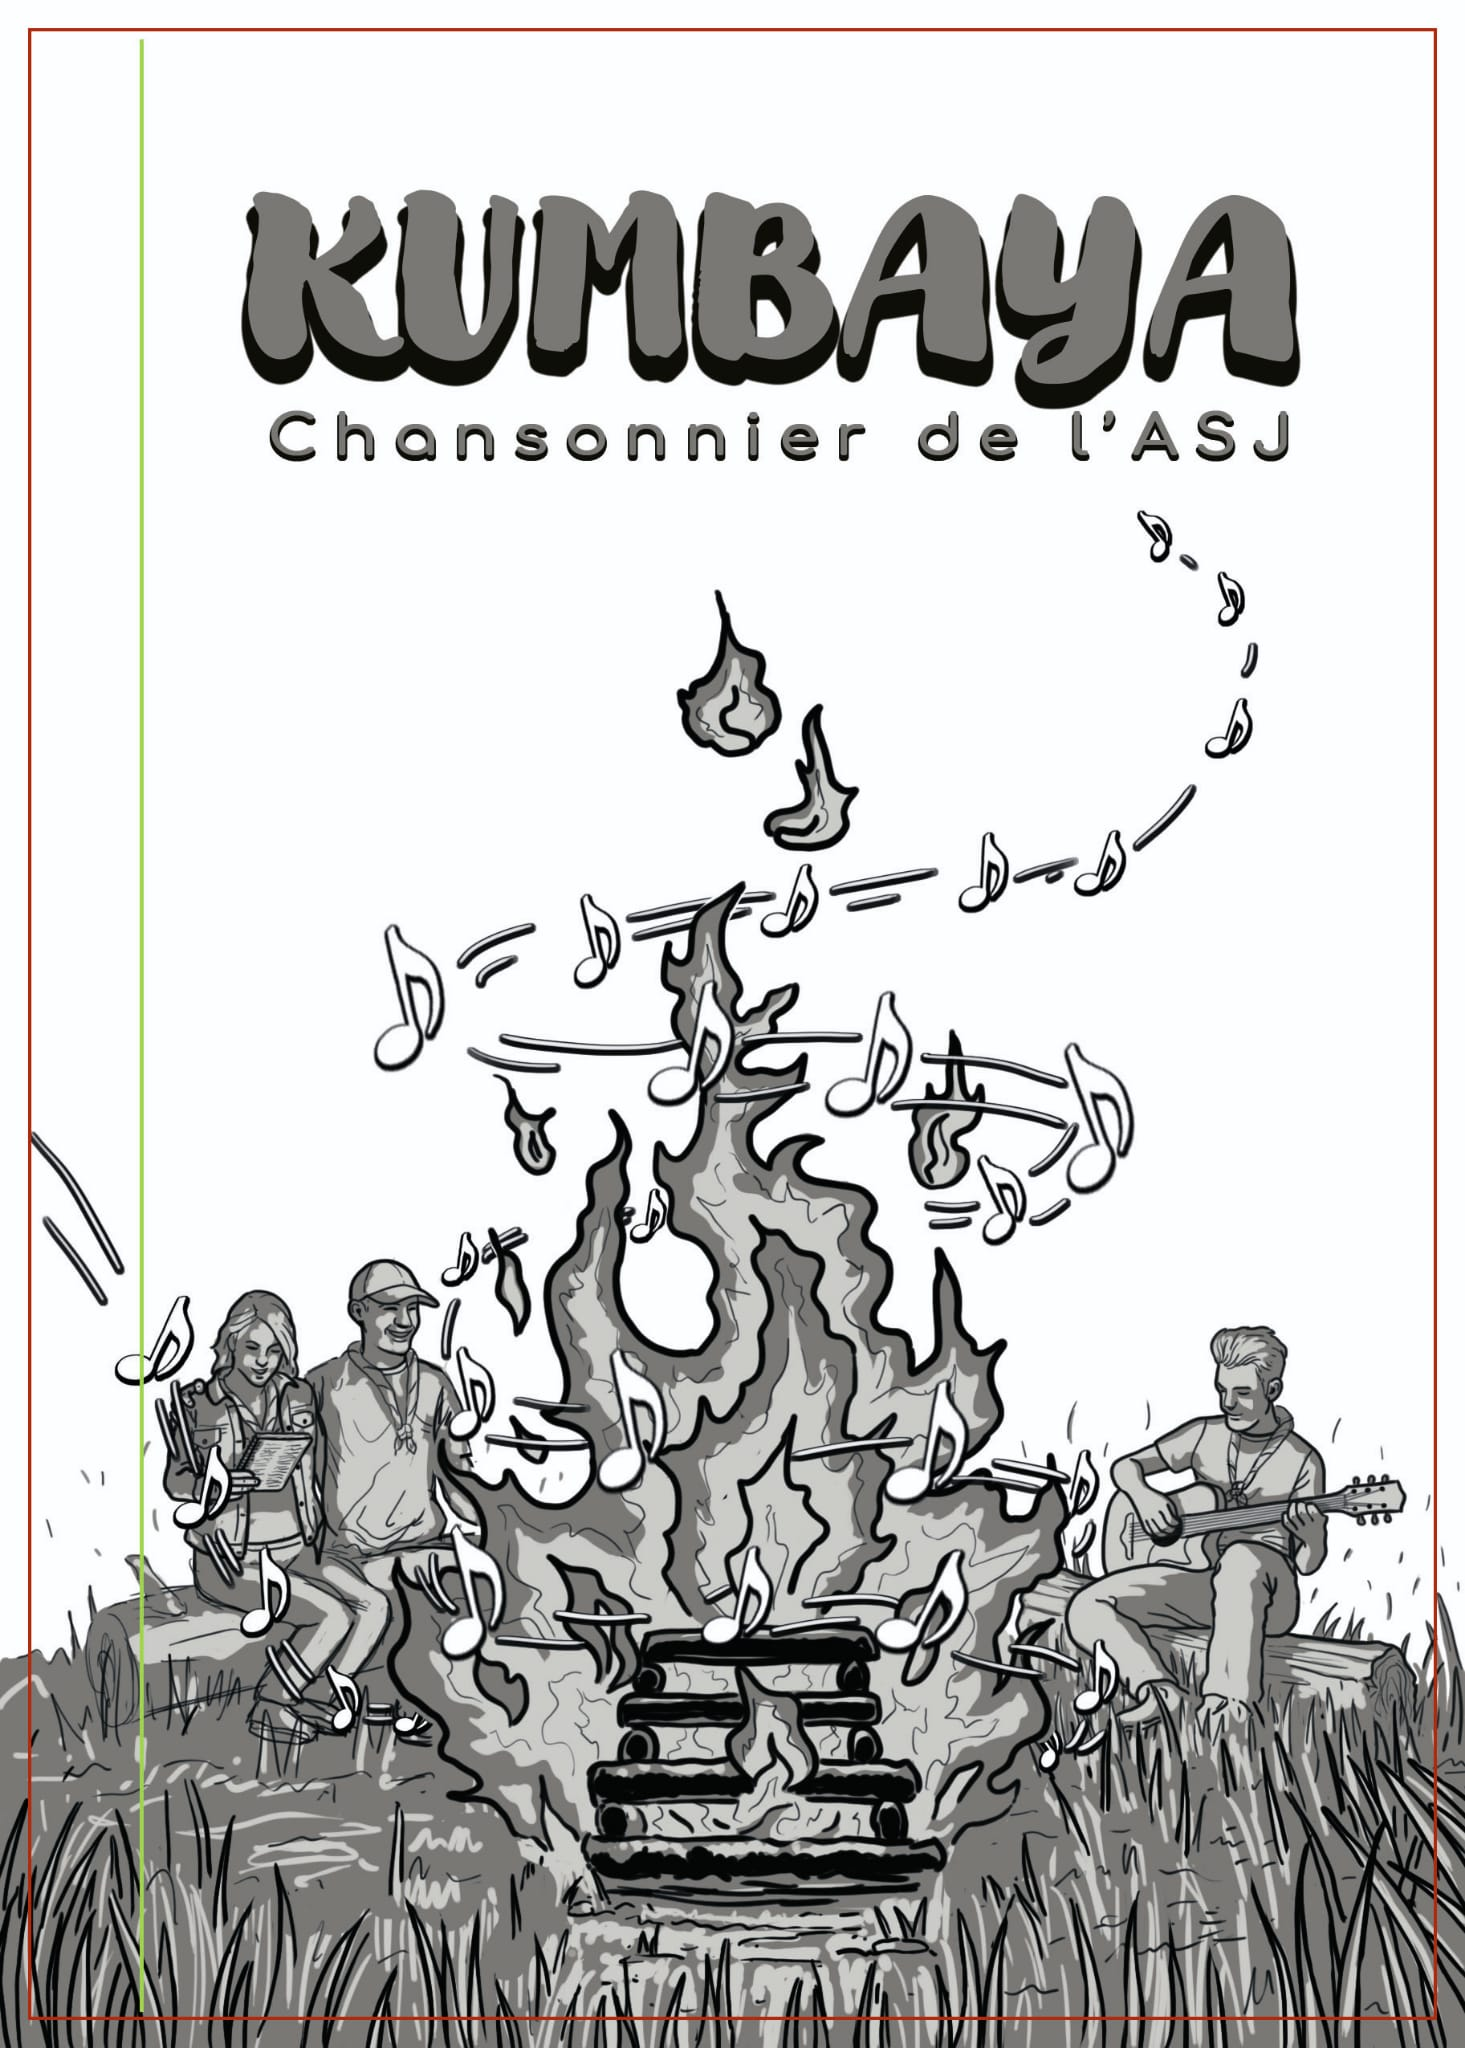
\includegraphics[width=154truemm,height=216truemm]{couverture.jpeg}}}%
}
\newpage
\
\newpage
\
\newpage
\clearpage
\restoregeometry

% \showindex[2]{Index alphabétique}{mainindex}
\section*{Avant-propos}
\small Tu tiens entre tes mains la toute nouvelle édition du Kumbaya : le chansonnier de l'Association du Scoutisme Jurassien ! Pensé pour toutes celles et ceux qui aiment pousser la chansonnette autour d'un feu de camp, guitare en bandoulière, ou encore micro à la main pour chanter en mode karaoké grâce à notre playlist Spotify “Kumbaya”. Ce recueil t'accompagnera dans tes moments musicaux et festifs.

Au cœur de sa conception, plusieurs objectifs ont guidé notre équipe. D'abord, nous avons souhaité rafraîchir le répertoire musical, en gardant nos classiques tout en faisant la part belle aux années 1990-2020 et à la découverte de nouvelles et nouveaux artistes. Plusieurs reprises contemporaines sont ainsi mentionnées aux côtés des artistes d'origine.

Ensuite, nous avons souhaité offrir un chansonnier accessible pour encourager la pratique musicale, en particulier à la guitare. Les accords figurent dans ce recueil accompagnés d'une méthodologie pratique pour que les grands rêveurs ainsi que les débutant·e·s osent enfin se lancer à la gratte !
Par ailleurs, notre chansonnier vise à intégrer davantage les branches Louveteaux et Route dans son répertoire. Des chansons pour les plus petit·e·s et autres bans figurent ainsi dans notre table des matières. D'autre part, plusieurs chansons adressées à un public plus majeur dont les paroles portent sur la consommation de substances addictives ainsi que des idées potentiellement violentes, politiques ou morales subjectives de leurs artistes sont marquées du signe *. Notre équipe souhaite laisser à chaque adulte la réflexion du choix des chansons et le soin d'une prévention ou d'une remise en contexte adaptée.

Née d'une idée lancée à l'automne 2022 au large de la mer Égée, cette édition du Kumbaya est le fruit d'un travail collectif, nourri par les propositions des douze groupes de l'ASJ, de longues discussions entre passionné·e·s de chant, et d'un élan enthousiaste printanier pour le faire aboutir à temps pour le camp JUBACA. Son contenu trouve ses origines dans le Kumbaya de l'ASJ (1997), la première édition du Petit Romand (1998), le Faramaz du Groupe Perceval (2013) et la nouvelle édition du P'tit Romand du scoutisme genevois (2023).

Alors que s'élève la première note de la farandole, que crépitent les braises ou que la sono s'allume… nous te souhaitons de belles veillées sous les étoiles!

L'équipe Kumbaya de l'Association du Scoutisme Jurassien (ASJ)

Juillet 2025

\newpage
\begin{multicols}{\nbcols}
	\begin{songs}{}
		\beginsong{1987}[by={Calogero (2017)}]

\beginverse
Tu t'sou\MultiwordChords\[Ré]viens
Les couleurs sur les bas\MultiwordChords\[Sim]kets
Les crayons dans les cas\MultiwordChords\[La]settes
Je rembobine
Tu t'sou\MultiwordChords\[Ré]viens
Tous ces rêves plein nos disq\MultiwordChords\[Sim]uettes
À Paris c'était les S\MultiwordChords\[La]tates
198\MultiwordChords\[Mim]7 \MultiwordChords\[La]
\endverse

\beginchorus
Il \MultiwordChords\[Ré]y a certains jours où \MultiwordChords\MultiwordChords\[La]je reprends mon skate
Et j\MultiwordChords\[Si7]e vais faire un tour en 19\MultiwordChords\[Fa#m]87 \MultiwordChords\[Sol] \MultiwordChords\[Mim] \MultiwordChords\[La]
Il \MultiwordChords\[Ré]y a certains jours dans \MultiwordChords\[La]lesquels je me jette
Et \MultiwordChords\MultiwordChords\[Sim7]je suis de retour en 19\MultiwordChords\[Fa#m]87 \MultiwordChords\[Sol] \MultiwordChords\[Mim] \MultiwordChords\[La]
Tu \MultiwordChords\[Ré]sais de tous ces jours y'a \MultiwordChords\[La]rien que je regrette
Mais \[Sim7]parfois je retourne en \MultiwordChords\[Fa#m]mille neuf cent quatre-vingt-\MultiwordChords\[Sol]sept, en 87
\endchorus

\beginverse
Tu t'souviens
Les survêts et les houppettes
Sabrina et 7 sur 7
Dans la cuisine c'était rien
Que 12 mois sur la planète
L'URSS, INXS
On chantait I want your sex
\endverse

\beginchorus
Refrain
\endchorus

\beginverse
Tu verras bien qu'un jour une chanson dans la tête
Tu l'auras à ton tour ton 1987
Tu verras bien qu'un jour une chanson dans la tête
Tu l'auras à ton tour ton 1987
C'est tout ce que je te souhaite
Tu l'auras à ton tour ton 1987
C'est tout ce que je te souhaite
Tu l'auras à ton tour ton 1987
C'est tout ce que je te souhaite
Tu l'auras à ton tour ton 1987
Tu t'souviens
\endverse
\endsong

\beginsong{99 Luftballons}[by={Nena (1983)}]

\beginverse
\MultiwordChords\[Ré]Hast du etwas \MultiwordChords\[Mim]Zeit für mich ?
Dann \MultiwordChords\[Sol]singe ich ein \MultiwordChords\[La]Lied für dich
Von \MultiwordChords\[Ré]99 \MultiwordChords\[Mim]Luftballons
Auf \MultiwordChords\[Sol]ihrem Weg zum \MultiwordChords\[La]Horizont
\MultiwordChords\[Ré]Denkst du vielleicht \MultiwordChords\[Mim]g'rade an mich
Dann \MultiwordChords\[Sol]singe ich ein \MultiwordChords\[La]Lied für dich
Von \MultiwordChords\[Ré]99 \MultiwordChords\[Mim]Luftballons
Und \MultiwordChords\[Sol]das sowas von \MultiwordChords\[La]sowas kommt
\endverse

\beginverse
99 Luftballons
Auf ihrem Weg zum Horizont
Hielt man für UFOs aus dem All
Darum schickte ein General
Eine Fliegerstaffel hinterher
Alarm zu geben, wenn es so wäre
Dabei waren da am Horizont
Nur 99 Luftballons
\endverse

\beginverse
99 Düsenflieger
Jeder war ein großer Krieger
Hielten sich für Captain Kirk
Das gab ein großes Feuerwerk
Die Nachbarn haben nichts gerafft
Und fühlten sich gleich angemacht
Dabei schoss man am Horizont
Auf 99 Luftballons
\endverse

\beginverse
99 Kriegsminister
Streichholz und Benzinkanister
Hielten sich für schlaue Leute
Witterten schon fette Beute
Riefen Krieg und wollten Macht
Mann, wer hätte das gedacht ?
Dass es einmal soweit kommt
Wegen 99 Luftballons
\endverse

\beginverse
99 Jahre Krieg
Ließen keinen Platz für Sieger
Kriegsminister gibt es nicht mehr
Und auch keine Düsenflieger
Heute ziehe ich meine Runden
Sehe die Welt in Trümmern liegen
Habe einen Luftballon gefunden
Denke an dich und lasse ihn fliegen
\endverse
\endsong

\beginsong{À nos souvenirs}[by={Trois cafés gourmands (2018)},sr={Capo IV}]

\beginverse
Comment puis-je oubl\MultiwordChords\[Lam]ier
Ce coin de para\MultiwordChords\[Fa]dis ?
Ce petit bout de \MultiwordChords\[Do]terre
Où vit encore mon \MultiwordChords\[Sol]père
\endverse

\beginverse
Comment pourrais-je \MultiwordChords\[Lam]faire
Pour me séparer \MultiwordChords\[Fa]d'elle ?
Oublier qu'on est \MultiwordChords\[Do]frères
Belle Corrèze char\MultiwordChords\[Sol]nelle
Oublier ce ma\MultiwordChords\[Lam]tin que tu es Par\MultiwordChords\[Fa]isien
Que t'as de l'eau dans le \MultiwordChords\[Do]vin
Que tu es parti \MultiwordChords\[Sol]loin
\endverse

\beginverse
Ce n'était pas ma faute
On joue des fausses notes
On se trompe de chemin
Et on a du chagrin
On se joue tout un drame
On a des vagues à l'âme
Tu as du mal au cœur
Tu as peur du bonheur
\endverse

\beginverse
Acheter des tableaux
Et des vaches en photo
C'est tout ce que t'as trouvé
Pour te la rappeler
Vous me trouvez un peu con
N'aimez pas ma chanson
\endverse

\beginverse
Vous me croyez bizarre
Un peu patriotard
Le fruit de ma réflexion
Ne touchera personne
Si vos pas ne résonnent
Jamais dans ma région
\endverse

\beginverse
C'est pire qu'une religion
Au-delà d'une confession
Je l'aime à en mourir
Pour le meilleur et pour le pire
Et si je monte au ciel
Il y aura peut-être Joël
\endverse

\beginverse
Guillaume et Jeremy
Et mon cousin Piedri
Yoan sera en voyage
Dans un autre pays
Allez fais tes bagages
Viens rejoindre tes amis
\endverse

\beginverse
On veut du Clody Musette
À en perdre la tête
On veut un dernier Chabrol
Un petit coup de gnôle
Les yeux de nos grands-mères
La voix de nos grands-pères
L'odeur de cette terre
Vue sur les Monédières
\endverse

\beginverse
C'est pire qu'un testament
Au-delà d'une confidence
On est des petits-enfants
De ce joli coin de France
Enterrez-nous vivants
Bâillonnés s'il le faut
Mais prenez soin avant
De remplir notre jabot
\endverse

\beginverse
La relève est pour toi
Notre petit Lucas
On t'laisse en héritage la piste
Nous, on dégage
Le temps nous a gâtés
On en a bien profité
On a des souvenirs en tête
Ce soir, faisons la fête
\endverse

\beginchorus
Acceptez ma rengaine
Elle veut juste dire je t'aime
Soyez sûr, j'en suis fier
J'ai la Corrèze en cathéter
D'être avec vous ce soir
J'ai le cœur qui pétille
Mimi, sers-nous à boire
On a les yeux qui brillent
\endchorus

\beginverse
\bis{Papayapapa, papayapapa, papayapapa
    Paya, papayapapa}{4}
\endverse

\beginchorus
Refrain
\endchorus
\endsong

\beginsong{L'agriculteur}[by={Ridan (2003)}]

\beginverse
J'allume mon p\MultiwordChords\[Lam]oste de tél\MultiwordChords\[Do]é
Pour admir\MultiwordChords\[Sol]er ce qu'il s'y p\MultiwordChords\[Lam]asse
Un milliard\MultiwordChords\[Fa]aire s'envoie en l\MultiwordChords\[Rém]'air
Toute l'at\MultiwordChords\[Mim]mosphère pour voir l'esp\MultiwordChords\[Lam]ace
J'troque son bol d\MultiwordChords\[Lam]'air et sa cuil\MultiwordChords\[Do]lère
Contre un p'tit v\MultiwordChords\[Sol]erre sur ma ter\MultiwordChords\[Lam]rasse
J'en ai ras-le-b\MultiwordChords\[Fa]ol de tout ce bét\MultiwordChords\[Rém]on
J'ai la fol\MultiwordChords\[Mim]ie des grands esp\MultiwordChords\[Lam]aces
\[Lam] \[Do] \[Sol] \[Lam] \brk J'en ai ras-le-b\MultiwordChords\[Fa]ol de tout ce bét\MultiwordChords\[Rém]on
J'ai la fol\MultiwordChords\[Mim]ie des grands esp\MultiwordChords\[Lam]aces
Mais qu'est-ce qui s\MultiwordChords\[Lam]e passe dans nos p'tites t\MultiwordChords\[Do]êtes ?
On s'entasse t\MultiwordChords\[Sol]ous comme des sard\MultiwordChords\[Lam]ines
Dans les grosses b\MultiwordChords\[Fa]oîtes que l'on cons\MultiwordChords\[Rém]erve
Le p'tit pois\MultiwordChords\[Mim]son doit suivre sa l\MultiwordChords\[Lam]igne
\[Lam] \[Do] \[Sol] \[Lam] \brk Dans les grosses b\MultiwordChords\[Fa]oîtes que l'on cons\MultiwordChords\[Rém]erve
Le p'tit pois\MultiwordChords\[Mim]son doit suivre sa l\MultiwordChords\[Lam]igne
\endverse

\beginchorus
Et puis m\MultiwordChords\[Lam]erde! J'ai décid\MultiwordChords\[Do]é de vivre l\MultiwordChords\[Sol]oin sur la col\MultiwordChords\[Lam]line
Vivre s\MultiwordChords\[Fa]eul dans une mais\MultiwordChords\[Rém]on avec la v\MultiwordChords\[Mim]ue sur ma rais\MultiwordChords\[Lam]on
J'préfère vivre p\MultiwordChords\[Lam]auvre avec mon â\MultiwordChords\[Do]me, que vivre r\MultiwordChords\[Sol]iche avec la l\MultiwordChords\[Lam]eur
Et si le b\MultiwordChords\[Fa]lé m'file du bonh\MultiwordChords\[Rém]eur, j'me ferais p\MultiwordChords\[Mim]'têt' agricult\MultiwordChords\[Lam]eur
\MultiwordChords\[Lam] \MultiwordChords\[Do] \MultiwordChords\[Sol] \MultiwordChords\[Lam] \brk Et si le b\MultiwordChords\[Fa]lé m'file du bonh\MultiwordChords\[Rém]eur, j'me ferais p\MultiwordChords\[Mim]'têt' agricult\MultiwordChords\[Lam]eur
\endchorus

\beginverse
Y a trop d'feux rouges dans les grandes villes
J'ai préféré me mettre au vert
J'ai plus d'bonheur à vivre en paix
Que d'm'admirer au fond d'un verre
J'boirai l'eau saine de mon ruisseau
Plutôt qu'l'eau sale du fond de la Seine
Chargée en plomb et en histoire
Que la surface ne laisse plus voir
Chargée en plomb et en histoire
Que la surface ne laisse plus voir
J'ferai des bornes pour m'éloigner
Pour m'retrouver face au miroir
Juste une seconde de vérité
Pour qu'mon passé coule sous les ponts
J'ferai des bornes pour m'éclipser
Pour m'retrouver face à que dalle
Juste une seconde de vérité
Pour contempler ce qu'on est tous
\endverse

\beginchorus
Refrain
\endchorus

\beginverse
Ça fait longtemps que j'n'ai plus vu
Ce coin d'soleil à l'horizon
Ça fait longtemps que j'l'attendais
La petite lueur de la raison
Une petite chanson au clair de lune
Pour réchauffer le cœur de pierre
Le grand retour à l'essentiel
Le feu de bois éclaire le ciel
Le grand retour à l'essentiel
Le feu de bois éclaire le ciel
La mélodie de la nature
Reprend ses droits sur la folie
C'est toute la vie qui nous observe
Que l'on oublie au fil du temps
La mélodie, celle de la vie
Que l'on consume à chaque instant
Tous nos acquis s'écrasent au sol
Et j'ai choisi la clé des champs
Tous nos acquis s'écrasent au sol
Et j'ai choisi la clef des champs
\endverse

\beginchorus
\bis{Refrain}{2}
\endchorus
\endsong

\beginsong{Ah les crocodiles !}[by={Jacques Offenbach (1856), Julien Doré (2024)}]

\beginverse
\MultiwordChords\[Ré]Un crocodile s'en allant à la \MultiwordChords\[La]guerre
\MultiwordChords\[Mi]Disait au revoir \MultiwordChords\[Mi7]à ses petits-\MultiwordChords\[La]enfants
\MultiwordChords\[Ré]Traînant ses pieds, ses pieds dans la pouss\MultiwordChords\[La]ière
\MultiwordChords\[Mi]Il s'en allait combattre les élé\MultiwordChords\[La7]phants
\endverse

\beginchorus
\bis{\MultiwordChords\[Ré]Ah' les crocrocros, les crocrocros, les croco\MultiwordChords\[La7]diles
    Sur les bords du Nil, ils sont partis, n'en parlons \MultiwordChords\[Ré]plus}{2}
\endchorus

\beginverse
Il fredonnait une marche militaire
Dont il mâchait les mots à grosses dents
Quand il ouvrait la gueule tout entière
On croyait voir ses ennemis dedans
\endverse

\beginverse
Il agitait sa grande queue à l'arrière
Comme s'il était d'avance triomphant
Les animaux devant sa mine altière
Dans les forêts s'enfuyaient tout tremblants
\endverse

\beginverse
Un éléphant parut et sur la terre
Se prépara ce combat de géants
Mais près de là courait une rivière
Le crocodile s'y jeta subitement
\endverse

\beginverse
Et tout rempli d'une crainte salutaire
Il s'en retourna vers ses petits-enfants
Notre éléphant, d'une trompe plus fière
Voulut alors accompagner ce chant
\endverse
\endsong

\beginsong{Aïcha}[by={Khaled (1996)},sr={Capo III}]

\beginverse
\MultiwordChords\[Mim] Comme \MultiwordChords\[Do]si je n'ex\MultiwordChords\[Sol]istais \MultiwordChords\[Ré]pas
\MultiwordChords\[Mim] Elle e\MultiwordChords\[Do]st passée à côt\MultiwordChords\[Sol]é de \MultiwordChords\[Ré]moi
\MultiwordChords\[Mim] Sans un \MultiwordChords\[Do]regard, \MultiwordChords\[Sol]reine de \MultiwordChords\[Ré]Saba
\MultiwordChords\[Mim] J'ai \MultiwordChords\[Do]dit “Aïcha, prends, tout \MultiwordChords\[Sol]est pour t\MultiwordChords\[Ré]oi”
\endverse

\beginverse
Voici les perles, les bijoux
Aussi l'or autour de ton cou
Les fruits bien mûrs au goût de miel
Ma vie, Aïcha, si tu m'aimes
J'irai où ton souffle nous mène
Dans les pays d'ivoire et d'ébène
J'effacerai tes larmes, tes peines
Rien n'est trop beau pour une si belle, oh!
\endverse

\beginchorus
\MultiwordChords\[Mim] Aïc\MultiwordChords\[Do]ha, Aïcha, \MultiwordChords\[Sol]écoute-m\MultiwordChords\[Ré]oi
\MultiwordChords\[Mim] Aïc\MultiwordChords\[Do]ha, Aïcha, \MultiwordChords\[Sol]t'en va p\MultiwordChords\[Ré]as
\MultiwordChords\[Mim] Aïc\MultiwordChords\[Do]ha, Aïcha, r\MultiwordChords\[Sol]egarde-m\MultiwordChords\[Ré]oi
\MultiwordChords\[Mim] Aïc\MultiwordChords\[Do]ha, Aïcha, r\MultiwordChords\[Sol]éponds-m\MultiwordChords\[Ré]oi
\endchorus

\beginverse
Je dirai les mots, les poèmes
Je jouerai les musiques du ciel
Je prendrai les rayons du soleil
Pour éclairer tes yeux de reine, oh!
\endverse

\beginchorus
Refrain
\endchorus

\beginverse
\MultiwordChords\[Misus4] \MultiwordChords\[Lam]Elle a dit, Garde tes t\MultiwordChords\[Fa]résors
\MultiwordChords\[Lam]Moi, je vaux mieux que tout ç\MultiwordChords\[Fa]a
\MultiwordChords\[Rém] Des barreaux sont des barreaux, même \MultiwordChords\[Sol]en or
Je veux les \MultiwordChords\[Misus4]mêmes dr\MultiwordChords\[Mi]oits que t\MultiwordChords\[Lam]oi
\MultiwordChords\[Fa] Et du respect pour chaque j\MultiwordChords\[Rém]our
\MultiwordChords\[Rém]Moi, je ne veux que de l'\MultiwordChords\[Misus4]amour \MultiwordChords\[Mi]
\endverse

\beginverse
\MultiwordChords\[Mim] Comme \MultiwordChords\[Do]si je n'ex\MultiwordChords\[Sol]istais \MultiwordChords\[Ré]pas
Elle est passée à côté de moi
Sans un regard, reine de Saba
J'ai dit Aïcha, prends, tout est pour toi
\endverse
\endsong

\beginsong{L'aigle noir}[by={Barbara (1970)}]

\beginverse
\MultiwordChords\[Ré]Un beau jour ou peut-être \MultiwordChords\[La]une nuit
\MultiwordChords\[Mim]Près d'un lac je m'étais endormie
Quand soudain semblant crever le ciel
Et venant de nulle part
Surgit un aigle noir
\endverse

\beginverse
Lentement les ailes déployées
Lentement je le vis tournoyer
Près de moi dans un bruissement d'ailes
Comme tombé du ciel
L'oiseau vint se poser
\endverse

\beginverse
Il avait les yeux couleur rubis
Et les plumes couleur de la nuit
A son front, brillant de mille feux
L'oiseau roi couronné
Portait un diamant bleu
\endverse

\beginverse
De son bec il a touché ma joue
Dans ma main il a glissé son cou
C'est alors que je l'ai reconnu
Surgissant du passé
Il m'était revenu
\endverse

\beginverse
Dis, l'oiseau, oh dis, emmène-moi
Retournons au pays d'autrefois
Comme avant dans mes rêves d'enfant
Pour cueillir en tremblant
Des étoiles, des étoiles
\endverse

\beginverse
Comme avant dans mes rêves d'enfant
Comme avant sur un nuage blanc
Comme avant, allumer le soleil
Etre faiseur de pluie
Et faire des merveilles
\endverse

\beginverse
L'aigle noir dans un bruissement d'ailes
Prit son vol pour regagner le ciel
\endverse

\beginverse
Un beau jour ou peut-être une nuit
Près d'un lac je m'étais endormie
Quand soudain semblant crever le ciel
Et venant de nulle part
Surgit un aigle noir
\endverse
\endsong

\beginsong{Allô le monde}[by={Pauline (2007)},sr={Capo I}]

\beginverse
Il pa\MultiwordChords\[Lam]raît que les nouv\MultiwordChords\[Fa]elles ne \MultiwordChords\[Do]sont pas si b\MultiwordChords\[Sol]onnes
Que le mora\MultiwordChords\[La]l des\MultiwordChords\[Fa]cend
Et que l\MultiwordChords\[Do]es forces t'aband\MultiwordChords\[Sol]onnent
J'en\MultiwordChords\[Lam]tends
Tous les \MultiwordChords\[Fa]gens
Par\MultiwordChords\[Do]ler de tes his\MultiwordChords\[Sol]toires
Que l'ave\MultiwordChords\[Lam]nir qui t'at\MultiwordChords\[Fa]tend
Se joue sur le \MultiwordChords\[Do]fil du ra\MultiwordChords\[Sol]soir
Qu'en est-\MultiwordChords\[Fa]il de l'a\MultiwordChords\[Sol]mour ?
Des \MultiwordChords\[Fa]larmes et de la \MultiwordChords\[Sol]peine ?
De la \MultiwordChords\[Fa]vie de tous les \MultiwordChords\[Sol]jours ?
Et d\MultiwordChords\[Fa]e la paix \MultiwordChords\[Sol]sereine ?
\endverse

\beginchorus
Allô le \MultiwordChords\[Lam]monde \MultiwordChords\[Fa]
\[Lam]Est-ce que tout va b\MultiwordChords\[Sol]ien ?
Allô le mon\MultiwordChords\[Lam]de \MultiwordChords\[Fa]
Je \MultiwordChords\[Lam]n'y comprends plus \MultiwordChords\[Sol]rien
Allô le mon\MultiwordChords\[Lam]de \MultiwordChords\[Fa]
\MultiwordChords\[Lam]Prends soin de \MultiwordChords\[Sol]toi
Allô le mon\MultiwordChords\[Lam]de \MultiwordChords\[Fa]
Ne te laisse \MultiwordChords\[Lam]pas aller \MultiwordChords\[Sol]
Comme \MultiwordChords\[Lam]ç\MultiwordChords\[Fa]a\MultiwordChords\[Lam] \MultiwordChords\[Sol]
\MultiwordChords\[Sol]Comme \MultiwordChords\[Lam]ç\MultiwordChords\[Fa]a\MultiwordChords\[Lam] \MultiwordChords\[Sol]
\endchorus

\beginverse
Quel est le nom du mal dont tu subis la fièvre
Les étranges idéaux, les hystéries funèbres ?
Dis-moi ce que je peux faire de ma petite place
Quels sont les actes et les mots qui peuvent t'aider à faire face ?
Pousser à la révolte
Pour faire le premier pas
Semer pour qu'on récolte
Pour crier mon effroi
\endverse

\beginverse
\[Lam]Allô le \[Rém]monde
\[Fa] Allô le \[Sol]monde
\[Lam]Allô le \[Rém]mond\[Fa]e \[Sol]
Allô le monde
Allô le monde
\endverse

\beginverse
Allô le monde
Est-ce que tout va bien ?
Allô le monde
Allô le monde
Prends soin de toi
Allô le monde
Le monde, le monde, le monde, le monde
Le monde, le monde, le monde, le monde
Allô le monde
Allô le monde, le monde
\endverse
\endsong

\beginsong{L'alphabet scout}[by={Traditionnel}]

\beginverse
Un j\MultiwordChords\[Do]our la troupe campa, A \MultiwordChords\[Sol]A A
La pluie se mit à tomber, \MultiwordChords\[Sol7]B B \MultiwordChords\[Do]B
L'orage a tout cassé, C C \MultiwordChords\[Sol]C
Faillit nous inon\MultiwordChords\[Do]der, A \MultiwordChords\[Sol]B C \MultiwordChords\[Do]D
\endverse

\beginverse
Le chef s'est écrié, E E E
A son adjoint Joseph, F F F
Fais-nous vite à manger, G G G
Les scouts sont sous la bâche E F G H
\endverse

\beginverse
Les pinsons dans leur nid, I l I
Les cerfs dans leur logis, J J J
Chahutent, quel fracas, K K K
Avec les hirondelles, I J K L
\endverse

\beginverse
Joseph nous fit d'la crème, M M M
Et du lapin d'Garenne, N N N
Et même du cacao, O O O
Mes amis quel souper, M N O P
\endverse

\beginverse
Soyez bien convaincus, QQ Q
Que la vie au grand air, R R R
Fortifie la jeunesse, S S S
Et lui rend la santé, Q R S T
\endverse

\beginverse
Maint'nant qu'il ne pleut plus, U U U
Les scouts peuvent se sauver, V V V
Le temps est au beau fixe, X X X
Plus besoin qu'on les aide, U V XZ
\endverse
\endsong

\beginsong{L'amour brille sous les étoiles}[by={Elton John, Tim Rice \- Le Roi Lion (1994)}]

\beginverse
\MultiwordChords\[Sol] C'est terrible c'est aff\MultiwordChords\[Ré]reux \- Quoi ?
Et \MultiwordChords\[Sol]ils se moquent de \MultiwordChords\[Ré]tout \- Qui ?
L'a\MultiwordChords\[Sol]mour s'amène et \MultiwordChords\[Sim]nous pauvres pouilleux
Ils \MultiwordChords\[Mim]nous jettent tous les \MultiwordChords\[La]deux \- Oh !
Sous \MultiwordChords\[Sol]les diamants des \MultiwordChords\[Ré]étoiles
Quel \MultiwordChords\[Sol]magique uni\MultiwordChords\[Ré]vers
Mais\MultiwordChords\[Sol] dans cette ro\MultiwordChords\[Sim]mantique atmosp\MultiwordChords\[Sol]hère
Ça \MultiwordChords\[Fa]sent mauvais dans \MultiwordChords\[Ré]l'air
\endverse

\beginverse
\MultiwordChords\[Sol] L'amour b\MultiwordChords\[Ré]rille sous \MultiwordChords\[Mim]les étoi\MultiwordChords\[Do]les
\MultiwordChords\[Sol] D'une étran\MultiwordChords\[Do]ge lumiè\MultiwordChords\[Ré]re
\MultiwordChords\[Do] La Terre en\MultiwordChords\[Sol]tière
En \MultiwordChords\[Mim]parfaite h\MultiwordChords\[Do]armonie
Vit \MultiwordChords\[Lam]un mo\MultiwordChords\[Fa]ment ro\MultiwordChords\[Ré]yal
\endverse

\beginverse
Je voudrais lui dire je t'aime
Mais comment lui avouer
Mon secret mes problèmes
Impossible
Elle serait trop blessée
\endverse

\beginverse
Quel lourd secret cache-t-il
Derrière tant de rancœur
Moi je sais qu'il est ce roi en exil
Qui règne dans mon coeur
\endverse

\beginverse
L'amour brille sous les étoiles
D'une étrange lumière
La Terre entière
En parfaite harmonie
Vit sa plus belle histoire
\endverse

\beginverse
L'amour brille sous les étoiles
Illuminant leurs coeurs
Sa lumière éclaire à l'infini
Un sublime espoir
\endverse

\beginverse
S'ils s'enfuient vers
Leur rêve ce soir
Dans leur folle ronde
Si notre ami nous dit au revoir
Nous serons seuls au monde
\endverse
\endsong

\beginsong{Amour censure*}[by={Hoshi (2020)}]

\beginverse
\MultiwordChords\[Do] Au pla\MultiwordChords\[Sol]card mes senti\MultiwordChords\[Ré]ments
Surtout ne rien d\MultiwordChords\[Mim]ire, et faire semb\MultiwordChords\[Do]lant
Être à \MultiwordChords\[Sol]part, un peu penc\MultiwordChords\[Ré]hant
Au bout du nav\MultiwordChords\[Mim]ire, je coule doucement
\endverse

\beginverse
\MultiwordChords\[Do] Maman désolée, j'vais pas te mentir
\MultiwordChords\[Sol] C'est dur d'effacer tout ce qui m'attire
\MultiwordChords\[Ré] Un peu dépassée par tous mes dé\MultiwordChords\[Mim]sirs
\MultiwordChords\[Do] Papa c'est vrai, j'ai poussé de travers
\MultiwordChords\[Sol] J'suis une fleur qui se bat entre deux pierres
\MultiwordChords\[Ré] J'ai un cœur niqué par les bonnes maniè\MultiwordChords\[Mim]res
\endverse

\beginchorus
\MultiwordChords\[Do] Est-ce qu'on va un jour en finir
\MultiwordChords\[Sol] Avec la haine et les injures
\MultiwordChords\[Ré] Est-ce que quelqu'un viendra leur dire
\MultiwordChords\[Mim] Qu'on s'aime et que c'est pas impur
\MultiwordChords\[Do] Pour pas que j'pense à en finir
\MultiwordChords\[Sol] Vos coups m'ont donné de l'allure
\MultiwordChords\[Ré] Pour le meilleur et pour le pire
\MultiwordChords\[Mim] J'prendrai sa main un jour c'est sûr
\endchorus

\beginverse
\MultiwordChords\[Sol] Il n'y a pas d'amour cen\MultiwordChords\[Ré]sure
\MultiwordChords\[Mim] Il n'y a que d'l'amour sin\MultiwordChords\[Do]cère
\MultiwordChords\[Sol] Il n'y a pas d'amour cen\MultiwordChords\[Ré]sure
\MultiwordChords\[Mim] Il n'y a que d'l'amour sin\MultiwordChords\[Do]cère
\endverse

\beginverse
Travestir qui je suis vraiment
Faire taire la rumeur
Les mots sont tranchants
Se mentir à s'arracher les dents
Ils cherchent un docteur
On souffre sans être souffrants
\endverse

\beginverse
Maman désolée, j'ai pris tes calmants
C'est pas que j'voulais partir, mais c'est violent
J'voulais juste dormir un peu plus longtemps
Papa t'inquiète j'ai appris à courir
Moi aussi j'veux une famille à nourrir
On s'en fout près de qui j'vais m'endormir
\endverse

\beginchorus
\bis{Refrain}{2}
\endchorus

\beginverse
Il n'y a pas d'amour censure
Il n'y a que d'l'amour sincère
Il n'y a pas d'amour censure
Il n'y a que d'l'amour sincère
\endverse
\endsong

\beginsong{Amsterdam*}[by={Jacques Brel (1964)}]

\beginverse
Dans le p\MultiwordChords\[Lam]ort d'Amsterdam, y a des m\MultiwordChords\[Mim]arins qui chantent
Les rê\MultiwordChords\[Fa]ves qui les hantent, au lar\MultiwordChords\[Mim7]ge d'Amsterdam
Dans le p\MultiwordChords\[Lam]ort d'Amsterdam, y a des ma\MultiwordChords\[Mim]rins qui dorment
Comme d\MultiwordChords\[Fa]es ori\MultiwordChords\[Mi7]flammes le long d\MultiwordChords\[Lam]es berges mornes
Dans le p\MultiwordChords\[Do]ort d'Amsterdam, y a des ma\MultiwordChords\[Sol7]rins qui meurent
Pleins de bi\MultiwordChords\[Lam]ère et de drames aux pre\MultiwordChords\[Mi7]mières lueurs
Mais dans le p\MultiwordChords\[Fa]ort d'Amsterdam, y a des ma\MultiwordChords\[Mim]rins qui naissent
Dans la c\MultiwordChords\[Fa]haleur ép\MultiwordChords\[Mi7]aisse des lang\MultiwordChords\[Lam]ueurs océanes
\endverse

\beginverse
Dans le port d'Amsterdam, y a des marins qui mangent
Sur des nappes trop blanches des poissons ruisselants
Ils vous montrent des dents à croquer la fortune
A décroisser la Lune, à bouffer des haubans
Et ça sent la morue jusque dans le cœur des frites
Que leurs grosses mains invitent à revenir en plus
Puis se lèvent en riant, dans un bruit de tempête
Referment leur braguette et sortent en rotant
\endverse

\beginverse
Dans le port d'Amsterdam, y a des marins qui dansent
En se frottant la panse sur la panse des femmes
Et ils tournent et ils dansent comme des soleils crachés
Dans le son déchiré d'un accordéon rance
Ils se tordent le cou pour mieux s'entendre rire
Jusqu'à ce que tout à coup l'accordéon expire
Alors, le geste grave, alors le regard fier
Ils ramènent leur Batave jusqu'en pleine lumière
\endverse

\beginverse
Dans le port d'Amsterdam, y a des marins qui boivent
Et qui boivent et reboivent, et qui reboivent encore
Ils boivent à la santé des putains d'Amsterdam
De Hambourg ou d'ailleurs, enfin ils boivent aux dames
Qui leur donnent leur joli corps, qui leur donnent leur vertu
Pour une pièce en or, et quand ils ont bien bu
Se plantent le nez au ciel, se mouchent dans les étoiles
Et ils pissent comme je pleure sur les femmes infidèles
Dans le p\MultiwordChords\[Lam]ort d'Amsterdam, dans le p\MultiwordChords\[Mi7]ort d'Amsterdam\MultiwordChords\[Fa-Mi7-Lam]
\endverse
\endsong

\beginsong{Andalouse}[by={Kendji Girac (2014)},sr={Capo I}]

\beginverse
\MultiwordChords\[Mim] Tu viens le s\MultiwordChords\[Sim]oir
\MultiwordChords\[Lam] Danser sur \MultiwordChords\[Sim]des airs de guit\MultiwordChords\[Mim]are
Et puis tu b\MultiwordChords\[Sim]ouges
\MultiwordChords\[Lam] Tes cheveux n\MultiwordChords\[Sim]oirs, tes lèvres r\MultiwordChords\[Mim]ouges
Tu te bal\MultiwordChords\[Sim]ances
\MultiwordChords\[Lam] Le reste n'\MultiwordChords\[Sim]a pas d'import\MultiwordChords\[Mim]ance
Comme un sol\MultiwordChords\[Sim]eil
\MultiwordChords\[Lam] Tu me brûles \MultiwordChords\[Sim]et me réveilles
\MultiwordChords\[Mim]Tu as \MultiwordChords\[Sim]dans les yeux, l\MultiwordChords\[Lam]e Sud et le f\MultiwordChords\[Sim]eu
\MultiwordChords\[Mim]Je t'ai d\MultiwordChords\[Sim]ans la peau
\MultiwordChords\[Lam]Baila, baila, \MultiwordChords\[Sim]oh
\endverse

\beginchorus
\MultiwordChords\[Mim]Toi, toi, \MultiwordChords\[Sim]ma belle Andal\MultiwordChords\[Lam]ouse
Aussi \MultiwordChords\[Sim]belle que jal\MultiwordChords\[Mim]ouse
Quand tu \MultiwordChords\[Sim]danses, le temps s'arr\MultiwordChords\[Lam]ête
Je perds le \MultiwordChords\[Sim]nord, je perds la t\MultiwordChords\[Mim]ête
Toi, \MultiwordChords\[Sim]ma belle Espag\MultiwordChords\[Lam]nole
Quand tu \MultiwordChords\[Sim]bouges tes é\MultiwordChords\[Mim]paules
Je n'vois \MultiwordChords\[Sim]plus le monde aut\MultiwordChords\[Lam]our
C'est peut-\MultiwordChords\[Sim]être ça, l'amour
\endchorus

\beginverse
Des airs d'Orient
Le sourire et le cœur brûlant
Regard ébène
J'aime te voir bouger comme une reine
Ton corps ondule
Déjà mes pensées se bousculent
Comme la lumière
Il n'y a que toi qui m'éclaire
Tu as dans la voix
Le chaud et le froid
Je t'ai dans la peau
Baila, baila, oh
\endverse

\beginchorus
Refrain
\endchorus

\beginverse
Oh-yé-yé-yé, oh-oh, oh-oh
Oh-yé-yé-yé, oh-oh
Oh-yé-yé-yé, oh-oh, oh-oh
Oh-yé-yé-yé, oh-oh
\endverse

\beginchorus
\bis{Refrain}{2}
\endchorus
\endsong

\beginsong{L'arc-en-ciel}[by={Pellisier-Moulin}]

\beginchorus
\MultiwordChords\[Do]Viens mélanger tes cou\MultiwordChords\[Sol]leurs avec \MultiwordChords\[lam]moi
Réveiller le bon\MultiwordChords\[Fa]heur qui \MultiwordChords\[Sol]dort au fond de \MultiwordChords\[Do]toi
Faire jaillir la lu\MultiwordChords\[Sol]mière de nos \MultiwordChords\[Lam]vies
Improviser la \MultiwordChords\[Fa]fête au \MultiwordChords\[Sol]plein cœur de la \MultiwordChords\[Do]nuit
\endchorus

\beginverse
\MultiwordChords\[Fa]Tu connais la mi\MultiwordChords\[Sol]sère \MultiwordChords\[Do]qui condamne au si\MultiwordChords\[Lam]lence :
\MultiwordChords\[Fa]Prends la main de tes \MultiwordChords\[Sol]frères, i\MultiwordChords\[Do]nvente un pas \MultiwordChords\[Fa]dans\MultiwordChords\[Sol]e !
\endverse

\beginverse
Tu refoules tes larmes dans ta gorge nouée :
Oublie le bruit des armes, réapprends à chanter !
\endverse

\beginverse
Tu t'opposeras à la force qui tue la liberté :
Entrouvre ton écorce au soleil de l'été !
\endverse

\beginverse
Tu rêves d'innocence au lieu d'hypocrisie :
Retrouve ton enfance, recommence ta vie !
\endverse

\beginverse
Tu pardonnes sa haine au frère qui t'a blessé :
Laisse tomber ta gêne, donne-lui un baiser !
\endverse
\endsong

\beginsong{Aux arbres citoyens}[by={Yannick Noah (2006)},sr={Capo I}]

\beginverse
Le \MultiwordChords\[Mim]ciment dans les plaines coule jusqu'aux montagnes
Poi\MultiwordChords\[Ré]son dans les fontaines, dans nos \MultiwordChords\[Do]campagnes
De c\MultiwordChords\[Mim]yclones en rafales, notre histoire prend l'eau
Res\MultiwordChords\[Ré]te notre idéal, fa\MultiwordChords\[Do]ire les beaux
\endverse

\beginverse
S'acheter de l'air en barre, remplir la balance
Quelques pétrodollars, contre l'existence
De l'Équateur aux pôles, ce poids sur nos épaules
De squatteurs éphémères, maintenant, c'est plus drôle
\endverse
\beginchorus
\MultiwordChords\[Mim]Puisqu'il faut changer les choses
A\MultiwordChords\[Ré]ux arbres cito\MultiwordChords\[Do]yens
\MultiwordChords\[Mim]Il est grand temps qu'on propose
\MultiwordChords\[Ré]Un monde \MultiwordChords\[Do]pour demain
\endchorus

\beginverse
Aux arbres citoyens, quelques baffes à prendre
La veille est pour demain, des baffes à rendre
Faire tenir debout une armée de roseaux
Plus personne à genoux, fais passer le mot
\endverse

\beginverse
C'est vrai la Terre est ronde, mais qui viendra nous dire
Qu'elle l'est pour tout le monde et les autres à venir
\endverse

\beginverse
\bis{Refrain}{2}
\endverse
\beginverse
\MultiwordChords\[Ré] Plus le temps de savoir à qui \MultiwordChords\[Mim]la faute
\MultiwordChords\[Ré] De compter sur la chance ou \MultiwordChords\[Do]les autres
\MultiwordChords\[Lam7] Maintenant, on se \MultiwordChords\[Mim]bat
A\MultiwordChords\[Do]vec toi, moi, j'y croi\MultiwordChords\[Mim]s
\endverse

\beginchorus
Refrain
\endchorus
\endsong

\beginsong{L'aventurier}[by={Indochine (1982)}]

\beginverse
\MultiwordChords\[Mim]Égaré dans la \MultiwordChords\[Do]vallée infernale
Le \MultiwordChords\[Sol]héros s'appelle \MultiwordChords\[Lam]Bob Morane
\MultiwordChords\[Mim]À la recherche de l'\MultiwordChords\[Do]Ombre Jaune
Le \MultiwordChords\[Sol]bandit s'appelle Mister \MultiwordChords\[Lam]Kali Jones
\MultiwordChords\[Mim]Avec l'ami Bill \MultiwordChords\[Do]Ballantine
\MultiwordChords\[Sol]Sauvé de justesse des \MultiwordChords\[Lam]crocodiles
\MultiwordChords\[Mim]Stop au trafic des \MultiwordChords\[Do]Caraïbes
\MultiwordChords\[Sol]Escale dans l'opération \MultiwordChords\[Lam]Nadawieb
\endverse

\beginverse
\bis{\MultiwordChords\[Mim]La lalalaaa la l\MultiwordChords\[Do]alalaa, \MultiwordChords\[Sol]La lalala la \MultiwordChords\[Lam]lala-lalaa}{2}
\endverse

\beginverse
Le cœur tendre dans le lit de Miss Clark
Prisonnière du Sultan de Jarawak
En pleine terreur à Manicouagan
Isolé dans la jungle birmane
Emprisonnant les flibustiers
L'ennemi est démasqué
On a volé le collier de Civa
Le Maharadjah en répondra
\endverse

\beginverse
\bis{La lalalaaa la lalalaa, La lalala la lala-lalaa}{2}
\endverse
\beginchorus
\MultiwordChords\[Lam]Et soudain surgit \MultiwordChords\[Mim]face au vent
Le \MultiwordChords\[Sol]vrai héros de \MultiwordChords\[Ré]tous les temps
\MultiwordChords\[Lam]Bob Morane contre \MultiwordChords\[Mim]tout chacal
L'a\MultiwordChords\[Sol]venturier contre \MultiwordChords\[Ré]tout guerrier
\MultiwordChords\[Lam]Bob Morane contre \MultiwordChords\[Mim]tout chacal
L'a\MultiwordChords\[Sol]venturier contre \MultiwordChords\[Ré]tout guerrier
\endchorus

\beginverse
Dérivant à bord du Sampang
L'aventure au parfum d'Ylalang
Son surnom, Samouraï du Soleil
En démantelant le gang de l'Archipel
L'otage des guerriers du Doc Xhatan
Il s'en sortira toujours à temps
Tel l'aventurier solitaire
Bob Morane est le roi de la Terre
\endverse

\beginverse
\bis{La lalalaaa la lalalaa, La lalala la lala-lalaa}{2}
\endverse

\beginchorus
Refrain
\endchorus
\endsong

\beginsong{Balade jurassienne*}[by={Christophe Meyer (2003)}]

\beginverse
\MultiwordChords\[Do] Il pleut \MultiwordChords\[Fa]toujours à Pleu\MultiwordChords\[Do]jouse
Quand le temps s\MultiwordChords\[Sol]'éclaire à Réc\MultiwordChords\[Do]lère
J'ai cou\MultiwordChords\[Fa]ru à Courro\MultiwordChords\[Do]ux
M'émerveil\MultiwordChords\[Sol]ler à Merv\MultiwordChords\[Do]elier
\MultiwordChords\[Fa] Si j'ai failli manquer F\MultiwordChords\[Do]ahy
\MultiwordChords\[Fa] Je ne vais pas rater Les Ge\MultiwordChords\[Do]nevez
\MultiwordChords\[Lam] J'fais aussi un saut à Saul\MultiwordChords\[Sol]cy
Pour cette balade jura\MultiwordChords\[Do]ssienne
\endverse

\beginverse
\MultiwordChords\[Rém]La \MultiwordChords\[Sol]la \MultiwordChords\[Do]la la la \MultiwordChords\[Fa]la
\MultiwordChords\[Rém]la la la \MultiwordChords\[Sol]la la la \MultiwordChords\[Do]la
\endverse

\beginverse
J'ai visité mes amies d'Alle
Vic à Vicques puis celle de Lucelle
Assez près d'elle à Séprais
Elle m'a dit vers ma ferme à Vermes
Qu'elle était soûle à Soulce
Elle voulait que je la plaigne à Pleigne
Les cheveux dans l'vent à Damvant
C'est une balade jurassienne
\endverse

\beginverse
Chatouilleux à Châtillon
J'ai lu le Coran à Corban
Perdu mon savon à Courchavon
C'était dans une rose maison – j'ai vu
Le bon et la folle de Bonfol
Les soldats s'aligner à Lugnez
Se faire couper les courtes mèches
Dans cette balade jurassienne
\endverse

\beginverse
Quand vous montiez à Montignez
J'ai embrassé la joue du r'gard
À Charmoille sur un char de paille
Mis ma ceinture à St-Ursanne
Je recours à Rocourt
Car c'est aux Bois qu'on boit
Le taux d'alcool à Montenol
Dans cette balade jurassienne
\endverse

\beginverse
J'avais l'air affreux à Damphreux
Au court de la beuverie d'Ocourt
Même pas eu l'temps d'cuver à Coeuve
Pour s'bourrer l'gnon à Bourrignon
Quand les copains burent à Bure
Beurré au Raisin d'Beurnevésin
C'était soit hier à Soyhières ou peut-être avant-hier
dans cette balade jurassienne, je sais plus
\endverse

\beginverse
Un peu maraud à Muriaux
J'ai volé des pommes aux Pommerats
Mangé mon melon à Montmelon
Qu'avait un goût moite à Goumois
J'ai soupé à Soubey
Sans faire de bruit à Buix
J'm'endors sur la roche de Roche-d'Or
Pour cette balade jurassienne
\endverse
\endsong

\beginsong{La ballade des gens heureux}[by={Gérard Lenorman (1975)},sr={Capo V}]

\beginverse
Notre \MultiwordChords\[Do]vieille Terre est une étoile
Où toi aussi tu \MultiwordChords\[Rém]brilles un \MultiwordChords\[Sol]peu
\bis{Je viens te \MultiwordChords\[Rém]chanter \MultiwordChords\[Sol7]la bal\MultiwordChords\[Do]lade
    La ball\MultiwordChords\[Rém]ade des \MultiwordChords\[Sol7]gens heu\MultiwordChords\[Do]reux}{2}
\endverse

\beginverse
Tu n'as pas de titre ni de grade
Mais tu dis tu quand tu parles à Dieu
\bis{Je viens te chanter la ballade
    La ballade des gens heureux}{2}
\endverse

\beginverse
Journaliste pour ta première page
Tu peux écrire tout ce que tu veux
\bis{Je t'offre un titre formidable
    La ballade des gens heureux}{2}
\endverse

\beginverse
Toi qui a planté cet arbre
Dans ton petit jardin de banlieue
\bis{Je viens te chanter la ballade
    La ballade des gens heureux}{2}
\endverse

\beginverse
Il s'endort et tu le regardes
Comme un enfant, il te ressemble un peu
\bis{On vient lui chanter la ballade
    La ballade des gens heureux}{2}
\endverse

\beginverse
Toi la star du haut de ta vague
Descends vers nous tu nous verras mieux
\bis{On vient te chanter la ballade
    La ballade des gens heureux}{2}
\endverse

\beginverse
Roi de la drague et de la rigolade
Rouleur, flambeur ou gentil petit vieux
\bis{On vient te chanter la ballade
    La ballade des gens heureux}{2}
\endverse

\beginverse
Comme un choeur dans une cathédrale
Comme un oiseau qui fait ce qu'il veut
\bis{On vient te chanter la ballade
    La ballade des gens heureux}{2}
\endverse
\endsong

\beginsong{La ballade nord-irlandaise*}[by={Renaud (1991)}]

\beginverse
J'ai voulu plant\MultiwordChords\[Sol]er un \MultiwordChords\[Do]orang\MultiwordChords\[Sol]er
Là où la chan\MultiwordChords\[Mim]son n'en \MultiwordChords\[Lam]verra ja\MultiwordChords\[Ré]mais
Là où les \MultiwordChords\[Sol] arbres n'ont jamais don\MultiwordChords\[Mim]né
Que \MultiwordChords\[Do]des gre\MultiwordChords\[Sol]nades \MultiwordChords\[Do]dégoupil\MultiwordChords\[Sol]lées
\endverse

\beginverse
Jusqu'à Derry ma bien aimée
Sur mon bateau j'ai navigué
J'ai dit aux hommes qui se battaient
Je viens planter un oranger
\endverse

\beginverse
Buvons un verre, allons pêcher
Pas une guerre ne pourra durer
Lorsque la bière et l'amitié
Et la musique nous feront chanter
\endverse

\beginverse
Tuez vos dieux à tout jamais
Sous aucune croix l'amour ne se plaît
Ce sont les hommes, pas les curés
Qui font pousser les orangers
\endverse

\beginverse
Je voulais planter un oranger
Là où la chanson n'en verra jamais
Il a fleuri et il a donné
Les fruits sucrés de la liberté
\endverse
\endsong

\beginsong{La batelière}[by={Traditionnel}]

\beginverse
\MultiwordChords\[Do] Gentille batelière, \MultiwordChords\[Sol]laisse-là \MultiwordChords\[Sol7]ton ba\MultiwordChords\[Do]teau
Préfère à ta chaumière \MultiwordChords\[Sol]les honneurs \MultiwordChords\[Sol7]du châ\MultiwordChords\[Do]teau
\MultiwordChords\[Sol]J'irai cueil\MultiwordChords\[Sol7]lir \MultiwordChords\[Do]la fleur nouvelle
\MultiwordChords\[Ré]Chaque matin pour \MultiwordChords\[Sol]toi
Tu choisi\MultiwordChords\[Sol7]ras \MultiwordChords\[Do]rubis, dentelles
\MultiwordChords\[Ré]Blanche viens avec \MultiwordChords\[Sol]moi !
\endverse

\beginchorus
\MultiwordChords\[Sol] Non, non, non, non J'a\MultiwordChords\[Do]ime mieux mon p'tit bateau
Ma \MultiwordChords\[Sol]rame fle\MultiwordChords\[Sol7]xible sur l'\MultiwordChords\[Do]onde paisible
Et ma chaumière au bord de l'eau
Tra \MultiwordChords\[Sol]la la la \MultiwordChords\[Sol7]la la la \MultiwordChords\[Do]la la la la
La \MultiwordChords\[Sol]la la la \MultiwordChords\[Sol7]la, la \MultiwordChords\[Do]la la la la, la \MultiwordChords\[Fa]la la la \MultiwordChords\[Sol]la la \MultiwordChords\[Do]la la la la
La \MultiwordChords\[Sol]la la la \MultiwordChords\[Sol7]la, la \MultiwordChords\[Do]la la la la, la \MultiwordChords\[Fa]la la la \MultiwordChords\[Sol]la la \MultiwordChords\[Do]la
\endchorus

\beginverse
Belle enfant qu'au rivage on entend chaque soir
Malgré les vents, l'orage, dire des chants d'espoir !
Tu reverras dans la vallée
Tes chalets et tes bois
Tu ne seras plus isolée
Blanche viens avec moi !
\endverse

\beginverse
Rien ne trouble ton âme, rien ne trouble ton cœur
Tu doutes de ma flamme, tu ris de ma douleur
Que te faut-il enfant cruelle Pour vaincre ton dédain
Te faire oublier ta nacelle ?
Veux-tu mon cœur, ma main ?
\endverse

\beginverse
Ah ! Ah ! Cette fois, mon seigneur
Tra la la la
Je veux bien vous donner mon cœur
Tra la la la
\endverse
\endsong

\beginsong{Le beau tambour}[by={Henri Dès (1986)}]

\beginverse
\bis{J'ai re\MultiwordChords\[Mi]çu, plan, plan
    J'ai reçu, plan, plan
    J'ai reçu un b\MultiwordChords\[Si7]eau tamb\MultiwordChords\[Mi]our
    Et je joue, plan, plan
    Et je joue, plan, plan
    Et je joue quand \MultiwordChords\[Si7]il fait j\MultiwordChords\[Mi]our
    Et quand \MultiwordChords\[La]il fait n\MultiwordChords\[Mi]uit, et le m\MultiwordChords\[La]ercre\MultiwordChords\[Mi]di
    Et quand p\MultiwordChords\[La]apa d\MultiwordChords\[Mi]ort enc\MultiwordChords\[Si7]ore
    Et pour l\MultiwordChords\[Mi]es vois\MultiwordChords\[Si7]ins, le dima\MultiwordChords\[Mi]nche mat\MultiwordChords\[Si7]in
    Je vais d\MultiwordChords\[Mi]ans le co\MultiwordChords\[Si7]rrid\MultiwordChords\[Mi]or
}{6}
\endverse
\endsong

\beginsong{Bella ciao*}[by={Auteur anonyme (1944)},sr={Capo V}]

\beginverse
Una mat\MultiwordChords\[Lam]tina mi son sveg\MultiwordChords\[Lam]liato
O bella \MultiwordChords\[Lam]ciao, bella ciao, bella \MultiwordChords\[Mi7]ciao ciao ciao
Una mat\MultiwordChords\[Rém]tina mi son sveg\MultiwordChords\[Lam]liato
Eo ho tro\MultiwordChords\[Mi7]vato l'inva\MultiwordChords\[Lam]sor
\endverse

\beginverse
O partigiano portami via
O bella ciao, bella ciao, bella ciao ciao ciao
O partigiano portami via
Che mi sento di morir
\endverse

\beginverse
E se io muoio da partigiano
O bella ciao, bella ciao, bella ciao ciao ciao
E se io muoio da partigiano
Tu mi devi seppellir
\endverse

\beginverse
Mi seppellire lassù in montagna
O bella ciao, bella ciao, bella ciao ciao ciao
Mi seppellire lassù in montagna
Sotto l'ombra di un bel fiore
\endverse

\beginverse
E le gente che passeranno
O bella ciao, bella ciao, bella ciao ciao ciao
E le genti che passeranno
Mi diranno: Che bel fior
\endverse

\beginverse
È questo il fiore del partigiano
O bella ciao, bella ciao, bella ciao ciao ciao
È questo il fiore del partigiano
Morto per la libertà
\endverse
\endsong

\beginsong{Berceuse tchèque}[by={Traditionnel}]

\beginverse
\MultiwordChords\[Do]Ecoute la prière
Qui du camp monte vers T\MultiwordChords\[Sol7]oi
\bis{Vers la grande lumiè\MultiwordChords\[Do]re
    \MultiwordChords\[Rém]Vers la pa\MultiwordChords\[Sol7]ix et vers la j\MultiwordChords\[Do]oie
}{2}
\endverse

\beginverse
Illumine la route
Où le monde nous attend
\bis{Que suivant la loi scoute
    Nous aidions les pauvres gens}{2}
\endverse

\beginverse
Donne à notre patrie
Divisée en ses frontières
\bis{La paix qui fut promise
    A ceux qui s'aiment en frères}{2}
\endverse
\endsong

\beginsong{Les bêtises}[by={Henri Dès (1991)}]

\beginchorus
\MultiwordChords\[Mi] Zoum zoum zoum-zoum-zoum
Zoum zouzoum \MultiwordChords\[Si7]zoum-\MultiwordChords\[Mi]zoum
\MultiwordChords\[Mi] C'est à l'école, tagadaga\MultiwordChords\[Si7]da
\MultiwordChords\[Mi] Qu'on apprend les bêti\MultiwordChords\[Si7]ses
\MultiwordChords\[Mi] C'est à l'école, tagadaga\MultiwordChords\[Si7]da
\MultiwordChords\[Mi] Qu'on apprend les bêti\MultiwordChords\[Si7]ses
\endchorus

\beginverse
Le grand Dédé — poil poil au nez
Devant toute la c\MultiwordChords\[Mi]lasse
\MultiwordChords\[Si7]Monte au tableau — poil poil au dos
Pour faire des gri\MultiwordChords\[Mi]maces
\endverse

\beginchorus
Refrain
\endchorus

\beginverse
Quand le Julien — poil poil aux mains
Raconte ses histoires
Elles sont si bêtes — poil aux chaussettes
Qu'on pleure dans nos mouchoirs
\endverse

\beginchorus
Refrain
\endchorus

\beginverse
Et la maîtresse — poil poil aux tresses
Qui pousse des soupirs
Quand Marion — poil au menton
Attrape le fou rire
\endverse

\beginchorus
Refrain
\endchorus

\beginverse
Et puis y'a moi — poil poil au doigt
Qui marche à quatre pattes
Pour chatouiller — poil au mollet
Ma voisine de droite
\endverse

\beginchorus
Refrain
\endchorus

\beginverse
Y'a la Thérèse — poil à la chaise
C'est la plus rigolote
Quand elle s'asseye — poil aux orteils
On lui voit sa culotte
\endverse

\beginchorus
Refrain
\endchorus

\beginverse
Heureusement — poil poil aux dents
Quand vient la sonnerie
Tout le monde s'arrête — poil aux baskets
Par ici la sortie
\endverse

\beginchorus
Refrain
\endchorus

\beginverse
Zoum zoum zoum-zoum-zoum
Zoum zouzoum zoum-zoum
\endverse
\endsong

\beginsong{Le bleu lumière}[by={Cerise Calixte \- Vaïana (2016)},sr={Capo IV}]

\beginverse
Le b\MultiwordChords\[Do]leu du ciel n'est pas le bleu de la m\MultiwordChords\[Rém]er
Ce bleu que moi je pr\MultiwordChords\[Lam]éfère
Sans vraiment savoir po\MultiwordChords\[Fa]urquoi
\MultiwordChords\[Do]J'aimerais tant rester fidèle à m\MultiwordChords\[Rém]a terre
Oublier le vent éph\MultiwordChords\[Lam]émère
J'ai essayé tant de f\MultiwordChords\[Fa]ois
J'ai beau d\MultiwordChords\[Lam]ire je reste, je ne partirai pas
Chacun d\MultiwordChords\[Sol]e mes gestes, chacun de mes pas
Me ram\MultiwordChords\[Do]ènent sans cesse
Malgré les promesses
Vers c\MultiwordChords\[Fam]e bleu lumière
L'hori\MultiwordChords\[Do]zon où la mer touche le ciel
Et \MultiwordChords\[Sol]m'appelle
Cache un trés\MultiwordChords\[Lam]or
Que tous ig\MultiwordChords\[Fa]norent
C'est le v\MultiwordChords\[Do]ent, doucement qui se lève
Et me r\MultiwordChords\[Sol]évèle
Le bleu de l'\MultiwordChords\[Lam]eau
Si je p\MultiwordChords\[Fam]ars j'irai plus loin et toujours plus haut
\endverse

\beginverse
Il faut aimer mon île et son histoire
Pour ceux qui veulent encore y croire
Oublier le temps qui passe
Il faut aimer mon île et son histoire
Et garder encore l'espoir
Un jour je trouverai ma place
Je peux les guider
Les rendre plus grands
Les accompagner
Je prendrai le temps
Mais cette voie cachée
Pense tout autrement
Je ne comprends pas
Le soleil vient danser sur la mer éternelle
Mais tous ignorent
Ces reflets d'or
Elle m'attend sous un tapis de lumière
La mer m'appelle
Moi je veux voir
Derrière les nuages de nouveaux rivages
L'horizon où la mer touche le ciel
Et m'appelle
Cache un trésor
Que tous ignorent
C'est le vent doucement qui se lève
Et me révèle
J'ai le droit
D'aller là-bas
\endverse
\endsong

\beginsong{Blowin' in the wind}[by={Bob Dylan (1962)}]

\beginverse
\MultiwordChords\[Ré]How many \MultiwordChords\[Sol]roads must a \MultiwordChords\[La]man walk \MultiwordChords\[Ré]down
Before you \MultiwordChords\[Sol]call him a \MultiwordChords\[Ré]man ?
\MultiwordChords\[Ré]How many \MultiwordChords\[Sol]seas must a \MultiwordChords\[La]white dove \MultiwordChords\[Ré]sail
Before she \MultiwordChords\[Sol]sleeps in the \MultiwordChords\[La]sand ?
Yes, and \MultiwordChords\[Ré]how many \MultiwordChords\[Sol]times must the \MultiwordChords\[La]cannonballs \MultiwordChords\[Ré]fly
Before they're \MultiwordChords\[Sol]forever \MultiwordChords\[Ré]banned ?
\endverse

\beginchorus
\MultiwordChords\[Sol]The answer, \MultiwordChords\[La]my friend, \MultiwordChords\[Ré]is blowin' in the \MultiwordChords\[Sol]wind
The answer is \MultiwordChords\[La]blowin' in the \MultiwordChords\[Ré]wind
\endchorus

\beginverse
Yes, and how many years must a mountain exist
Before it is washed to the sea ?
Yes, and how many years can some people exist
Before they're allowed to be free ?
Yes, and how many times can a man turn his head
And pretend that he just doesn't see ?
\endverse

\beginchorus
Refrain
\endchorus

\beginverse
Yes, and how many times must a man look up
Before he can see the sky ?
Yes, and how many ears must one man have
Before he can hear people cry ?
Yes, and how many deaths will it take 'til he knows
That too many people have died ?
\endverse

\beginchorus
Refrain
\endchorus
\endsong

\beginsong{Le blues du businessman}[by={Claude Dubois, Starmania (1978)}]

\beginverse
\MultiwordChords\[Mim]J'ai du succ\MultiwordChords\[La]ès dans mes affa\MultiwordChords\[Ré]ires
J'ai du succ\MultiwordChords\[Sol]ès dans mes am\MultiwordChords\[Do]ours
Je change souvent de secrét\MultiwordChords\[Si7]aire
\MultiwordChords\[Mim]J'ai mon bur\MultiwordChords\[La]eau en haut d'une t\MultiwordChords\[Ré]our
D'où je vois \MultiwordChords\[Sol]la ville à l'en\MultiwordChords\[Do]vers
D'où je contrôle mon uni\MultiwordChords\[Si7]vers
\endverse

\beginverse
J'passe la moitié de ma vie en l'air
Entre New York et Singapour
Je voyage toujours en première
J'ai ma résidence secondaire
Dans tous les Hilton de la Terre
J'peux pas supporter la misère
\endverse

\beginverse
Au moins es-tu heureux
J'suis pas heureux mais j'en ai l'air
J'ai perdu le sens de l'humour
Depuis qu'j'ai le sens des affaires
J'ai réussi et j'en suis fier
Au fond je n'ai qu'un seul regret
J'fais pas ce que j'aurais voulu faire
\endverse

\beginverse
\MultiwordChords\[La] J'aurais voulu être un ar\MultiwordChords\[Ré]tiste
\MultiwordChords\[Sol] Pour pouvoir faire mon numér\MultiwordChords\[Fa#7]o
Quand l'avion se pose sur la \MultiwordChords\[Mim]piste
\MultiwordChords\[La] À Rotterdam ou à \MultiwordChords\[Ré]Rio

\MultiwordChords\[La] J'aurais voulu être un chan\MultiwordChords\[Ré]teur
\MultiwordChords\[Sol] Pour pouvoir crier qui je s\MultiwordChords\[Fa#7]uis
J'aurais voulu être un au\MultiwordChords\[Mim]teur
\MultiwordChords\[La] Pour pouvoir inventer ma \MultiwordChords\[Ré]vie
Pour pouvoir inventer ma v\MultiwordChords\[Fa#7]i\MultiwordChords\[La]e
\endverse

\beginverse
J'aurais voulu être un acteur
Pour tous les jours changer de peau
Et pour pouvoir me trouver beau
Sur un grand écran en couleur
Sur un grand écran en couleur
\endverse

\beginverse
J'aurais voulu être un artiste
Pour avoir le monde à refaire
Pour pouvoir être un anarchiste
Et vivre comme un millionnaire
Et vivre comme un millionnaire
\endverse

\beginverse
J'aurais voulu être un artiste
Pour faire du laid, pour faire du beau
Pour pouvoir dire pourquoi j'existe
Oui, oui, oui
Merci beaucoup
\endverse
\endsong

\beginsong{La Bohème}[by={Charles Aznavour (1966)},sr={Capo III}]

\beginverse
\MultiwordChords\[Rém]Je vous parle d'un temps
Que les moins de vingt ans
Ne peuvent pas con\MultiwordChords\[Lam]naître
Montmartre en ce temps-\MultiwordChords\[Rém]là
Accrochait ses li\MultiwordChords\[Lam]las
Jusque sous nos fenêtres
Et si l'humble \MultiwordChords\[Rém]garni
Qui nous servait de nid
Ne payait pas de mi\MultiwordChords\[Lam]ne
C'est là qu'on s'est \MultiwordChords\[Rém]connu
Moi qui criait \MultiwordChords\[Mi7]famine
Et toi qui posais n\MultiwordChords\[Lam]ue
\endverse

\beginchorus
La Bo\MultiwordChords\[Rém]hème, la Bo\MultiwordChords\[Lam]hème
Ça voulait \MultiwordChords\[Rém]dire
On \MultiwordChords\[Mi7]est heu\MultiwordChords\[Lam]reux
La Bo\MultiwordChords\[Rém]hème, la Bo\MultiwordChords\[Lam]hème
Nous ne man\MultiwordChords\[Rém]gions qu'un \MultiwordChords\[Mi7]jour sur \MultiwordChords\[Lam]deux
\endchorus

\beginverse
Dans les cafés voisins
Nous étions quelques-uns
Qui attendions la gloire
Et bien que miséreux
Avec le ventre creux
Nous ne cessions d'y croire
Et quand quelque bistro
Contre un bon repas chaud
Nous prenait une toile
Nous récitions des vers
Groupés autour du poêle
En oubliant l'hiver
\endverse

\beginchorus
La Bohème, la Bohème
Ça voulait dire
Tu es jolie
La Bohème, la Bohème
Et nous avions tous du génie
\endchorus

\beginverse
Souvent il m'arrivait
Devant mon chevalet
De passer des nuits blanches
Retouchant le dessin
De la ligne d'un sein
du galbe d'une hanche
Et ce n'est qu'au matin
Qu'on s'asseyait enfin
Devant un café-crème
Épuisés mais ravis
Fallait-il que l'on s'aime
Et qu'on aime la vie
\endverse

\beginchorus
La Bohème, la Bohème
Ça voulait dire
On a vingt ans
La Bohème, la Bohème
Et nous vivions de l'air du temps
\endchorus

\beginverse
Quand au hasard des jours
Je m'en vais faire un tour
À mon ancienne adresse
Je ne reconnais plus
Ni les murs, ni les rues
Qui ont vu ma jeunesse
En haut d'un escalier
Je cherche l'atelier
Dont plus rien ne subsiste
Dans son nouveau décor
Montmartre semble triste
Et les lilas sont morts
\endverse

\beginchorus
La Bohème, la Bohème
On était jeunes
On était fous
La Bohème, la Bohème
Ça ne veut plus rien dire du tout
\endchorus
\endsong

\beginsong{Le bon Dieu s'énervait}[by={Hugues Aufray (1966)}]

\beginverse
\MultiwordChords\[Mi]Le Bon Dieu s'énervait dans son a\MultiwordChords\[La]telier:
Ça f\MultiwordChords\[Mi]ait déjà trois ans que j'ai pl\MultiwordChords\[Si7]anté cet arbre
Et j'\MultiwordChords\[Mi]ai beau l'arroser à lo\MultiwordChords\[La]ngueur de journée
Il pousse e\MultiwordChords\[Mi]ncore moins vi\MultiwordChords\[Si7]t'que ma ba\MultiwordChords\[Mi]rbe Si7)
\endverse

\beginchorus
Pour faire un \MultiwordChords\[Mi]arbre, Mon \MultiwordChords\[La]Dieu que c'est long
\bis{Pour faire un \MultiwordChords\[Mi]arbre, Mon \MultiwordChords\[Si7]Dieu que c'est \MultiwordChords\[Mi]long}{2}
\endchorus

\beginverse
Le Bon Dieu s'énervait dans son atelier:
Sur ce maudit baudet dix ans j'ai travaillé
Je n'arrive pas à le faire avancer
Et encore moins à le faire reculer
\endverse

\beginchorus
Pour faire un âne, Mon Dieu que c'est long (4 x)
\endchorus

\beginverse
Le Bon Dieu s'énervait dans son atelier
En regardant Adam marcher à quatre pattes:
Et pourtant nom d'une pipe j'avais tout calculé
Oui pour qu'il marche sur ses deux pieds
\endverse

\beginchorus
Pour faire un homme, Mon Dieu que c'est long (4 x)
\endchorus

\beginverse
Le Bon Dieu s'énervait dans son atelier
En regardant le monde qu'il avait fabriqué:
Les gens se battent comme des chiffonniers
Et je n'peux mêm' plus dormir en paix
\endverse

\beginchorus
Pour faire un arbre, Bon Dieu que c'est long
Pour faire un âne, Bon Dieu que c'est long
Pour faire un homme, Bon Dieu que c'est long
Pour faire un monde, Bon Dieu que c'est long
\endchorus
\endsong

\beginsong{La brouette d'Echallens}[by={Traditionnel \- Romandie}]
\beginverse
\MultiwordChords\[Ré] Sur le Lausanne-Echallens
Tout doux, tout doux, tout douce\MultiwordChords\[La7]ment
J'ai entrepris un voyage d'agrément
Tout doux, tout douce\MultiwordChords\[Ré]ment
\endverse

\beginverse
Le train part au bout d'un moment
Pour s'arrêter immédiatement
\endverse

\beginverse
Charrette ! On avait oublié seulement
Trois ou quatr'compartiments
\endverse

\beginverse
On revient chercher ces tire-au-flanc
Et l'on repart vite pour rattraper le temps
\endverse

\beginverse
Toutes les vaches du pays romand
Regardaient passer le train en rigolant
\endverse

\beginverse
Les petits veaux disaient : Maman
Regarde voir l'air bête qu'ils ont là-dedans
\endverse

\beginverse
Au bout d'un moment, le mécanicien descend
Pour satisfaire un petit besoin pressant
\endverse

\beginverse
On s'arrête en gare de Bottens
Pour attendre l'express de Boulens qui doit passer dans 30 ans
\endverse

\beginverse
Moi, j'ai attendu pendant 10 ans
Puis je suis rentré pédestrement
\endverse

\beginverse
Ma bourgeoise qui me croyait mort depuis longtemps
S'était remariée et avait eu 9 enfants
\endverse
\endsong

\beginsong{C'est le printemps}[by={Henri Dès (1991)},sr={Capo V}]

\beginverse
J'suis con\MultiwordChords\[Do]tent c'est l'printemps
Aujourd'\MultiwordChords\[Fa]hui j'ai rien à \MultiwordChords\[Sol]faire
Quelle au\MultiwordChords\[Do]baine turlutaine
Je march\MultiwordChords\[Fa]e le \MultiwordChords\[Sol7]nez en \MultiwordChords\[Do]l'air
\endverse

\beginverse
J'suis cont\MultiwordChords\[Do]ent c'est l'printemps
Les arb\MultiwordChords\[Fa]res sont en cou\MultiwordChords\[Sol]leurs dans les \MultiwordChords\[Do]nids
Les petits s'égo\MultiwordChords\[Fa]sillent \MultiwordChords\[Sol7]tous en c\MultiwordChords\[Do]hoeur
\endverse

\beginchorus
Le mat\MultiwordChords\[Do]in, le matin ne rime p\MultiwordChords\[Fa]lus avec chag\MultiwordChords\[Sol]rin
A mid\MultiwordChords\[Do]i, à midi
Je n'aurai p\MultiwordChords\[Fa]as plus \MultiwordChords\[Sol7]de sou\MultiwordChords\[Do]cis
A 4 \MultiwordChords\[Do]heures, à 4 heures
Ça rime a\MultiwordChords\[Sol]vec tartine au \MultiwordChords\[Do]beurre
Et le \MultiwordChords\[Do]soir, et le soir
Ça rime tou\MultiwordChords\[Fa]jours a\MultiwordChords\[Sol7]vec es\MultiwordChords\[Do]poir
\endchorus

\beginverse
J'suis content c'est l'printemps
Qui vient juste après l'hiver le voilà
Youp'lala c'est joli pis c'est pas cher
\endverse

\beginverse
J'suis content c'est l'printemps
C'est pour moi qu'elles butinent
Les abeilles dans l'soleil
Me préparent mes tartines
\endverse

\beginchorus
Refrain
\endchorus

\beginverse
J'suis content c'est l'printemps
Je compte les rossignols j'suis gâté
C'est congé je n'irai pas à l'école
\endverse

\beginverse
J'suis content c'est l'printemps
Poussent des petits bourgeons dans les prés
Sur mon nez poussent des petits boutons
\endverse

\beginchorus
Refrain
\endchorus

\beginverse
J'suis content dans l'étang
Y'a de nouveau des grenouilles
Elles s'enlacent elles s'embrassent
Y'en a mêm' qui s'tripatouillent
J'suis content c'est l'printemps
J'aurai bientôt une p'tite soeur
C'est maman en chantant
Qui me l'a dit tout à l'heure
\endverse

\beginchorus
Refrain
\endchorus

\beginverse
J'suis content c'est l'printemps
\endverse
\endsong

\beginsong{C'est un pays*}[by={Soldat Louis (1995)}]

\beginchorus
\MultiwordChords\[Lam]C'est un pays, fallait qu'j't'\MultiwordChords\[Do]en parle
Car j'l'\MultiwordChords\[Sol]ai dans l'coeur comme \MultiwordChords\[Fa]tu crois pas
Quand j'\MultiwordChords\[Lam]suis pas d'dans c'est pas normal
A \MultiwordChords\[Sol]croire que l'monde n'e\MultiwordChords\[Fa]xiste pas
\endchorus

\beginverse
C'est \MultiwordChords\[Do]pas fait pour les cons qui râlent
A\MultiwordChords\[Rém]près la pluie ou \MultiwordChords\[Fa]j'sais pas quoi
Moi \MultiwordChords\[Do]j'l'aime mieux sous un ciel qui chiale
Ba\MultiwordChords\[Rém]layé par un \MultiwordChords\[Fa]vent \MultiwordChords\[Sol]d'no\MultiwordChords\[Lam]roît
\endverse

\beginverse
\MultiwordChords\[Lam]Là-bas c'est la mer qui donne
Et \MultiwordChords\[Sol]qui reprend quand \MultiwordChords\[Fa]ça lui plaît
Et \MultiwordChords\[Lam]ce putain d'glas qui résonne
Quand \MultiwordChords\[Sol]elle a r'pris tout \MultiwordChords\[Fa]l'monde le sait
\endverse

\beginverse
Là-\[Do]bas si c'est pas pour ta pomme
On \MultiwordChords\[Rém]te le f'ra sa\MultiwordChords\[Fa]voir vit'fait
Ils \MultiwordChords\[Do]en ont vu passer des tonnes
De \MultiwordChords\[Rém]colons et voire \MultiwordChords\[Fa]même \MultiwordChords\[Sol]d'An\MultiwordChords\[Lam]glais
\endverse

\beginverse
Parfois toute la violence
Qui fait lever l'poing sur la place
Qui rappelle qu'il y a méfiance
Après la langue on vise la race
\endverse

\beginverse
Qu'elle s'est pas trop gênée la France
Pour lui mettre les pieds dans la crasse
Des fois qu'l'idée d'indépendance
Ne laiss'rait pas vraiment de glace
\endverse

\beginverse
Car ça n'aime pas les conquérants
A la cupidité vénale
D'puis qu'une Duchesse encore enfant
S'est fait mettr' d'une manière royale
\endverse

\beginverse
Sa liberté c'est l'océan
Qui la nuit va r'joindre les étoiles
Et sa terre qui a fait serment
D'être à jamais terre nationale
\endverse

\beginverse
C'est aux cris des oiseaux de mer
Quand ils reviennent près du rivage
Que j'ai compris qu'il y a l'enfer
Mais qu'ça vaut toujours mieux qu'une cage
\endverse

\beginverse
Et même quand chaque jour est une guerre
Qui n'se lit que sur les visages
Ici on n'parle pas d'sa misère
Et encore moins de son courage
\endverse

\beginverse
Si j'en rajoute un peu, tant pis
Au début j't'ai bien dit que j'l'aime
Dans tout c'merdier c'putain d'pays
M'tient plus chaud qu'la gonzesse que j'traîne
\endverse

\beginverse
J'ai pas fini d'l'ouvrir pour lui
Pour lui j'fil'rais même des châtaignes
Au premier salaud qui l'détruit
Ou qui voudrait lui r'mettre des chaînes
\endverse

\beginchorus
\bis{Refrain}{2}
\endchorus
\endsong

\beginsong{Ça fait rire les oiseaux}[by={La compagnie créole (1986)},sr={Capo III}]
\beginchorus
Ça fait \MultiwordChords\[Ré]rire les oiseaux
Ça fait \MultiwordChords\[Sol]chanter les abeilles
Ça \MultiwordChords\[Ré]chasse les nuages
Et fait \MultiwordChords\[La]briller le soleil
\endchorus

\beginverse
Ça fait \MultiwordChords\[Ré]rire les oiseaux
Et \MultiwordChords\[Sol]danser les écureuils
Ça ra\MultiwordChords\[Ré]joute des couleurs
Aux cou\MultiwordChords\[La]leurs de l'arc-en-ciel
\endverse

\beginverse
Ça fait \MultiwordChords\[Ré]rire les oiseaux
\bis{\MultiwordChords\[Sol] Oh, \MultiwordChords\[La]oh, oh, \MultiwordChords\[Ré]rire les oiseaux \MultiwordChords\[Sol] \MultiwordChords\[La]}{2}
\endverse

\beginverse
U\MultiwordChords\[Ré]ne chanson d'amour
C'est comme un loo\MultiwordChords\[Sol]ping en avion
Ça \MultiwordChords\[La]fait battre le cœur
Des filles et \MultiwordChords\[Ré]des garçons
\endverse

\beginverse
U\MultiwordChords\[Ré]ne chanson d'amour
C'est d'l'oxy\MultiwordChords\[Sol]gène dans la maison
Tes p\MultiwordChords\[La7]ieds touchent plus par terre
T'es en lé\MultiwordChords\[Ré]vitation
\endverse

\beginverse
Si y a d'la p\MultiwordChords\[Sim]luie dans ta vie
Si le \MultiwordChords\[Sol]soir te fait peur
La \MultiwordChords\[La]musique est là pour \MultiwordChords\[Ré]ça
\endverse

\beginverse
Y a toujours une \MultiwordChords\[Sim]mélodie
Pour des \MultiwordChords\[Sol]jours meilleurs
Allez, \MultiwordChords\[La]tape dans tes mains
Ça porte bonheur
C'est magique, un refrain
qu'on reprend tous en chœur
\endverse

\beginchorus
Refrain
\endchorus

\beginverse
T'es revenu chez toi
La tête pleine de souvenirs
Des soirs au clair de lune
Des moments de plaisir
\endverse

\beginverse
T'es revenu chez toi
Et tu veux déjà repartir
Pour trouver l'aventure
Qui n'aurait pas de finir
\endverse

\beginverse
Si y a du gris dans ta nuit
Des larmes dans ton cœur
La musique est là pour ça
\endverse

\beginverse
Y a toujours une mélodie pour des jours meilleurs
Allez, tape dans tes mains
Ça porte bonheur
C'est magique, un refrain, qu'on reprend tous en chœur
\endverse

\beginchorus
\bis{Refrain}{2}
\endchorus
\endsong

\beginsong{Le café}[by={Oldelaf (2006)}]

\beginverse
\MultiwordChords\[Lam]Pour bien commencer ma petite journée
Et me réveiller, moi \MultiwordChords\[Mi]j'ai pris un café
Un arabica noir et bien corsé
J'enfile ma parka, ça \MultiwordChords\[Lam]y est je peux y aller
\endverse

\beginverse
Où est-ce que tu vas me crie mon aimée
Prenons un kawa, je viens de me lever
Étant en avance et un peu forcé
Je change de sens et j'reprends un café
\endverse

\beginverse
À 8h moins l'quart, faut bien l'avouer
Les bureaux sont vides on pourrait s'ennuyer
Mais je reste calme, je sais m'adapter
Le temps qu'ils arrivent, j'ai l'temps pour un café
La journée s'emballe, tout l'monde peut bosser
Au moins jusqu'à l'heure de la pause café
Ma secrétaire entre: Fort comme vous l'aimez
Ah mince, j'viens d'en prendre un, 'fin bon, maintenant qu'il est fait
\endverse

\beginverse
Un repas d'affaires tout près du Sentier
Il fait un temps superbe mais je me sens stressé
Mes collègues se marrent "Détends-toi René
Prends un bon cigare et un petit café"
Une fois fini, mes collègues crevés appellent un taxi
Ho mais moi j'ai envie d'sauter
Je fais tout Paris, ahou, puis j'vois un troquet
J'commande un déca' mais recaféiné
\endverse

\beginverse
J'arrive au bureau, ma secrétaire me fait
"Vous êtes un peu en retard, je me suis inquiétée"
Mmh, j'la jette par la fenêtre, elle l'avait bien cherché
D'façon il faut qu'je rentre, mais avant, un café
Attendant l'métro, je me fais agresser
Une petite vieille me dit "Euh, vous avez l'heure s'il-vous-plaît ?"
Hmm, j'lui casse la tête, et j'la pousse sur le quai
Je file à la maison et puis j'me sers un, devinez
\endverse

\beginverse
"Papa, mon papa, en classe je suis premier"
Putain mais quoi, tu vas arrêter d'me faire chier
Ho mais qu'il est con ce gosse, en plus, il s'met à chialer
J'm'enferme dans la cuisine, il reste un peu d'café
Ça fait 14 jours que je suis enfermé
J'suis seul dans ma cuisine et je bois du café
Il faudrait bien qu'je dorme, les flics vont m'choper
Alors je cloue les portes et j'reprends du café
\endverse
\endsong

\beginsong{Casatschok*}[by={Rika Zaraï (1969)},sr={Capo II}]

\beginchorus
Refrain 1
\MultiwordChords\[Lam]C'est l'hiver qui frappe à notre \MultiwordChords\[Mim]porte
Mes amis, allumons un bon \MultiwordChords\[Lam]feu
\bis{C'est hi\MultiwordChords\[Do]ver que le \MultiwordChords\[Sol]diable l'em\MultiwordChords\[Lam]porte
    \MultiwordChords\[Rém]Mes a\MultiwordChords\[Lam]mis ce \MultiwordChords\[Mi]soir oublions-\MultiwordChords\[Lam]le
}{2}
\endchorus

\beginverse
\MultiwordChords\[La]Babouchka apporte les pains \MultiwordChords\[Ré]d'orge
\MultiwordChords\[Mi]Ce qu'il y a de bon dans la \MultiwordChords\[La]maison
\bis{\MultiwordChords\[La]La vodka qui brûle un peu la \MultiwordChords\[Ré]gorge
    \MultiwordChords\[Mi]Mais qui nous laisse le cœur plein de chan\MultiwordChords\[La]sons
}{2}
\endverse

\beginchorus
Refrain2
C'est l'hiver qui frappe à notre porte
Mes amis, dansons comme le feu
\bis{C'est l'hiver que le diable l'emporte
    Mes amis, dansons comme le feu}{2}
\endchorus

\beginchorus
Refrain 3
Dans les bois les loups font une ronde
Sur la neige frissonnent les corbeaux
\bis{Oublions la tristesse du monde
    Tous les loups et les vilains oiseaux}{2}
\endchorus

\beginverse
Pétrouchka, prends ta balalaika
Et joue-moi un air à ta façon
Joue d'abord les bateliers de la Volga
\MultiwordChords\[Mi]Et quand tu auras fini nous danserons
\endverse

\beginchorus
Refrain 1
\endchorus
\endsong

\beginsong{Ce rêve bleu}[by={Karine Kosta, Paolo Domingo \- Aladdin (1992)},sr={Capo II}]

\beginverse
\MultiwordChords\[Do]Je vais t'offrir un monde
Au mille et une sp\MultiwordChords\[Lam]len\MultiwordChords\[Sol]deurs
\MultiwordChords\[Rém]Dis-moi p\MultiwordChords\[Mi7]rincesse
N'as-\MultiwordChords\[Lam]tu jamais lais\MultiwordChords\[Fa]sé parler ton \MultiwordChords\[Do]cœur
\endverse

\beginverse
Je vais ouvrir tes yeux
Aux délices et aux merveilles
De ce voyage en plein ciel
Au pays du rêve bleu
\endverse

\beginverse
\MultiwordChords\[Do]Ce rêve b\MultiwordChords\[Sol]leu \MultiwordChords\[Do]
C'est un nou\MultiwordChords\[Sol]veau monde en couleur\MultiwordChords\[Lam]s
Où personne \MultiwordChords\[Fa]ne nous di\MultiwordChords\[Do]t
C'est in\MultiwordChords\[Fa]terdi\MultiwordChords\[Do]t
De c\MultiwordChords\[Lam]roire encore au bon\MultiwordChords\[Sol]heur
\endverse

\beginverse
Ce rêve bleu
Je n'y crois pas c'est merveilleux
Pour moi c'est fabuleux
Quand dans les cieux
Nous partageons ce rêve bleu à deux
\endverse

\beginverse
Sous le ciel de cristal
Je me sens si légère
Je vire, délire et chavire
Dans un océan d'étoiles
\endverse

\beginverse
Ce rêve bleu
C'est un voyage fabuleux
Je suis montée trop haut, allée trop loin
Je ne peux plus retourner d'où je viens
\endverse

\beginverse
Un rêve bleu
Vers les horizons du bonheur
Naviguons dans le temps
Infiniment
Et vivons ce rêve merveilleux
\endverse

\beginverse
\bis{Ce rêve bleu}{2}
\bis{Aux mille nuits}{2}
Qui durera
Pour toi et moi
Toute la vie
\endverse
\endsong

\beginsong{Céline*}[by={Hugues Aufray (1966)},sr={Capo I}]

\beginverse
Dis-\MultiwordChords\[Mim]moi, Céline, les années ont passé
Pourquoi n'as-tu jamais pensé à \MultiwordChords\[Lam]te marier
\MultiwordChords\[Ré] De toutes mes soeurs qui vi\MultiwordChords\[Mim]vaient ici
Tu es \MultiwordChords\[Ré]la seule sans ma\MultiwordChords\[Mim]ri
\endverse

\beginchorus
Non, non, non, \MultiwordChords\[Lam]ne rougis pas, non, \MultiwordChords\[Mim]ne rougis pas
\MultiwordChords\[Do]Tu as, tu as \MultiwordChords\[Mim]toujours de beaux yeux
Non, non, non, \MultiwordChords\[Lam]ne rougis pas, non, \MultiwordChords\[Mim]ne rougis pas
\MultiwordChords\[Ré]Tu aurais pu rendre un \MultiwordChords\[Mim]homme heureux
\endchorus

\beginverse
Dis-moi, Céline, toi qui es notre aînée
Toi qui fus notre mère, toi qui l'as remplacée
N'as-tu vécu que pour nous autrefois
Que sans jamais penser à toi
\endverse

\beginverse
Dis-moi, Céline, qu'est-il donc devenu
Ce gentil fiancé qu'on n'a jamais revu
Est-ce pour ne pas nous abandonner
Que tu l'as laissé s'en aller
\endverse

\beginverse
Mais non, Céline, ta vie n'est pas perdue
Nous sommes les enfants que tu n'as jamais eus
Il y a longtemps que je le savais
Et je ne l'oublierai jamais
\endverse
\beginchorus
Non, non, non, ne pleure pas, non, ne pleure pas
Tu as toujours les yeux d'autrefois
Non, non, non, ne pleure pas, non, ne pleure pas
Nous resterons toujours près de toi
\endchorus
\endsong

\beginsong{Cendrillon*}[by={Téléphone (1982)},sr={Capo II}]

\beginverse
\MultiwordChords\[Sol]Cendrillon pour \MultiwordChords\[Ré]ses vingt ans
Est \MultiwordChords\[Mim]la plus jolie \MultiwordChords\[Do]des enfants
Son \MultiwordChords\[Sol]bel amant, le \MultiwordChords\[Ré]prince charmant
\MultiwordChords\[Mim]La prend sur son \MultiwordChords\[Do]cheval blanc
Elle \MultiwordChords\[Ré]oublie le \MultiwordChords\[Sol]temps
Dans \MultiwordChords\[Ré]son palais d'ar\MultiwordChords\[Mim]gent
Pour \MultiwordChords\[Lam]ne pas voir qu'un nouveau jour se lève
Elle \MultiwordChords\[Do]ferme les yeux et dans ses rêves
\endverse

\beginchorus
Elle \MultiwordChords\[Sol]part \MultiwordChords\[Ré]  \MultiwordChords\[Mim]
\MultiwordChords\[Do] Jolie petite his\MultiwordChords\[Sol]toire \MultiwordChords\[Ré]  \MultiwordChords\[Mim]
\endchorus

\beginverse
Cendrillon pour ses trente ans
Est la plus triste des mamans
Le prince charmant a foutu l'camp
Avec la Belle au bois dormant
Elle a vu cent chevaux blancs
Loin d'elle emmener ses enfants
Et elle commence à boire
A traîner dans les bars
Emmitouflée dans son cafard
Maintenant elle fait le trottoir
\endverse

\beginchorus
Refrain
\endchorus

\beginverse
Dix ans de cette vie ont suffi
A la changer en junkie
Et dans un sommeil infini
Cendrillon voit finir sa vie
Les lumières dansent dans l'ambulance
Mais elle tue sa dernière chance
Tout ça n'a plus d'importance
\endverse
\beginchorus
Elle part
Fin de l'histoire
\endchorus

\beginverse
Notre Père qui êtes si vieux
As-tu vraiment fait de ton mieux ?
Car sur la Terre et dans les cieux
Tes anges n'aiment pas devenir vieux
\endverse
\endsong

\beginsong{Les Champs-Élysées}[by={Joe Dassin (1969)},sr={Capo IV}]

\beginverse
Je m'\MultiwordChords\[Do]baladais sur l'\MultiwordChords\[Mi7]avenue
Le c\MultiwordChords\[Lam]œur ouvert à l'i\MultiwordChords\[Do7]nconnu
J'a\MultiwordChords\[Fa]vais envie de di\MultiwordChords\[Do]re bonjour à n'\MultiwordChords\[Ré7]importe q\MultiwordChords\[Sol]ui
N'im\MultiwordChords\[Do]porte qui et c\MultiwordChords\[Mi7]e fut toi, et je \MultiwordChords\[Lam]t'ai dit n'i\MultiwordChords\[Do7]mporte quoi
Il \MultiwordChords\[Fa]suffisait de t\MultiwordChords\[Do]e parler pour \MultiwordChords\[Ré]t'ap\MultiwordChords\[Sol7]privoi\MultiwordChords\[Do]ser
\endverse
\beginchorus
\MultiwordChords\[Do]Aux \MultiwordChords\[Mi7]Champs-Elys\MultiwordChords\[Lam]ées \MultiwordChords\[Do7]
\MultiwordChords\[Fa]Aux C\MultiwordChords\[Do]hamps-Elys\MultiwordChords\[Ré7]ées \MultiwordChords\[Sol]
\MultiwordChords\[Do]Au soleil, \MultiwordChords\[Mi7]sous la plue \MultiwordChords\[Lam]à midi ou \MultiwordChords\[Do7]à minuit
\MultiwordChords\[Fa]Il y a tout c'que v\MultiwordChords\[Do]ous voulez aux \MultiwordChords\[Sol]Champ\MultiwordChords\[Sol7]s-Elys\MultiwordChords\[Do]ées
\endchorus

\beginverse
Tu m'as dit : J'ai rendez-vous
Dans un sous-sol avec des fous
Qui vivent la guitare à la main du soir au matin
Alors je t'ai accompagnée, on a chanté, on a dansé
Et l'on n'a même pas pensé à s'embrasser
\endverse

\beginchorus
Refrain
\endchorus

\beginverse
Hier au soir deux inconnus, et ce matin sur l'avenue
Deux amoureux tout étourdis par la longue nuit
Et de l'Etoile à la Concorde, un orchestre à mille cordes
Tous les oiseaux du point du jour chantent l'amour
\endverse
\endsong

\beginsong{Chanson pour l'Auvergnat}[by={Georges Brassens (1965)},sr={Capo II}]

\beginverse
\MultiwordChords\[Lam]Elle est à toi cett\MultiwordChords\[Mi7]e chanson
Toi l'Auvergnat qui sa\MultiwordChords\[Lam]ns faço
M'as donné quatre b\MultiwordChords\[Mi7]outs de bois
Quand d\MultiwordChords\[Lam]ans ma vie il \MultiwordChords\[Sol7]faisait fr\MultiwordChords\[Do]oid \MultiwordChords\[Mi7]
\MultiwordChords\[Lam]Toi qui m'as donné \MultiwordChords\[Mi7]du feu quand
Les croquantes et \MultiwordChords\[Lam]les croquants
Tous les gens bien \MultiwordChords\[Mi7]intentionnés
\MultiwordChords\[Lam]M'avaient fermé la \MultiwordChords\[Sol7]porte au \MultiwordChords\[Do]nez
\MultiwordChords\[Do7]Ce n'était \MultiwordChords\[Fa]rien q\MultiwordChords\[Sol7]u'un peu de \MultiwordChords\[Do]bois
\MultiwordChords\[Lam]Mais il m'\MultiwordChords\[Rém]avait \MultiwordChords\[Mi7]chauffé le \MultiwordChords\[Lam]corps
\MultiwordChords\[Rém]Et dans mon âme il brûle \MultiwordChords\[Lam]encore
\MultiwordChords\[Fa]A la manière d'\MultiwordChords\[Rém]un feu de \MultiwordChords\[Mi7]joie
\endverse
\beginchorus
\MultiwordChords\[Lam]Toi l'Auvergnat quand \MultiwordChords\[Mi7]tu mourras
Quand le croqu'mort t'e\MultiwordChords\[Lam]mportera
Qu'il te conduis\MultiwordChords\[Ré]e, à travers c\MultiwordChords\[Sol]iel
\MultiwordChords\[Fa]Au Père \MultiwordChords\[Mi7]Etern\MultiwordChords\[Lam]el
\endchorus

\beginverse
Elle est à toi cette chanson
Toi l'hôtesse qui sans façon
M'as donné quatre bouts de pain
Quand dans ma vie il faisait faim
Toi qui m'ouvris ta huche quand
Les croquantes et les croquants
Tous les gens bien intentionnés
S'amusaient à me voir jeûner
Ce n'était rien qu'un peu de pain
Mais il m'a réchauffé le corps
Et dans mon âme il brûle encore
A la manière d'un grand festin
\endverse
\beginchorus
Toi l'hôtesse quand tu mourras
Quand le croqu'mort t'emportera
Qu'il te conduise à travers ciel
Au Père Eternel
\endchorus

\beginverse
Elle est à toi cette chanson
Toi l'étranger qui sans façon
D'un air malheureux m'as souri
Lorsque les gendarmes m'ont pris
Toi qui n'as pas applaudi quand
Les croquantes et les croquants
Tous les gens bien intentionnés
Riaient de me voir emmener
Ce n'était rien qu'un peu de miel
Mais il m'a réchauffé le corps
Et dans mon âme il brûle encore
A la manière d'un grand soleil
\endverse
\beginchorus
Toi l'étranger quand tu mourras
Quand le croqu'mort t'emportera
Qu'il te conduise à travers ciel
Au Père Eternel
\endchorus
\endsong

\beginsong{Chanson pour Pierrot}[by={Renaud (1979)},sr={Capo II}]

\beginverse
\MultiwordChords\[Mim]T'es pas né dans la \MultiwordChords\[Do]rue
T'es pas né dans l'rui\MultiwordChords\[Mim]sseau
T'es pas un enfant per\MultiwordChords\[Do]du
Pas un enfant d'sa\MultiwordChords\[Mim]laud
Vu que t'es né que dans ma \MultiwordChords\[Lam]tête
Et que tu vis dans ma \MultiwordChords\[Mim]peau
J'ai construit ta pla\MultiwordChords\[Lam]nète
Au fond de mon cer\MultiwordChords\[Si7]veau
\endverse

\beginchorus
Pierrot
M\MultiwordChords\[Mim]on gosse, mon frangin, mon po\MultiwordChords\[Lam]teau
Mon copain, tu me tiens \MultiwordChords\[Ré]chaud
Pier\MultiwordChords\[Mim]rot
\endchorus

\beginverse
Depuis l'temps que j'te rêve
Depuis l'temps que j't'invente
Ne pas te voir j'en crève
Mais j'te sens dans mon ventre
Le jour où tu t'ramènes
J'arrête de boire promis
Au moins toute une semaine
Ce sera dur, mais tant pis
\endverse

\beginchorus
Refrain
\endchorus

\beginverse
Que tu sois fils de princesse
Ou que tu sois fils de rien
Tu seras fils de tendresse
Tu seras pas orphelin
Et j'connais pas ta mère
Et je la cherche en vain
Je connais que la misère
D'être tout seul sur le chemin
\endverse

\beginchorus
Refrain
\endchorus

\beginverse
Dans un coin de ma tête
Y a déjà ton trousseau
Un jean, une mobylette
Une paire de Santiago
T'iras pas à l'école
J't'apprendrai des gros mots
On jouera au football
On ira au bistrot
\endverse

\beginchorus
Refrain
\endchorus

\beginverse
Tu te laveras pas les pognes
Avant de venir à table
Et tu me traiteras d'ivrogne
Quand j'piquerai ton cartable
J't'apprendrai mes chansons
Tu les trouveras débiles
T'auras p't-être bien raison
Mais j'serai vexé quand même
\endverse

\beginchorus
Refrain
\endchorus

\beginverse
Allez, viens, mon Pierrot
Tu seras le chef de ma bande
J'te refilerai mon couteau
J't'apprendrai la truande
Allez, viens, mon copain
J't'ai trouvé une maman
Tous les trois, ça sera bien
Allez, viens, je t'attends
\endverse

\beginchorus
Refrain
\endchorus
\endsong

\beginsong{Chanson sur ma drôle de vie}[by={Véronique Sanson (1972)}]

\beginverse
\MultiwordChords\[Do] Tu m'as \MultiwordChords\[Sol]dit que j'étais \MultiwordChords\[Fa]faite
Pour une \MultiwordChords\[Fam]drôle de vie
\MultiwordChords\[Do] J'ai des \MultiwordChords\[La7]idées dans la \MultiwordChords\[Rém]tête
Et je \MultiwordChords\[Sol7]fais ce que j'ai en\MultiwordChords\[Do]vie
Je t'em\MultiwordChords\[Sol]mène faire le \MultiwordChords\[Fa]tour
De ma \MultiwordChords\[Fam]drôle de vie
\MultiwordChords\[Do] Je te \MultiwordChords\[La7]verrai tous les jour\MultiwordChords\[Rém]s
\endverse

\beginverse
\MultiwordChords\[Fam]si je te pose des \MultiwordChords\[Do]questions qu'est-ce que tu di\MultiwordChords\[Fam]ras ?
Et si je te \MultiwordChords\[Dom]réponds qu'est-ce que tu di\MultiwordChords\[Sol7]ras ?
Si on parle \MultiwordChords\[Do]d'amour qu'est-ce que tu di\MultiwordChords\[Fam]ras ? \MultiwordChords\[Sol7]
\endverse

\beginchorus
Si je \MultiwordChords\[Do]sais que tu mènes
La vie que tu aimes au \MultiwordChords\[Mi7]fond de moi
Me donne tous ses emblèmes
Me touche quand même du \MultiwordChords\[Lam]bout de ses doigts
Même si tu \MultiwordChords\[Do]as des problèmes
Tu sais que je t'aime, ça \MultiwordChords\[Mi7]t'aidera
Laisse les autres te faire
Des drôles de poèmes et \MultiwordChords\[Lam]viens avec moi\MultiwordChords\[Rém] \MultiwordChords\[Sol7]
\endchorus

\beginverse
On est parti tous les deux
Pour une drôle de vie
On est toujours amoureux
Et on fait ce qu'on a envie
Tu as sûrement fait le tour
De ma drôle de vie
Je te demanderai toujours
\endverse

\beginverse
Et si je te pose des questions qu'est-ce que tu diras ?
Et si je te réponds qu'est-ce que tu diras ?
Si on parle d'amour qu'est-ce que tu diras ?
\endverse

\beginchorus
\bis{Refrain}{2}
\endchorus
\endsong

\beginsong{Chant des marais}[by={Johann Esser (1933)}]

\beginverse
\MultiwordChords\[Lam]Loin vers l'infini s'étendent \MultiwordChords\[Rém]les grands \MultiwordChords\[Lam]prés \MultiwordChords\[Mi]maréca\MultiwordChords\[Lam]geux \MultiwordChords\[Sol]
\MultiwordChords\[Do]Pas un seul oiseau ne chante \MultiwordChords\[Rém]dans les \MultiwordChords\[Lam]arbres \MultiwordChords\[Mi]secs et \MultiwordChords\[Lam]creux \MultiwordChords\[Sol]
\endverse

\beginchorus
Ô \MultiwordChords\[Do]terre de dét\MultiwordChords\[Sol7]resse, où \MultiwordChords\[Lam]nous devons sans \MultiwordChords\[Mi]cesse
Pioc\MultiwordChords\[Lam]her, (pioc\MultiwordChords\[Mi]her), pioc\MultiwordChords\[Lam]her
\endchorus

\beginverse
Dans ce camp morne et sauvage, entouré de murs de fer
Il nous semble vivre en cage au milieu d'un grand désert
\endverse

\beginchorus
Refrain
\endchorus

\beginverse
Bruit des pas et bruit des armes, sentinelles jour et nuit
Et du sang, des cris, des larmes, la mort pour celui qui fuit
\endverse

\beginchorus
Refrain
\endchorus

\beginverse
Mais un jour dans notre vie, le printemps refleurira
Liberté, liberté chérie, je dirai : tu es à moi !
\endverse

\beginverse
Ô terre d'allégresse, où nous pourrons sans cesse aimer
Ô terre enfin libre, où nous pouvons revivre\dots aimer
\endverse
\endsong

\beginsong{Le chant des sirènes}[by={Fréro Delavega (2014)}]

\beginverse
\MultiwordChords\[Lam] Enfants des \MultiwordChords\[Sol]parcs, gamins des \MultiwordChords\[Ré]plages
Le vent me\MultiwordChords\[Sol]nace les châteaux de \MultiwordChords\[Ré]sable, façonnés de mes doigts
\MultiwordChords\[Lam] Le temps n'é\MultiwordChords\[Sol]pargne personne, hélas
\MultiwordChords\[Lam] Les années \MultiwordChords\[Sol]passent, l'écho s'é\MultiwordChords\[Ré]vade sur la Dune du Pilat
\endverse

\beginchorus
\MultiwordChords\[Do]Au gré des saison\MultiwordChords\[Mim]s, des photoma\MultiwordChords\[Do]tons
Je m'abandonn\MultiwordChords\[Ré]e à ces lueurs d'autrefois
\MultiwordChords\[Do]Au gré des saison\MultiwordChords\[Mim]s, des décision\MultiwordChords\[Do]s, je m'abandonn\MultiwordChords\[Ré]e
\endchorus

\beginchorus
\MultiwordChords\[Lam]Quand les souvenirs s'en mêlen\MultiwordChords\[Mim]t, les larmes me viennen\MultiwordChords\[Sol]t
Et le chant des si\MultiwordChords\[Ré]rènes me replonge en hiver
\MultiwordChords\[Lam]Oh, mélancolie cruell\MultiwordChords\[Mim]e, harmonie fluett\MultiwordChords\[Sol]e, euphorie soli\MultiwordChords\[Ré]taire
\endchorus

\beginverse
\MultiwordChords\[Lam] Ta-dada-da\MultiwordChords\[Mim]n, da-ta-dada-\MultiwordChords\[Ré] da
\MultiwordChords\[Lam] Ta-dada-da\MultiwordChords\[Mim]n, da-ta-dad\MultiwordChords\[Ré]a
\endverse

\beginverse
Combien de farces, combien de frasques
Combien de traces, combien de masques
Avons-nous laissé là-bas ?
Poser les armes, prendre le large
Trouver le calme dans ce vacarme avant que je ne m'y noie
\endverse

\beginchorus
Refrain
\endchorus

\beginverse
Oh-oh
\endverse

\beginchorus
Refrain
\endchorus

\beginverse
Ta-dada-dan, ta-dada-da
Ta-dada-dan, ta-dada-da
Tadalalala, tadalalala
Tadalalala, tadalala
\endverse
\endsong

\beginsong{Le chanteur*}[by={Daniel Balavoine (1978)}]

\beginverse
\MultiwordChords\[La]Je m'présente je m'appelle Henri
\MultiwordChords\[La]J'voudrais bien réussir ma vie, être ai\MultiwordChords\[Mi]mé
Etre \MultiwordChords\[Ré]beau, gagner de l'argent
Puis sur\MultiwordChords\[Rém]tout être intelligent
Mais pour \MultiwordChords\[La]tout ça il \MultiwordChords\[Lam]faudrait que je bosse à plein \MultiwordChords\[Ré]temps
\endverse

\beginverse
Je suis chanteur, je chante pour mes copains
J'veux faire des tubes et que ça tourne bien, tourne bien
J'veux écrire une chanson dans le vent
Un air gai, chic et entraînant
Pour faire danser dans les soirées de Monsieur Durand
\endverse
\beginchorus
Et partout dans la \MultiwordChords\[Ré]rue j'veux qu'on parle de m\MultiwordChords\[Fa#m]oi
Que les filles soient \MultiwordChords\[Ré]nues qu'elles se jettent sur m\MultiwordChords\[Fa#]oi
Qu'elles m'admirent qu'elles me \MultiwordChords\[Dodim7]tuent
Qu'elles s'arrachent ma vertu
Pour les anciennes de l'école devenir une idole
Je veux que toutes les nuits essoufflées dans leur lit
Elles trompent leur mari, dans leurs rêves maudits
\endchorus

\beginverse
Puis après je ferai des galas
Mon public se prosternera devant moi
Des concerts de cent mille personnes
Où même le Tout Paris s'étonne
Et se lève pour prolonger le combat
\endverse

\beginchorus
Refrain
\endchorus

\beginverse
Puis quand j'en aurai assez de rester leur idole
Je remonterai sur scène comme dans les années folles
Je ferai pleurer mes yeux je ferai mes adieux
Et puis l'année d'après je recommencerai
Et puis l'année d'après je recommencerai
Je me prostituerai, pour la postérité
\endverse

\beginverse
Les nouvelles de l'école diront que je suis pédé
Que mes yeux puent l'alcool, que je ferais bien d'arrêter
Brûleront mon auréole, saliront mon passé
\endverse

\beginverse
Alors je serai vieux et je pourrai crever
Je me chercherai un Dieu pour tout me pardonner
J'veux mourir malheureux pour ne rien regretter
J'veux mourir malheureux
\endverse
\endsong

\beginsong{Chevaliers de la Table ronde*}[by={Les 4 Barbus (1956)}]

\beginverse
\bis{\MultiwordChords\[Do]Chevaliers de la table ronde
    Goûtons v\MultiwordChords\[Sol7]oir si le vin est \MultiwordChords\[Do]bon}{2}
\endverse

\beginverse
\bis{Goûtons v\MultiwordChords\[Fa]oir, oui, oui, oui
    Goûtons v\MultiwordChords\[Do]oir, non, non, non
    Goûtons v\MultiwordChords\[Sol7]oir si le vin est \MultiwordChords\[Do]bon}{2}
\endverse

\beginverse
\bis{S'il est bon, s'il est agréable
    J'en boirai jusqu'à mon plaisir}{2}
\endverse

\beginverse
\bis{Si je meurs je veux qu'on m'enterre
    Dans une cave où y a du bon vin}{2}
\endverse

\beginverse
\bis{Les deux pieds contre la muraille
    Et la tête sous le robinet}{2}
\endverse

\beginverse
\bis{Et les quatre plus grands ivrognes
    Porteront les quatre coins du drap}{2}
\endverse

\beginverse
\bis{Pour donner le discours d'usage
    On prendra le bistrot du coin}{2}
\endverse

\beginverse
\bis{Et si le tonneau se débouche
    J'en boirai jusqu'à mon plaisir}{2}
\endverse

\beginverse
\bis{Et s'il en reste quelques gouttes
    Ce sera pour me rafraîchir}{2}
\endverse

\beginverse
\bis{Sur ma tombe je veux qu'on inscrive
    Ici gît le roi des buveurs}{2}
\endverse
\endsong

\beginsong{Le colporteur}[by={Traditionnel}]

\beginverse
\MultiwordChords\[Mi]Seul sur la steppe a\MultiwordChords\[Lam]ride
C'est ain\MultiwordChords\[Mi]si que je vais, vaga\MultiwordChords\[Lam]bond marchant toujours
\bis{\MultiwordChords\[Rém]Tous mes paniers sont \MultiwordChords\[Lam]vides
    Et mon \MultiwordChords\[Mi]cœur depuis longtemps dé\MultiwordChords\[Lam]jà est sans amour}{2}
\endverse

\beginchorus
Héia héia hé la la \MultiwordChords\[Mi]la la la la \MultiwordChords\[Lam]la la la la
\bis{La la la \MultiwordChords\[Rém]la\dots \MultiwordChords\[Lam] \MultiwordChords\[Mi] \MultiwordChords\[Lam]}{2}
\endchorus

\beginverse
Je n'ai plus rien à vendre
Ni mouchoir, ni collier, ni ruban, je n'ai plus rien
\bis{On a dû me les prendre
    Ou sinon j'aurais donc tout perdu jusqu'à mon chien}{2}
\endverse

\beginchorus
Refrain
\endchorus

\beginverse
La route immense et grise
Qui là-bas disparaît dans la nuit je ne sais où
\bis{Egaré je l'ai prise
    Je suis un malheureux colporteur, un pauvre fou}{2}
\endverse

\beginchorus
Refrain
\endchorus

\beginverse
Et si ma voix t'appelle
Ne fuis pas, pauvre enfant, mais écoute mon émoi
\bis{Et si ta soeur est belle
    Conte-lui mon histoire et qu'elle ait pitié de moi}{2}
\endverse
\endsong

\beginsong{Comme des enfants}[by={Coeur de pirate (2008)},sr={Capo III}]

\beginverse
\MultiwordChords\[Sol]Ah, tu vois comme \MultiwordChords\[Si7]tout se mêle
Et du \MultiwordChords\[Mim]cœur à tes lèvres, je de\MultiwordChords\[Do]viens un casse-tête
Ton \MultiwordChords\[Sol]rire me crie, de \MultiwordChords\[Si7]te lâcher
Avant \MultiwordChords\[Mim]de perdre prise et \MultiwordChords\[Do]d'abandonner
Car \MultiwordChords\[Sol]je ne t'en demanderai ja\MultiwordChords\[Si7]mais autant
Déjà \MultiwordChords\[Mim]que tu me traites, comme \MultiwordChords\[Do]un grand enfant
Et nous \MultiwordChords\[Sol]n'avons plus rien, \MultiwordChords\[Si7]à risquer
À part \MultiwordChords\[Mim]nos vies qu'on laisse \MultiwordChords\[Do]de côté
\endverse

\beginchorus
Et il \MultiwordChords\[Do]m'aime en\MultiwordChords\[Sol]core, et moi \MultiwordChords\[Do]je t'aime un peu plus \MultiwordChords\[Sol]fort
Mais il \MultiwordChords\[Do]m'aime en\MultiwordChords\[Sol]core, et moi \MultiwordChords\[Do]je t'aime un peu plus \MultiwordChords\[Sol]fort
\endchorus

\beginverse
C'en est assez de ces dédoublements
C'est plus dur à faire, qu'autrement
Car sans rire c'est plus facile de rêver
À ce qu'on ne pourra, jamais plus toucher
Et on se prend la main, comme des enfants
Le bonheur aux lèvres, un peu naïvement
Et on marche ensemble, d'un pas décidé
Alors que nos têtes nous crient de tout arrêter
\endverse

\beginverse
Il m'aime encore, et toi tu m'aimes un peu plus fort
Mais il m'aime encore, et moi je t'aime un peu plus fort
\endverse

\beginverse
Et malgré ça, il m'aime encore, et moi je t'aime un peu plus fort
Mais il m'aime encore, et moi je t'aime encore plus fort
\endverse

\beginverse
Et malgré ça, il m'aime encore, et moi je t'aime un peu plus fort
\bis{Mais il m'aime encore, et moi je t'aime un peu plus fort}{2}
\endverse
\endsong

\beginsong{Complainte de la blanche biche}[by={Tri Yann (1974)},sr={Capo IV}]

\beginverse
Celles \MultiwordChords\[Lam] qui vont au \MultiwordChords\[Do]bois c'est la \MultiwordChords\[Ré]mère et la \MultiwordChords\[Mim]fille
La m\MultiwordChords\[lam]ère va chan\MultiwordChords\[Do]tant et sa \MultiwordChords\[Ré]fille sou\MultiwordChords\[Mim]pire
Q\MultiwordChords\[Lam]u'a vous à sou\MultiwordChords\[Do]pirer, ma \MultiwordChords\[Ré]blanche Margue\MultiwordChords\[Mim]rite ?
J'ai bien \MultiwordChords\[Lam]trop d'ire en \MultiwordChords\[Do]moi et n'\MultiwordChords\[Ré]ose vous le \MultiwordChords\[Mim]dire \MultiwordChords\[Lam]
\endverse

\beginverse
Je suis fille le jour et la nuit blanche biche
La chasse est après moi, des barons et des princes
Et mon frère Renaud qui est encore le pire
Allez ma mère, allez, bien promptement lui dire
\endverse

\beginverse
Qu'il arrête ses chiens jusqu'à demain midi
Où sont tes chiens Renaud, et la chasse gentille ?
Ils sont dedans le bois, à courre blanche biche
Arrête-les, Renaud, arrête, je t'en prie
\endverse

\beginverse
Trois fois les a cornés, de son cornet de cuivre
À la troisième fois, la blanche biche est prise
Mandons le dépouilleur, qu'il dépouille la biche
Celui qui la dépouille dit je ne sais que dire
\endverse

\beginverse
Elle a le cheveu blond et le sein d'une fille
A tiré son couteau, en quartiers il l'a mise
En on fait un dîner aux barons et aux princes
Nous voici tous sied, hors ma sœur Marguerite
\endverse

\beginverse
Vous n'avez qu'à manger, suis la première assise
Ma tête est dans le plat et mon cœur aux chevilles
Mon sang est répandu par toute la cuisine
Et sur vos noirs charbons mes pauvres os s'y grillent
\endverse

\beginverse
Celles qui vont au bois, c'est la mère et la fille
La mère va chantant et la fille soupire
Qu'a vous à soupirer, ma blanche Marguerite ?
J'ai bien trop d'ire en moi et n'ose vous le dire
\endverse
\endsong

\beginsong{Les copains d'abord}[by={Georges Brassens (1965)}]

\beginverse
Non ce n'\MultiwordChords\[Do]était pas le radeau
De la Méduse ce bateau
Qu'on se le \MultiwordChords\[Ré7]dise au fond des ports
Dise au fond des ports
Il navi\MultiwordChords\[Fa]guait en père peinard
Sur la grand' m\MultiwordChords\[Mi]are des canards
Et s'appelait \MultiwordChords\[Lam]les Copains d'a\MultiwordChords\[Ré7]bord
Les Co\MultiwordChords\[Sol]pains d'a\MultiwordChords\[Do]bor\MultiwordChords\[Sol]d \MultiwordChords\[Do]
\endverse

\beginverse
Ses "fluctuat nec mergitur"
C'était pas d'la littérature
N'en déplaise aux jeteurs de sorts
Aux jeteurs de sorts
Son capitaine et ses matelots
N'étaient pas des enfants d'salauds
Mais des amis franco de port
Des Copains d'abord
\endverse

\beginverse
C'étaient pas des amis de luxe
Des petits Castor et Pollux
Des gens de Sodome et Gomorrhe
Sodome et Gomorrhe
C'étaient pas des amis choisis
Par Montaigne et La Boétie
Sur le ventre ils se tapaient fort
Les Copains d'abord
\endverse

\beginverse
C'étaient pas des anges non plus
L'Évangile ils l'avaient pas lu
Mais ils s'aimaient toutes voiles dehors
Toutes voiles dehors
Jean, Pierre, Paul et compagnie
C'était leur seule litanie
Leur Credo, leur Confiteor
Aux Copains d'abord
\endverse

\beginverse
Au moindre coup de Trafalgar
C'est l'amitié qui prenait l'quart
C'est elle qui leur montrait le nord
Leur montrait le nord
Et quand ils étaient en détresse
Qu'leurs bras lançaient des S.O.S.
On aurait dit des sémaphores
Les Copains d'abord
\endverse

\beginverse
Au rendez-vous des bons copains
Y avait pas souvent de lapins
Quand l'un d'entre eux manquait à bord
C'est qu'il était mort
Oui mais jamais, au grand jamais
Son trou dans l'eau n'se refermait
Cent ans après, coquin de sort
Il manquait encore
\endverse

\beginverse
Des bateaux j'en ai pris beaucoup
Mais le seul qui ait tenu le coup
Qui n'ait jamais viré de bord
Mais viré de bord
Naviguait en père peinard
Sur la grand mare des canards
Et s'appelait les Copains d'abord
Les Copains d'abord
\endverse

\beginverse
Non ce n'était pas le radeau
De la Méduse ce bateau
Qu'on se le dise au fond des ports
Dise au fond des ports
Il naviguait en père peinard
Sur la grand' mare des canards
Et s'appelait les Copains d'abord
Les Copains d'abord
\endverse
\endsong

\beginsong{Les corons}[by={Pierre Bachelet (1982)},sr={Capo II}]

\beginchorus
Au n\MultiwordChords\[Sol]ord, \MultiwordChords\[Ré]c'étaient les cor\MultiwordChords\[Sol]ons
La t\MultiwordChords\[Ré]erre, c'était le char\MultiwordChords\[Mim]bon
Le c\MultiwordChords\[Do]iel, c'était l'\MultiwordChords\[Ré]hori\MultiwordChords\[Sol]zon
Les \MultiwordChords\[Ré]hommes, \MultiwordChords\[Si7]des mineurs de f\MultiwordChords\[Mim]ond
\endchorus

\beginverse
Nos fe\MultiwordChords\[Mim]nêtres donnaient sur des f'nêtres semb\MultiwordChords\[Ré]lables
Et la pluie mouillait mon \MultiwordChords\[Mim]cartable
Et mon père en rentrant avait des yeux si \MultiwordChords\[Ré]bleus
Que je croyais voir le ciel \MultiwordChords\[Sol]bleu
J'apprenais mes leçons la joue contre son \MultiwordChords\[Ré]bras
Je crois qu'il était \MultiwordChords\[Si7]fier de \MultiwordChords\[Mim]moi
Il était généreux comme ceux du p\MultiwordChords\[Ré]ays
Et je lui dois ce que je s\MultiwordChords\[Si7]uis
\endverse

\beginverse
Et c'était mon enfance et elle était heureuse
Dans la buée des lessiveuses
Et j'avais des terrils à défaut de montagnes
D'en haut je voyais la campagne
Mon père était "gueule noire" comme l'étaient ses parents
Ma mère avait les cheveux blancs
Ils étaient de la fosse comme on est du pays
Grâce à eux je sais qui je suis
\endverse

\beginverse
Y'avait à la mairie le jour de la kermesse
Une photo de Jean Jaurès
Et chaque verre de vin était diamant rose
Posé sur fond de silicose
Ils parlaient de "36" et des coups de grisou
Des accidents du fond du trou
Ils aimaient leur métier comme on aime un pays
C'est avec eux que j'ai compris
\endverse
\endsong

\beginsong{Les crapauds}[by={Marc Legrand (1897), Alain Souchon (2011)}]

\beginverse
La nuit \MultiwordChords\[Do]est limpide, l'étang est sans ride
Dans le ciel splendide luit le \MultiwordChords\[Sol]croissant \MultiwordChords\[Do]d'or
\MultiwordChords\[Do]Orme, chêne ou tremble, nul arbre ne tremble
Au loin le bois semble un \MultiwordChords\[Sol]géant qui \MultiwordChords\[Do]dort
Chien ni loup ne \MultiwordChords\[Fa]quitte sa niche \MultiwordChords\[Sol]ou son \MultiwordChords\[Do]gîte
Aucun bruit n'a\MultiwordChords\[Fa]gite la terre \MultiwordChords\[Sol]au repos
Alors \MultiwordChords\[Do]dans la \MultiwordChords\[Fa]vase, ouvrant \MultiwordChords\[Sol]en ex\MultiwordChords\[Do]tase
Leurs yeux \MultiwordChords\[Lam]de to\MultiwordChords\[Rém]paze, chantent \MultiwordChords\[Sol]les cra\MultiwordChords\[Do]pauds
\endverse

\beginverse
Ils disent nous sommes haïs par les hommes
Nous troublons leur somme de nos tristes chants
Pour nous point de fête, Dieu seul sur nos têtes
Sait qu'il nous fit bêtes et non point méchants
Notre peau terreuse se gonfle et se creuse
D'une bave affreuse nos flancs sont lavés
Et l'enfant qui passe loin de nous s'efface
Et pâle nous chasse à coups de pavés
\endverse

\beginverse
Des saisons entières dans les fondrières
Un trou sous les pierres est notre réduit
Le serpent en boule près de nous s'enroule
Quand il pleut en foule nous sortons la nuit
Et dans les salades, faisant des gambades
Pesants camarades, nous allons manger
Manger sans grimace cloporte ou limace
Ou vers qu'on ramasse dans le potager
\endverse

\beginverse
Nous aimons la mare qu'un reflet chamarre
Où dort à l'amarre un canot pourri
Dans l'eau qu'elle souille sa chaîne se rouille
La verte grenouille y cherche un abri
Là la source épanche son écume blanche
Un vieux saule penche au milieu des joncs
Et les libellules aux ailes de tulle
Font crever des bulles au nez des goujons
\endverse
\endsong

\beginsong{Le cuisinier de la troupe}[by={Traditionnel}]

\beginverse
Si \MultiwordChords\[Do]j'ai pour la cuisine un goût très pronon\MultiwordChords\[Sol]cé
C'est grâce à ma cousine qui m'a bien édu\MultiwordChords\[Do]qué
C'est à ses connaissances que je dois de sa\MultiwordChords\[Sol7]voir
Avec un peu d'aisance faire un œuf au mi\MultiwordChords\[Do]roir !
\endverse

\beginchorus
Le ra\MultiwordChords\[Do]ta, le rata, j'connais ça, j'connais ça
Je suis le cuisinier de la \MultiwordChords\[Fa]trou\MultiwordChords\[Sol7]pe
La maggi, le maggi, et le riz, tout pourri
Tout me sert à préparer la \MultiwordChords\[Do]soupe
Je fricote la popote sans ja\MultiwordChords\[Sol7]mais m'las\MultiwordChords\[Do]ser
Je boulotte les carottes sans les \MultiwordChords\[Sol7]épluc\MultiwordChords\[Do]her
\endchorus

\beginverse
Pour faire les omelettes, j'm'y entends spécialement
Je mets dans une assiette trois douzaines d'œufs seul'ment
J'ajoute de la farine et une pincée de sel
Un peu de graisse surfine et de l'eau d'Romanel
\endverse

\beginverse
Quand notre caisse est riche et l'caissier généreux
De l'épargne on s'en fiche et l'on fait du copieux
Une bonne friture servie dans un p'tit plat
Ou de la confiture avec du chocolat
\endverse

\beginverse
Parfois j'ai d'la déveine cela peut arriver
Malgré toute ma peine, j'vois le rata brûler
Tous les zigots ronchonnent et veulent me dégommer
Sans m'en faire je chantonne afin d'les consoler
\endverse
\endsong

\beginsong{La danse des canards}[by={Jean-Jacques Lionel (1980)},sr={Capo III}]

\beginverse
C'est la danse des ca\MultiwordChords\[Sol]nards
Qui en sortant de la mare
Se secouent le bas des \MultiwordChords\[Ré7]reins
Et font coin-coins
Fait's comme les petits canards
Et pour que tout l'monde se marre
Remuez le popotin
En f'sant coin-c\MultiwordChords\[Sol]oin
À présent claquez du bec
En secouant vos plumes avec
Avec beaucoup plus d'ent\MultiwordChords\[Ré7]rain
Et des coin-coins
Allez mettez-en un coup
On s'amuse comme des petits fous
Maintenant pliez les ge\MultiwordChords\[Sol]noux
Redressez-vous
\endverse

\beginchorus
\MultiwordChords\[Sol]Tournez, c'est la fête
Bras dessus-de\MultiwordChords\[Ré7]ssous
Comme des girouettes
C'est super chouette
C'est extra-\MultiwordChords\[Sol]fou
\endchorus

\beginverse
C'est la danse des canards
Les gamins comme les loubards
Vont danser ce gai refrain
Dans tous les coins
Ne soyez pas en retard
Car la danse des canards
C'est le tube de demain
Coin-coin, coin-coin
Il suffit d'fermer son bec
En mettant ses plumes au sec
Pliez les genoux c'est bien
Et faites coin-coin
Ça y est vous avez compris
Attention c'n'est pas fini
Nous allons jusqu'au matin
Faire des coin-coins
\endverse

\beginchorus
Refrain
\endchorus

\beginverse
C'est la danse des canards
Qui en sortant de la mare
Se secouent le bas des reins
Et font coin-coin
À présent claquez du bec
En secouant vos plumes avec
Avec beaucoup d'entrain
Et des coin-coins
C'est la danse des canards
C'est dément et c'est bizarre
C'est terribilos comme tout
C'est dingue, c'est tout
Allez mettez-en un coup
On s'amuse comme des petits fous
Maintenant pliez les genoux
Redressez-vous
\endverse

\beginchorus
Refrain
\endchorus

\beginverse
C'est la danse des canards
Qui en sortant de la mare
Se secouent le bas des reins
Et font coin-coin
Fait's comme les petits canards
Et pour que tout l'monde se marre
Remuez le popotin
En f'sant coin-coin
C'est la danse des canards
Les gamins comme les loubards
Vont danser ce gai refrain
Dans tous les coins
Ne soyez pas en retard
Car la danse des canards
C'est le tube de demain
Coin-coin coin-coin
\endverse
\endsong

\beginsong{Dans les prisons de Nantes}[by={Tri Yann (1972)}]

\beginverse
\MultiwordChords\[Lam]Dans les prisons de \MultiwordChords\[Sol]Nantes
dam dibidibidam dam dibidibidibidam
\MultiwordChords\[Lam]Dans les prisons de Nantes
Y'avait un prisonni\[Sol]er
Y'avait un prisonni\[Lam]er \[Mim] \[Lam]
\endverse

\beginverse
Personne ne le vint le voir
Que la fille du geôlier
\endverse

\beginverse
Elle lui apporte à boire
A boire et à manger
\endverse

\beginverse
Un jour il lui demande:
Et que dit-on de moi ?
\endverse

\beginverse
On dit de vous en ville
Que vous serez pendu
\endverse

\beginverse
Mais s'il faut qu'on me pende
Déliez-moi les pieds
\endverse

\beginverse
La fille encore jeunette
Lui délia les pieds
\endverse

\beginverse
Le prisonnier alerte
Dans la Loire s'est jeté
\endverse

\beginverse
A la première plonge
A failli se noyer
\endverse

\beginverse
A la deuxième plonge
La Loire a traversé
\endverse

\beginverse
Quand il fut sur la rive
Il se mit à chanter
\endverse

\beginverse
Je chante pour les filles
Les filles à marier
\endverse

\beginverse
Si je reviens à Nantes
Oui, je l'épouserai
\endverse

\beginverse
Dans les prison de Nantes
Y'avait un prisonnier
\endverse
\endsong

\beginsong{Dans les yeux d'Emilie}[by={Joe Dassin (1977)}]

\beginverse
\MultiwordChords\[Mim]Dans son quartier du vieux Québec
Les rues ont l'air d'avoir l'ac\MultiwordChords\[Mibm]cent
Et l'an deux mille voisine avec
Les maisons grises du vieux \MultiwordChords\[Rém]temps \MultiwordChords\[La]
\endverse

\beginverse
Mais l'hi\MultiwordChords\[Rém]ver vient d'écla\MultiwordChords\[Sib]ter
Le Saint-Lau\MultiwordChords\[Rém]rent est prison\MultiwordChords\[Rém7]nier
D'un dé\MultiwordChords\[Rém]cembre qui va \MultiwordChords\[Sib]bien durer six \MultiwordChords\[Rém]mois
Quand les \MultiwordChords\[Solm]jours ressemblent aux \MultiwordChords\[Mib]nuits
Sans éclair\MultiwordChords\[Solm]cie à espé\MultiwordChords\[Solm7]rer
Qui peut c\MultiwordChords\[Solm]roire que l'été nous revien\MultiwordChords\[Mib]dra \MultiwordChords\[Ré7]
\endverse

\beginchorus
\MultiwordChords\[Sol]Moi, j'avais le soleil
\MultiwordChords\[Ré]Jour et nuit dans les yeux d'\MultiwordChords\[Mim]Émilie
Je réchauf\MultiwordChords\[Ré]fais ma vie à \MultiwordChords\[Do]son sourire
\MultiwordChords\[Sol]Moi, j'avais le soleil
\MultiwordChords\[Ré]Nuit et jour dans les yeux \MultiwordChords\[Mim]de l'amour
Et la \MultiwordChords\[Do]mélancolie au soleil d'\MultiwordChords\[La7]Émilie
Devenait \MultiwordChords\[Sol]joie de \MultiwordChords\[Ré]vivre
\endchorus

\beginverse
Dans son quartier du vieux Québec
Quand les toits redeviennent verts
Quand les enfants ont les pieds secs
On tourne le dos à l'hiver
\endverse

\beginverse
C'est la fête du printemps
Le grand retour du Saint-Laurent
On dirait que les gens sortent de la terre
Mais Émilie n'est plus à moi
J'ai froid pour la première fois
Je n'ai plus ni sa chaleur, ni sa lumière
\endverse

\beginchorus
Refrain
\endchorus

\beginverse
En ce temps-là j'avais le soleil
Jour et nuit dans les yeux d'Émilie
Je réchauffais ma vie à son sourire
Moi, j'avais le soleil
Nuit et jour dans les yeux de l'amour
Et la mélancolie au soleil d'Émilie
Devenait joie de vivre
\endverse
\endsong

\beginsong{Debout les gars}[by={Hugues Aufray (1964)}]

\beginchorus
De\MultiwordChords\[Lam]bout les gars, réveillez-vous
I\MultiwordChords\[Sol]l va falloir en mettre un coup
\MultiwordChords\[Lam]Debout les gars, réveillez-vous
On \MultiwordChords\[Do]va au \MultiwordChords\[Sol]bout du m\MultiwordChords\[Lam]onde
\endchorus

\beginverse
\MultiwordChords\[Lam]Cette montagne que tu vois
\MultiwordChords\[Sol]On en viendra à bout mon gars
\MultiwordChords\[Lam]Un bulldozer et deux cents bras
Et \MultiwordChords\[Do]passe\MultiwordChords\[Sol]ra la \MultiwordChords\[Lam]route
\endverse

\beginchorus
Refrain
\endchorus

\beginverse
Il ne faut pas se dégonfler
Devant les tonnes de rocher
On va faire un 14 juillet
A coups de dynamite
\endverse

\beginchorus
Refrain
\endchorus

\beginverse
Encore un mètre et deux et trois
En dix-neuf cent quatre-vingt-trois
Tes enfants seront fiers de toi
La route sera belle
\endverse

\beginchorus
Refrain
\endchorus

\beginverse
Il nous arrive parfois le soir
Comme un petit coup de cafard
Mais ce n'est qu'un peu de brouillard
Que le soleil déchire
\endverse

\beginchorus
Refrain
\endchorus

\beginverse
Les gens nous prenaient pour des fous
Mais nous on passera partout
Et nous serons au rendez-vous
De ceux qui nous attendent
\endverse

\beginchorus
Refrain
\endchorus

\beginverse
Et quand tout sera terminé
Il faudra bien se séparer
On n'oubliera jamais, jamais
Ce qu'on a fait ensemble
\endverse

\beginchorus
\bis{Refrain}{2}
\endchorus
\endsong

\beginsong{Dégénérations}[by={Mes Aïeux (2004)},sr={Capo III}]

\beginverse
\[Mim]Ton arrière-arrière-grand-\MultiwordChords\[Ré]père, il a défriché la \MultiwordChords\[Mim]terre
Ton arrière-grand-\MultiwordChords\[Ré]père, il a labouré la \MultiwordChords\[Mim]terre
Et pis ton grand-\MultiwordChords\[Ré]père a rentabilisé la \MultiwordChords\[Mim]terre
Pis ton père, il l'a ven\MultiwordChords\[Ré]du pour devenir fonctio\MultiwordChords\[Mim]nnaire
\endverse

\beginverse
Et pis \MultiwordChords\[Sol]toué mon p'tit \MultiwordChords\[Ré]gars, tu sais pu c'que tu vas \MultiwordChords\[Mim]faire
Dans ton p'tit trois et d'\MultiwordChords\[Ré]mi ben trop cher, frette en hi\MultiwordChords\[Mim]ver
Il te vient des en\MultiwordChords\[Ré]vies de dev'nir proprié\MultiwordChords\[Mim]taire
Et tu rêves la \MultiwordChords\[Fa]nuit d'avoir ton petit lopin d'te\MultiwordChords\[Mim]rre
\endverse

\beginverse
Ton arrière-arrière-grand-mère, elle a eu quatorze enfants
Ton arrière-grand-mère en a eu quasiment autant
Et pis ta grand-mère en a eu trois ctait suffisant
Pis ta mère en voulait pas, toi t'étais un accident
\endverse

\beginverse
Et pis toué ma p'tite fille, tu changes de partenaires tout I'temps
Quand tu fais des conn'ries, tu t'en sauves en avortant
Mais y'a des matins, tu te réveilles en pleurant
Quand tu rêves la nuit d'une grande table entourée d'enfants
\endverse

\beginverse
Ton arrière-arrière-grand-père, a vécu la grosse misère
Ton arrière-grand-père, il ramassait les cennes noires
Et pis ton grand-père, miracle, est devenu millionnaire
Ton père en a hérité, il l'a tout mis dans ses réers
\endverse

\beginverse
Et pis toué p'tite jeunesse tu dois ton cul au ministère
Pas moyen d'avoir un prêt dans une institution bancaire
Pour calmer tes envies de hold-uper la caissière
Tu lis des livres qui parlent de simplicité volontaire
\endverse

\beginverse
Tes arrières-arrières grands-parents ils savaient comment fêter
Tes arrières-grands-parents ça swinguait fort dans les veillées
Pis tes grands-parents ont connu l'époque yé-yé
Tes parents c'tait les discos c'est là qu'ils se sont rencontrés
\endverse

\beginverse
Et pis toué mon ami qu'est-ce que tu fais de la soirée
Éteins donc ta TV faut pas rester encabané
Heureusement que dans la vie certaines choses refusent de changer
Enfile tes plus beaux habits car nous allons ce soir danser
\endverse
\endsong

\beginsong{Déjeuner en paix}[by={Stephane Eicher (1991)},sr={Capo II}]

\beginverse
\MultiwordChords\[Lam]J'abandonne sur une chaise le jour\MultiwordChords\[Fa]nal du matin
Les nou\MultiwordChords\[Sol]velles sont mauvaises d'où qu'elles \MultiwordChords\[Mi]viennent
J'at\MultiwordChords\[Lam]tends qu'elle s'réveille et qu'e\MultiwordChords\[Fa]lle se lève enfin
Je \MultiwordChords\[Sol]souffle sur les braises, pour qu'elles \MultiwordChords\[Mi]prennent
\endverse

\beginverse
Cette \MultiwordChords\[Fa]fois je ne lui annon\MultiwordChords\[Sol]cerai pas
La der\MultiwordChords\[Lam]nière héca\MultiwordChords\[Lam7]tombe
Je \MultiwordChords\[Fa]gard'rai pour moi ce \MultiwordChords\[Sol]que m'inspire le monde
Elle m'a dit qu'elle voulait, si je le permettais
\endverse

\beginverse
\bis{Déjeuner en pai\MultiwordChords\[Lam]x \[Fa7] \[Sol] \[Mi]}{2}
\endverse

\beginverse
Je vais à la f'nêtre et le ciel ce matin
N'est ni rose, ni honnête pour la peine
Est-ce que tout va si mal ? Est-ce que rien ne va bien ?
L'homme est un animal me dit-elle
\endverse

\beginverse
Elle prend son café en riant, elle me regarde à peine
Plus rien ne la surprend sur la nature humaine
C'est pourquoi elle voudrait, enfin si je le permets
Déjeuner en paix
\endverse

\beginverse
\bis{Oui, déjeuner en paix}{2}
\endverse

\beginverse
Je regarde sur la chaise le journal du matin
Les nouvelles sont mauvaises d'où qu'elles viennent
Crois-tu qu'il va neiger ? Me demande-t-elle soudain
Me feras-tu un bébé pour Noël ?
\endverse

\beginverse
Elle prend son café en riant, elle me regarde à peine
Plus rien ne la surprend sur la nature humaine
C'est pourquoi elle voudrait, enfin si je le permets
Déjeuner en paix
\endverse

\beginverse
Oui, déjeuner en paix
Ah déjeuner en paix
Oui, déjeuner en paix
En paix, en paix
\endverse

\beginverse
Enfin déjeuner en paix
Oui, déjeuner en paix
Enfin déjeuner en paix
\endverse
\endsong

\beginsong{Les démons de minuit}[by={Images (1987)}]

\beginverse
\MultiwordChords\[La]Rue déserte
Dernière cigarette, plus rien ne b\MultiwordChords\[Do#m]ouge
\MultiwordChords\[La]Juste un bar qui éclaire le trottoir
D'un néon r\MultiwordChords\[Do#m]ouge
\MultiwordChords\[Do]J'ai besoin
De trouver quelqu'un, j'veux pas \MultiwordChords\[Mim]dormir
\MultiwordChords\[Do]Je cherche un peu de cha\MultiwordChords\[Lam]leur à mettre dans mon \MultiwordChords\[Si]cœur
\endverse

\beginchorus
Ils m'en\MultiwordChords\[Mim]traînent au bout de la \MultiwordChords\[Do]nuit
\MultiwordChords\[Lam]Les dé\MultiwordChords\[Si]mons de mi\MultiwordChords\[Mim]nuit
M'en\MultiwordChords\[Mim]traînent jusqu'à l'insom\MultiwordChords\[Do]nie
\MultiwordChords\[Lam]Les fan\MultiwordChords\[Si]tômes de l'en\MultiwordChords\[Mim]nui
\endchorus

\beginverse
Dans mon verre
Je regarde la mer qui se balance
J'veux un disque
De Funky Music, faut que ça danse
J'aime cette fille
Sur talons aiguilles qui se déhanche
Ça met un peu de chaleur au fond de mon cœur
\endverse

\beginchorus
\bis{Refrain}{2}
\endchorus

\beginverse
J'aime cette fille
Sur talons aiguilles qui se déhanche
Ça met un peu de chaleur au fond de mon cœur
Ils m'entraînent au bout de la nuit
Les démons de minuit
M'entraînent jusqu'à l'insomnie
Les fantômes de l'ennui
Ils m'entraînent au bout de la nuit
\endverse
\endsong

\beginsong{Dernière danse}[by={Indila (2014)},sr={Capo III}]

\beginverse
Lam Rém Do Mi
(boucle)
\endverse

\beginverse
Oh ma douce \[Lam]souffranc\[Rém]e
\MultiwordChords\[Do] Pourquoi s'ac\MultiwordChords\[Mi]harner tu r'com\MultiwordChords\[Lam]mence\MultiwordChords\[Rém]s
\[Do] Je ne suis qu'un \[Mi]être sans impor\[Lam]tance\[Rém]
\MultiwordChords\[Do] Sans lui je \MultiwordChords\[Mi]suis un peu pa\MultiwordChords\[Lam]ro
Je déam\MultiwordChords\[Rém]bule seule dans le mé\MultiwordChords\[Do]tro \MultiwordChords\[Mi]
Une dernière \[Lam]dan\[Rém]se \MultiwordChords\[Do]
Pour oubli\MultiwordChords\[Mi]er ma peine i\MultiwordChords\[Lam]mmens\MultiwordChords\[Rém]e
\MultiwordChords\[Do] Je veux m'en\MultiwordChords\[Mi]fuir
Que tout r'co\MultiwordChords\[Lam]mmence\MultiwordChords\[Rém]
\MultiwordChords\[Do] Oh ma dou\MultiwordChords\[Mi]ce souff\MultiwordChords\[Lam]rance\MultiwordChords\[Rém] \MultiwordChords\[Do] \MultiwordChords\[Mi]
\endverse

\beginchorus
Je \MultiwordChords\[Lam]remue le \MultiwordChords\[Rém]ciel, le \MultiwordChords\[Do]jour, la \MultiwordChords\[Mi]nuit
\MultiwordChords\[Lam] Je danse a\MultiwordChords\[Rém]vec le \MultiwordChords\[Do]vent, la p\MultiwordChords\[Mi]luie
\MultiwordChords\[Lam] Un peu d'a\MultiwordChords\[Rém]mour, un b\MultiwordChords\[Do]rin de \MultiwordChords\[Mi]miel
Et je \MultiwordChords\[Lam]danse, danse, \MultiwordChords\[Rém]danse, danse, \MultiwordChords\[Do]danse, danse, \MultiwordChords\[Mi]danse
\MultiwordChords\[Lam] Et dans le b\MultiwordChords\[Rém]ruit, je \MultiwordChords\[Do]cours et j'ai \MultiwordChords\[Mi]peur
\MultiwordChords\[Lam] Est-ce mon \MultiwordChords\[Rém]tour ? Rev\MultiwordChords\[Do]ient la dou\MultiwordChords\[Mi]leur\dots
\MultiwordChords\[Lam] Dans tout \MultiwordChords\[Rém]Paris, je m'\MultiwordChords\[Do]aban\MultiwordChords\[Mi]donne
Et je m'en\MultiwordChords\[Lam]vole, vole, \MultiwordChords\[Rém]vole, vole, \MultiwordChords\[Do]vole, vole, \MultiwordChords\[Mi]vole
\endchorus

\beginverse
Que d'espérance
Sur ce chemin en ton absence
J'ai beau trimer, sans toi ma vie
N'est qu'un décor qui brille, vide de sens
\endverse

\beginchorus
Refrain
\endchorus

\beginverse
Dans cette douce souffrance
Dont j'ai payé toutes les offenses
Écoute comme mon coeur est immense
Je suis une enfant du monde
\endverse

\beginchorus
Refrain
\endchorus
\endsong

\beginsong{Dernière danse}[by={Kyo (2003)}]

\beginverse
J'\MultiwordChords\[Lam]ai longtemp\MultiwordChords\[Fa]s parcouru son corps
Effleuré \MultiwordChords\[Do]cent fois son vi\MultiwordChords\[Sol]sage
J'ai trouvé de l'\MultiwordChords\[Lam]or et même qu\MultiwordChords\[Fa]elques étoiles
En \MultiwordChords\[Do]essuyant ses la\MultiwordChords\[Sol]rmes
J'ai app\MultiwordChords\[Lam]ris par cœur la \MultiwordChords\[Fa]pureté de ses \MultiwordChords\[Do]formes
Parfois, je \MultiwordChords\[Sol]les dessine enc\MultiwordChords\[Lam]ore
Elle fait p\MultiwordChords\[Fa]artie de \MultiwordChords\[Do]mo\MultiwordChords\[Sol]i
\endverse

\beginchorus
Je veux j\MultiwordChords\[Lam]uste une \MultiwordChords\[Fa]dernière d\[Do]ans\[Sol]e
Avant l'o\MultiwordChords\[Lam]mbre et l'i\MultiwordChords\[Fa]ndiffé\MultiwordChords\[Do]renc\MultiwordChords\[Sol]e
Un vert\MultiwordChords\[Lam]ige puis \MultiwordChords\[Fa]le sil\MultiwordChords\[Do]ence
Je veux \MultiwordChords\[Lam]juste une \MultiwordChords\[Fa]dernière \MultiwordChords\[Do]dans\MultiwordChords\[Sol]e
\endchorus

\beginverse
Je l'ai connue trop tôt, mais c'est pas de ma faute
La flèche a traversé ma peau
C'est une douleur qui se garde
Qui fait plus de bien que de mal
Mais je connais l'histoire, il est déjà trop tard
Dans son regard, on peut apercevoir qu'elle se prépare
Au long voyage
\endverse

\beginchorus
Refrain
\endchorus

\beginverse
Je peux mourir demain, ça ne change rien
J'ai reçu de ses mains
Le bonheur ancré dans mon âme
C'est même trop pour un seul homme
Je l'ai vue partir, sans rien dire
Il fallait seulement qu'elle respire
Merci, d'avoir enchanté ma vie
\endverse

\beginverse
Avant l'ombre et l'indifférence
Un vertige puis le silence
Je veux juste une dernière danse
\endverse

\beginverse
J'ai longtemps parcouru son corps
Effleuré cent fois son visage
J'ai trouvé de l'or et même quelques étoiles
En essuyant ses larmes
Et j'ai appris par cœur la pureté de ses formes
Parfois, je les dessine encore
Elle fait partie de moi
Hmm-hmm-hmm-hmm-hmm-hmm-hmm-hmm
Hmm-hmm-hmm-hmm-hmm-hmm-hmm-hmm
\endverse
\endsong

\beginsong{Dès que le vent soufflera}[by={Renaud (1983)}]

\beginverse
C'est pas l'\MultiwordChords\[Mim]homm' qui prend la mer
C'est la \MultiwordChords\[Ré]mer qui prend l'\MultiwordChords\[Mi]homme, ta-ta-tin
Moi, la \MultiwordChords\[Mim]mer elle m'a \MultiwordChords\[Ré]pris, j'me sou\MultiwordChords\[Mim]viens, un mardi
J'ai \MultiwordChords\[Mim]troqué mes santiag' et mon \MultiwordChords\[Ré]cuir un peu \MultiwordChords\[Mim]zone
Contre un' paire de Dock\MultiwordChords\[Ré]sides et un vieux ciré \MultiwordChords\[Mim]jaune
J'ai déserté les crasses qui m'\MultiwordChords\[Ré]disaient sois pru\MultiwordChords\[Mim]dent
La mer c'est dégueu\MultiwordChords\[Ré]lasse, les poissons baisent de\MultiwordChords\[Mi]dans
\endverse

\beginchorus
\MultiwordChords\[Mi]Dès que le vent souffle\MultiwordChords\[Ré]ra, je reparti\MultiwordChords\[Mim]ra
Dès que \MultiwordChords\[Sol]les vents tourne\MultiwordChords\[Ré]ront, nous nous \MultiwordChords\[Si7]en all'\MultiwordChords\[Mim]rons
\endchorus

\beginverse
C'est pas l'homm' qui prend la mer
C'est la mer qui prend l'homme
Moi, la mer elle m'a pris, au dépourvu, tant pis !
J'ai eu si mal au cœur sur la mer en furie
Qu'j'ai vomi mon quatr'heures, et mon minuit aussi
Je m'suis cogné partout, j'ai dormi dans des draps mouillés
Ça m'a pas coûté des sous, c'est d'la plaisance, c'est l'pied !
\endverse

\beginchorus
Refrain
\endchorus

\beginverse
C'est pas l'homm' qui prend la mer, C'est la mer qui prend l'homme
Mais elle prend pas la femme qui préfère la campagne
La mienne m'attend au port au bout de la jetée
L'horizon est bien mort dans ses yeux délavés
Assise sur une bitte d'amarrage elle pleure
Son homme qui la quitte, la mer, c'est son malheur
\endverse

\beginchorus
Refrain
\endchorus

\beginverse
C'est pas l'homm' qui prend la mer
C'est la mer qui prend l'homme
Moi, la mer, elle m'a pris, comme on prend un taxi
Je f'rai le tour du monde pour voir à chaque étape
Si tous les gars au monde veulent bien m'lâcher la grappe
J'irai aux quatre vents foutre un peu le boxon
Jamais les océans n'oublieront mon prénom
\endverse

\beginchorus
Refrain
\endchorus

\beginverse
C'est pas l'homm' qui prend la mer
C'est la mer qui prend l'homme
Moi, la mer, elle m'a pris, et mon bateau aussi
Il est fier mon navire, il est beau mon bateau
C'est un fameux trois-mâts fin comme un oiseau, hissez haut
Mais Tabarly, Pajot, Kersauzon et Riguidel
Naviguent pas sur des cageots, ni des poubelles
\endverse

\beginchorus
Refrain
\endchorus

\beginverse
C'est pas l'homm' qui prend la mer
C'est la mer qui prend l'homme
Moi, la mer, elle m'a pris, j'me souviens, un vendredi
Ne pleure plus ma mère, ton fils est matelot
Ne pleure plus mon père, je vis au fil de l'eau
Regardez votre enfant, il est parti marin
Je sais c'est pas marrant, mais c'était mon destin
\endverse
\endsong

\beginsong{Le déserteur}[by={Boris Vian (1954)}]

\beginverse
Mon\MultiwordChords\[Do]sieur le Prési\MultiwordChords\[Mim]dent
Je \MultiwordChords\[La7]vous fais une \MultiwordChords\[Rém]lettre
Que \MultiwordChords\[Sol7]vous lirez peut-\MultiwordChords\[Ré]être
Si \MultiwordChords\[Ré7]vous avez le \MultiwordChords\[Sol]temps
Je \MultiwordChords\[Do]viens de rece\MultiwordChords\[Mim]voir
Mes \MultiwordChords\[La7]papiers mil\MultiwordChords\[Rém]itaires
Pour \MultiwordChords\[Sol7]partir à la \MultiwordChords\[Do]guerre
A\MultiwordChords\[Ré7]vant mer\MultiwordChords\[Sol]credi \MultiwordChords\[Do]soir
Mon\MultiwordChords\[Fa]sieur le Président
Je \MultiwordChords\[Sol]ne veux pas la \MultiwordChords\[Do]faire
Je \MultiwordChords\[La7]ne suis pas sur \MultiwordChords\[Rém]Terre
Pour \MultiwordChords\[Ré7]tuer des pauvres \MultiwordChords\[Sol]gens
C'est \MultiwordChords\[Do]pas pour vous fâ\MultiwordChords\[Mim]cher
Il \MultiwordChords\[La7]faut que je vous \MultiwordChords\[Rém]dise
Ma \MultiwordChords\[Sol7]décision est \MultiwordChords\[Do]prise
Je \MultiwordChords\[Ré7]m'en vais \MultiwordChords\[Sol]déser\MultiwordChords\[Do]ter
\endverse

\beginverse
Depuis que je suis né
J'ai vu mourir mon père
J'ai vu partir mes frères
Et pleurer mes enfants
Ma mère a tant souffert
Qu'elle est dedans sa tombe
Et se moque des bombes
Et se moque des vers
\endverse

\beginverse
Quand j'étais prisonnier
On m'a volé ma femme
On m'a volé mon âme
Et tout mon cher passé
Demain de bon matin
Je fermerai ma porte
Au nez des années mortes
J'irai sur les chemins
\endverse

\beginverse
Je mendierai ma vie
Sur les routes de France
De Bretagne en Provence
Et je crierai aux gens
Refusez d'obéir
Refusez de la faire
N'allez pas à la guerre
Refusez de partir !
S'il faut donner son sang
Allez donner le vôtre !
Vous êtes bon apôtre
Monsieur le Président
Si vous me poursuivez
Prévenez vos gendarmes
Que je n'aurai pas d'armes
Et qu'ils pourront tirer
\endverse
\endsong

\beginsong{Le dîner}[by={Bénabar (2005)}]

\beginverse
\MultiwordChords\[Lam]J'veux pas y aller, à ce dîner
J'ai pas l'moral, j'suis fat\MultiwordChords\[Fa]igué
Ils nous en voudront p\MultiwordChords\[Mi]as
Allez on n'y va p\MultiwordChords\[Lam]as
\endverse

\beginverse
En plus faut qu'j'fasse un régime
Ma chemise me boud\MultiwordChords\[Fa]ine
J'ai l'air d'une chipol\MultiwordChords\[Mi]ata
Je peux pas sortir comme \MultiwordChords\[Lam]ça
\endverse

\beginverse
\MultiwordChords\[La]Ça n'a rien à v\MultiwordChords\[Rém]oir
J'l\MultiwordChords\[Si]es aime b\MultiwordChords\[Mim]ien, tes amis
M\MultiwordChords\[Rém]ais je veux pas les v\MultiwordChords\[Do]oir
\MultiwordChords\[Sol]Parce que j'ai pas envie
\endverse

\beginchorus
On s'en f\MultiwordChords\[Do]out, on n'y va pas
On n'a qu'à s'ca\MultiwordChords\[Mim]cher sous les draps
On co\MultiwordChords\[Lam]mmandera des pizzas
Toi, la té\MultiwordChords\[Sol]lé et moi
\endchorus

\beginverse
On ap\MultiwordChords\[Do]pelle, on s'excuse
On impr\MultiwordChords\[Mim]ovise, on trouve quelqu'chose
On n'a qu'à d\MultiwordChords\[Do]ire à tes a\MultiwordChords\[Mi]mis
Qu'on les aime p\MultiwordChords\[Lam]as et puis tant pis
\endverse

\beginverse
J'suis pas d'humeur, tout me déprime
Et il se trouve que par hasard
Y a un super bon film
À la télé ce soir
\endverse

\beginverse
Un chef-d'oeuvre du septième art
Que je voudrais revoir
Un drame très engagé
Sur la police de Saint-Tropez
\endverse

\beginverse
C'est une satire sociale
Dont le personnage central
Est joué par De Funès
En plus y a des extraterrestres
\endverse

\beginchorus
Refrain
\endchorus

\beginverse
On appelle, on s'excuse
On improvise, on trouve quelqu'chose
On n'a qu'à dire à tes amis
Qu'on les aime pas et puis tant pis
\endverse

\beginchorus
Refrain
\endchorus

\beginverse
J'ai des frissons, je me sens faible
Je crois qu'je suis souffrant
Ce serait pas raisonnable
De sortir maintenant
\endverse

\beginverse
Je préfère pas prend' de risque
C'est peut-être contagieux
Il vaut mieux que je reste
Ça m'ennuie mais c'est mieux
\endverse

\beginverse
Tu me traites d'égoïste
Comment oses-tu dire ça ?
Moi qui suis malheureux et triste
Et j'ai même pas de home-cinéma
\endverse

\beginchorus
Refrain
\endchorus

\beginverse
On appelle, on s'excuse
On improvise, on trouve quelqu'chose
On n'a qu'à dire à tes amis
Qu'on les aime pas et puis tant pis
\endverse

\beginchorus
Refrain
\endchorus
\endsong

\beginsong{Dis-moi*}[by={BB Brunes (2007)}]
\beginverse
Une légère \MultiwordChords\[Lam]envie de vio\MultiwordChords\[Mi]lence quand elle re\MultiwordChords\[Fa]lace ses \MultiwordChords\[Mi]bas
Je \MultiwordChords\[Lam]ne suis plus à \MultiwordChords\[Mi]vendre, Houna je \MultiwordChords\[Fa]n'suis plus comme \MultiwordChords\[Mi]ça
Des ru\MultiwordChords\[Lam]meurs adole\MultiwordChords\[Mi]scentes disent que je \MultiwordChords\[Fa]ne suis \MultiwordChords\[Mi]pas
À \MultiwordChords\[Lam]toi et je pense qu'une part de \MultiwordChords\[Fa]vrai se \MultiwordChords\[Mi]cache
\endverse

\beginchorus
Refrain
\endchorus

\beginverse
\MultiwordChords\[Lam]Dis-mo\MultiwordChords\[Mi]i si je dois par\MultiwordChords\[Fa]tir ou pa\MultiwordChords\[Mi]s
\MultiwordChords\[Lam]Dis-mo\MultiwordChords\[Mi]i \MultiwordChords\[Fa]hou \MultiwordChords\[Mi]hou
\MultiwordChords\[Lam]Dis-mo\MultiwordChords\[Mi]i si tu aimes \MultiwordChords\[Fa]ça Houn\MultiwordChords\[Mi]a
Car \MultiwordChords\[Lam]je suis  fou de toi Houn\MultiwordChords\[Mi]a
Quand tu ne m'appartiens pa\MultiwordChords\[Lam]s\MultiwordChords\[Mi] \MultiwordChords\[Fa] \MultiwordChords\[Mi]
\endverse

\beginverse
Une violente envie de descente lorsque t'embrasses ces gars
Je ne ferai point l'enfant tout ça ne m'atteint pas
Des rumeurs adolescentes disent que je ne suis pas
Un homme à femmes et rien d'autre qu'un homme à toi
\endverse

\beginchorus
Refrain
\endchorus

\beginverse
Quand tu me mords où ça dérange
Et tu m'attaches les bras
Quand je fais sautiller sa frange
Ses cris se tirent dans les graves
\endverse

\beginverse
Les voyeurs en redemandent
Moi je ne veux que Houna
La plus belle des plus belles jambes
Et de la place pour trois
\endverse

\beginverse
Dis-moi si je dois partir ou pas
Dis-moi hou hou
Dis-moi si tu aimes ça Houna
Dis-moi hou hou
Dis-moi non je ne craquerai pas
Dis-moi hou hou
Dis-moi si tu aimes ça Houna
Car je suis fou de toi Houna
Quand tu ne m'appartiens pas
\endverse
\endsong

\beginsong{Dommage*}[by={Bigflo \& Oli (2017)}]

\beginverse
Intro : Lam Rém Sol7 Lam
\endverse

\beginverse
Louis prend son \MultiwordChords\[Lam]bus, comme tous les ma\MultiwordChords\[Rém]tins
Il croise cette même \MultiwordChords\[Sol7]fille, avec son doux par\MultiwordChords\[Lam]fum
Qu'elle vienne lui par\MultiwordChords\[Lam]ler, il espère tous les \MultiwordChords\[Rém]jours
Ce qu'il ressent au fond \MultiwordChords\[Sol7]d'lui, c'est ce qu'on appelle l'a\MultiwordChords\[Lam]mour
Mais Louis, il est ti\MultiwordChords\[Lam]mide et elle, elle est si \MultiwordChords\[Rém]belle
Il ne veut pas y al\MultiwordChords\[Sol7]ler, il est collé au fond d'son \MultiwordChords\[Lam]siège
Une fois elle lui a sou\MultiwordChords\[Lam]ri quand elle est descen\MultiwordChords\[Rém]due
Et depuis ce jour \MultiwordChords\[Sol7]là, il ne l'a jamais re\MultiwordChords\[Lam]vue
\endverse

\beginchorus
Ah il aurait dû y \[Lam]aller, il aurait dû le \MultiwordChords\[Rém]faire, crois-\MultiwordChords\[Lam]moi
On a tous dit : "Ah c'\MultiwordChords\[Lam]est dommage, ah c'\MultiwordChords\[Rém]est dommage, c'\MultiwordChords\[Sol7]est p't'être la dernière \MultiwordChords\[Lam]fois"
\endchorus

\beginverse
Yasmine a une belle voix, elle sait qu'elle est douée
Dans la tempête de sa vie, la musique est sa bouée
Face à ses mélodies, le monde est à ses pieds
Mais son père lui répétait: "Trouve-toi un vrai métier"
Parfois elle s'imagine sous la lumière des projecteurs
Sur la scène à recevoir les compliments et les jets de fleurs
Mais Yasmine est rouillée, coincée dans la routine
Ça lui arrive de chanter quand elle travaille à l'usine
\endverse

\beginchorus
Refrain
\endchorus

\beginverse
Ah elle aurait dû y aller, elle aurait dû le faire, crois-moi
\bis{On a tous dit : Ah c'est dommage, ah c'est dommage, c'est p't'être la dernière fois}{2}
\endverse

\beginverse
Pauline elle est discrète, elle oublie qu'elle est belle
Elle a sur tout le corps des tâches de la couleur du ciel
Son mari rentre bientôt, elle veut même pas y penser
Quand il lui prend le bras, c'est pas pour la faire danser
Elle repense à la mairie, cette décision qu'elle a prise
A cet après-midi où elle avait fait sa valise
Elle avait un avenir, un fils à élever
Après la dernière danse, elle s'est pas relevée
\endverse

\beginchorus
\bis{Refrain}{2}
\endchorus

\beginverse
\bis{Vaut mieux vivre avec des remords qu'avec des regrets}{3}
Vaut mieux vivre avec des remords c'est ça le secret
\endverse
\endsong

\beginsong{Don't worry, be happy}[by={Bobby McFerrin (1988)}]

\beginverse
Intro: Sol Lam Do Sol
\endverse

\beginverse
\MultiwordChords\[Sol]Here's a little song I wrote
You mi\MultiwordChords\[Lam]ght want to sing it note for note
Don't wo\MultiwordChords\[Do]rry, be ha\MultiwordChords\[Sol]ppy
\MultiwordChords\[Sol]In every life we have some trouble
But w\MultiwordChords\[Lam]hen you worry you make it double
Don't w\MultiwordChords\[Do]orry, be ha\MultiwordChords\[Sol]ppy
\endverse

\beginchorus
\MultiwordChords\[Sol]Ooh, ooh ooh ooh-ooooh ooh oo-ooh oo-ooh o\MultiwordChords\[Lam]o-oooh
Ooh, ooh ooh ooh-ooooh ooh oo-ooh oo-ooh o\MultiwordChords\[Do]o-oooh
Ooh, ooh ooh ooh-ooooh ooh oo-ooh oo-ooh o\MultiwordChords\[Sol]o-oooh
\endchorus

\beginverse
Ain't got no place to lay your head
Somebody came and took your bed
Don't worry, be happy
The landlord says your rent is late
He may have to litigate
Don't worry, be happy
\endverse

\beginchorus
Refrain
\endchorus

\beginverse
Ain't got no cash, ain't got no style
Ain't got no one to make you smile
Don't worry, be happy cos when you worry, your face will frown
And that will bring everybody down
So don't worry, be happy
\endverse

\beginchorus
Refrain
\endchorus

\beginverse
Now there, is this song I wrote
I hope you learned note for note
Like good little children, don't worry, be happy
Now listen to what I said, in your life expect some trouble
When you worry you make it double
\endverse

\beginverse
Don't worry, be happy
Don't worry, be happy
\endverse
\endsong

\beginsong{Donnez-moi}[by={Les Frangines (2019)},sr={Capo V}]

\beginverse
\MultiwordChords\[Do] O-hé\MultiwordChords\[Ré]ho-hé\MultiwordChords\[Mim]ho
\bis{Dada\MultiwordChords\[Sol]dam-da\MultiwordChords\[Lam]dam-da\MultiwordChords\[Sol]dam}{2}
\endverse

\beginverse
\MultiwordChords\[Do] J'aurais beau parler \MultiwordChords\[Ré]les langues du \MultiwordChords\[Do]monde
\MultiwordChords\[Sol] J'aurais beau être un \MultiwordChords\[Do]gagnant
\MultiwordChords\[Do] J'aurais beau n'être \MultiwordChords\[Ré]pas des gens de l'ombre
\MultiwordChords\[Sol] J'aurais beau être \MultiwordChords\[Do]puissant
\endverse

\beginchorus
\MultiwordChords\[Do]Donnez-moi l'automne
Donnez-moi moi du temps
\MultiwordChords\[Ré]Donnez-moi de l'été
\MultiwordChords\[Do]Donnez-moi de l'art
Donnez du printemps
\MultiwordChords\[Do]Donnez de la beauté
\MultiwordChords\[Do]Donnez-moi de l'or
Donnez de l'argent
\MultiwordChords\[Ré]Donnez-moi un voilier
Oh oh \MultiwordChords\[Mim]hé, hum, humm
\MultiwordChords\[Mim] Si je m'aime pas
Si je t'aime \MultiwordChords\[Do]pas
Ça sert à q\MultiwordChords\[Ré]uoi
\MultiwordChords\[Mim] À quoi bon les hon\MultiwordChords\[Do]neurs et la \MultiwordChords\[Ré]gloire
\MultiwordChords\[Mi] Si je m'aime pas
Si je t'aime \MultiwordChords\[Do]pas
Ça rime à q\MultiwordChords\[Ré]uoi
\MultiwordChords\[Sol] Sans amour nos vies \MultiwordChords\[Lam]sont déri\MultiwordChords\[Sol]soires
\endchorus

\beginverse
\MultiwordChords\[Do] O-hé\MultiwordChords\[Ré]ho-hé\MultiwordChords\[Mim]ho
\bis{Dada\MultiwordChords\[Sol]dam-da\MultiwordChords\[Lam]dam-da\MultiwordChords\[Sol]dam}{2}
\endverse

\beginverse
J'aurais beau plaire et conquérir la Terre
J'aurais beau être un Don Juan
J'aurais beau faire la plus belle carrière
J'aurais beau être important
\endverse

\beginchorus
Refrain
\endchorus

\beginverse
\MultiwordChords\[Do] O-hé\MultiwordChords\[Ré]ho-hé\MultiwordChords\[Mim]ho
\bis{Dada\MultiwordChords\[Sol]dam-da\MultiwordChords\[Lam]dam-da\MultiwordChords\[Sol]dam}{2}
\endverse

\beginverse
Aimer c'est recevoir
Et savoir tout donner
C'est s'oublier et voir
Ce qu'on a oublié
\endverse

\beginchorus
Refrain
\endchorus

\beginverse
\MultiwordChords\[Do] \MultiwordChords\[Ré ] \MultiwordChords\[Mim]Ça sert à quoi \MultiwordChords\[Sol]  \MultiwordChords\[Lam]  \MultiwordChords\[Sol]
\MultiwordChords\[Do] Si je m'aime pas
\MultiwordChords\[Do] Si je t'aime \MultiwordChords\[Mim]pas
Ça rime à quoi \MultiwordChords\[Sol]  \MultiwordChords\[Lam]  \MultiwordChords\[Sol]
\endverse
\endsong

\beginsong{Éducation sentimentale}[by={Maxime Le Forestier (1974)}]

\beginverse
\MultiwordChords\[Mi]Ce soir à la brume \MultiwordChords\[Lam]nous irons ma brune
\MultiwordChords\[Rém]Cueillir des ser\MultiwordChords\[Sol7]ments
\MultiwordChords\[Do]Cette fleur sauvage qui \MultiwordChords\[Lam]fait des ravages
\MultiwordChords\[Rém]Dans les \MultiwordChords\[Sol7]cœurs d'en\MultiwordChords\[Do]fants
\MultiwordChords\[Fa]Pour toi ma princesse \MultiwordChords\[Sol]j'en ferai des tresses
\MultiwordChords\[Sol7]Et dans tes che\MultiwordChords\[Do]veux
\MultiwordChords\[Mi7]Ces serments, ma belle, \MultiwordChords\[Lam]te rendront cruelle
\MultiwordChords\[Rém]Pour tes a\MultiwordChords\[Sol7]mou\MultiwordChords\[Do]reux
\endverse

\beginverse
Demain à l'aurore nous irons encore
Glaner dans les champs
Cueillir des promesses, des fleurs de tendresse
Et de sentiments
Et sur la colline, dans les sauvagines
Tu te coucheras
Dans mes bras ma brune, éclairée de lune
Tu te donneras
\endverse

\beginverse
C'est au crépuscule, quand la libellule
S'endort au marais
Qu'il faudra, voisine, quitter la colline
Et vite rentrer
Ne dis rien ma brune, pas même à la Lune
Et moi, dans mon coin
J'irai solitaire, je saurai me taire
Je ne dirai rien
\endverse

\beginverse
Ce soir à la brume nous irons ma brune
Cueillir des serments
Cette fleur sauvage qui fait des ravages
Dans les cœurs d'enfants
Pour toi ma princesse j'en ferai des tresses
Et dans tes cheveux
Ces serments, ma belle, te rendront cruelle
Pour tes amoureux
\endverse
\endsong

\beginsong{L'effet papillon}[by={Bénabar (2008)}]

\beginverse
Si le \MultiwordChords\[Do]battement d'ailes d'un papillon q\MultiwordChords\[Lam]uelque part au Cambodge
Déc\MultiwordChords\[Do]lenche, sur un autre continent, le plus \MultiwordChords\[Lam]violent des orages
Le \MultiwordChords\[Fa]choix de quelques-uns dans un bu\MultiwordChords\[Lam]reau occidental
Bouleverse des \MultiwordChords\[Fa]millions de destins, surtout si le \MultiwordChords\[Sol]bureau est ovale
\endverse

\beginverse
Il n'y a que l'ours blanc qui s'étonne que sa banquise fonde
Ça ne surprend plus personne, de notre côté du monde
Quand le financier s'enrhume, ce sont les ouvriers qui toussent
C'est très loin la couche d'ozone, mais c'est d'ici qu'on la perce
\endverse

\beginchorus
\MultiwordChords\[Do]C'est l'effet papil\MultiwordChords\[Lam]lon : petite \MultiwordChords\[Fa]cau\MultiwordChords\[Sol]se, grande conséquen\MultiwordChords\[Do]ce
\MultiwordChords\[Do]Pourtant jolie comme expres\MultiwordChords\[Lam]sion : petite \MultiwordChords\[Fa]cho\MultiwordChords\[Sol]se, dégât immen\MultiwordChords\[Do]se
\endchorus

\beginverse
Qu'on l'appelle retour de flamme ou théorie des dominos
Un murmure devient vacarme comme dit le proverbe à propos
Si au soleil tu t'endors, de Biafine tu t'enduiras
Si tu mets une claque au videur, courir très vite tu devras
\endverse

\beginverse
Si on se gave au resto, c'est un fait, nous grossirons
Mais ça c'est l'effet cachalot, revenons à nos moutons
\dots à nos papillons
Un hôtel un après-midi aventure extra-conjugale
Puis, le coup de boule de son mari, alors si ton nez te fait mal
\endverse

\beginchorus
Refrain
\endchorus

\beginverse
Avec les baleines on fabrique du rouge à lèvres, des crèmes pour filles
Quand on achète ces cosmétiques, c'est au harpon qu'on se maquille
Si tu fais la tournée des bars, demain, tu sais qu't'auras du mal
Pour récupérer, à huit heures, ton permis au tribunal
\endverse

\beginchorus
Refrain
\endchorus

\beginverse
Le papil\MultiwordChords\[Do]lon s'envole, le papil\MultiwordChords\[Lam]lon s'envole
\bis{\MultiwordChords\[Fa]Tout \MultiwordChords\[Sol]bat de l'ai\MultiwordChords\[Do]le}{2}
\endverse
\endsong

\beginsong{Elle m'a dit}[by={Cali (2003)}]

\beginverse
\MultiwordChords\[Mim] Je crois que je ne t'aime plus
\MultiwordChords\[Do] Elle m'a dit ça hier
\endverse

\beginverse
\MultiwordChords\[Sol] Ça a claqué dans l'air
\MultiwordChords\[Ré] Comme un coup de revol\MultiwordChords\[Mim]ver
Je crois que je ne t'aime plus
\MultiwordChords\[Do] Elle a jeté ça hier
\MultiwordChords\[Sol] Entre le fromage et le dessert
Comme mon cadavre à la \MultiwordChords\[Mim]mer
\endverse

\beginverse
\MultiwordChords\[Mim] Je crois que je ne t'aime plus
\MultiwordChords\[Do] Ta peau est du papier de verre
\MultiwordChords\[Sol] Sous mes doigts\dots \MultiwordChords\[Ré] sous mes doigts
\MultiwordChords\[Mim] Je te regarde et je \MultiwordChords\[Do]pleure
Juste pour rie\MultiwordChords\[Sol]n\dots comme ç\MultiwordChords\[Ré]a
\endverse

\beginverse
\MultiwordChords\[Do] Sans raison je pleur\MultiwordChords\[Lam]e
A gros bouillons je \MultiwordChords\[Do]pleure
Comme devant un oignon je \MultiwordChords\[Lam]pleure, arrêtons \MultiwordChords\[Sol]là\dots
\endverse

\beginchorus
\bis{La la \MultiwordChords\[Mim]la, la la la \MultiwordChords\[Do]la la la
    \MultiwordChords\[Lam]Elle m'a di\MultiwordChords\[Sol]t}{2}
\endchorus

\beginverse
Je crois que je ne t'aime plus
Relève-toi, relève-toi
Ne te mouche pas dans ma robe
Pas cette fois\dots relève-toi
Tu n'as plus d'odeur
Tes lèvres sont le marbre
De la tombe de notre amour
Elle m'a dit ça son sang était froid
Quand je fais l'amour avec toi
Je pense à lui
Quand je fais l'amour avec lui
Je ne pense plus à toi
\endverse

\beginchorus
Refrain
\endchorus

\beginverse
Je crois que je ne t'aime plus
Elle m'a dit ça hier
Ça a pété dans l'air
Comme un vieux coup de tonnerre
Je crois que je ne t'aime plus
Je te regarde, je ne vois rien
Tes pas ne laissent plus de traces
A côté des miens
Je ne t'en veux pas
Je ne t'en veux plus
Je n'ai juste plus d'incendie
Au fond du ventre c'est comme ça
\endverse

\beginchorus
\bis{Refrain}{2}
\endchorus

\beginverse
Alors j'ai éteint la télé
Mais je n'ai pas trouvé le courage
Par la fenêtre de me jeter
Mourir d'amour n'est plus de mon âge\dots
\endverse

\beginchorus
Refrain
\endchorus
\endsong

\beginsong{Emmène-moi}[by={Boulevard des airs (2015)}]

\beginverse
\MultiwordChords\[Lam]J'suis comme \MultiwordChords\[Sol]un grain de sable
\MultiwordChords\[Lam]Perdu dans l'\MultiwordChords\[Sol]océan
\MultiwordChords\[Lam]J'ai perdu \MultiwordChords\[Sol]mon cartable
\MultiwordChords\[Do]J'ai perdu mes \MultiwordChords\[Sol]parents
\endverse

\beginverse
\MultiwordChords\[Lam]J'suis comme l'eau \MultiwordChords\[Sol]des courants
\MultiwordChords\[Lam]Fatigué \MultiwordChords\[Sol]d'ignorer
\MultiwordChords\[Lam]Si je coule \MultiwordChords\[Sol]dans le vent
\MultiwordChords\[Do]Si je fais que pa\MultiwordChords\[Sol]sser
\endverse

\beginchorus
\bis{\MultiwordChords\[Rém]Emmène-moi v\MultiwordChords\[Lam]oir la mer
    \MultiwordChords\[Mi]Fais-moi boire l'océ\MultiwordChords\[Lam]an
    \MultiwordChords\[Rém]Emmène-moi \MultiwordChords\[Lam]dans les airs
    \MultiwordChords\[Mi]Aime-moi dans le v\MultiwordChords\[Lam]ent}{2}
\endchorus

\beginverse
J'suis comme une poussière
Si je m'envole un matin
Je retourne à la terre
Je m'en vais et je viens
\endverse

\beginverse
J'suis comme l'eau des fontaines
Impuissant et lassé
Poussé par ce système
Qui poursuit sans cesser
\endverse

\beginchorus
Refrain
\endchorus

\beginverse
J'suis comme les autres en fait
Je ne saurai jamais
Si je poursuis la quête
Si j'ai laissé tomber
J'suis comme rempli d'espoir
Ce matin je renais
Emmène-moi près du phare
Allons jusqu'aux rochers
\endverse

\beginchorus
Refrain
\endchorus
\endsong

\beginsong{En chemin \- je m'en vais}[by={Phill collins \- Frère des ours (2003)}]

\beginverse
\MultiwordChords\[Do]Dites à mes amis que \MultiwordChords\[Sib]je m'en vais
Je \MultiwordChords\[Fa]pars vers de nouveaux pay\MultiwordChords\[Sol]s
Où le \MultiwordChords\[Fa]ciel est tout bleu, dites que \MultiwordChords\[Do]je m'en vai\MultiwordChords\[Sol]s
Et c'est \MultiwordChords\[Sib]tout ce qui compte dans ma \MultiwordChords\[Sol]vie
\endverse

\beginverse
\MultiwordChords\[Do]Dites à mes amis que \MultiwordChords\[Do]je m'en vais
Et j'aime \MultiwordChords\[Fa]chacun des pas que je \MultiwordChords\[Sol]fais
Le so\MultiwordChords\[Fa]leil est mon guide et moi \MultiwordChords\[Do]je m'en \MultiwordChords\[Sol]vais
Je ne \MultiwordChords\[Sib]peux m'empêcher de sou\MultiwordChords\[Sol]rire
\endverse

\beginverse
Car il n'y \MultiwordChords\[Mib]a rien de mieux que de se re\MultiwordChords\[Dom]voir
Peu im\MultiwordChords\[Lab]porte ce qui nous sé\MultiwordChords\[Fa]pare
Vous ne \MultiwordChords\[Dom]pouvez que sou\MultiwordChords\[Solm]rire de nos his\MultiwordChords\[Lab]toires
Oh ça \MultiwordChords\[Fa]me fait chaud au \MultiwordChords\[Do]cœur
\endverse

\beginverse
\MultiwordChords\[Do]Alors dites-leurs que je m'\MultiwordChords\[Sib]en vais
Je \MultiwordChords\[Fa]pars vers de nouveaux a\MultiwordChords\[Sol]mis
Et dormir \MultiwordChords\[Fa]sous les étoiles c'est \MultiwordChords\[Do]mon idé\MultiwordChords\[Sol]al
Sous \MultiwordChords\[Sib]la lune qui protège mes \MultiwordChords\[Sol]nuits
\endverse

\beginverse
Ni la \MultiwordChords\[Mib]neige ni la pluie change\MultiwordChords\[Dom]ront ma vie
Le so\MultiwordChords\[Lab]leil se lèvera c'est éc\MultiwordChords\[Fa]rit
Le vent \MultiwordChords\[Dom]qui frotte mon vi\MultiwordChords\[Solm]sage réchauffe mon \MultiwordChords\[Lab]cœur
Je pars vers un \MultiwordChords\[Fa]avenir meill\MultiwordChords\[Do]eur
\endverse

\beginverse
\MultiwordChords\[Sim] C'est vrai, je \MultiwordChords\[Mim]m'en vais
\MultiwordChords\[Dom] Et je sou\MultiwordChords\[Sol]ris
\MultiwordChords\[Sim] C'est vrai, je \MultiwordChords\[Mim]m'en vais (x3)
\endverse
\endsong

\beginsong{Ensemble on est mieux}[by={Les scouts ASBL (2021)}]

\beginverse
Intro: Mim Lam Do Si7
\endverse

\beginverse
J'm'en souviens, j'\MultiwordChords\[Mim]avais six ans
J'comprenais \MultiwordChords\[Lam]pas c'que voulaient mes parents
Quand ils m'ont \MultiwordChords\[Do]dit mon enfant
Va chez les \MultiwordChords\[Si7]scouts, c'est important
Moi, j'flippais \MultiwordChords\[Mim]grave au début
J'sortais d'chez \MultiwordChords\[Lam]moi, d'mes habitudes
Mais la ri\MultiwordChords\[Do]bambelle m'ouvre la porte
Et au \MultiwordChords\[Si7]final le rire m'emporte
\endverse

\beginchorus
\bis{\MultiwordChords\[Mim]Ensemble on est mieux
    On a du \MultiwordChords\[Do]mal à s'dire adieu
    Les scouts nous \MultiwordChords\[Sol]portent, nous transportent
    Nous font \MultiwordChords\[Si7]danser comme le feu}{2}
\endchorus

\beginverse
Puis j'me rappelle de mes huit ans
Chez les Louveteaux tout était différent
Je découvrais la vie au grand air
Les jeux dans l'bois, la vie sans manières
On court partout, on fait les fous
On rit, on chante, comme des loups
Avec la meute, j'deviens plus grande
La force du loup, c'est le clan
\endverse

\beginchorus
(bis)
\endchorus

\beginverse
Arrivé chez les Éclaireurs
Plus personne ne me faisait peur
Quand j'suis en bande avec mes potes
J'me sens plus fort même pour la tot'
On vit ensemble et en patrouille
On devient les rois d'la débrouille
On construit même nos pilotis
À bout de bras et d'énergie
Ensemble on est mieux
On a du mal à s'dire adieu
Les scouts nous portent, nous transportent
Nous font danser comme le feu
\endverse

\beginchorus
(bis)
\endchorus

\beginverse
Puis viennent les pi's et leurs envies
D'aventure et de fantaisie
Pour ça on rêve toute l'année
On veut qu'une chose, c'est tout changer
Durant le camp, on s'ouvre à tout
Une autre culture, un autre chez nous
On vient, on aide, si on peut
On échange même avec des vieux
Ensemble on est mieux
On a du mal à s'dire adieu
Les scouts nous portent, nous transportent
Nous font danser comme le feu
\endverse

\beginchorus
(bis)
\endchorus

\beginverse
Enfin, tu es Animateur
Du temps, du talent et du cœur
Et tu t'engages bénévolement
À transmettre tout c'que t'as dans l'sang
Parfois, c'est vrai, c'est la galère
Mais c'est pas grave, en staff tu gères
Baden-Powell est fier de toi
Chante avec moi et lève trois doigts
\endverse

\beginchorus
(bis)
\endchorus
\endsong

\beginsong{Eté 90}[by={Thérapie Taxi (2021)}]

\beginverse
On a \MultiwordChords\[Do]dévalé la pente en \MultiwordChords\[Sol]moins de deux
On a fait \MultiwordChords\[Ré]comme si on \MultiwordChords\[Mim]savait pas
On a \MultiwordChords\[Do]évité les regards \MultiwordChords\[Sol]ambigus
On a fait \MultiwordChords\[Ré]comme si on \MultiwordChords\[Mim]pouvait pas
On a \MultiwordChords\[Do]dessiné la zone, \MultiwordChords\[Sol]évité les roses
\MultiwordChords\[Ré]Repoussé la faune, \MultiwordChords\[Mim]compliqué les choses
\endverse

\beginverse
Mais maudit ami je veux plus
Danser ce slow avec toi
Souviens-toi des années 90
Quand dans la cour, tous les jours, j'étais ton roi
Tu as bien grandi et tu me brusques
Et parfois même tu te loves dans mes bras
Mais jamais jamais jamais plus
Car je le sais, je suis l'homme qu'on ne voit pas
\endverse

\beginverse
Et si le soleil se lève sur les autres
Je sais que c'est moi qui ai chassé les roses
À mon amour, tu le sais, c'est ma faute
J'ai bien trop peur pour casser les choses
On va s'en tenir simplement à nos rôles
Je sais que c'est triste mais je suis sous hypnose
\endverse

\beginverse
Tu as décidé des règles en fin de jeu
J'étais teenager, amoureuse
Puis le temps s'est écoulé en moins de deux
Finies les années délicieuses
Mais maudit ami je veux plus
Danser ce slow avec toi
Souviens-toi des années 90
Quand dans la cour, tous les jours, t'étais mon roi
\endverse

\beginverse
Et si le soleil se lève sur les autres
Je sais que c'est moi qui ai chassé les roses
À mon amour, tu le sais, c'est ma faute
J'ai bien trop peur pour casser les choses
On va s'en tenir simplement à nos rôles
Je sais que c'est triste mais je suis sous hypnose
\endverse

\beginverse
\bis{Et seul tous les soirs}{2}
\bis{Et seul tous les soirs, je reste dans le noir}{4}
\endverse

\beginverse
Et si le soleil se lève sur les autres
Je sais que c'est moi qui ai chassé les roses
À mon amour, tu le sais, c'est ma faute
J'ai bien trop peur pour casser les choses
On va s'en tenir simplement à nos rôles
Je sais que c'est triste mais je suis sous hypnose
Que tu t'approches et que j'appuie sur pause
\endverse
\endsong

\beginsong{Etoiles des neiges}[by={Line Renaud (1949)}]

\beginverse
Dans \MultiwordChords\[Do] un coin perdu des montagnes
\MultiwordChords\[Sol7]Un tout petit savo\MultiwordChords\[Do]yard  \MultiwordChords\[Do7]
Chan\MultiwordChords\[Fa]tait son amour dans le \MultiwordChords\[Do]calme du soir
Près \MultiwordChords\[Sol7]de sa bergère au doux re\MultiwordChords\[Do]gard\dots
\endverse

\beginchorus
Etoile des Neiges, mon cœur amou\MultiwordChords\[Fa]reux
S'est pris au \MultiwordChords\[Sol7] piège, de tes grands \MultiwordChords\[Do]yeux
Je te donne en gage cette croix d'a\MultiwordChords\[Fa]rgent
Et de l'ai\MultiwordChords\[Sol7]mer toute ma vie, je fais se\MultiwordChords\[Do]rment
\endchorus

\beginverse
Hélas ! soupirait la bergère
Que répondront nos parents ?
Comment ferons-nous, nous n'avons plus d'argent
Pour nous marier dès le printemps ?
\endverse

\beginchorus
Etoile des Neiges, sèche tes beaux yeux
Le ciel protège les amoureux
Je pars en voyage pour qu'à mon retour
A tout jamais plus rien n'empêche notre amour
\endchorus

\beginverse
Alors il partit vers la ville
Et ramoneur il se fit :
Sur les chemins dans le vent et la pluie
Comme un petit diable noir de suie
\endverse

\beginchorus
Etoile des neiges, sèche tes beaux yeux
Le ciel protège les amoureux
Ne perds pas courage, il te reviendra
Et tu seras bientôt encore entre ses bras
\endchorus

\beginverse
Et quand les beaux jours refleurirent
Il s'en revint au hameau
Et sa fiancée l'attendait tout là-haut
Parmi les clochettes des troupeaux
\endverse

\beginchorus
Etoile des Neiges, tes garçons d'honneur
Vont en cortège, portant des fleurs
Par un mariage, fit mon histoire
De la bergère et de son petit Savoyard
\endchorus
\endsong

\beginsong{Les étoiles filantes}[by={Les Cowboys fringants (2004)}]

\beginverse
Si je \MultiwordChords\[Lam]m'arrête un instant
Pour te pa\MultiwordChords\[Sol]rler de ma vie
Juste comme ç\MultiwordChords\[Mim]a tranquillement
Dans un \MultiwordChords\[Fa]bar, rue St-Denis
\endverse

\beginverse
J'te raconterai les souvenirs
Bien gravés dans ma mémoire
De cette époque où vieillir
Était encore bien illusoire
\endverse

\beginverse
Quand j'agaçais les p'tites filles
Pas loin des balançoires
Et que mon sac de billes
Devenait un vrai trésor
\endverse

\beginverse
Et ces hivers enneigés
À construire des igloos
Et rentrer les pieds g'lés
Juste à temps pour Passe-Partout
\endverse

\beginchorus
Mais au b\MultiwordChords\[Lam]out du ch'min, dis-moi c'qui va res\MultiwordChords\[Sol]ter
De la p'\MultiwordChords\[Mim]tite école et d'la cour de \MultiwordChords\[Fa]récré
Quand les av\MultiwordChords\[Lam]ions en papier ne partent plus au v\MultiwordChords\[Sol]ent
On se d\MultiwordChords\[Mim]it que l'bon temps passe finale\MultiwordChords\[Fa]ment
Comme une étoile fil\MultiwordChords\[Lam]ante
\endchorus

\beginverse
Pont: Lam Sol Mim Fa
\endverse

\beginverse
Si je m'arrête un instant
Pour te parler de la vie
Je constate que, bien souvent
On choisit pas, mais on subit
\endverse

\beginverse
Et que les rêves des ti-culs
S'évanouissent ou se refoulent
Dans cette réalité crue
Qui nous embarque dans le moule
\endverse

\beginverse
La trentaine, la bedaine
Les morveux, l'hypothèque
Les bonheurs et les peines
Les bons coups et les échecs
\endverse

\beginverse
Travailler, faire d'son mieux
N'arracher, s'en sortir
Et espérer être heureux
Un peu avant de mourir
\endverse

\beginchorus
Refrain
\endchorus

\beginverse
Si je m'arrête un instant
Pour te parler de la vie
Juste comme ça tranquillement
Pas loin du carré Saint-Louis
\endverse

\beginverse
C'est qu'avec toi je suis bien
Et que j'ai pu' l'goût de m'en faire
Parce que t'sais, voir trop loin
C'pas mieux que r'garder en arrière
\endverse

\beginverse
Malgré les vieilles amertumes
Et les amours qui passent
Les chums qu'on perd dans' brume
Et les idéaux qui se cassent
\endverse

\beginverse
La vie s'accroche et renaît
Comme les printemps reviennent
Dans une bouffée d'air frais
Qui apaise les coeurs en peine
\endverse

\beginverse
Ça fait que si à' soir t'as envie de rester
Avec moi, la nuit est douce, on peut marcher
Et même si on sait ben que tout' dure rien qu'un temps
J'aimerais ça que tu sois pour un moment
Mon étoile filante
\endverse

\beginverse
Mais au bout du ch'min, dis-moi c'qui va rester (bis)
Que des étoiles filantes
\endverse
\endsong

\beginsong{Être un homme comme vous}[by={José Bartel (1967), Ben l'oncle soul (2016) \- Le Livre de la jungle}]

\beginverse
\MultiwordChords\[Lam] Wou-bi-dou dédé doudoubidou dédédédé\MultiwordChords\[Mi]déyy
\MultiwordChords\[Mi] doudeyda dou de douday dé you dou dou \MultiwordChords\[Lam]dou
\endverse

\beginverse
\MultiwordChords\[Lam] Je suis le roi de la danse,oh
La jungle est à mes \MultiwordChords\[Mi]pieds
\MultiwordChords\[Mi7] De la puissance j'suis au plus haut
Et pourtant j'dois vous en\MultiwordChords\[Lam]vier
\endverse

\beginverse
Je voudrais devenir un homme
Ce serait merveilleux
Vivre pareil aux autres hommes
Loin des singes ennuyeux
\endverse

\beginverse
\MultiwordChords\[Sol] Oh, \MultiwordChords\[Do]woupidou !
J'voudrais marcher comme \MultiwordChords\[La7]vous
Et parler \MultiwordChords\[Ré7]comme vous
Faire \MultiwordChords\[Sol7]comme vous, \MultiwordChords\[Do]tout ! \MultiwordChords\[Sol7]
Un \MultiwordChords\[Do]singe comme moi
Pourrait je c\MultiwordChords\[La7]rois
Êt\MultiwordChords\[Ré7]re parfois
Bien plus \MultiwordChords\[Sol7]humain q\MultiwordChords\[Do]u'vous ! \MultiwordChords\[Sol7]
\endverse

\beginverse
Pourtant crois moi bien j'suis pas dupe
Si je marchande avec vous
c'est que j'désire le moyen d'être un homme
Un point c'est tout
Dis moi le secret pour être un homme
Est-ce vraiment si mystérieux ?
Pour moi faire éclore la grande fleur rouge
Ce serait merveilleux
\endverse

\beginverse
\MultiwordChords\[Do] Hou-hou-hou
J'voudrais marcher comme \MultiwordChords\[La7]vous
Et parler \MultiwordChords\[Ré7]comme vous
Faire \MultiwordChords\[Sol7]comme vous, \MultiwordChords\[Do]tout ! \MultiwordChords\[Sol7]
\endverse

\beginverse
\MultiwordChords\[Sol]Car je l'a\MultiwordChords\[Do]voue
Quelqu'un comme \MultiwordChords\[La7]moi
C'est v\MultiwordChords\[Ré7]rai je crois
Peut devenir \MultiwordChords\[Sol7]comme \MultiwordChords\[Do]vous ! \MultiwordChords\[Sol7]
\endverse

\beginverse
C'est vr\MultiwordChords\[Ré7]ai je crois
Peut devenir c\MultiwordChords\[Sol7]omme \MultiwordChords\[Do]moi ! \MultiwordChords\[Sol7]
(bis)
\endverse
\endsong

\beginsong{Faramaz}[by={Rosana Spadavecchia}]

\beginchorus
\MultiwordChords\[Lam]Va, cette fête est termi\MultiwordChords\[Rém]née
Mais la vraie \MultiwordChords\[Sol7]fête com\MultiwordChords\[Do]mence
\MultiwordChords\[Lam]Va, prends la route et va se\MultiwordChords\[Mi]mer
Les fleurs de l'ami\MultiwordChords\[Lam]tié
\endchorus

\beginverse
\MultiwordChords\[Mi]Il est arri\MultiwordChords\[Lam]vé
Le \MultiwordChords\[Sol]temps de parta\MultiwordChords\[Do]ger
Fara\MultiwordChords\[Rém]maz, c'est toi, c'est \MultiwordChords\[Do]moi
Nos \MultiwordChords\[Lam]peines \MultiwordChords\[Rém]et nos \MultiwordChords\[Mi]joies
\endverse

\beginchorus
Refrain
\endchorus

\beginverse
Il faut repartir
Et bâtir l'avenir
Faramaz, c'est un départ
C'est un début d'espoir
\endverse

\beginchorus
Refrain
\endchorus

\beginverse
Marche d'un bon pas
Ne te retourne pas
Faramaz, c'est le chemin
Du scoutisme de demain
\endverse
\endsong

\beginsong{Femme libérée}[by={Cookie Dinger (1984)}]

\beginverse
\[Lam]Elle est ab\[Fa]onnée \[Do]à Marie-C\[Sol]laire
\MultiwordChords\[Lam]Dans le Nouvel \MultiwordChords\[Fa]Obs, elle lit \MultiwordChords\[Do]que Brétéc\MultiwordChords\[Sol]her
\MultiwordChords\[Lam]Le Monde y a \MultiwordChords\[Fa]longtemps qu'elle f\MultiwordChords\[Do]ait plus semb\MultiwordChords\[Sol]lant
Elle ac\MultiwordChords\[Lam]hète Match en c\MultiwordChords\[Fa]achette, c'est b\MultiwordChords\[Do]ien plus mar\MultiwordChords\[Sol7]rant
\endverse

\beginchorus
Ne la laisse \MultiwordChords\[Lam]pas tom\MultiwordChords\[Fa]ber, ell\MultiwordChords\[Do]e est si fragile
Etre une femme libérée, tu sais, c'est pas si fa\MultiwordChords\[Sol]cile
(bis)
\endchorus

\beginverse
Au fond de son lit, un macho s'endort
Qui ne l'aimera pas plus loin que l'aurore
Mais, elle s'en fout, elle s'éclate quand même
Il lui ronronne des tonnes de "je t'aime"
\endverse

\beginchorus
Refrain
\endchorus

\beginverse
Sa première ride lui fait du souci
Le reflet du miroir pèse sur sa vie
Elle rentre son ventre à chaque fois qu'elle sort
Même dans "Elle" ils disent qu'il faut faire un effort
\endverse

\beginchorus
Refrain
\endchorus

\beginverse
Elle fume beaucoup, elle a des avis sur tout
Elle aime raconter qu'elle sait changer une roue
Elle avoue son âge, celui d'ses enfants
Et goûte même un p'tit joint de temps en temps
\endverse
\endsong


		\beginsong{Le festin}[by={Camille (2007)},sr={Capo III}]

\beginverse
Les \[Do]rêves des a\[Lam]moureux sont \[Rém]comme le bon \[Sol]vin
Ils \[Rém]donnent de \[Sol]la joie ou \[Mim]bien du cha\[Lam]grin
\[Sol]Affai\[Do]bli par la faim je suis malheu\[La7]reux
\[Rém]Volant en \[Sol]chemin tout \[Mim]ce que je \[La7]peux
Car \[Rém]rien n'est gra\[Sol]tuit dans la \[Do]vie
\endverse

\beginverse
Espoir est un plat bien trop vite consommé
À sauter les repas, je suis habitué
Un voleur, solitaire, est triste à nourrir
À nous je suis amer je veux réussir
Car rien n'est gratuit dans la vie
\endverse

\beginverse
\[Do]Jamais on ne me dir\[Fa]a
Que \[Rém]la course aux é\[Mim]toiles, \[Rém]ça n'est pas pour \[Sol]moi
\[Do]Laissez-moi vous émerveiller, prendre mon en\[Fa]vol
Nous \[Rém]allons enfin nous rég\[Sol]aler \[Do]
\endverse

\beginverse
La fête va enfin commencer
Et sortez les bouteilles, finis les ennuis
Je dresse la table, demain nouvelle vie
Je suis heureux à l'idée de ce nouveau destin
Une vie à me cacher, et puis libre enfin
Le festin est sur mon chemin
\endverse

\beginverse
Une \[Rém]vie à me \[Sol]cacher et \[Mi]puis libre en\[La7]fin
Le \[Fam]festin est \[Do]sur \[Sol7]mon che\[Do]min
\endverse

\endsong
\beginsong{La fleur au chapeau}[by={Traditionnel}]


\beginchorus
Une f\[Do]leur au chapeau
A la bouche une chan\[Sol7]son
Un cœur joyeux et sin\[Do]cère
Et c'est tout ce qu'il faut
A nous autres bons éc\[Sol7]lais
Pour aller au bout de la Te\[Do]rre
\endchorus

\beginverse
\[Do]Vous qui nous regar\[Fa]dez pas\[Do]ser
Sous le soleil ou \[Sol7]sous l'o\[Do]rage
Peut-être bien que \[Fa]vous pen\[Do]sez
Que nous avons bien \[Sol7]du cou\[Do]rage
Pour ain\[Lam]si nous haras\[Mi]ser
A cou\[Lam]rir le long des \[Mi]routes
Vous ne \[Lam]savez ce que \[Mi]c'est
Et vous n'au\[Lam]rez jamais sans \[Mi]doute
\endverse

\beginchorus
Refrain
\endchorus

\beginverse
Ah ! Comme nous serions heureux
Si nous pouvions la vie entière
Courir par les chemins ombreux
Ou sur les routes familières
Depuis les sommets neigeux
Jusqu'au bord des mers profondes
A travers nos cris joyeux
Nous dirons au vaste monde
\endverse

\beginchorus
Refrain
\endchorus

\beginverse
Hélas ! Il n'en est pas ainsi
Et notre tâche est plus aride
Mais il nous faut du cœur aussi
Il faut aussi des bras solides
Pour combattre sans merci
La laideur et la paresse
A travers luttes et soucis
Il nous faut garder sans cesse
\endverse

\endsong
\beginsong{Forever young}[by={Alphaville (1984)}]

\beginverse
\[Do]Let's dance in \[Sol]style, let's dance for a \[Lam]while
Heaven can \[Fa]wait, we're only watching the \[Sol]skies
Hoping for the \[Rém]best, but expecting the \[Fa]worst
Are you gonna drop the \[Lam]bomb or not ?\[Sol]
\endverse

\beginverse
Let us die young or let us live forever
We don't have the power, but we never say never
Sitting in a sandpit, life is a short trip
The music's for the sad men
\endverse

\beginverse
Can you imagine when this race is won ?
Turn our golden faces into the sun
Praising our leaders, we're getting in tune
The music's played by the, the mad men
\endverse

\beginchorus
Refrain
\endchorus

\beginchorus
\[Do] Forever youn\[Sol]g
I want to \[Lam]be forever \[Fa]young
\[Sol] Do you really want to \[Rém]live forever ?
\[Fa] Forever \[Sol] and ever ?
\[Do] Forever youn\[Sol]g
I want to \[Lam]be forever youn\[Fa]g
\[Sol] Do you really want to \[Rém]live forever ? \[Fa]
\[Sol] Forever \[Do]young \[Sol]
\endchorus

\beginverse
Some are like water, some are like the heat
Some are a melody and some are the beat
Sooner or later, they all will be gone
Why don't they stay young ?
\endverse

\beginverse
It's so hard to get old without a cause
I don't want to perish like a fading horse
Youth's like diamonds in the sun
And diamonds are forever
\endverse

\beginverse
So many adventures couldn't happen today
So many songs we forgot to play
So many dreams swinging out of the blue
We'll let them come true
\endverse

\beginverse
Forever young
I want to be forever young
Do you really want to live forever ?
Forever and ever ?
\endverse

\beginchorus
Refrain
\endchorus

\endsong
\beginsong{Foule sentimentale}[by={Alain Souchon (1993), Yael Naim (2018)}]

\beginchorus
\[Mim] Oh la la \[Do]la vie en ros\[Lam]e \[Si7]
\[Mim] Le rose \[Lam]qu'on nous propose \[Ré] \[Si7]
\[Mim] D'avoir les \[Do]quantités d'choses \[Lam]  \[Si7]
\[Mim] Qui donnent en\[Lam]vie d'autre chose \[Ré] \[Si7]
\endchorus

\beginverse
Aïe, on nous fait croire
Que le bonheur c'est d'avoir
De l'avoir plein nos armoires
Dérisions de nous dérisoires car
\endverse


\beginchorus
\[Mim]Foule senti\[Lam]mentale \[Ré]  \[Si7]
On a \[Mim]soif d'idé\[Do]al \[Lam] \[Si7]
\[Mim] Attirée \[Lam]par les étoiles, les voiles \[Ré] \[Si7]
\[Mim] Que des choses \[Do]pas commerciales \[Lam] \[Si7]
Foule sentimentale
Il faut voir comme on nous parle
Comme on nous parle
\endchorus

\beginverse
Il se dégage
De ces cartons d'emballage
Des gens lavés, hors d'usage
Et tristes et sans aucun avantage
On nous inflige
Des désirs qui nous affligent
On nous prend faut pas déconner dès qu'on est né
Pour des cons alors qu'on est
\endverse

\beginchorus
Refrain
\endchorus

\beginverse
On nous Claudia Schieffer
On nous Paul-Loup Sulitzer
Oh le mal qu'on peut nous faire
Et qui ravagea la moukère
Du ciel dévale
Un désir qui nous emballe
Pour demain nos enfants pâles
Un mieux, un rêve, un cheval
\endverse

\endsong
\beginsong{Le galérien}[by={Yves Montand (1950)},sr={Capo III}]

\beginverse
\[Do]Je m'souviens ma \[Sol7]mère m'aimait
Et je suis aux \[Do]galè\[Mi7]res
\[Lam]Je m'souviens ma \[Mi]mère disait
\[Mi7]Mais je n'ai pas cru ma \[Lam]mè\[Sol7]re
\[Do]Ne traîne pas dans \[Sol7]les ruisseaux
T'bats pas comme un sau\[Do]va\[Mi7]ge
\[Lam]T'amuse pas comme \[Mi]les oiseaux
\[Mi7]Elle me disait d'être \[Lam]sa\[Sol7]ge
\endverse

\beginverse
J'ai pas tué, j'ai pas volé
J'voulais courir ma chance
J'ai pas tué, j'ai pas volé
J'voulais qu'chaque jour soit dimanche
Je m'souviens comme elle pleurait
Dès que j'passais la porte
Je m'souviens comme elle pleurait
Elle voulait pas que je sorte
\endverse

\beginverse
Toujours, toujours elle disait
T'en vas pas chez les filles
Fais donc pas toujours c'qui t'plaît
Dans les prisons y a des grilles
J'ai pas tué, j'ai pas volé
Mais j'ai cru Madeleine
J'ai pas tué, j'ai pas volé
J'voulais pas lui faire de peine
\endverse

\beginverse
Je m'souviens ma mère disait
Suis pas les Bohémiennes
Je m'souviens comme elle disait
On ramasse les gens qui trainent
Un jour les soldats du roi
T emmèneront aux galères
Tu t'en iras trois par trois
Comme ils ont emmené ton père
\endverse

\beginverse
Tu auras la tête rasée
On te mettra des chaînes
T'en auras les reins brisés
Et moi j'en mourrai de peine
Toujours, toujours tu ram'ras
Quand tu s'ras aux galères
Toujours, toujours tu ram'ras
Tu pens'ras p't-être à ta mère
\endverse

\beginverse
J'ai pas tué, j'ai pas volé
Mais j'ai pas cru ma mère
Et je m'souviens qu'elle m'aimait
Pendant que j'rame aux galères
\endverse

\endsong
\beginsong{Le gâteau empoisonné}[by={Gérard Calvi \- Astérix et Cléopâtre (1968)}]

\beginverse
\[Lam]Dans un grand bol \[Mi]de strychnine
\[Lam]Délayez de \[Mi]la morphine
\[Sol]Faites tiédir à \[Do]la casserole
\[Sol]Un bon verre de pétrole
Ho ho, je vais en mettre deux
\endverse

\beginverse
Quelques gouttes de ciguë
De la bave de sangsue
Un scorpion coupé très fin
Et un peu de poivre en grains
Non
Ah ? Bon
\bis{\[Lam]  \[Lam]  \[Lam]  \[Mi]}{2}
\endverse

\beginverse
Émiettez votre arsenic
Dans un verre de narcotique
Deux cuillères de purgatif
Qu'on fait bouillir à feu vif
Ho ho, je vais en mettre trois
\endverse

\beginverse
Dans un petit plat à part
Tiédir du sang de lézard
La valeur d'un dé à coudre
Et un peu de sucre en poudre
Non
Ah ? Bon
\bis{\[Lam]  \[Lam]  \[Lam]  \[Mi]}{2}
\endverse

\beginverse
Vous versez la mort-aux-rats
Dans du venin de cobra
Pour adoucir le mélange
Pressez trois quartiers d'orange
\endverse

\beginverse
Ho ho, je vais en mettre un seul
\endverse

\beginverse
Décorez de fruits confits
Moisis dans du vert-de-gris
Tant que votre pâte est molle
Et un peu de vitriol
Non\dots Oui
Ah, je savais bien que ça serait bon
\endverse

\beginverse
Le pudding à l'arsenic
Nous permet ce pronostic
Demain sur les bords du Nil
Que mangeront les crocodiles ?
Des Gaulois
\endverse

\endsong
\beginsong{Les gens qu'on aime}[by={Patrick Fiori (2017)}]

\beginverse
Capo IV
\endverse

\beginchorus
\[Ré] J'aurais pu \[La]traîner le \[Sim]long de mes \[Sol]rêves
\[Ré] J'aurais pu, \[La]l'air de \[Sim]rien \[Ré]
\[Sol]  Attendre \[Ré]ici que la \[La]journée s'a\[Ré]chève
\[Sol] Sortir le \[Ré]chien, \[La]si j'en avais un
J'aurais pu m'inventer des inventaires
Refaire et faire le point
Mais ce matin j'ai bien plus cher à faire
\[Fa]  Bam\[Ré]dabada\[La]bam
\endchorus

\beginchorus
Ce matin-\[Sim]ci, j'irai \[Sol]dire aux \[La]gens que \[Ré]j'aime
Ou juste \[Sim]merci d'ê\[Sol]tre ce qu'ils \[La]sont
Qu'ils changent \[Ré]mes heures am\[Fa#]ères en po\MultiwordChords\[Sim]èmes
Et tous ces \[Sol]mots que \[Ré]nous tai\[La]sons
Ce matin-\[Sim]ci, j'irai \[Sol]dire aux \[La]gens que \[Ré]j'aime
Oh! Comme \[Sim]ils comptent pour \[Sol]moi chaque ins\[La]tant
Des mots doux \[Ré]c'est mieux qu\[Fa#]'un beau requi\[Sim]em
Et les di\[Ré]re c'est \[La]impor\[Sim]tant
\[La]  Et dire a\[Ré]vant tant \[La]qu'il est \[Do]temps
\endchorus

\beginverse
On veut toujours attendre la prochaine
Remettre au lendemain
C'est bien plus simple d'émettre des haines
Bien anonymes tapis dans son coin
Et coulent nos vies et l'eau des fontaines
La vie du quotidien
Et passent les jours et puis les semaines
Bamdabadabam
\endverse

\beginchorus
Refrain
\endchorus

\beginverse
J'aurais pu traîner le long de mes rêves
J'aurais pu l'air de rien
Attendre ici que la journée s'achève
Bamdabadabam
\endverse

\beginverse
On devrait dire aux gens quand on les aime
Trouver les phrases, trouver le temps
Qu'ils changent nos heures amères en poèmes
On devrait tout se dire avant
Il faut le dire aux gens quand on les aime
Comme ils comptent pour nous chaque instant
Les mots doux c'est mieux qu'un beau requiem
Et tant qu'on est là bien vivant
Tout se dire tant qu'il est temps
\endverse

\endsong
\beginsong{Golden Baby}[by={Cœur de pirate (2011)},sr={Capo V}]

\beginverse
Je \[Do]t'ai vu d'un œil \[Do7]solitaire
Le \[Do7]pied dans l'arène \[Fa]pour te plaire
Et \[Fam]briller aux re\[Do]gards que j'igno\[Sol7]rais
\endverse

\beginverse
Le \[Do]tien comptait plus \[Do7]que les autres
Même \[Do7]si tu ne t'en re\[Fa]ndais pas compte
Et \[Fam]j'aurais tout fait \[Do]pour connaître tes \[Sol]fins
\endverse

\beginchorus
Refrain
\endchorus

\beginverse
\[Fa]Golden Baby, c'en \[Do]est assez
\[Mi7]De courir te faire \[Lam]désirer
Dans \[Fa]ces lumières qui \[Do]donnent vie à nos \[Mi]nuits
\[Fa]Golden Baby, sans \[Do]tout pour plaire
Dans \[Mi7]ton silence, tu \[Lam]restes fier
De \[Fa]croire en ce qui \[Do]n'existerait \[Sol7]pas
Et si tu veux de \[Do]moi
\endverse

\beginverse
On s'est finalement embrassés
Des mois sans silence, sans parler
Dans l'attente qui, de loin, m'a déchirée
\endverse

\beginverse
Et j'aurais aimé être ces filles
Qui, dans tes chansons, reprennent vie
Même si, de loin, je sais qu'on s'est menti
\endverse

\beginchorus
Refrain
\endchorus

\beginverse
J'ai voulu tout laisser tomber
Pour ne pas être ombre du passé
Et retrouver tes rires et tes secrets
\endverse

\beginverse
Mais quand je l'ai vue près de toi
Celle qui en chanson reprend vie
Je sais maintenant que tu m'avais menti
\endverse

\beginchorus
Refrain
\endchorus

\endsong
\beginsong{Le gorille*}[by={Georges Brassens (1952)}]

\beginverse
C'est à \[Ré]travers de larges grilles
Que les femelles du Can\[La7]ton
Contemplaient un puissant gorille
Sans souci du qu'en-dira-t-\[Ré] on
Avec impudeur, ces commères
Lorgnaient même un endroit pré\[La7]cis
Que, rigoureusement, ma mère
M'a défendu d'nommer i\[Ré]ci
Gare au gor\[Ré]iii-\[La7]iii-\[Ré]iii-\[La7]iii-lle
\endverse

\beginverse
Tout à coup la prison bien close
Où vivait le bel animal
S'ouvre, on n'sait pourquoi, je suppose
Qu'on avait dû la fermer mal
Le singe, en sortant de sa cage
Dit : C'est aujourd'hui que j'le perds
Il parlait de son pucelage
Vous aviez deviné, j'espère
Gare au goriii-iii-iii-iii-lle
\endverse

\beginverse
L'patron de la ménagerie
Criait, éperdu : Nom de nom
C'est assommant, car le gorille
N'a jamais connu de guenon
Dès que la féminine engeance
Sut que le singe était puceau
Au lieu de profiter de la chance
Elle fit feu des deux fuseaux
Gare au goriii-iii-iii-iii-lle
\endverse

\beginverse
Celles là même qui, naguère
Le couvaient d'un œil décidé
Fuirent, prouvant qu'elles n'avaient guère
De la suite dans les idées
D'autant plus vaine était leur crainte
Que le gorille est un luron
Supérieur à l'homme dans l'étreinte
Bien des femmes vous le diront
Gare au goriii-iii-iii-iii-lle
\endverse

\beginverse
Tout le monde se précipite
Hors d'atteinte du singe en rut
Sauf une vieille décrépite
Et un jeune juge en bois brut
Voyant que toutes se dérobent
Le quadrumane accéléra
Son dandinement vers les robes
De la vieille et du magistrat
Gare au goriii-iii-iii-iii-lle
\endverse

\beginverse
Bah ! soupirait la centenaire
Qu'on put encor me désirer
Ce serait extraordinaire
Et, pour tout dire, inespéré
Le juge pensait, impassible
Qu'on me prenne pour une guenon
C'est complètement impossible
La suite lui prouva que non
Gare au goriii-iii-iii-iii-lle
\endverse

\beginverse
Supposez que l'un de vous puisse être
Comme le singe, obligé de
Violer un juge ou une ancêtre
Lequel choisirait-il des deux ?
Qu'une alternative pareille
Un de ces quatre jours, m'échoie
C'est, j'en suis convaincu, la vieille
Qui sera l'objet de mon choix
Gare au goriii-iii-iii-iii-lle
\endverse

\beginverse
Mais, par malheur, si le gorille
Aux jeux de l'amour vaut son prix
On sait qu'en revanche il ne brille
Ni par le goût ni par l'esprit
Lors, au lieu d'opter pour la vieille
Comme l'aurait fait n'importe qui
Il saisit le juge à l'oreille
Et l'entraîna dans un maquis
Gare au goriii-iii-iii-iii-lle
\endverse

\beginverse
La suite serait délectable
Malheureusement, je ne peux
Pas la dire, et c'est regrettable
Ça nous aurait fait rire un peu
Car le juge, au moment suprême
Criait : Maman !, pleurait beaucoup
Comme l'homme auquel, le jour même
Il avait fait trancher le cou
Gare au goriii-iii-iii-iii-lle
\endverse

\endsong
\beginsong{Guantanamera}[by={Joe Dassin (1966)}]


\beginchorus
\[Sol]Guantanamer\[La]a
Ma ville \[Ré]Guantanamer\[La]a
\[Ré]Guantan\[Sol]amer\[La]a
Ma ville \[Ré]Guantana\[Sol]me\[La]ra
\endchorus

\beginverse
C'était un \[Ré]homme en dé\[La]route
C'était un \[Ré]frère sans d\[La]oute
Il n'avait \[Ré]ni lieu ni \[La]place
Et sur les \[Ré]routes de l'exil
Sur les \[Ré]sentiers, sur les \[Sol]plac\[La]es
Il me pa\[Ré]rlait de sa \[Sol]ville\[La]
\endverse

\beginchorus
Refrain
\endchorus

\beginverse
Là-bas sa maison de misère
Etait plus blanche que le coton
Les rues de sable et de terre
Sentaient le rhum et le melon
Sous leurs jupons de dentelle
Dieu que les femmes étaient belles
\endverse

\beginchorus
Refrain
\endchorus

\beginverse
Il me reste toute la Terre
Mais je n'en demandais pas autant
Quand j'ai passé la frontière
Il n'y avait plus rien devant
J'allais d'escale en escale
Loin de ma terre natale
\endverse

\endsong
\beginsong{Hakuna Matata}[by={Elton John, Tim Rice \- Le Roi Lion (1994)}]


\beginchorus
\[Sol]Hakuna Matata
Mais quelle phrase magni\[Ré]fique
Hakuna Ma\[Sol]tata
\[Mi]Quel chant fanta\[La7]stique
\endchorus

\beginverse
Ces mots signi\[Sim]fient
Que tu vivras ta \[Mi]vie
Sans au\[Ré]cun souci
Phi\[La]losophie
Hakuna Ma\[La]tata
\endverse

\beginverse
Ce \[Do]très jeune \[Sol]phaco\[Ré]chère
J'é\[Do]tais jeune et \[Sol]phaco\[Ré]chère
Bel organe
Merci
\endverse

\beginverse
Un \[Fa]jour, quelle horreur
Il comprit \[Sol]que son odeur
Au lieu \[Fa]de sentir la fleur
Soule\[Sol]vait les cœurs
\endverse

\beginverse
Mais y'a \[Fa]dans tout cochon
Un \[Sol]poète qui som\[Ré]meille
Quel \[Fa]martyr
Quand personne
Peut plus vous sen\[La]tir
\endverse

\beginverse
Disgrâce in\[Ré]fâme
Inonde mon \[La]âme
Je déclenche une tem\[Do]pête
Chaque fois que je\dots
Non Pumbaa, pas devant les enfants
Oh! Pardon
\endverse


\beginchorus
Hakuna Matata
\endchorus

\beginverse
\bis{Hakuna Matata}{3}
\endverse

\beginchorus
Refrain
\endchorus

\beginverse
\bis{Hakuna Matata}{3}
\endverse

\endsong
\beginsong{Hallelujah}[by={Leonard Cohen (1984), M Pokora (2012)}]

\beginverse
Now, I've \[Sol]heard there was a \[Mim]secret chord
\endverse

\beginverse
That \[Sol]David played and it p\[Mim]leased the Lord
\endverse

\beginverse
But \[Do]you don't really \[Ré]care for music, \[Sol]do you ?\[Ré]
\endverse

\beginverse
Well, it \[Sol]goes like this, the \[Do]fourth, the \[Ré]fifth
\endverse

\beginverse
The \[Mim]minor fall and the \[Do]major lift
\endverse

\beginverse
The \[Ré]baffled king com\[Si7]posing Hallelu\[Mim]jah
\endverse

\beginchorus
Refrain
\endchorus

\beginverse
Halle\[Do]lujah, Halle\[Mim]lujah, Halle\[Do]lujah, Halle\[Sol]lu-uhu-\[Ré]u-u\[Do]jah
\endverse

\beginverse
Your faith was strong but you needed proof
\endverse

\beginverse
You saw her bathing on the roof
\endverse

\beginverse
Her beauty and the moonlight overthrew ya
\endverse

\beginverse
She tied you to a kitchen chair
\endverse

\beginverse
She broke your throne and she cut your hair
\endverse

\beginverse
And from your lips she drew the Hallelujah
\endverse

\beginchorus
Refrain
\endchorus

\beginverse
You say I took the name in vain
\endverse

\beginverse
I don't even know the name
\endverse

\beginverse
But if I did, well really, what's it to you ?
\endverse

\beginverse
There's a blaze of light in every word
\endverse

\beginverse
It doesn't matter which you heard
\endverse

\beginverse
The holy or the broken Hallelujah
\endverse

\beginchorus
Refrain
\endchorus

\beginverse
I did my best, it wasn't much
\endverse

\beginverse
I couldn't feel, so I tried to touch
\endverse

\beginverse
I've told the truth, I didn't come to fool you
\endverse

\beginverse
And even though it all went wrong
\endverse

\beginverse
I'll stand before the Lord of song
\endverse

\beginverse
With nothing on my tongue but Hallelujah
\endverse

\beginchorus
Refrain
\endchorus

\beginverse
Maybe there's a God above
\endverse

\beginverse
But all I've ever learned from love
\endverse

\beginverse
Was how to shoot somebody who outdrew ya
\endverse

\beginverse
It's not a cry that you hear at night
\endverse

\beginverse
It's not somebody who's seen the light
\endverse

\beginverse
It's a cold and it's a broken hallelujah
\endverse

\beginchorus
Refrain
\endchorus

\endsong
\beginsong{Here's to You}[by={Joan Baez (1971)}]

\beginverse
\bis{
    \MultiwordChords\[Do]Here's to \MultiwordChords\[Sol]you, Nico\MultiwordChords\[Lam]la and B\MultiwordChords\[Mim]art
    \MultiwordChords\[Do]Rest forev\MultiwordChords\[Sol]er here \MultiwordChords\[Lam]in our he\MultiwordChords\[Sol]arts
    \MultiwordChords\[Mim]The last and f\MultiwordChords\[Rém]inal \MultiwordChords\[Sol]moment is y\MultiwordChords\[Do]ours
    \MultiwordChords\[Do]That ag\MultiwordChords\[Sol]ony is y\MultiwordChords\[Lam]our tr\MultiwordChords\[Mim]iu\MultiwordChords\[Lam]mph
}{8}
\endverse

\endsong
\beginsong{Hexagone*}[by={Renaud (1975)}]

\beginverse
\[Mim]Ils s'embrassent au mois de janvier
Car une nouvelle année commence
Cais depuis des éternités
L'a pas tell'ment changé la \[Ré]France
Passent les jours et les semaines
Y'a qu'le décor qui évolue
La mentalité est la même
Tous des tocards, tous des faux-\[Mim]culs
\endverse

\beginverse
Ils sont pas lourds en février
À se souvenir de Charonne
Des matraqueurs assermentés
Qui fignolèrent leur besogne
La France est un pays de flics
À tous les coins d'rue y'en a cent
Pour faire régner l'ordre public
Ils assassinent impunément
\endverse

\beginverse
Quand on exécute au mois d'mars
De l'autr'côté des Pyrénées
Un anarchiste du Pays Basque
Pour lui apprendre à s'révolter
Ils crient, ils pleurent et ils s'indignent
De cette immonde mise à mort
Mais ils oublient qu'la guillotine
Chez nous aussi fonctionne encore
\endverse

\beginverse
Être né sous l'signe de l'Hexa\[Ré]gone
C'est pas c'qu'on fait de mieux en c'mo\[Mim]ment
Et le roi des cons, sur son t\[Ré]rône
J'parierais pas qu'il est Alle\[Mim]mand
\endverse

\beginverse
On leur a dit, au mois d'avril
À la télé, dans les journaux
De pas se découvrir d'un fil
Que l'printemps c'était pour bientôt
Les vieux principes du seizième siècle
Et les vieilles traditions débiles
Ils les appliquent tous à la lettre
Y m'font pitié ces imbéciles
\endverse

\beginverse
Ils se souviennent, au mois de mai
D'un sang qui coula rouge et noir
D'une révolution manquée
Qui faillit renverser l'histoire
J'me souviens surtout d'ces moutons
Effrayés par la liberté, s'en allant voter par millions
Pour l'ordre et la sécurité
\endverse

\beginverse
Ils commémorent au mois de juin
Un débarquement d'Normandie
Ils pensent au brave soldat ricain
Qu'est v'nu se faire tuer loin d'chez lui
Ils oublient qu'à l'abri des bombes
Les Français craient : vive Pétain
Qu'ils étaient bien planqués à Londres
Qu'y'avait pas beaucoup d'Jean Moulin
\endverse

\beginverse
Être né sous l'signe de l'Hexagone
C'est pas la gloire en vérité
Et le roi des cons, sur son trône
Me dites pas qu'il est Portugais
\endverse

\beginverse
Ils font la fête au mois d'juillet
En souv'nir d'une révolution
Qui n'a jamais éliminé
La misère et l'exploitation
Ils s'abreuvent de bals populaires
D'feux d'artifice et de flonflons
Ils pensent oublier dans la bière
Qu'ils sont gouvernés comme des pions
\endverse

\beginverse
Au mois d'août c'est la liberté
Après une longue année d'usine
Ils crient : vive les congés payés
Ils oublient un peu la machine
En Espagne, en Grèce ou en France
Ils vont polluer toutes les plages
Et, par leur unique présence
Abîmer tous les paysages
\endverse

\beginverse
Lorsqu'en septembre on assassine
Un peuple et une liberté
Au coeur de l'Amérique latine
Ils sont pas nombreux à gueuler
Un ambassadeur se ramène
Bras ouverts il est accueilli
Le fascisme c'est la gangrène
À Santiago comme à Paris
\endverse

\beginverse
Être né sous l'signe de l'Hexagone
C'est vraiment pas une sinécure
Et le roi des cons, sur son trône
Il est Français, ça j'en suis sûr
\endverse

\beginverse
Finies les vendanges en octobre
Le raisin fermente en tonneaux
Ils sont très fiers de leurs vignobles
Leurs Côtes-du-Rhône et leurs Bordeaux
Ils exportent le sang de la terre
Un peu partout à l'étranger
Leur pinard et leur camembert
C'est leur seule gloire, à ces tarés
\endverse

\beginverse
En novembre, au Salon d'l'auto
Ils vont admirer par milliers
L'dernier modèle de chez Peugeot
Qu'il pourront jamais se payer
La bagnole, la télé, l'tiercé
C'est l'opium du peuple de France
Lui supprimer c'est le tuer
C'est une drogue à accoutumance
\endverse

\beginverse
En décembre, c'est l'apothéose
La grande bouffe et les les p'tits cadeaux
Ils sont toujours aussi moroses
Mais y'a d'la joie dans les ghettos
La Terre peut s'arrêter d'tourner
Ils rat'ront pas leur réveillon
Moi j'voudrais tous les voir crever
Étouffés de dinde aux marrons
\endverse

\beginverse
Etre né sous l'signe de l'Hexagone
On peut pas dire qu'ça soit bandant
Si l'roi des cons perdait son trône
Y'aurait cinquante millions de prétendants
\endverse

\endsong
\beginsong{Hey Jude}[by={The Beatles (1968)},sr={Capo III}]

\beginverse
Hey \[Do]Jude, don't make it b\[Sol]ad
Take a \MultiwordChords\[Sol7]sad song and make it be\[Do]tter
Reme\[Fa]mber to let it into your h\[Do]eart
Then you can st\[Sol7]art to make it be\[Do]tter
\endverse

\beginverse
Hey Jude, don't be afraid
You were made to go out and get her
The minute you let under your skin
Then you begin to make it better
\endverse

\beginverse
\[Do7]And anytime you feel the \[Fa]pain
Hey Jude, ref\[Rém]rain
Don't carry the \[Sol7]world upon your \[Do]shoulder
\[Do7]For well you know that it's a \[Fa]fool who \[Do]plays
It \[Rém]cool by making his w\[Sol7]orld a little co\[Do]lder
Dadadada \[Do7]dadada \[Sol7]dadada \[Do]da
\endverse

\beginverse
Hey Jude, don't let me down
You have found her, now go and get her
Remember to let her into your heart
Then you can start to make it better
\endverse

\beginverse
So let it out and let it in
Hey Jude, begin
you're waiting for someone to perform with
And don't you know that it's just you
Hey Jude, you'll do
The movement you need is on your shoulder
\endverse

\beginverse
Hey Jude, don't make it bad
Take a sad song and make it better
Remember to her it into your skin
Then you'll begin to make it better, better
Better, better, better, better oh
Dadada dadada dadada da
\endverse

\endsong
\beginsong{L'homme de Cromagnon}[by={Les 4 Barbus (1997)}]

\beginverse
C'était au \[Do]temps d'la préhistoire
Voici deux ou trois cent mille \[Sol7]ans
Vint au monde un être bizarre
Proche parent d'l'orang-out\[Do]ang
Perché sur ses pattes de derrière
Vêtu d'un slip en peau d'bis\[Sol7]on
Il partait conquérir la t\[Do]erre
C'était l'\[Sol7]Homme de Croma\[Do]gnon
\endverse


\beginchorus
L'Homme de \[Do]Cro, l'Homme de Ma, I'Homme de Gnon
\[Sol7]L'Homme de Croma\[Do]gnon
\bis{\[Fa]L'Homme de Cro de Mag\[Do]non
    Ce n'est pas du b\[Sol]idon
    L'Homme de Croma\[Do]gnon on on}{3}
\endchorus

\beginverse
Armé de sa hache de pierre
De son couteau de pierre itou
Il chassait l'ours et la panthère
En serrant les fesses malgré tout
Devant I'diplodocus en rage
Il était tout d'même un peu p'tit
En se disant dans son langage
Vivement qu'on invente le fusil
\endverse

\beginchorus
Refrain
\endchorus

\beginverse
Il était poète à ses heures
Disant à sa femme en émoi
Tu es belle comme un dinosaure
Tu r'ssemble à Lolobrigida
Si tu veux voir des cartes postales
Viens dans ma caverne tout là-haut
J'te ferai voir des peintures murales
On dirait du vrai Picasso
\endverse

\beginchorus
Refrain
\endchorus

\beginverse
Trois cent mille ans après sur Terre
Comme nos ancêtres nous admirons
Les monts, les bois et les rivières
Mais s'ils rev'naient, quelle déception
Nous voyant suer 6 jours sur 7
Ils diraient sans faire de détail
Vraiment qu'nos héritiers sont bêtes
D'avoir inventé le travail
\endverse

\endsong
\beginsong{Un homme debout}[by={Claudio Capéo (2016)}]

\beginchorus
Refrain 1
\[Rém]Si je m'endors, me ré\[Lam]veillerez-vous ?
Il fait \[Do]si froid dehors, le re\[Sol]ssentez-vous ?
\[Rém]Il fut un temps où j'é\[Lam]tais comme vous
Malgré \[Do]toutes mes galères, je res\[Sol]te un homme debout
\endchorus

\beginchorus
Refrain 2
Priez pour que je m'en sorte
Priez pour que mieux je me porte
Ne me jetez pas la faute
Ne me fermez pas la porte
\endchorus

\beginverse
Oui je vis, de jour en jour
De squat en squat, un troubadour
Si je chante, c'est pour qu'on m'regarde
Ne serait-ce qu'un p'tit bonjour
J'vous vois passer, quand j'suis assis
Vous êtes debout, pressés, j'apprécie
Un p'tit regard, un p'tit sourire
Peu prennent le temps, ils ne font que courir
\endverse

\beginchorus
Refrain 1
\endchorus

\beginverse
La la la la la la la
La la la la la la la la
\endverse

\beginverse
Merci bien pour la pièce
En c'moment c'est dur, je confesse
'Fin j'vais m'en sortir je l'atteste
Un jour avoir un toit, une adresse
Même si de toi à moi c'est dur, je stresse
\endverse

\beginverse
Le moral n'est pas toujours bon, le temps presse
Mais bon comment ? À part l'ivresse comme futur
Et des promesses, en veux-tu ?
\endverse

\beginverse
Voilà ma vie, j'me suis pris des coups dans la tronche
Sois sûr que si j'tombe par terre tout l'monde passe mais personne ne bronche
Franchement à part les gosses qui m'regardent étrangement
Tout l'monde trouve ça normal que j'fasse la manche
M'en veuillez pas, mais parfois, j'ai qu'une envie : abandonner
\endverse

\beginchorus
Refrain 1
\endchorus

\beginchorus
Refrain 2
\endchorus

\beginchorus
\bis{Refrain 1}{2}
\endchorus

\endsong
\beginsong{Les hommes que j'aime}[by={La Rue Kétanou (2002)}]

\beginchorus
Refrain
\endchorus

\beginverse
Je vou\[Lam]drais vous par\[Sol]ler \[Do]des hom\[Fa]mes que \[Lam]j'aime
Ceux qui m'ont embra\[Sol]ssé, au \[Do]bord \[Fa]de la \[Lam]Seine
Ou j'allais me je\[Sol]ter, je\[Do]té \[Fa]par une \[Lam]reine
Que j'avais aim\[Sol]ée, plus \[Do]que les h\[Fa]ommes que \[Lam]j'aime
\endverse

\beginverse
Ils ont des gueules cassées, il faut les voir au petit jour
Se coucher tout étonnés, du monde qui les entoure
Ils volent, ils viennent, ils traînent, ils parlent fort, ne parlent pas
Ils entendent des Carmen, qui leur disaient : viens par là
Et chaque fois ils y vont, et chaque fois ils en reviennent
Entre un ange et un démon, ainsi j'aime les hommes que j'aime
\endverse

\beginchorus
Refrain
\endchorus

\beginverse
Ce sont des géants, qui savent le chagrin d'amour
Des amitiés de survivants, qui fêtent votre retour
Et quand passe un drame et que l'un de nous il r'touche
On se donne des prénoms de femmes, et on s'embrasse sur la bouche
Mon dieu c'est mon tour, j'vais au bord de la Seine
Je crie au secours, ainsi m'aiment les hommes que j'aime
\endverse

\beginchorus
Refrain
\endchorus

\beginverse
Et je lève mon cœur, à la tendresse de ces voyous
Qu'elle me porte bonheur, ce soir j'ai rendez-vous
Et j'irai comme je suis, non je ne changerai rien
Acte mes folies, à mon feu dans mes mains
A mon amour sans pudeur, à mon amour qui se déchaîne
Et même si ça fait peur, ainsi aiment les hommes que j'aime
\endverse

\beginchorus
\bis{Refrain}{2}
\endchorus

\endsong
\beginsong{L'horloge tourne*}[by={Mickael Miro (2010)}]

\beginverse
Un \[Lam]SMS vient \[Fa]d'arriver, \[Sol]j'ai 18 \[Lam]ans
En\[Lam]volée ma vir\[Fa]ginité, j'\[Sol]suis plus un en\[Lam]fant
\[Lam]L'horloge tourn\[Fa]e, les \[Sol]minutes sont to\[Lam]rrides
Et \[Lam]moi je \[Fa]rêve d'ac\[Sol]célérer le \[Lam]temps
\endverse

\beginverse
\[Lam]Dam dam \[Fa]déo \[Sol]oh oh \[Lam]oh, \[Lam]dam dam \[Fa]déo \[Sol]oh oh oh \[Lam]oh
\endverse

\beginverse
Un SMS vient d'arriver, j'ai 20 ans
On l'a fait sans se protéger mais j'veux pas d'un enfant
L'horloge tourne, les minutes infanticides
Et moi je rêve de remonter le temps
\endverse

\beginverse
Dam dam déo oh oh oh, dam dam déo oh oh oh oh
\endverse

\beginverse
Un SMS vient d'arriver, j'ai 21 ans
9 mois se sont écoulés et toujours pas d'enfants et
L'horloge tourne, les minutes se dérident
Et moi je rêve, tranquille je prends mon temps
\endverse

\beginverse
Dam dam déo oh oh oh, dam dam déo oh oh oh oh
\endverse

\beginverse
Un SMS vient d'arriver, j'ai 25 ans
Un tsunami a tout emporté, même les jeux d'enfants
L'horloge tourne, les minutes sont acides
Et moi je rêve que passe le mauvais temps
\endverse

\beginverse
Dam dam déo oh oh oh, dam dam déo oh oh oh oh
\endverse

\beginverse
Un SMS vient d'arriver, j'ai 28 ans
Mamie est bien fatiguée mais j'suis plus un enfant
L'horloge tourne mais son coeur se suicide
Et moi je rêve, je rêve du bon vieux temps
\endverse

\beginverse
\bis{Dam dam déo oh oh oh, dam dam déo oh oh oh oh}{2}
\endverse

\beginverse
Un SMS va arriver, j'aurai 30 ans
30 ans de liberté et soudain le bilan
L'horloge tourne, les minutes sont des rides
Et moi je rêve, je rêve d'arrêter le temps
\endverse

\beginverse
\bis{Dam dam déo oh oh oh, dam dam déo oh oh oh oh}{3}
\endverse

\endsong
\beginsong{L'hymne de nos campagnes*}[by={Tryo (1988)},sr={Capo V}]

\beginverse
Si \MultiwordChords\[Lam]tu es né dans une \[Fa]cité HL\[Mi]M
Je \MultiwordChords\[Lam]te dédicace \[Fa]ce poèm\[Mi]e
En esp\[Lam]érant qu'au fond \[Fa]de tes yeux \[Mi]ternes
\[Lam]Tu puisses y voir un \[Fa]petit brin d'\[Mi]herbe
\endverse

\beginverse
\MultiwordChords\[Lam]Eh les mans faut faire \MultiwordChords\[Fa]la part des \[Mi]choses
\[Lam]Il est grand temps de \[Fa]faire une \[Mi]pause
De tr\[Lam]oquer cette \[Fa]vie mo\[Mi]rose
\[Lam]Contre le \[Fa]parfum d'une r\[Mi]ose
\endverse


\beginchorus
C'est l'hymne de nos campagnes
De nos rivières, de nos montagnes
De la vie man, du monde animal
Crie-le bien fort, use tes cordes vocales
\endchorus

\beginverse
Pas de boulot, pas de diplômes
Partout la même odeur de zone
Plus rien n'agite tes neurones
Pas même le shit que tu mets dans tes cônes
Va voir ailleurs, rien ne te retient
Va vite faire quelque chose de tes mains
Ne te retourne pas ici tu n'as rien
Et sois le premier à chanter ce refrain
\endverse

\beginchorus
Refrain
\endchorus

\beginverse
Assieds-toi près d'une rivière
Écoute le coulis de l'eau sur la terre
Dis-toi qu'au bout, hé ! Il y a la mer
Et que ça, ça n'a rien d'éphémère
Tu comprendras alors que tu n'es rien
Comme celui avant toi, comme celui qui vient
Que le liquide qui coule dans tes mains
Te servira à vivre jusqu'à demain matin
\endverse

\beginverse
Assieds-toi près d'un vieux chêne
Et compare-le à la race humaine
L'oxygène et l'ombre qu'il t'amène
Mérite-t-il les coups de hache qui le saignent ?
Lève la tête, regarde ces feuilles
Tu verras peut-être un écureuil
Qui te regarde de tout son orgueil
Sa maison est là, tu es sur le seuil
\endverse

\beginchorus
Refrain
\endchorus

\beginverse
Peut-être que je parle pour ne rien dire
Que quand tu m'écoutes tu as envie de rire
Mais si le béton est ton avenir
Dis-toi que c'est la forêt qui fait que tu respires
J'aimerais pour tous les animaux
Que tu captes le message de mes mots
Car un lopin de terre, une tige de roseau
Servira à la croissance de tes marmots
\endverse

\endsong
\beginsong{Il changeait la vie}[by={Jean-Jacques Goldmann (1987)}]

\beginverse
C'était un cordonnier, sans \[La]rien d'particulier
Dans \[Sol]un village dont le \[La]nom m'a échappé
Qui \[Ré]faisait des souliers si \[La]jolis, si légers
Que \[Sol]nos vies semblaient un peu moins \[La]lourdes à porter
Il \[Sol]y mettait du temps, du ta\[La]lent et du cœur
Ain\[Ré]si passait sa vie au mi\[Sol]lieu de nos heur\[Ré]es
Et \[Mim]loin des beaux discours, des \[La]grandes théories
À sa \[Sib]tâche chaque jour, on pou\[Do]vait dire de lui
Il changeait la vie
\[Rém] \[Sib]\[Solm] \[Rém]\[La]  2x
\endverse

\beginverse
C'était un professeur, un simple professeur
Qui pensait que savoir était un grand trésor
Que tous les moins que rien n'avaient pour s'en sortir
Que l'école et le droit qu'a chacun de s'instruire
Il y mettait du temps, du talent et du cœur
Ainsi passait sa vie au milieu de nos heures
Et loin des beaux discours, des grandes théories
À sa tâche chaque jour, on pouvait dire de lui
Il changeait la vie
\endverse

\beginverse
C'était un p'tit bonhomme, rien qu'un tout p'tit bonhomme
Malhabile et rêveur, un peu loupé en somme
Se croyait inutile, banni des autres hommes
Il pleurait sur son saxophone
Il y mit tant de temps, de larmes et de douleur
Les rêves de sa vie, les prisons de son cœur
Et loin des beaux discours, des grandes théories
Inspiré jour après jour de son souffle et de ses cris
Il changeait la vie
\endverse

\endsong
\beginsong{Il en faut peu pour être heureux}[by={Jean Scout, Pascal Bressy \- Le Livre de la jungle (2002)}]

\beginverse
Il en faut \[Do]peu pour être heureux
Vrai\[Fa]ment très peu pour être heureux
Il \[Do]faut se satis\[La7]faire du néces\[Ré7]saire \[Sol7]
Un peu d'eau \[Do]fraîche et de verdure
Que \[Fa]nous prodigue la nature
Quelq\[Do]ues ra\[La7]yons de m\[Ré7]iel et \[Sol7]de so\[Do]leil
\endverse

\beginverse
Je dors d'ordi\[Sol7]naire sous les frondai\[Do]sons
Et toute la \[Sol7]jungle est ma mai\[Do]son
Toutes les a\[Fa]beilles de la forêt
Butinent pour \[Do]moi dans les bosq\[Ré7]uets
Et quand je retourne un gros caillou
Je \[Sol7]sais trouver des fourmis dessous
Es\[Do]saie c'est bon, c'est \[La7]doux, oh
\endverse

\beginverse
Il en faut vrai\[Ré7]ment peu
Très \[Sol7]peu pour être heu\[Do]reux
Mais oui
Pour être heureux
\endverse

\beginverse
Il en faut peu pour être heureux
Vraiment très peu pour être heureux
Chassez de votre esprit tous vos soucis
Prenez la vie du bon côté
Riez, sautez, dansez, chantez
Et vous serez un ours très bien léché
\endverse

\beginverse
Cueillir une ba\[Sol7]nane, oui
Ça se fait sans as\[Do]tuce
\endverse

\beginverse
Aïe
Mais c'est tout un \[Sol7]drame
Si c'est un cac\[Do]tus
Si vous chi\[Fa]pez des fruits sans épines
Ce n'est pas la \[Do]peine de faire atten\[Ré7]tion
Mais \[Ré7]si le fruit de vos rapines
Est tout plein d'épines
C'est \[Sol7]beaucoup moins bon
\[Do]Alors petit, as-tu comp\[La7]ris ?
Il en faut vrai\[Ré7]ment peu
Très \[Sol7]peu pour être heu\[Do]reux
Pour être heureux ?
Pour être heureux
\endverse

\beginverse
\[La7]Et tu verras qu'tout est résolu
Lorsque l'\[Ré7]on se passe
Des choses super\[Sol7]flues
\[Do]Alors tu ne t'en \[La7]fais plus
Il en faut \[Ré7]vraiment peu
Très \[Sol7]peu, pour être heu\[Do]reux
\endverse

\beginverse
Il en faut peu pour être heureux
Vraiment très peu pour être heureux
Chassez de votre esprit
Tous vos soucis ! Youpi
Prenez la vie du bon côté
Riez, sautez, dansez, chantez
Et vous serez un ours très bien léché
Waouh
Et vous serez un ours très bien léché
Youpi
\endverse

\endsong
\beginsong{Il est libre Max}[by={Hervé Christiani (1981)}]


\beginchorus
Il est \[Mim]libre Max, il est \[Do]libre Max
Y'en \[Ré]a même qui disent qu'ils l'ont \[Mim]vu voler
\endchorus

\beginverse
Il \[Mim]met de la magie mine de rien d\[Do]ans tout c'qu'il fait
Il \[Ré]a l'sourire facile même pour les i\[Mim]mbéciles
Il s'amuse bien, il tombe ja\[Do]mais dans les pièges
Il \[Ré]s'laisse pas étourdir par les n\[Mim]éons des manèges
Il vit sa vie sans s'occ\[Do]uper des grimaces
Que \[Ré]font autour de lui les poiss\[Mim]ons dans la nasse
\endverse

\beginchorus
Refrain
\endchorus

\beginverse
Il travaille un p'tit peu quand son corps est d'accord
Pour lui faut pas s'en faire, il sait doser son effort
Dans l'panier d'crabes il joue pas les homards
Il cherche pas à tout prix à faire des bulles dans la mare
\endverse

\beginchorus
Refrain
\endchorus

\beginverse
Il r'garde autour de lui avec les yeux de l'amour
Avant qu't'aies rien pu dire il t'aime déjà au départ
Il fait pas d'bruit il joue pas au tambour
Mais la statue de marbre lui sourit dans la cour
\endverse

\beginchorus
Refrain
\endchorus

\beginverse
Et bien sûr toutes les filles lui font leurs yeux de velours
Lui pour leur faire plaisir il leur raconte des histoires
Il les emmène par-delà le labour
Chevaucher les licornes à la tombée du soir
\endverse

\beginchorus
Refrain
\endchorus

\beginverse
Comme il n'a pas d'argent pour faire le grand voyageur
Il va parler souvent aux habitants de son cœur
Qu'est-ce qu'ils s'racontent ? C'est ça qu'il faudrait savoir
Pour avoir comme lui autant d'amour dans l'regard
\endverse

\endsong
\beginsong{Il faut que je m'en aille}[by={Graeme Allwright (1966)}]

\beginverse
Le temps est l\[Do]oin, de nos vingt ans
Des coups de p\[Fa]oings, des coups de \[Do]sang
Mais qu'à c'la ne \[Fa]tienne, c'est pas fi\[Do]ni
On peut chan\[Lam]ter quand le ve\[Fa]rre est b\[Sol7]ien rem\[Do]pli
\endverse


\beginchorus
Buvons e\[Fa]ncore une dernière \[Sol]fois
A l'am\[Fa]itié, l'\[Sol7]amour, la \[Sol]joie
On a f\[Fa]êté nos retrou\[Do]vailles
Ça m'fait d'la pe\[Lam]ine
Mais il \[Fa]faut que \[Sol7]je m'en \[Do]aille
\endchorus

\beginchorus
Refrain
\endchorus

\beginverse
Et souviens-toi de cet été
La première fois qu'on s'est saoulé
Tu m'as ram'né à la maison
En chantant, on marchait à reculons
\endverse

\beginchorus
Refrain
\endchorus

\beginverse
Je suis parti changer d'étoile
Sur un navire, l'ai mis la voile
Pour n'être plus qu'un étranger
Ne sachant plus très bien où il allait
\endverse

\beginchorus
Refrain
\endchorus

\beginverse
J't'ai raconté mon mariage
A la mairie d'un p'tit village
Je rigolais dans mon plastron
Quand le maire essayait d'prononcer mon nom
\endverse

\beginchorus
Refrain
\endchorus

\beginverse
J'n'ai pas écrit, toutes ces années
Et toi aussi, t'es marié
T'as trois enfants à faire manger
Moi j'en ai cinq, si ça peut te consoler
\endverse

\endsong
\beginsong{Il jouait du piano debout}[by={France Gall (1980)},sr={Capo III}]

\beginverse
\[Do]Ne dites pas que \[Sol]ce garçon ét\[Lam]ait fou
Il \[Do]ne vivait pas \[Sol]comme les autres, \[Lam]c'est tout
\[Fa]Et pour quelles raisons étranges
\[Sol]Les gens qui n'sont pas comme nous
\[Lam]Ça nous dérange \[Sol]
\endverse

\beginverse
Ne dites pas que ce garçon n'valait rien
Il avait choisi un autre chemin
Et pour quelles raisons étranges
Les gens qui pensent autrement
Ça nous dérange, ça nous dérange
\endverse


\beginchorus
Il jo\[Do]uait du piano debout
C'est peut-\[Mi]être un détail pour vous
Mais pour \[Lam]moi, ça veut dire beaucoup
\[Fa]Ça veut dire qu'il était libre
\[Sol]Heureux d'être là malgré tout
Il jouait du piano debout
Quand les trouillards sont à genoux
Et les soldats au garde à vous
Simplement sur ses deux pieds
Il voulait être lui, vous comprenez
\endchorus

\beginverse
Il n'y a que pour sa musique, qu'il était patriote
Il s'rait mort au champ d'honneur pour quelques notes
Et pour quelles raisons étranges
Les gens qui tiennent à leurs rêves
Ça nous dérange
\endverse

\beginverse
Lui et son piano, ils pleuraient quelques fois
Mais c'est quand les autres n'étaient pas là
Et pour quelles raisons bizarres
Son image a marqué ma mémoire
Ma mémoire
\endverse


\beginchorus
Il jouait du piano debout
Il chantait sur des rythmes fous
Et pour moi ça veut dire beaucoup
Ça veut dire essaie de vivre
Essaie d'être heureux
Ça vaut le coup
Il jouait du piano debout
Quand les trouillards sont à genoux
Et les soldats au garde à vous
Simplement sur ses deux pieds
Il voulait être lui, vous comprenez
\endchorus

\endsong
\beginsong{Imagine}[by={John Lennon (1988)}]

\beginverse
\[Do]Imagine there's \[Do7]no hea\[Fa]ven
\[Do]It's easy \[Do7]if you \[Fa]try
\[Do]No hell b\[Do7]elow \[Fa]us
\[Do]Above us o\[Do7]nly s\[Fa]ky
\[Do]Imagine \[Lam]all the \[Rém]peopl\[Do]e
\[Sol]Living for \[Do]toda\[Sol]y, h\[Sol7]a, ah, ahaha
\endverse

\beginverse
Imagine there's no countries
It isn't hard to do
Nothing to kill and die for
And no religion too
Imagine all the people
Living life in peace, youhou houhou
\endverse


\beginchorus
\[Fa]Y may \[Sol]say I'm a \[Do]dreame\[Mi7]r
\[FA]But I'm \[Sol]not the only \[Do]one u\[Mi7]s
\[Fa]I hope some\[Sol]day aou'll \[Do]join u\[Mi7]s
\[Fa]And the \[Sol]world will be as \[Do]one
\endchorus

\beginverse
Imagine no possessions
I wonder if you can
No need for greed or hunger
A brotherhood of man
Imagine all the people
Sharing all the world, youhou houhou
\endverse

\beginchorus
Refrain
\endchorus

\endsong
\beginsong{L'italiano}[by={Toto Cutugno (1983)}]

\beginverse
Lasciatemi cantare
Con la chitarra in mano
Lasciatemi cantare
Sono un italiano \[Lam]
\endverse

\beginverse
Buongiorno \[Lam]Italia, gli spaghetti al dente
E un par\[Lam]tigiano come presidente
Con l'au\[Lam]toradio sempre nella mano destra
Un canarino sopra \[Mi7]la finestra
\endverse

\beginverse
Buongiorno \[Mi7]Italia con i tuoi artisti
Con troppa \[Mi7]America sui manifesti
Con le \[Mi7]canzoni, con amore, con il cuore
Con più donne e sempre \[Lam]meno suore
\endverse

\beginverse
Buongiorno \[Do]Italia, buongiorno Maria
Con gli occhi \[Lam]pieni di malinconia
Buongiorno \[Mi7]Dio
Lo sai che ci sono anc\[Lam]h'io
\endverse


\beginchorus
Lasciatemi can\[Rém]tare
Con la chitarra in \[Lam]mano
Lasciatemi can\[Mi7]tare
Una canzone piano \[Lam]piano
Lasciatemi can\[Rém]tare
Perché ne sono \[Lam]fiero
Sono un ita\[Mi7]liano
Un italiano ve\[Lam]ro
\endchorus

\beginverse
Buongiorno Italia che non si spaventa
Con la crema da barba alla menta
Con un vestito gessato sul blu
E la moviola la domenica in TV
\endverse

\beginverse
Buongiorno Italia col caffè ristretto
Le calze nuove nel primo cassetto
Con la bandiera in tintoria
E una Seicento giù di carrozzeria
\endverse

\beginverse
Buongiorno Italia, buongiorno Maria
Con gli occhi pieni di malinconia
Buongiorno Dio
Lo sai che ci sono anch'io
\endverse

\beginchorus
\bis{Refrain}{2}
\endchorus

\endsong
\beginsong{J'ai demandé à la Lune}[by={Indochine (2002)}]

\beginverse
\MultiwordChords\[Do]J'ai de\MultiwordChords\[Sol]mandé à la \MultiwordChords\[Lam]Lune
\MultiwordChords\[Do]Et le So\MultiwordChords\[Sol]leil ne le sait \MultiwordChords\[Lam]pas
\MultiwordChords\[Rém]Je lui ai montré mes brû\MultiwordChords\[Lam]lures
\MultiwordChords\[Mim]Et la Lune s'est moquée de \MultiwordChords\[Sol]moi
\endverse

\beginverse
Et comme le ciel n'avait pas fière allure
Et que je ne guérissais pas
Je me suis dit quelle infortune
Et la Lune s'est moquée de moi
\endverse

\beginverse
J'ai demandé à la Lune
Si tu voulais encore de moi
Elle m'a dit j'ai pas l'habitude
De m'occuper des cas comme ça
\endverse

\beginverse
Et toi et moi
On était tellement sûr
Et on se disait quelquefois
Que c'était juste une aventure
Et que ça ne durerait pas
\endverse

\beginverse
\MultiwordChords\[Fam]Je n'ai pas grand chose à te \MultiwordChords\[Dom]dire
\MultiwordChords\[Fam]Et pas grand chose pour te faire \MultiwordChords\[Dom]rire
\MultiwordChords\[Mib]Car j'imagine toujours le \MultiwordChords\[Sib]pire
\MultiwordChords\[Mib]Et le meilleur me fait souf\MultiwordChords\[Sib]frir
\endverse

\beginverse
J'ai demandé à la Lune
Si tu voulais encore de moi
Elle m'a dit j'ai pas l'habitude
De m'occuper des cas comme ça
\endverse

\beginverse
Et toi et moi
On était tellement sûr
Et on se disait quelques fois
Que c'était juste une aventure
Et que ça ne durerait pas
\bis{\[Do] \[Sol]\[Lam] \[Do]\[Sol] \[Lam]}{2}
\endverse

\endsong
\beginsong{J'avais rendez-vous}[by={Carrousel (2012)},sr={Capo III}]

\beginverse
Il y a la \[Lam]foule partout au\[Mim]tour, elle se dé\[Fa]roule le souffle \[Sol]court
Presser le \[Lam]pas sur les pa\[Mim]vés, les pas pres\[Fa]sés sur le cô\[Sol]té
Il y a la \[Lam]ville, des verti\[Mim]cales qui s'em\[Fa]pilent en capi\[Sol]tales
Mais je me cons\[Lam]truis dans son é\[Mim]lan, même les ta\[Fa]xis n'ont plus le \[Sol]temps
\endverse


\beginchorus
Mais j'avais rendez-\[Lam]vous mais, j'avais rendez-\[Rém]vous mais
J'avais rendez-\[Do]vous, dis-moi après \[Sol]quoi  ?
J'avais rendez-\[Lam]vous mais, j'avais rendez-\[Rém]vous mais
J'avais rendez-\[Do]vous, dis-moi après \[Sol]quoi on court ?
\endchorus

\beginverse
Il y a des trains dans le brouillard, rien de certain dans les regards
Au quotidien, des trajectoires, est-ce que l'on revient si on s'égare ?
Il y a qu'on trace toujours plus vite que l'on efface les limites
Courir en vain mais dans le vent, se dire combien on est vivant
\endverse

\beginchorus
Refrain
\endchorus

\beginverse
Il y a des jours où l'on s'ennuie, il y a des nuits où l'on s'en fout
Il y a des milliards de fourmis qui voudraient pas qu'on les oublie
Il y a des jours où l'on s'ennuie, il y a des nuits où l'on s'en fout
Il y a des milliards de fourmis qui voudraient pas qu'on les oublie
\endverse

\beginchorus
\bis{Refrain}{2}
\endchorus

\endsong
\beginsong{J'entends siffler le train}[by={Richard Anthony (1962)}]

\beginverse
\[Do]J'ai pensé qu'il valait \[Lam]mieux nous qui\[Rém]tter sans un a\[Fa]dieu
Je n'au\[Rém]rais pas eu le \[Sol]cœur de te re\[Do]voir
\endverse


\beginchorus
\[Do]Mais j'entends siffler le \[Lam]train
Mais j'en\[Rém]tends siffler le \[Fa]train
Que c'est \[Rém]triste un train qui \[Sol]siffle dans le \[Do]soir
\endchorus

\beginverse
Je pouvais t'imaginer toute seule abandonnée
Sur le quai dans la cohue des au revoir
\endverse

\beginchorus
Refrain
\endchorus

\beginverse
J'ai failli courir vers toi, j'ai failli crier vers toi
C'est à peine si j'ai pu me retenir
\endverse

\beginverse
\bis{Que c'est loin où tu t'en vas}{2}
Auras-tu jamais le temps de revenir ?
\endverse

\beginverse
J'ai pensé qu'il valait mieux nous quitter sans un adieu
Mais je sens que maintenant tout est fini
\bis{Et j'entends siffler le train}{2}
\bis{J'entendrai siffler ce train toute ma vie}{2}
\endverse

\endsong
\beginsong{J't'emmène au vent}[by={Louise Attaque (1997)},sr={Capo IV}]

\beginverse
Allez \[Mim]viens, j't'emmène au \[Sol]vent
Je t'e\[Mim]mmène au-dessus des \[Sol]gens
Et je vou\[Lam]drais que tu te rap\[Mim]pelles
Notre amour est éter\[Ré]nel et pas artifi\[Fa]ciel
\endverse


\beginchorus
Je voudrais que tu te ra\[Mim]mènes de\[Sol]vant
Que tu \[Mim]sois là de temps en \[Sol]temps
Et je vou\[Lam]drais que tu te rap\[Mim]pelles
Notre amour est éter\[Ré]nel et pas artifi\[Fa]ciel
\endchorus

\beginverse
Je voudrais que tu m'appelles plus souvent
Que tu prennes parfois les devants
Et je voudrais que tu te rappelles
Notre amour est éternel et pas artifi\[Fa]ciel
\endverse

\beginverse
Je voudrais que tu sois celle que j'entends
Allez viens j't'emmène au-dessus des gens
Et je voudrais que tu te rappelles
Notre amour est éternel artifi\[Fa]ciel \[Mim]
\endverse

\beginchorus
\bis{Refrain}{5}
\endchorus

\endsong
\beginsong{J'traîne des pieds}[by={Olivia Ruiz (2005)}]

\beginchorus
\[Mim] J'traînais les pieds et des cass\[Si7]eroles
J'n'aimais pas beaucoup l'é\[Mim]cole \[Si7]
\[Mim] J'traînais les pieds et mes gui\[Si7]boles abîm\[Mim]ées
J'explorais mon quar\[Si7]tier

\[Mim] J'traînais des pieds dans mon ca\[Si7]fé
Les vieux à la belote brail\[Mim]laient \[Si]
\[Mim] Papi, mamie, tonton And\[Si7]ré et toutes ces pé\[Mim]pées
A mes p'tits soins, à m'poupon\[Si7]ner
\endchorus


\beginchorus
E\[Mim]corché mon visage, é\[Sim]corchés mes genoux
É\[Ré]corché mon p'tit coeur tout \[Do]mou
Bou\[Mim]sillées mes godasses, bou\[Sim]sillé sur ma joue
Bou\[Ré]sillées les miettes de \[Do]nous
\endchorus

\beginverse
La fumée du bœuf bourguignon
Toute la famille tête dans l'guidon
Du temps où on pouvait faire les cons
Les pensionnaires, les habitués, les gens d'passage surtout l'été
Joyeux bordel dans mon café
\endverse

\beginchorus
Refrain
\endchorus

\beginverse
Je traîne les pieds, j'traîne mes casseroles
J'n'aime toujours pas l'école
\endverse

\beginchorus
Refrain
\endchorus

\endsong
\beginsong{Je l'aime à mourir}[by={Francis Cabrel (1979)},sr={Capo V}]

\beginverse
\[Do]Moi je n'étais rien, mais voilà qu'aujourd'hui
Je suis le gardien du sommeil de ses nuits. Je l'aime à mo\[Lam]urir
Vous \[Rém]pouvez détruire tout ce qu'il vous plaira
Elle \[Fa]n'a qu'à ouvrir l'e\[Sol]space de ses bras
Pour tout r\[Do]econstruire, pour tout r\[Mim]econstruire
Je l'aime à mo\[Lam]urir
\endverse

\beginverse
Elle a gommé les chiffres des horloges du quartier
Elle a fait de ma vie des cocottes en papiers, des éclats de rire
Elle a bâti des ponts entre nous et le ciel
Et nous les traversons chaque fois qu'elle
Ne peut pas dormir, ne peut pas dormir
Je l'aime à mourir
\endverse


\beginchorus
Elle a dû fai\[Mi]re toutes les gue\[Lam]rres
Pour être \[Sol]si forte aujour\[Do]d'hui
Elle a dû fai\[Mi]re toutes les gue\[Lam]rres de la \[Sib]vie et l'a\[Do]mour aussi
\endchorus

\beginverse
Elle vit de son mieux son rêve d'opaline
Elle danse au milieu des forêts qu'elle dessine
Je l'aime à mourir
Elle porte des rubans qu'elle laisse s'envoler
Elle me chante souvent que j'ai tort d'essayer
De les retenir, de les retenir
Je l'aime à mourir
\endverse

\beginverse
Pour monter dans sa grotte cachée sous les toits
Je dois clouer des notes à mes sabots de bois
Je l'aime à mourir
Je dois juste m'asseoir, je ne dois pas parler
Je ne dois rien vouloir, je dois juste essayer
De lui appartenir, de lui appartenir
Je l'aime à mourir
\endverse

\beginchorus
Refrain puis 1er couplet
\endchorus

\endsong
\beginsong{Je marche seul}[by={Jean-Jacques Goldmann (1985)}]

\beginverse
Comme \[Dom]un bateau dérive \[Lab] \[Sib]
Sans \[Do]but et sans mobile \[Lab] \[Sib]
Je \[Dom]marche dans la ville \[Lab] \[Sib]
Tout \[Dom]seul et anonyme \[Lab] \[Sib]
\endverse

\beginverse
La \[Dom]ville et \[Sib]ses \[Dom]pièges
ce \[Lab]sont mes privi\[Sib]lèges
Je \[Dom]suis \[Sib]riche de \[Dom]ça
mais ça ne \[Lab]s'achète \[Sib]pas
\endverse


\beginchorus
Et j'm'en \[Do]fous, j'm'en \[Sol]fous, de \[Lam]tout
De ces \[Fa]chaînes qui pendent à nos \[Do]cous
J'm'en en\[Sol]fuis, j'oub\[La]lie
J'm'offre \[Fa]une parenthèse, un sur\[Do]sis \[Sol]
\[La]Je marche \[Ré]seul \[La] \[Sim]
Dans les \[Sol]rues qui \[La]se \[Ré]donnent \[La] \[Sim]
Et la \[Sol]nuit me \[La]par\[Ré]donne, je \[La]marche \[Sim]seul \[La] \[Sol]
En oubliant les \[La]heures
\[La]Je marche \[Ré]seul \[La] \[Sim]
Sans \[Sol]témoin sans \[La]per\[Ré]sonne \[La] \[Sim]
Que mes \[Sol]pas qui \[La]ré\[Ré]sonnent, je \[La]marche \[Sim]seul \[La] \[Sol]
Acteur \[La]et voyageur \[Ré]
\endchorus

\beginverse
Se rencontrer, séduire
Quand la nuit fait des siennes
Promettre sans le dire
Juste des yeux qui traînent
Oh quand la vie s'obstine
En ces heures assassines
Je suis riche de ça
Mais ça ne s'achète pas
\endverse

\beginchorus
Refrain
\endchorus

\beginverse
Je marche \[Ré]seul \[La] \[Sim]
Quand ma \[Sol]vie dérai\[Ré]sonne \[La] \[Sim]
Quand l'envie m'\[La]aban\[Ré]donne
Je \[La]marche \[Sim]seul \[La] \[Sol]
Pour me no\[La]yer d'ail\[Rém]leurs
\endverse

\beginverse
\[La]Je marche \[Ré]seul \[La] \[Sim]
Dans les \[Sol]rues qui \[La]se \[Ré]donnent \[La] \[Sim]
Et la \[Sol]nuit me \[La]pardonne, je \[La]marche \[Sim]seul \[La] \[Sol]
En oubl\[La]iant les \[Ré]heures
Je marche seul
Sans témoin sans personne
Que mes pas qui résonnent, je marche seul
Acteur et voyageur
Je marche seul
Dans les rues qui se donnent
Et la nuit me pardonne, je marche seul
En oubliant les heures
\endverse

\endsong
\beginsong{Je n'aurai pas le temps}[by={Michel Fugain (1969)},sr={Capo V}]

\beginverse
\[Fa]Je n'aurai pas le te\[Do]mps
p\[Sol]as le t\[Do]emps
\endverse

\beginverse
\[Do]Même \[Sol]en cou\[Do]rant
Plus vi\[Sol]te que le \[Do]vent
Plus vi\[Fa]te que le \[Sol]temps \[Sol7]
\[Mi]Même en vo\[Lam]lant
Je n'au\[Fa]rai pas le \[Do]temps
\[Sol]Pas le \[Do]temps
\endverse

\beginverse
De visiter toute l'immensité
D'un si grand univers
Même en cent ans
Je n'aurai pas le temps
De tout faire
\endverse


\beginchorus
\[Do]J'ou\[Si7]vre tout grand mon \[Mim]cœur
\[Sol]J'ai\[Ré7]me de tous mes \[Sol]yeux
\[Fa]C'est trop \[Do]peu
\[Sol]Pour tant de \[Ré]coeurs
\[La]Et tant de fl\[Ré]eurs
\[Do]Des \[Sol]mil\[Fa]liers de \[Do]jours
\[Fa]C'est bien trop \[Do]court
\[Sol]C'est bien trop \[Do]court
\endchorus

\beginverse
Et pour aimer
Comme l'on doit aimer
Quand on aime vraiment
Même en cent ans
Je n'aurai pas le temps
Pas le temps
\endverse

\endsong
\beginsong{Je veux}[by={Zaz (2010)},sr={Capo V}]

\beginchorus
\[Lam] Donnez-moi une suite au Ritz, je n'en veux \[Sol]pas
Des bijoux de chez Chanel, je n'en veux \[Fa]pas
Donnez-moi une limousine, j'en ferais \[Rém]quoi ? Papalap\[Mi]apapala

\[Lam] Offrez-moi du personnel, j'en ferais \[Sol]quoi ?
Un manoir à Neuchâtel, ce n'est pas pour \[Fa]moi
Offrez-moi la Tour Eiffel, j'en ferais \[Rém]quoi ? Papalap\[Mi]apapala
\endchorus

\beginchorus
Je \[Lam]veux d'l'amour, d'la \[Fa]joie, de la bonne hu\[Sol]meur
C'n'est pas votre arg\[Mim]ent qui f'ra mon bonh\[Fa]eur
Moi j'veux cre\[Rém]ver la main sur le \[Mi]cœur
Al\[Lam]lons ensemble, dé\[Fa]couvrir ma liber\[Sol]té
Ou\[Mim]bliez donc tous vos cli\[Fa]chés
Bienvenue dans \[Rém]ma réali\[Mi]té
\endchorus

\beginverse
J'en ai marre d'vos bonnes manières, c'est trop pour moi
Moi je mange avec les mains et j'suis comme ça
J'parle fort et je suis franche, excusez-moi
\endverse

\beginverse
Finie l'hypocrisie, moi, j'me casse de là
J'en ai marre des langues de bois
Regardez-moi, d'toute manière j'vous en veux pas
Et j'suis comme ça
\endverse

\beginchorus
\bis{Refrain}{3}
\endchorus

\endsong
\beginsong{Je voudrais déjà être roi}[by={Elton John, Time rice \- Le Roi Lion (1994)},sr={Capo IV}]

\beginverse
C'est \[Ré]moi Simba, c'est moi le roi
Du royaume animal
C'est la \[Sol]première fois qu'on voit un roi
Avec si peu de \[Ré]poils
\endverse

\beginverse
Je \[Ré]vais faire dans la cour des grands
Une entrée triomphale
En \[Sol]poussant, très royalement
Un rugissement besti\[Ré]al
\endverse

\beginverse
Maj\[Mim]esté, tu ne te mouches \[Sol]pas du \[La]coude
\endverse

\beginverse
Je vou\[Sol]drais dé\[La]jà être \[Ré]roi
\endverse

\beginverse
Tu as encore un long chemin à faire
Votre altesse, tu peux me croire
\endverse

\beginverse
Au roi, on ne \[Sol]dit pas
Tiens ta langue et \[Mim]tais-toi
Surtout ne fais \[La]pas ça
Reste ici, a\[Ré]ssieds-toi
Restez ici
\endverse

\beginverse
\[Sol]Sans jamais dire \[Mim]où \[Sol]je \[La]vais
\endverse

\beginverse
\[Sol]Je veux faire ce \[La]qui me \[Ré]plaît
\endverse

\beginverse
Il \[Ré]est grand temps votre Grandeur
Qu'on par le de cœur à cœur
\endverse

\beginverse
\[Sol]Le roi n'a que faire
Des conseils \[Ré]d'une vieille corneille
\endverse

\beginverse
Si tu confonds la monarchie avec la tyrannie
Vive \[Sol]la république
Adieu l'Afrique
Je fer\[Ré]me la boutique
Oh \[Mim]prends garde, lion, ne te \[Sol]trompe \[La]pas de voie
\endverse

\beginverse
Je vou\[Sol]drais dé\[La]jà être \[Ré]roi !
\endverse

\beginverse
Regardez \[Sol]bien à l'ouest
Regardez \[Mim]bien à l'est
Mon pouvoir, \[La]sans conteste
Est sans \[Ré]frontière
\endverse

(Pas encore !)

\beginverse
C'est une rumeur qui \[Mim]monte jusqu'au \[La]ciel
Les \[Sol]animaux ré\[Mim]pandent la nou\[La]velle
\[Sol]Simba sera le \[Mim]nouveau roi sol\[La]eil
\endverse

\beginverse
\bis{Je vou\[Sol]drais dé\[La]jà être \[Ré]roi !}{3}
\endverse

\endsong
\beginsong{Jeune et con}[by={Saez (1999)}]

\beginverse
\[Mim]Encore un \[Do]jour se lève \[Sol]sur la planète \[Ré]France
Et je \[Mim]sors dou\[Do]cement de mes rêves, je \[Sol]rentre dans la \[Ré]danse
Comme tou\[Mim]jours il est \[Do]huit heures du soir j'ai \[Sol]dormi tout le \[Ré]jour
Je me \[Mim]suis encore \[Do]couché trop tard je \[Sol]me suis rendu \[Ré]sourd
\endverse

\beginverse
En\[Mim]core, en\[Do]core une soirée \[Sol]où la jeunesse \[Ré]France
En\[Mim]core elle va \[Do]bien s'amuser puisq\[Sol]u'ici rien a de \[Ré]sens
Alors on \[Mim]va dan\[Do]ser faire semblant \[Sol]d'être heu\[Ré]reux
Pour al\[Mim]ler gen\[Do]timent se coucher mais \[Sol]demain rien n'ira \[Ré]mieux
\endverse


\beginchorus
Puisqu'on est \[Mim]jeune et \[Do]con
Puisqu'ils sont \[Sol]vieux et \[Ré]fous
Puisque des \[Mim]hommes \[Do]crèvent sous les ponts
Mais \[Sol]ce monde s'en \[Ré]fout
Puisqu'\[Mim]on est que des \[Do]pions
Content d'être \[Sol]à ge\[Ré]noux
Puisque je \[Mim]sais qu'un jour nous \[Do]gagnerons \MultiwordChords\[Sol]à devenir \[Ré]fous
\bis{Devenir \[Mim]fous \[Do] \[Sol]\[Ré]}{2}

\endchorus

\beginverse
Encore un jour se lève sur la planète France
Mais j'ai depuis longtemps perdu mes rêves je connais trop la danse
Comme toujours il est huit heures du soir j'ai dormi tout le jour
Mais je sais qu'on est quelques milliards à chercher l'amour
\endverse

\beginverse
Encore, encore une soirée où la jeunesse France
Encore, elle va bien s'amuser dans cet état d'urgence
Alors elle va danser, faire semblant d'exister
Qui sait si l'on ferme les yeux on vivra vieux ?
\endverse

\beginchorus
Refrain
\endchorus

\beginverse
Comme des \[Mim]fous, \[Do]fous, \[Sol]fous, \[Ré]fous
\endverse

\beginverse
Encore un jour se lève sur la planète France
Et j'ai depuis longtemps perdu mes rêves je connais trop la danse
Comme toujours il est huit heures du soir j'ai dormi tout le jour
Mais je \[Mim]sais qu'on \[Do]est quelques milliards \[Sol] \[Ré]
\[Mim] A chercher l'amour
\endverse

\endsong
\beginsong{Jeunesse, lève-toi*}[by={Saez (2008)}]

\beginverse
\[Mim]Comme un éclat de rire vient consoler tristesse
Comme un souffle avenir vient raviver les bra\[Do]ises
Comme un parfum de souffre qui fait naître la fla\[Ré]mme
\[Sol]Jeunesse \[Ré]lève-\[Mim]toi
\endverse

\beginverse
Contre la vie qui va qui vient puis qui s'éteint
Contre l'amour qu'on prend, qu'on tient mais qui tient pas
Contre la trace qui s'efface au derrière de soi
Jeunesse lève-toi
\endverse

\beginverse
Moi contre ton épaule je repars à la lutte
Contre les gravités qui nous mènent à la chute
Pour faire du bruit encore à réveiller les morts
Pour redonner éclat à l'émeraude en toi \[Rém]
\endverse

\beginverse
\[Rém]Pour rendre au crépuscule la beauté des aurores
Dis-moi qu'on brûle encore dis-moi que brûle encore
Cet espoir que tu tiens parce que tu n'en sais rien
De la fougue et du feu que je vois dans tes yeux
Jeunesse lève-toi
\endverse

\beginverse
Quand tu vois comme on pleure à chaque rue sa peine
Comment on nous écœure perfusion dans la veine
A l'ombre du faisceau mon vieux tu m'auras plus
Ami, dis, quand viendra la crue ?
\endverse

\beginverse
Contre courant toujours sont les contre-cultures
Au gré des émissions leurs gueules de vide-ordures
Puisque c'en est sonné la mort du politique
L'heure est aux rêves aux utopiques
\endverse

\beginverse
Pour faire nos ADN un peu plus équitables
Pour faire de la poussière un peu plus que du sable
Dans ce triste pays tu sais un jour ou l'autre
Faudra tuer le père faire entendre ta voix
Jeunesse lève-toi
\endverse

\beginverse
Au clair de lune indien toujours surfer la vague
A l'âme au creux des reins faut aiguiser la lame
Puisqu'ici, il n'y a qu'au combat qu'on est libre
De ton triste coma, je t'en prie, libère-toi
\endverse

\beginverse
Puisqu'ici il faut faire des bilans et du chiffre
Sont nos amours toujours au bord du précipice
N'entends-tu pas ce soir chanter le chant des morts
Ne vois-tu pas le ciel à la portée des doigts ?
Jeunesse lève-toi
\endverse

\beginverse
Comme un éclat de rire vient consoler tristesse
Comme un souffle avenir vient raviver les braises
Comme un parfum de souffre qui fait naître la flamme
Quand, plongé dans le gouffre, on sait plus où est l'âme
Jeunesse lève-toi
\endverse

\beginverse
Contre la vie qui va, qui vient puis qui nous perd
Contre l'amour qu'on prend qu'on tient puis qu'on enterre
Contre la trace qui s'efface au derrière de soi
Jeunesse lève-toi
Jeunesse lève-toi
\endverse

\beginverse
Au clair de lune indien toujours surfer la vague
A l'âme au creux des reins faut aiguiser la lame
Puisqu'ici il n'y a qu'au combat qu'on est libre
De ton triste coma, je t'en prie libère-toi
\endverse

\beginverse
Puisqu'ici, il faut faire des bilans et du chiffre
Sont nos amours toujours au bord du précipice
N'entends-tu pas ce soir chanter le chant des morts
A la mémoire de ceux qui sont tombés pour toi ?
Jeunesse lève-toi
\endverse

\endsong
\beginsong{Jolene}[by={Dolly Parton (1973)},sr={Capo IV}]


\beginchorus
Jo\[Lam]lene, Jo\[Do]lene, Jo\[Sol]lene, Jo\[Lam]lene
I'm \[Sol]begging of you, please don't take \[Lam]my man
Jo\[Lam]lene, Jo\[Do]lene, Jo\[Sol]lene, Jo\[Lam]lene
\[Sol]Please don't take him just because \[Lam]you can
\endchorus

\beginverse
Your \[Lam]beauty is be\[Do]yond compare
With \[Sol]flaming locks of \[Lam]auburn hair
With \[Sol]ivory skin and eyes of eme\[Lam]rald green
\endverse

\beginverse
Your smile is like a breath of spring
Your voice is soft like summer rain
I cannot compete with you, Jolene
\endverse

\beginverse
He talks about you in his sleep
There's nothing I can do to keep
From crying when he calls your name, Jolene
\endverse

\beginverse
And I can easily understand
How you could easily take my man
But you don't know what he means to me, Jolene
\endverse

\beginchorus
Refrain
\endchorus

\beginverse
Now you could have your choice of men
But I could never love again
He's the only one for me, Jolene
\endverse

\beginverse
I had to have this talk with you
My happiness depends on you
And whatever you decide to do, Jolene
\endverse

\beginchorus
Refrain
\endchorus

\beginverse
\bis{Jolene}{2}
\endverse

\endsong
\beginsong{La jument de Michao}[by={Tri Yann (1976), Nolwenn Leroy (2010)}]

\beginverse
\bis{\[Mim]C'est dans dix ans je m'en irai
    J'entends le loup et le re\[Ré]nard chan\[Mim]ter
}{2}
\bis{J'entends le loup, le re\[Sol]nard et la be\[Ré]lette
    \[Mim]J'entends le \[Ré]loup et le renard chan\[Mim]ter
}{2}
\endverse

\beginverse
\bis{C'est \[Lam]dans neuf ans je m'en \[Do]irai
    La jument de M\[Mim]ichao a \[Ré]passé dans le \MultiwordChords\[Mim]pré}{2}
\bis{La jument de Michao et \[Sol]son petit pou\[Ré]lain
    A \[Mim]passé dans le \[Ré]pré et mangé tout le \[Mim]foin}{2}
\bis{L'hiver viendra, les gars, l'hi\[Sol]ver vien\[Ré]dra
    La \[Mim]jument de Mic\[Do]hao, elle \[Ré]s'en repenti\[Lam]ra}{2}
\endverse

\beginverse
C'est dans huit ans
\endverse

\endsong
\beginsong{Junge}[by={Die Ärtze (2007)},sr={Capo I}]

\beginverse
\[Fa]Junge, \[Sol]warum hast du nichts \[Lam]gelernt ?
Guck dir den \[Fa]Dieter an, \[Sol]der hat sogar ein \[Lam]Auto
Warum \[Fa]gehst du nicht zu Onkel Werner in die \[Sol]Werkstatt ?
Der gibt dir 'ne \[Lam]Festanstellung
Wenn du ihn darum bittest
\endverse

\beginverse
\[Fa]Jun\[Sol]ge, und wie du wie\[Fa]der aussiehst ?
Löcher in der \[Rém]Hose
Und ständig dieser \[Lam]Lärm
Was sollen die \[Do]Nachbarn sagen ?
Und dann noch deine \[Fa]Haare
Da fehlen mir die \[Rém]Worte
Musst du die denn \[Lam]färben ?
Was sollen die \[Do]Nachbarn sagen ?
Nie kommst du nach \[Fa]Hause
Wir wissen nicht mehr \[Ré]weiter
\endverse

\beginverse
Junge, brich deiner Mutter nicht das Herz
Es ist noch nicht zu spät, dich an der Uni einzuschreiben
Du hast dich doch früher so für Tiere interessiert
Wäre das nichts für dich, eine eigene Praxis ?
\endverse

\beginverse
Junge, und wie du wieder aussiehst
Löcher in der Nase
Und ständig dieser Lärm
Was sollen die Nachbarn sagen ?
Elektrische Gitarren und immer diese Texte
Das will doch keiner hören
Was sollen die Nachbarn sagen ?
Nie kommst du nach Hause
Soviel schlechter Umgang
Wir werden dich enterben
Was soll das Finanzamt sagen ?
Wo soll das alles enden ?
Wir machen uns doch Sorgen
\endverse

\beginverse
\[Fa]Und du warst \[Rém]so ein süsses \[Lam]Kind
Und du warst \[Do]so ein süsses \[Fa]Kind
Und du warst \[Ré]so ein süsses \[Lam]Kind
Du warst so \[Do]süss
Und immer deine Freunde
Ihr nehmt doch alle Drogen
Und ständig dieser Lärm
Was sollen die Nachbarn sagen ?
Denk an deine Zukunft
Denk an deine Eltern
Willst du dass wir sterben ?
\endverse

\endsong
\beginsong{Kumbaya}[by={Traditionnel}]


\beginchorus
Kumba\[La]ya, my Lord, \[Ré]Kumba\[La]ya
Kumbaya, my Lord, Kumba\[Mi]ya
Kumba\[La]ya, my Lord, \[Ré]Kumba\[La]ya
\[Ré]Oh \[La]Lord, \[Mi]Kumba\[La]ya
\endchorus

\beginverse
Someone's singing, Lord, Kumbaya
Someone's sleeping, Lord, Kumbaya
Someone's praying, Lord, Kumbaya
Someone's crying, Lord, Kumbaya
Someone's thinking, Lord, Kumbaya
Kumbaya, my Lord, Kumbaya
\endverse

\endsong

		\beginsong{La même}[by={GIMS, Vianney (2018)},sr={Capo III}]

\beginverse
Mes \MultiwordChords\[Mim]amis en\MultiwordChords\[Mim7]tendez la \MultiwordChords\[Do]vie que j'ai \MultiwordChords\[Re]eue
Où \MultiwordChords\[Mim]les gens m'a\MultiwordChords\[Mim7]ttendaient, je \MultiwordChords\[Do]n'suis pas ve\MultiwordChords\[Re]nu
Si \MultiwordChords\[Mim]je les em\MultiwordChords\[Mim7]mêle, \MultiwordChords\[Do]si je dé\MultiwordChords\[Re]range
C'est \MultiwordChords\[Lam]qu'je suis un \MultiwordChords\[Do]pêle-mêle, un mélang\MultiwordChords\[Re]e
J'suis trop \MultiwordChords\[Mim]compliqu\MultiwordChords\[Mim7]é, je n'\MultiwordChords\[Do]choisirai ja\MultiwordChords\[Re]mais
Que les \MultiwordChords\[Mim]deux côté\MultiwordChords\[Mim7]s, ne \MultiwordChords\[Do]me demandez \MultiwordChords\[Re]pas
Où je \MultiwordChords\[Mim]veux alle\MultiwordChords\[Mim7]r, mêm\MultiwordChords\[Do]e les singes sing\MultiwordChords\[Re]ent les sages
Et \MultiwordChords\[Lam]tous ces sages ont fait des cases où \MultiwordChords\[Do]tous nous ran\MultiwordChords\[Re]ger
\endverse

\beginchorus
\MultiwordChords\[Mim]Eh, \MultiwordChords\[Do] eh, \MultiwordChords\[Re]aye \MultiwordChords\[Mim]aye aye
\MultiwordChords\[Do]Aye, aye, \MultiwordChords\[Re]aye
\MultiwordChords\[Mim]Si je vous gêne, \MultiwordChords\[Do] bah c'est la \MultiwordChords\[Re]même
\MultiwordChords\[Mim]Si je vous gêne, \MultiwordChords\[Do] bah c'est la \MultiwordChords\[Re]même
(Bis 4der)
\endchorus

\beginverse
On prend des boîtes, on y range les gens qu'au fond jamais, jamais l'on ne comprend
Comme l'Homme est fait de mille boîtes, ces boîtes que l'on prend ne sont jamais assez grandes
J'ai suivi mille chemins et serré dix mille mains
On peut aimer Brel et Megui, aimer même nos ennemis
\endverse

\beginverse
J'suis trop compliqué, je ne rentrerai jamais
Dans vos petites cases, je vis au jour le jour
Alors je zigzague toujours avec ces lunettes noires
J'entends les gens se demander : Quand est-ce que tombe le masque ?
\endverse

\beginchorus
Refrain
\endchorus

\beginverse
T'es entré dans ma vie, ô ma liberté chérie
La vie, c'est des envies, l'envie avant les avis
T'es entré dans ma vie, ô ma liberté chérie
La vie, c'est des envies, l'envie avant les avis
Eh, eh, aye aye aye
Aye, aye, aye
Si je vous gêne, bah c'est la même
Si je vous gêne, bah c'est la même
\endverse

\beginchorus
Refrain
\endchorus

\endsong
\beginsong{Lady melody}[by={Tom Frager (2009)},sr={Capo II}]

\beginverse
\MultiwordChords\[Sol] J'me laisse al\[Ré]ler souvent
\MultiwordChords\[Mim] C'est vrai \MultiwordChords\[Do] j'attends
\MultiwordChords\[Sol] Que passe le \[Ré]mauvais temps
\MultiwordChords\[Mim] Et qu'on fasse \MultiwordChords\[Do] comme avant
\MultiwordChords\[Sol] Ch'uis pas cer\[Ré]tain d'avoir trouvé ma \MultiwordChords\[Mim]place
Ch'uis pas cer\MultiwordChords\[Do]tain mais pour éviter la \MultiwordChords\[Sol]casse
J'ai trouvé ma \[Ré]p'tite Lady
Me\MultiwordChords\[Mim]lody Who ou \MultiwordChords\[Do]who oh oh
\endverse

\beginchorus
Elle est \MultiwordChords\[Sol]dans ma \[Ré]tête
Elle ne \MultiwordChords\[Mim]m'abandonne ja\MultiwordChords\[Do]mais
Je la \MultiwordChords\[Sol]trouve encore plus \[Ré]belle
Quand elle \MultiwordChords\[Mim]s'habille en re\MultiwordChords\[Do]ggae
Elle me \MultiwordChords\[Sol] sui\[Ré]t
A cha\MultiwordChords\[Mim]que voyage \MultiwordChords\[Do]loin d'ici
Elle \MultiwordChords\[Sol]est ma \[Ré]Lady Me\MultiwordChords\[Mim]lody \MultiwordChords\[Do]
\endchorus

\beginverse
Ma p'tite Lady
Elle est ce qui me reste
Quand j'ai déjà tout essayé
Elle chante quand la vie me blesse
Et je chante à ses côtés
Dans les orages, les tempêtes
Jamais elle ne m'a quitté quand je m'arrête
D'avancer. J'ai trouvé
Elle est le soleil que j'attendais
\endverse

\beginchorus
Refrain (bis)
\endchorus

\beginverse
Avec elle je fly away
Tu vois comme un oiseau là-haut
Je fly away
Quand j'entend sa mélodie
Je fly ouais
Il n'y a qu'elle qui me comprenne
Je fly away
Elle me donne le faya
Et je fly ouais
J'évite les failles de la vie
Et je fly away
Tu vois comme un oiseau là-haut
Je fly ouais
Comme un oiseau qui plane
Ouais je fly tout là haut, tout là haut
\endverse

\beginchorus
Refrain(Bis)
\endchorus

\beginverse
Ohoho
Elle est dans ma tête
\endverse

\endsong
\beginsong{Lambé an dro*}[by={Matmatah (1998)}]

\beginverse
\MultiwordChords\[Mim]Mélaou\MultiwordChords\[Mim]ache Fanch !
\endverse

\beginverse
Si tu cherches \MultiwordChords\[Mim]un peu de gai\MultiwordChords\[Sol]eté
Viens donc fair\[Ré]e un tour à Lam\MultiwordChords\[Mim]bé
(bis)
Si aux exams tu t'es planté
Viens donc faire un tour à Lambé
(bis)
Si t'as quelque chose à fêter
Viens donc faire un tour à Lambé
(bis)
Y a du chouchen à volonté
Viens donc faire un tour à Lambé
(bis)
Si t'as rien trouvé pour squatter
Viens donc faire un tour à Lambé
(bis)
Si ton mec vient de te plaquer
Viens donc faire un tour à Lambé
(bis)
Si du Bouguen tu veux te jeter
Viens donc faire un tour à Lambé
(bis)
Si pour le mélo y a plus d'entrées
Viens donc faire un tour à Lambé
(bis)
Si t'en a marre de galérer
Viens donc faire un tour à Lambé
(bis)
Si dans le bus tu t'es fait choper
Viens donc faire un tour à Lambé
(bis)
Si dans le bus tu t'es fait pécho
Viens donc faire un tour à Lambé
(bis)
Si t'as de la beuh à partager
Viens donc faire un tour à Lambé
(bis)
Et si t'aimes bien la marche à pied
Viens donc faire un tour à Lambé
(bis)
Viens donc faire un tour à Lambé(8x)
\endverse

\endsong
\beginsong{Le légionnaire*}[by={Traditionnel}]

\beginverse
\MultiwordChords\[Mim]Il est sur la terre africaine
Un régime dont les soldats, dont les sold\[Ré]ats \MultiwordChords\[Si7]
\MultiwordChords\[Mim]Sont tous des gars qu'ont pas eu d'veine
\[Ré]C'est nous l'Bat' d'\MultiwordChords\[Si7]Af, oui
Nous voi\MultiwordChords\[Mim]là, que nous voi\MultiwordChords\[Mim]là
\MultiwordChords\[Sol]Pour y entrer chose spéci\[Ré]ale
\MultiwordChords\[Mim]Y faut sortir d'l'arrêt d'Poi\MultiwordChords\[Si7]ssy
\MultiwordChords\[Sol]Ou d'une autre prison cen\[Ré]trale
\MultiwordChords\[Mim]C'est d'ailleurs là qu'on nous cho\MultiwordChords\[Si7]isit
\endverse

\beginchorus
Mais après \MultiwordChords\[Si7]tout qu'est-ce que ça fout
Et l'on s'en fout, ou, ou, ou
\MultiwordChords\[Mim]En marchant sur la grand route
\[Ré]Souviens-toi, oui souviens-\MultiwordChords\[Si7]toi, ah, ah, ah
\MultiwordChords\[Mim]Les anciens font fait sans doute
\[Ré]Avant toi, bien avant \MultiwordChords\[Si7]toi ah, ah, an
\MultiwordChords\[Sol]De Gabès à Gadaou\[Rém]ine
\MultiwordChords\[Mim]De Meknès à Bédoui\MultiwordChords\[Si7]ne
\MultiwordChords\[Mim]Sac au dos dans la pouss\MultiwordChords\[Lam]ière
Marc\MultiwordChords\[Mim]hons les légion\MultiwordChords\[Si7]nair\MultiwordChords\[Mim]es
\endchorus

\beginverse
J'ai vu mourir un pauvre gosse
Un pauvre gosse de 18 ans, de 18 ans
Atteint d'une balle féroce
Il est mort en criant : Maman, criant : Maman
C'est moi qu'ai fermé ses paupières
Recueilli son dernier soupir, dernier soupir
J'ai écrit à sa pauvre mère
Qu'un Légionnaire savait mourir, savait mourir
\endverse

\beginchorus
Refrain
\endchorus

\beginverse
Comme nous n'avons jamais eu d'veine
Pour sûr qu'un jour on y crèvera, on y crèvera
Sur cette putain d'terre africaine
Dans le sable on nous enterrera, nous enterrera
Avec pour croix une baïonnette
A l'endroit où nous sommes tombés, sommes tombés
Qui voulez-vous qui nous regrette
Puisque nous sommes des réprouvés, des réprouvés
\endverse

\endsong
\beginsong{Lemon tree}[by={Fool's garden (1995)}]

\beginverse
I'm \MultiwordChords\[Lam]sittin' here in the \MultiwordChords\[Mim]boring room
It's \MultiwordChords\[Lam]just another rainy Sunday \MultiwordChords\[Mim]afternoon
I'm \MultiwordChords\[Lam]wastin' my time, I got \MultiwordChords\[Mim]nothin' to do
I'm \MultiwordChords\[Lam]hangin' around, I'm \MultiwordChords\[Mim]waitin' for you
But \[Rém]nothing ever hap\MultiwordChords\[Mim]pens \- and I \MultiwordChords\[Lam]wonder \MultiwordChords\[Mim] \MultiwordChords\[Lam]
\endverse

\beginverse
I'm drivin' around in my car
I'm drivin' too fast, I'm drivin' too far
I'd like to change my point of view
I feel so lonely, I'm waitin' for you
But nothing ever happens \- and I wonder
\endverse

\beginchorus
I \MultiwordChords\[Do]wonder how, I \MultiwordChords\[Sol]wonder why
\MultiwordChords\[Lam]Yesterday you told me 'bout the \MultiwordChords\[Mim]blue, blue sky
And \MultiwordChords\[Fa]all that I can se\MultiwordChords\[Sol]e is just a yellow \MultiwordChords\[Do]lemon tree \MultiwordChords\[Sol]
I'm \MultiwordChords\[Do]turnin' my head \MultiwordChords\[Sol]up and down
I'm \MultiwordChords\[Lam]turnin', turnin', turnin', turnin', \MultiwordChords\[Mim]turnin' around
And all \MultiwordChords\[Fa] that I can se\MultiwordChords\[Sol]e is just a yellow \MultiwordChords\[Do]lemon tre\MultiwordChords\[Sol]e
\endchorus

\beginverse
Sing: \MultiwordChords\[Lam]dah, \MultiwordChords\[Mim] dah-dah-dah-dah-dah, \MultiwordChords\[Lam]di-dah-dah
\MultiwordChords\[Mim] Dah-dah-dah-dah-dah, \[Rém]di-dah-dah
\MultiwordChords\[Mim] Dah-di-di-da\MultiwordChords\[Lam]h \MultiwordChords\[Mim] \MultiwordChords\[Lam]
(Bis)
\endverse

\beginverse
I'm sittin' here, I missed the power
I'd like to go out, takin' a shower
But there's a heavy cloud inside my head
I feel so tired, put myself into bed
Well, nothing ever happens \- and I wonder
\endverse

\beginchorus
Refrain
\endchorus

\beginverse
And all that I can see is just another lemon tree
And I wonder (wonder, wonder, wonder)
\endverse

\beginverse
dah, dah-dah-dah-dah-dah, di-dah-dah
Dah-dah-dah-dah-dah, di-dah-dah
Dah-di-di-dah
(Bis)
\endverse

\endsong
\beginsong{Let it be}[by={The Beatles (1970)}]

\beginverse
When I \MultiwordChords\[Do]find myself in \MultiwordChords\[Sol]times of trouble
\MultiwordChords\[Lam]Mother Mary \MultiwordChords\[Fa]comes to me
\MultiwordChords\[Do]Speaking words of \MultiwordChords\[Sol]wisdom let it \MultiwordChords\[Fa]be \MultiwordChords\[Do] \[Rém]\MultiwordChords\[Do]
And \MultiwordChords\[Do]in my hour of \MultiwordChords\[Sol]darkness
She is \MultiwordChords\[Lam]standing right in \MultiwordChords\[Fa]front of me
\MultiwordChords\[Do]Speaking words of \MultiwordChords\[Sol]wisdom, let it \MultiwordChords\[Fa]be \MultiwordChords\[Do] \[Rém]\MultiwordChords\[Do]
\endverse

\beginchorus
Let it \MultiwordChords\[Lam]be, let it \MultiwordChords\[Sol]be, let it \MultiwordChords\[Fa]be, let it \MultiwordChords\[Do]be
\MultiwordChords\[Do]Whisper words of \MultiwordChords\[Sol]wisdom, let it \MultiwordChords\[Fa]be \MultiwordChords\[Do] \[Rém]\MultiwordChords\[Do]
\endchorus

\beginverse
And when the broken hearted people
Living in the world agree
There will be an answer, let it be
For though they may be parted
There is still a chance that they will see
There will be an answer, let it be
\endverse

\beginchorus
Let it be, let it be, let it be, let it be
There will be an answer, let it be
\endchorus

\beginverse
And when the night is cloudy
There is still a light that shines on me
Shinin' until tomorrow, let it be
I wake up to the sound of music
Mother Mary comes to me
Speaking words of wisdom, let it be
\endverse

\beginchorus
Let it be, let it be, let it be, let it be
Whisper words of wisdom, let it be
\endchorus

\endsong
\beginsong{Let my people go}[by={Louis Armstrong (1958)}]

\beginverse
Un \MultiwordChords\[Lam]grand \MultiwordChords\[Mi7]navire est \MultiwordChords\[Lam]arrivé
\MultiwordChords\[Lam]Let my \MultiwordChords\[Mi]people \MultiwordChords\[Lam]go
Des soldats \MultiwordChords\[Mi7]blancs ont \MultiwordChords\[Lam]débarqué
\MultiwordChords\[Lam]Let my \MultiwordChords\[Mi]people \MultiwordChords\[Lam]go
\endverse

\beginchorus
\MultiwordChords\[Lam]Descends, Seig\[Rém]neur
\MultiwordChords\[Lam]Reviens sur cette \[Rém]terre
De la peur, de la faim, \MultiwordChords\[Mi]Seigneur
Délivre nos \MultiwordChords\[Lam]frères !
\endchorus

\beginverse
Ils ont pillé, ils ont brité
Et massacré nos derniers nés
\endverse

\beginchorus
Refrain
\endchorus

\beginverse
Les soldats nous ont enchaînés
Les planteurs nous ont achetés
\endverse

\beginchorus
Refrain
\endchorus

\beginverse
Ils ont frappé ceux qui tombaient
Ils ont tué ceux qui fuyaient
\endverse

\beginchorus
Refrain
\endchorus

\beginverse
Depuis trois siècles ont passé
Quand viendras-tu nous délivrer
\endverse

\beginchorus
Refrain
\endchorus

\beginverse
Les noirs sont las de pardonner
Les noirs voudraient pouvoir aimer
\endverse

\endsong
\beginsong{La lettre*}[by={Renan Luce (2006)},sr={Capo I}]

\beginverse
\MultiwordChords\[Mim]J'ai reçu une lettre
\MultiwordChords\[Do]Il y a un mois peut-être
\MultiwordChords\[Lam]Arrivée par erreur
\MultiwordChords\[Mim]Maladresse de facteur
\MultiwordChords\[Mim]Aspergée de parfum
\MultiwordChords\[Do]Rouge à lèvres carmin
J'\MultiwordChords\[Lam] aurais dû cette lettre
\MultiwordChords\[Mi]Ne pas l'ouvrir peut-être
\endverse

\beginchorus
\MultiwordChords\[Do]Mais moi je suis un hom\MultiwordChords\[Mim]me
Qui aime bien ce genre de \MultiwordChords\[Do]jeu
Veux bien qu'elle me nom\MultiwordChords\[Lam]me
Alphonse ou \[Ré]Fred, c'est comme elle \MultiwordChords\[Do]veut
Payapapa papaya\MultiwordChords\[Mim]pa
C'est comme elle ve\MultiwordChords\[Do]ut
Payapapa papaya\MultiwordChords\[Mim]pa
\endchorus

\beginverse
Des jolies marguerites
Sur le haut de ses " i "
Des courbes manuscrites
Comme dans les abbayes
Quelques fautes d'orthographe
Une légère dyslexie
Et en guise de paraphe
Ta petite blonde sexy
\endverse

\beginchorus
Et moi je suis un homme
Qui aime bien ce genre de jeu
N'aime pas les nonnes
Et j'en suis tombé amoureux
Payapapa papayapa
Amoureux
Payapapa papayapa
\endchorus

\beginverse
Elle écrit que dimanche
Elle s'ra sur la falaise
Où j'l'ai prise par les hanches
Et que dans l'hypothèse
Où j'n'aurais pas le tact
D'assumer mes ébats
Elle choisira l'impact
Trente mètres plus bas
\endverse

\beginverse
Et moi je suis un homme
Qui aime bien ce genre d'enjeu
N'veux pas qu'elle s'assomme
Car j'en suis tombé amoureux
Payapapa papayapa
Amoureux
Payapapa papayapa
\endverse

\beginverse
Grâce au cachet d'la poste
D'une ville sur la Manche
J'étais à l'avant-poste
Au matin du dimanche
L'endroit était désert
Il faudra être patient
Des blondes suicidaires
Il n'y en a pas cent
\endverse

\beginverse
Et moi je suis un homme
Qui aime bien ce genre d'enjeu
Veux battre Newton
Car je suis tombé amoureux
Payapapa papayapa
Amoureux
Payapapa papayapa
\endverse

\beginverse
Elle surplombait la Manche
Quand je l'ai reconnue
J'ai saisi par la manche
Ma petite ingénue
Qui ne l'était pas tant
Au regard du profil
Qu'un petit habitant
Lui f'sait sous le nombril
\endverse

\beginverse
Et moi je suis un homme
Qui aime bien ce genre d'enjeu
Veux bien qu'il me nomme
Papa \- s'il le veut
Payapapa papayapa
S'il le veut
Payapapa papayapa
\endverse

\endsong
\beginsong{Liberta}[by={Pep's (2003)}]

\beginverse
Tu \MultiwordChords\[Mim]sais qu'il y a un bateau qui mène au \MultiwordChords\[Do]pays des rêves
Là-\MultiwordChords\[Sol]bas où il fait chaud, où le ciel n'a \[Ré]pas son pareil
Tu sais qu'a\MultiwordChords\[Mim]u bout de cette terre
\MultiwordChords\[Do]Oui, les gens sèment
Des \MultiwordChords\[Sol]milliers de graines de joie
Où pousse \[Ré] ici la haine
On m'avait \MultiwordChords\[Mim]dit p'tit gars
Là-bas on \MultiwordChords\[Do]t'enlève tes chaînes
On \MultiwordChords\[Sol]te donne une vie
Sans te je\[Ré]ter dans l'arène
Comme ici \MultiwordChords\[Mim] tout petit
Après neu\MultiwordChords\[Do]f mois à peine
On \MultiwordChords\[Sol]te plonge dans une vie
Où tu perd\[Ré]s vite haleine
Alors sans \MultiwordChords\[Mim]hésiter
J'ai sau\MultiwordChords\[Do]té dans la mer
Pour \MultiwordChords\[Sol]rejoindre ce vaisseau
Et voir e\[Ré]nfin cette terre
Là-bas tro\MultiwordChords\[Mim]p de lumière
J'ai dû f\MultiwordChords\[Do]ermer les yeux
Mais \MultiwordChords\[Sol]rien que les odeurs
Remplis\[Ré]saient tous mes vœux
\endverse

\beginchorus
I \MultiwordChords\[Mim]just wanna be free \MultiwordChords\[Do]in this way
\MultiwordChords\[Sol]Just wanna be free \[Ré]in my world
\MultiwordChords\[Mim] Vivere per \MultiwordChords\[Do] libertà
\MultiwordChords\[Sol] Vivere nella \[Ré] libertà
\MultiwordChords\[Mim] Woh \- \MultiwordChords\[Do]oh \- oh, \MultiwordChords\[Sol] woh \- \[Ré]oh \- oh
Alors une petite fille aussi belle que nature
Me prit par la main et me dit : suis cette aventure
On disait même, oh oui, que la mer l'enviait
Que la montagne se courbait pour la laisser passer
Elle m'emmena au loin avec une douceur sans fin
Et ses bouclettes dorées dégageaient ce parfum
Qui depuis des années guidait ce chemin
Ton chemin, mon chemin, le chemin
\endchorus

\beginchorus
Refrain
\endchorus

\beginverse
Pour arriver enfin à ces rêves d'enfants
Qui n'ont pas de limites comme on a maintenant
J'ai vu des dauphins nager dans un ciel de coton
Où des fleurs volaient, caressant l'horizon
J'ai vu des arbres pousser, remplaçant les gratte-ciels
J'ai vu au fond de l'eau une nuée d'hirondelles
\endverse

\beginchorus
Refrain
\endchorus

\endsong
\beginsong{La ligne Holworth}[by={Graeme Allwright (1968)}]

\beginverse
Ted \MultiwordChords\[Lam]Holworth était un notable
Dont \MultiwordChords\[Sol]l'argent venait de \MultiwordChords\[Lam]la mer
Tous les paroissiens respectables
Ad\MultiwordChords\[Sol]miraient sa pié\MultiwordChords\[Lam]té de fer (bis)
Sans \MultiwordChords\[Lam]doute il ne confondit guère
Les a\MultiwordChords\[Sol]ffaires et les \MultiwordChords\[Mim]sentiments
Mais \MultiwordChords\[Lam]sa parole était sin\MultiwordChords\[Do]cère
C'est \MultiwordChords\[Sol]du moins ce que di\MultiwordChords\[Do]saient les \MultiwordChords\[Lam]gens (bis)
\endverse

\beginverse
Il avait tout d'un homme honnête
Mais il faut vous dire la vérité
Il était noir sous l'étiquette
Et ses bateaux étaient damnés (bis)
Il transportait aux Antipodes
Des hommes attachés par les pieds
Bagnards de sang ou de maraude
Criminels de majestés) (bis)
\endverse

\beginverse
Ils avaient offensé la reine
Ou bien massacré pour voler
Mais ils tiraient à la même chaîne
Des innocents humiliés (bis)
Ceux-là s'en allaient vers l'enfer
Pour un crime abominé
Ils n'avaient pas voulu se taire
Par amour de la vérité (bis)
\endverse

\beginverse
La coque était puante et noire
Les gars bien comme des loups
Tant de misères, de désespoir
avaient de quoi vous rendre fou (bis)
(musical)
\endverse

\beginverse
Depuis le monde a bien changé
La ligne Holworth a fait peau neuve
Et est très bien considérée
Sa réussite est un chef-d'œuvre (bis)
Il n'y a plus de bagnards dans les cales
Mais les marins crient comme avant
Sous son pavillon triomphal
Elle transporte des émigrants (bis)
\endverse

\endsong
\beginsong{Le lion est mort ce soir}[by={Henri Salvador (1962)}]

\beginverse
\MultiwordChords\[Sol]Wiiiiiiii-i-i-i-owimboweh
\endverse

\beginverse
Owimboweh (16x)
\endverse

\beginverse
\MultiwordChords\[Sol]Dans la jungle
Te\MultiwordChords\[Do]rrible jungle
Le \MultiwordChords\[Sol]lion est mort ce \MultiwordChords\[Re]soir
\endverse

\beginverse
\MultiwordChords\[Sol]Tous les hommes
Tranq\MultiwordChords\[Do]uilles s'endormen
Le \MultiwordChords\[Sol]lion est mort ce s\MultiwordChords\[Re]oir
\endverse

\beginverse
Wiiiiii-i-i-i-i-owimboweh (Bis)
\endverse

\beginverse
Tout est sage dans le village
Dans le village
Le lion est mort ce soir
\endverse

\beginverse
Plus de rage
Plus de camage
Le lion est mort ce soir
\endverse

\beginverse
Wiiiiii-i-i-i-i-owimboweh (Bis)
\endverse

\beginverse
L'indomptable
Le redoutable
Le lion est mort ce soir
\endverse

\beginverse
Viens ma belle
Viens ma gazelle
Le lion est mort ce soir
\endverse

\beginverse
Wiiiiii-i-i-i-i-owimboweh (Bis)
\endverse

\endsong
\beginsong{Loin du froid de décembre}[by={Hélène Ségara \- Anastasia (1996)},sr={Capo II}]

\beginverse
\MultiwordChords\[Lam]Des \MultiwordChords\[Mi]images \MultiwordChords\[La7]me re\[Rém]viennent
Comme un \MultiwordChords\[Lam]souvenir \[Rém]tend\MultiwordChords\[Mi]re
\MultiwordChords\[Lam]D'une an\MultiwordChords\[Mi]cienne \MultiwordChords\[La7]ritour\[Rém]nelle
Autre\MultiwordChords\[Lam]fois en dé\MultiwordChords\[Mi]cemb\MultiwordChords\[Lam]re
\endverse

\beginchorus
\[Rém]Je me souviens, \MultiwordChords\[Lam]il me semble
\[Rém]Des jeux qu'on inven\MultiwordChords\[La7]tait en\MultiwordChords\[Lam]semble
\[Rém]Je retrouve dans \MultiwordChords\[Lam]un sourire
La f\MultiwordChords\[Si7]lamme de mes souve\MultiwordChords\[Mi]nirs
\endchorus

\beginverse
Et au loin un écho
Comme une braise sous la cendre
Un murmure à mi-mots
Que mon coeur veut comprendre
\endverse

\beginverse
Une ancienne ritournelle
Loin du froid de décembre
\endverse

\endsong
\beginsong{Love}[by={Jean-Claude Gianadda (2008)},sr={Capo V}]

\beginchorus
\MultiwordChords\[Lam]Love, c'était son \MultiwordChords\[Re]nom
La la la la la la la L\MultiwordChords\[Sol]ove
Un vagab\MultiwordChords\[Do]ond qui vivait de
Sol\MultiwordChords\[Mi]eil, d'espace et de chan\MultiwordChords\[Lam]sons
\endchorus

\beginverse
Il est venu chez n\MultiwordChords\[Lam]ous
Guitare en bandoul\MultiwordChords\[Rem]ière
Venant d'on ne sait \MultiwordChords\[Sol]où
Il parcourait la t\MultiwordChords\[Do]erre
Et dans ses longs che\MultiwordChords\[Mi]veux
Le vent semblait chan\MultiwordChords\[Lam]ter
Tout au fond de ses \MultiwordChords\[Mi]yeux
Dansait la liber\MultiwordChords\[Lam]té. Aïe Aïe Aïe
\endverse

\beginchorus
Refrain
\endchorus

\beginverse
Il écoutait le vent
Les fleurs et les rivières
Jouait comme un enfant
Pariall de la lumière
Il partageait ses rires
Ses rêves et ses projets
Et sur chaque sourire
Dansait la liberté. Aïe Aïe Aïe
\endverse

\beginchorus
Refrain
\endchorus

\beginverse
Il est parti un jour
Nui ne sait où il est
Au pays de l'amour
Tu peux le rencontrer
Et dans notre maison
Il nous aura laissé
Avec quelques chansons
Un peu de liberté. Aïe Aïe Aïe
\endverse

\endsong
\beginsong{Love lioubov amour}[by={Les Poppys (1971)}]

\beginchorus
\MultiwordChords\[Do]Love, love, love, dit-on en Amé\MultiwordChords\[Sol]rique
Lioubov, en Russie sovié\MultiwordChords\[Lam]tique
Amour aux quatre coins de \MultiwordChords\[Mim]France
Moi, je \MultiwordChords\[Fa]crois, crois, crois
Qu'avec tous ces mots-\MultiwordChords\[Do]là
La paix enfin au\[Ré7]ra, un jour sa \MultiwordChords\[Sol7]chance
\endchorus

\beginverse
Léo\MultiwordChords\[Do]nid qui habite Mos\MultiwordChords\[Sol]cou
Est monté \MultiwordChords\[Lam]dans sa troï\MultiwordChords\[Do]ka
Acheter du ca\MultiwordChords\[Mi7]viar et de la vod\MultiwordChords\[Lam]ka
De chez Poutch\[Ré7]kin\MultiwordChords\[Sol7]e
Tandis que \MultiwordChords\[Do]Richard de Washington
A pris des \MultiwordChords\[Lam]hamburgers par \MultiwordChords\[Do]tonne
Et Georges à Paris a cueil\MultiwordChords\[Mi7]li des \MultiwordChords\[Lam]fleurs
Et tous \MultiwordChords\[Fa]trois sont allés en \MultiwordChords\[Sol7]Chine
\endverse

\beginchorus
Refrain
\endchorus

\beginverse
C'était une surprise partie, on a dansé toute la nuit
De temps en temps, on peut bien rire entre voisins
Voisins de terre
C'était une soirée à Pékin, où se retrouvaient de vieux copains
Qui aiment rire, boire et chanter
Mais qui n'aiment pas faire la guerre
\endverse

\beginchorus
Refrain
\endchorus

\endsong
\beginsong{Ma liberté}[by={Georges Moustaki (1970)}]

\beginverse
\MultiwordChords\[Lam]Ma liberté, long\MultiwordChords\[Rem]temps je t'ai gardée, \MultiwordChords\[Sol] comme une perle \MultiwordChords\[Do]rare
\MultiwordChords\[Lam] Ma liberté, c'est \MultiwordChords\[Rem]toi qui m'as aidé \MultiwordChords\[Lam] à larguer \MultiwordChords\[Mi7]les a\MultiwordChords\[Lam]marres
\MultiwordChords\[Do] On allait n'importe \MultiwordChords\[Fa] où, on allait jusqu'au \MultiwordChords\[Do]bout
Des chemins de fort\MultiwordChords\[Lam]une; \MultiwordChords\[Fa]pour cueillir en rê\MultiwordChords\[Do]vant
Une rose des \MultiwordChords\[Mi7]vents sur un rayon de \MultiwordChords\[Lam]lune
\endverse

\beginverse
Ma liberté, devant tes volontés, ma vie était soumise
Ma liberté, je t'avais tout donné, ma dernière chemise
Et combien j'ai souffert pour pouvoir satisfaire
Tes moindres exigences; j'ai changé de pays
J'ai perdu mes amis, pour gagner ta confiance
\endverse

\beginverse
Ma liberté, tu as su désarmer mes moindres habitudes
Ma liberté, toi qui m'as fait aimer même la solitude
Toi qui m'as fait sourire quand je voyais finir
Une belle aventure; toi qui m'as protégé
Quand j'allais me cacher pour soigner mes blessures
\endverse

\beginverse
Ma liberté, pourtant je t'ai quittée, une nuit de décembre
J'ai déserté les chemins écartés que nous suivions ensemble
Lorsque sans me méfier, les pieds et poings liés
Je me suis laissé faire; et je t'ai trahie
Pour une prison d'amour et sa belle geôlière
\endverse

\beginverse
E\MultiwordChords\[Rem]t je t'ai trahie \MultiwordChords\[Lam]pour une prison d'a\MultiwordChords\[Re]mour et sa belle geô\MultiwordChords\[Lam]lière
\endverse

\endsong
\beginsong{Ma philosophie}[by={Amel Bent (2004)}]

\beginverse
\MultiwordChords\[Mim]Je n'ai qu'une philosoph\MultiwordChords\[Do]ie
Être acceptée comme je su\MultiwordChords\[Lam]is
Malgré tout ce qu'on me di\MultiwordChords\[Si]t
Je reste le poing lev\MultiwordChords\[Mim]é
Pour le meilleur comme le p\MultiwordChords\[Do]ire
Je suis métisse mais pas mart\MultiwordChords\[Lam]yre
J'avance le cœur lég\MultiwordChords\[Si]er
Mais toujours le poing le\MultiwordChords\[MIm]vé
\endverse

\beginverse
\MultiwordChords\[Mim]Lever la tête, bomber le to\MultiwordChords\[Do]rse
Sans cesse redoubler d'effort\MultiwordChords\[Lam]s
La vie ne m'en laisse pas le ch\MultiwordChords\[Si7]oix
Je suis l'as qui bat le ro\MultiwordChords\[Mim]i
Malgré nos peines, nos différen\MultiwordChords\[Do]ces
Et toutes ces injures incessante\MultiwordChords\[Lam]s
Moi je lèverai le poi\MultiwordChords\[Si7]ng
Encore plus haut, encore plus lo\MultiwordChords\[Mim]in
\endverse

\beginchorus
Viser la \MultiwordChords\[Lam]Lune
Ça me fait pas pe\MultiwordChords\[Re]ur
Même à l'us\MultiwordChords\[Si7]ure
J'y crois encore et en c\MultiwordChords\[Mim]œur
Des sa\MultiwordChords\[Lam]crifices
S'il le faut j'en fe\MultiwordChords\[Re]rai
J'en ai déjà \MultiwordChords\[Si7]fait
Mais toujours le poing lev\MultiwordChords\[Mim]é
\endchorus

\beginverse
Je ne suis pas comme toutes ces filles
Qu'on dévisage, qu'on déshabille
Moi j'ai des formes et des rondeurs
Ça sert à réchauffer les coeurs
Fille d'un quartier populaire
J'y ai appris à être fier
Bien plus d'amour que de misère
Bien plus de coeur que de pierre
\endverse

\beginverse
Je n'ai qu'une philosophie
Être acceptée comme je suis
Avec la force et le sourire
Le poing levé vers l'avenir
Lever la tête, bomber le torse
Sans cesse redoubler d'efforts
La vie ne m'en laisse pas le choix
Je suis l'as qui bat le roi
\endverse

\beginchorus
Refrain (3x)
\endchorus

\endsong
\beginsong{Ma révolution}[by={Jenifer (2004)}]

\beginchorus
Ma révo\MultiwordChords\[Sol]lution \MultiwordChords\[Do] porte \[Ré]ton nom
\MultiwordChords\[Do] Ma révo\MultiwordChords\[Sol]lution \MultiwordChords\[Do] n'a qu'une seule \[Ré]façon
\MultiwordChords\[Do] De tourner \MultiwordChords\[Sol]le monde \MultiwordChords\[Do]
De le \MultiwordChords\[Fa]changer \MultiwordChords\[Do]
Pour toi je ne \MultiwordChords\[Sol]cesserai ja\MultiwordChords\[Lam]mais de marcher
\[Ré] Ma révo\MultiwordChords\[Do]lution porte \MultiwordChords\[Sol]ton nom \MultiwordChords\[Lam] \[Ré]
\endchorus

\beginverse
\MultiwordChords\[Sol]J'étais à \MultiwordChords\[Lam]peu près
\[Ré] Je suis exactement
La \MultiwordChords\[Sol]femme que j'es\MultiwordChords\[Lam]pérais
\[Ré] Le coeur enfin vivant
Pour \MultiwordChords\[Sol]toi j'ai sou\MultiwordChords\[Lam]levé
\[Ré] Un amour de géant
\MultiwordChords\[Fa]J'ai fait ma guerre
\MultiwordChords\[Fa]Marqué la Terre
\endverse

\beginverse
Je me suis battue
En ton nom j'ai crié
Sur les toits ma venue
Ma raison d'exister
Je t'aurais voulu
Depuis tellement d'années
Que le temps vienne
Je serais sienne
\endverse

\beginchorus
Refrain
\endchorus

\beginverse
La nuit mon amour
Je te rêve à côté
A côté de moi
Pour au moins l'éternité
Que ta vie me parcourt
Mais je rêve éveillée
Je suis aux anges
A toi mon ange
\endverse

\beginchorus
Refrain
\endchorus

\beginverse
Avec toi
Ma vie rêvée
Toi pour m'accompagner
J'ai tout changé
Tout renversé
Et me fait tout un monde
Que j'imagine parfait
T'es ma révolution
\endverse

\beginchorus
Refrain(bis)
\endchorus

\endsong
\beginsong{Manhattan-Kaboul}[by={Renaud, Axelle Red (2002)}]

\beginverse
\MultiwordChords\[Do] Petit \MultiwordChords\[Fa]Portori\MultiwordChords\[Sol]cain \MultiwordChords\[Fa]
\MultiwordChords\[Do] Bien in\MultiwordChords\[Fa]tégré, quasiment \MultiwordChords\[Sol]New-Yorkais \MultiwordChords\[Fa]
\MultiwordChords\[Do] Dans mon bui\MultiwordChords\[Fa]lding tout de verre \MultiwordChords\[Sol]et d'acier \MultiwordChords\[Lam]
\MultiwordChords\[Fa] Je prends mon \[Rém]job, un rail de \MultiwordChords\[Mi]coke, un café
\endverse
\beginverse
\MultiwordChords\[Do] Petite \MultiwordChords\[Fa]fille Af\MultiwordChords\[Sol]ghane \MultiwordChords\[Fa]
\MultiwordChords\[Do] De l'autre \MultiwordChords\[Fa]côté de la \MultiwordChords\[Sol]terre \MultiwordChords\[Fa]
\MultiwordChords\[Do] Jamais en\MultiwordChords\[Fa]tendu parler \MultiwordChords\[Sol]de Manhattan \MultiwordChords\[Lam]
\MultiwordChords\[Mi] Mon quotidien c'est la misère et la guerre
\endverse

\beginchorus
Deux étran\MultiwordChords\[Lam]gers au bout du \MultiwordChords\[Fa]monde, si diffé\[Ré7]rents \MultiwordChords\[Mi]
Deux incon\MultiwordChords\[Lam]nus, deux ano\MultiwordChords\[Fa]nymes, mais pour\MultiwordChords\[Sol]tant \MultiwordChords\[Mi]
Pulvéri\MultiwordChords\[Lam]sés sur l'au\MultiwordChords\[Fa]tel, de la \[Ré7]violence éter\MultiwordChords\[Mi]nelle \MultiwordChords\[Mi7]
\endchorus

\beginverse
Un 747
S'est explosé dans mes fenêtres
Mon ciel si bleu est devenu orage
Lorsque les bombes ont rasé mon village
\endverse

\beginchorus
Refrain
\endchorus

\beginverse
So long ! Adieu mon rêve américain
Moi plus jamais esclave des chiens
Ils t'imposaient l'Islam des tyrans
Ceux-là ont-ils jamais lu le Coran ?
\endverse

\beginverse
Suis redev'nu poussière
Je s'rai pas maître de l'univers
Ce pays que j'aimais tell'ment serait-il
Finalement colosse aux pieds d'argile ?
\endverse

\beginverse
Les dieux, les religions
Les guerres de civilisation
Les armes, les drapeaux, les patries, les nations
F'ront toujours de nous de la chair à canon
\endverse

\beginchorus
Refrain(bis)
\endchorus

\endsong
\beginsong{Manu Chao}[by={Les Wampas (2006)}]

\beginverse
Je \MultiwordChords\[Sol]chante dans les Glaviots
Un groupe \MultiwordChords\[Do]punk de Normandie
On \[Ré]répète dans la grange
Tous les mar\MultiwordChords\[Sol]dis et les jeudis
Quan\MultiwordChords\[Sol]d au bout d'un quart d'heure
On a \MultiwordChords\[Do]assez fait de bruit
On \[Ré]s'assoie dans le foin
Et on \MultiwordChords\[Sol]chante ce refrain
\endverse

\beginverse
Si j'avais le portefeuille
Manu Chao
Je partirais en vacances
Au moins jusqu'au Congo
Si j'avais le compte en banque
De Louise Attaque
Je partirais en vacances
Au moins jusqu'à pâques
\endverse

\beginverse
C'est beau la Normandie
Comme le dit ma grand tante Marie
Mais si j'avais du blé
Je partirais bien loin d'ici
Souvent les soirs d'été
Je m'assoie dans les champs de blé
Je ferme doucement les yeux
Et j'écoute les pommiers chanter
\endverse

\beginverse
Si j'avais le portefeuille
Manu Chao
Je partirais en vacances
Avec tous mes poteaux
Si j'avais le compte en banque
De Louise Attaque
Je partirais en vacances
Au moins jusqu'à pâques
Si j'avais le portefeuille
Manu Chao
Je partirais en vacances
Dans une superbe auto
\endverse

\beginverse
Si j'avais le compte en banque
De Louise Attaque
Je partirais en vacances
Au moins jusqu'à pâques
Moi aussi si je pouvais
J'irais bien jusqu'au Mexique
Boire de la téquila
Avec le commandant Marcos
Mais j'ai encore au moins
Cinq hectares à labourer
Je remonte sur mon tracteur
Et je chante pour me donner du coeur
\endverse

\beginverse
Si j'avais le portefeuille
De Manu Chao
Je partirais en vacances
Au moins jusqu'au Congo
Si j'avais le compte en banque
De Louise Attaque
Je partirais en vacances
Au moins jusqu'à pâques
Mais j'ai pas un beau chapeau
Comme Manu Chao
Et j'irai en vacances
Seulement à Saint Lô
Et j'ai pas de la classe
Comme Didier Wampas
Je resterai pour les vacances
Tout seul avec mes vaches
Si j'avais le portefeuille
De Manu Chao
Je partirais en vacances
Avec tous mes poteaux
Si j'avais le compte en banque
De la Louise Attaque
Je partirais en vacances
Au moins jusqu'à pâques
\endverse

\endsong
\beginsong{Matador}[by={Mickey 3D (2005)}]

\beginverse
\MultiwordChords\[Sol] Je n'ai pas peur des Améri\MultiwordChords\[Do]cains
Ni des cons, ni des politi\MultiwordChords\[Lam]ciens
Mais j'ai peur de t'attraper la \[Ré]main
Et que tu m'esquives encor\MultiwordChords\[Sol]e
Je ne sais pas si cet amour est \MultiwordChords\[Mim]fort
Ou s'il ressemble à la chasse au tré\MultiwordChords\[Lam]sor
Si t'en veux pas, saches que je le dé\[Ré]plore
Et que je m'excuse en\MultiwordChords\[Sol]core
\endverse

\beginchorus
Je n'ai pa\MultiwordChords\[Do]s peur de la \MultiwordChords\[Lam]mort
Mais que \[Ré]tu m'évites encor\MultiwordChords\[Sol]e
Je te \MultiwordChords\[Mim]préviens mata\MultiwordChords\[Lam]dor
Qu'un jour \MultiwordChords\[Sol]je t'aurai \MultiwordChords\[Fa]alors \MultiwordChords\[Fam]
\endchorus

\beginverse
\MultiwordChords\[Mi]On a vu des tau\MultiwordChords\[Mi]reaux, aimer des to\MultiwordChords\[Sim]reros
\MultiwordChords\[Sol]On a vu des tau\MultiwordChords\[Mi]reaux, \MultiwordChords\[Sol]aimer les tore\MultiwordChords\[Sim]ros \[Fa#m]
(bis)
\endverse

\beginverse
Je n'ai pas peur des ordinateurs
Ni des virus exterminateurs
J'ai défoncé tellement de gladiateurs
Qu'ils ont disparu alors
\endverse

\beginverse
J'aimerais bien t'emmener sur le port
Te refaire le coup du con qui t'adore
J'ai peur que tu joues les toréadors
Et que tu m'esquives encore
\endverse

\beginchorus
Refrain
\endchorus

\beginverse
On a vu des taureaux, aimer des toreros
On a vu des taureaux, aimer les toreros
\endverse

\endsong
\beginsong{La mauvaise réputation}[by={Georges Brassens (1952)},sr={Capo II}]

\beginverse
\MultiwordChords\[Lam]Au village, sans prétention
J'ai mau\MultiwordChords\[Mi7]vaise réputa\MultiwordChords\[Lam]tion
Que je me démène ou je reste coi
Je pass' pour \MultiwordChords\[Mi7]un je-ne-sais-q\MultiwordChords\[Lam]uoi
\MultiwordChords\[Fa] Je ne fais pourtant de \MultiwordChords\[Mi7]tort à personne
\MultiwordChords\[Fa] En suivant mon ch'min de \MultiwordChords\[Mi7]petit bonhomme
\MultiwordChords\[Lam]Mais les brav's gens n'aiment pas que
L'on suive une \MultiwordChords\[Mi7]autre route qu'\MultiwordChords\[Lam] eux
Non, les brav's gens n'aiment pas que
L'on suive une \MultiwordChords\[Mi7]autre route qu'\MultiwordChords\[Lam] eux
\MultiwordChords\[Sol] Tout le monde médit de \MultiwordChords\[Lam]moi
Sauf les \MultiwordChords\[Mi7]muets, ça va de soi
\endverse

\beginverse
Le jour du quatorze-Juillet
Je reste dans mon lit douillet
La musique qui marche au pas
Cela ne me regarde pas
Je ne fais pourtant de tort à personne
En n'écoutant pas le clairon qui sonne
Mais les braves gens n'aiment pas que
L'on suive une autre route qu'eux
Non les braves gens n'aiment pas que
L'on suive une autre route qu'eux
Tout le monde me montre du doigt
Sauf les manchots, ça va de soi
\endverse

\beginverse
Quand je croise un voleur malchanceux
Poursuivi par un cul-terreux
Je lance la patte et pourquoi le taire
Le cul-terreux se r'trouv' par terre
Je ne fait pourtant de tort à personne
En laissant courir les voleurs de pommes
Mais les brav's gens n'aiment pas que
L'on suive une autre route qu'eux
Non les braves gens n'aiment pas que
L'on suive une autre route qu'eux
Tout le monde se ru' sur moi
Sauf les culs-d'-jatt', ça va de soi
\endverse

\beginverse
Pas besoin d'être Jérémi'
Pour d'viner l'sort qui m'est promis
S'ils trouv'nt une corde à leur goût
Ils me la passeront au cou
Je ne fais pourtant de tort à personne
En suivant les ch'mins qui ne mèn'nt pas à Rome
Mais les brav's gens n'aiment pas que
L'on suive une autre route qu'eux
Non les brav's gens n'aiment pas que
L'on suive une autre route qu'eux
Tout le monde viendra me voir pendu
Sauf les aveugl's, bien entendu
\endverse

\endsong
\beginsong{Me gustas tu*}[by={Manu Chao (2001)},sr={Capo II}]

\beginverse
¿Que horas son mi cora\MultiwordChords\[Lam]zon ? \MultiwordChords\[Sol] \[Rém]
\MultiwordChords\[Lam]Doce de la noche en la \MultiwordChords\[Sol]Habana de Cub\[Rém]a
\[Rém]Once de la noche en San Salva\MultiwordChords\[Lam]dor El Salvado\MultiwordChords\[Sol]r
\[Rém]Once de la noche en Managua Nicaragua
\endverse

\beginverse
Me \MultiwordChords\[Lam]gustan los aviones, me \MultiwordChords\[Sol]gustas tu
Me \[Rém]gusta viajar, me gustas tu
Me \MultiwordChords\[Lam]gusta la mañana, me \MultiwordChords\[Sol]gustas tu
Me \[Rém]gusta el viento, me gustas tu
Me \MultiwordChords\[Lam]gusta soñar, me \MultiwordChords\[Sol] gustas tu
Me \[Rém]gusta la mar, me gustas tu
\endverse

\beginchorus
\MultiwordChords\[Lam] Que voy a ha\MultiwordChords\[Sol]cer, je ne sais \[Rém]pas
Que voy a hacer, je ne sais plus \MultiwordChords\[Lam]
Que voy a ha\MultiwordChords\[Sol]cer, je suis perd\[Rém]u
¿Que hora son mi corazon ?
\endchorus

\beginverse
Me gusta la moto, me gustas tu
Me gusta correr, me gustas tu
Me gusta la lluvia, me gustas tu
Me gusta volver, me gustas tu
Me gusta marijuana, me gustas tu
Me gusta colombiana, me gustas tu
Me gusta la montaña, me gustas tu
Me gusta la noche, me gustas tu
\endverse

\beginchorus
Refrain
\endchorus

\beginverse
Me gusta la cena, me gustas tu
Me gusta la vecina, me gustas tu
Me gusta su cocina, me gustas tu
Me gusta camelar, me gustas tu
Me gusta la guitarra, me gustas tu
Me gusta el reggae, me gustas tu
\endverse

\beginchorus
Refrain
\endchorus

\beginverse
Me gusta la canela, me gustas tu
Me gusta el fuego, me gustas tu
Me gusta menear, me gustas tu
Me gusta la Coruña, me gustas tu
Me gusta Malasana, me gustas tu
Me gusta la castana, me gustas tu
Me gusta Guatemala, me gustas tu
\endverse

\beginchorus
Refrain
\endchorus

\endsong
\beginsong{Mistral gagnant}[by={Renaud (1985)},sr={Capo II}]

\beginverse
\MultiwordChords\[Lam] Ah m'asseoir sur un banc cinq minutes avec toi
Et regarder les gens tant qu'en y \[Rém] a
\endverse
\beginverse
\MultiwordChords\[Sol] Te parler du bon temps qu'est mort ou qui r'viendra
En serrant dans ma main tes petits \MultiwordChords\[Do]doigts
\endverse
\beginverse
\MultiwordChords\[Lam] Pi donner à bouffer à des pigeons idiots
Leur filer des coups d'pied pour de \[Rém]faux
\endverse
\beginverse
\MultiwordChords\[Sol] Et entendre ton rire qui lézarde les murs
Qui sait surtout guérir mes bles\MultiwordChords\[Do]sures
\endverse
\beginverse
\MultiwordChords\[Fa] Te raconter un peu comment j'étais
Mi\MultiwordChords\[Mi]not les bombecs fabu\MultiwordChords\[Lam]leux
\MultiwordChords\[Fa] Qu'on piquait chez le marchand car-en-sac
Et Min\MultiwordChords\[Mi]to caramels à un f\MultiwordChords\[Lam]ranc
\MultiwordChords\[Sol] Et les Mistrals gag\MultiwordChords\[Fa]nants
\endverse
\beginverse
Ah marcher sous la pluie cinq minutes avec toi
Et regarder la vie tant qu'y en a
\endverse

\beginverse
Te raconter la Terre en te bouffant des yeux
Te parler de ta mère un p'tit peu
\endverse

\beginverse
Et sauter dans les flaques pour la faire râler
Bousiller nos godasses et s'marrer
\endverse

\beginverse
Et entendre ton rire comme on entend la mer
S'arrêter, repartir en arrière
\endverse

\beginverse
Te raconter surtout les Carambars d'antan
Et les coco-boers et les vrais roudoudou
Qui nous coupaient les lèvres et nous niquaient les dents
Et les Mistral gagnants
\endverse

\beginverse
Ah m'asseoir sur un banc cinq minutes avec toi
Regarder le soleil qui s'en va
\endverse

\beginverse
Te parier du bon temps qu'est mort et je m'en fous
Te dire qu'les méchants c'est pas nous
\endverse

\beginverse
Que si moi je suis barge ce n'est pas que de tes yeux
Car ils ont l'avantage d'être deux
Et entendre ton rire s'envoler aussi haut
Que s'envolent des oiseaux
\endverse

\beginverse
Te raconter enfin qu'il faut aimer la vie
L'aimer même si le temps est assassin
Et emporte avec lui le rire des enfants
Et les Mistrals gagnants
\endverse

\endsong
\beginsong{Mon ancêtre Gurdil*}[by={Pen of chaos et le Naheulband \- Donjon de Naheulbeuk (2001)},sr={Capo III}]

\beginverse
\MultiwordChords\[Lam]Voici l'histoire d'un nain ca\MultiwordChords\[Sol]pable
De courir \MultiwordChords\[Lam]vite et \MultiwordChords\[Mim]de voyager \MultiwordChords\[Lam]loin
Dans \MultiwordChords\[Lam]son épopée formi\MultiwordChords\[Sol]dable
Nous le sui\MultiwordChords\[Lam]vrons, u\MultiwordChords\[Mim]ne bière à la \MultiwordChords\[Lam]main
\endverse

\beginchorus
Nous \MultiwordChords\[Lam]sommes les \MultiwordChords\[Sol]nains sous la mon\MultiwordChords\[Lam]tagne
On creuse le jour, on \MultiwordChords\[Sol]boit la \MultiwordChords\[Mim]nuit
Et on n'aime \MultiwordChords\[Do]pas ceux d'\MultiwordChords\[Sol]la sur\MultiwordChords\[Lam]face
\endchorus

\beginverse
Un jour mon ancêtre Gurdil
Fut envoyé creuser dans la forêt
Y'avait soit disant du mithril
Si y'en avait, on sait pas où il s'trouvait
\endverse

\beginverse
Il fit sa cabane en bordure
D'un bois touffu peuplé d'elfes sylvains
Des gens qui bouffent de la verdure
Évidemment, ça n'fait pas des bons voisins
\endverse

\beginchorus
Refrain
\endchorus

\beginverse
Arrière tu n'es pas bienvenue
Lui dirent les elfes, en lui jetant des pierres
Voyant que tout était foutu
Il prit la fuite, en suivant la rivière
\endverse

\beginverse
Il fut recueilli par les fées
Ondines bleues, bullant sur le rivage
De l'eau de pluie lui fut donnée
Il recracha (wah) ! Tout dans leur visage
\endverse

\beginchorus
Refrain
\endchorus

\beginverse
Courant à travers les fougères
Il arriva près d'un village humain
Bien sûr qu'on y vendait d'la bière
Mais aucun homme ne voulait servir un nain
\endverse

\beginverse
Gurdil massacra la patron
D'une taverne, à coups de tabourets
Puis il rentra à la maison
Et de la mine, il ne repartit jamais
\endverse

\beginchorus
Refrain
\endchorus

\beginverse
Amis restons bien à l'abri
Mangeons, buvons dans nos maisons de pierres
Là haut, c'est peuplé d'abrutis
Allez patron ! Ressers donc une bière
\endverse

\beginchorus
Refrain
\endchorus

\endsong
\beginsong{Mon étoile}[by={Tafta (2004)}]

\beginverse
\MultiwordChords\[Mim] Tu me \MultiwordChords\[Do]dis que \MultiwordChords\[Sol]c'est fa\[Ré]cile d'oubli\MultiwordChords\[Mim]er
Tous ces mo\MultiwordChords\[Do]ments que l'on \MultiwordChords\[Sol]a pas\[Ré]sés à s'ai\MultiwordChords\[Mim]mer
Qu'il te suf\MultiwordChords\[Do]fit de par\MultiwordChords\[Sol]tir pour ti\[Ré]rer
Un trait sur \MultiwordChords\[Mim]tous nos souve\MultiwordChords\[Do]nirs, \MultiwordChords\[Sol] ce \[Ré]passé \MultiwordChords\[Mim] \MultiwordChords\[Do]\MultiwordChords\[Sol] \[Ré]
\MultiwordChords\[Mim] Et si tu \MultiwordChords\[Do]crois que \MultiwordChords\[Sol]c'est fa\[Ré]cile pour \MultiwordChords\[Mim]moi
Sans même \MultiwordChords\[Do]une main pour \MultiwordChords\[Sol]me gui\[Ré]der me proté\MultiwordChords\[Mim]ger
Et que l'a\MultiwordChords\[Do]mour est \MultiwordChords\[Sol]inu\[Ré]tile, j'y crois \MultiwordChords\[Mim]pas
J'ai besoin \MultiwordChords\[Do]d'aimer pour \MultiwordChords\[Sol]existe\[Ré]r
\endverse

\beginverse
\MultiwordChords\[Mim] Je n'en peux \MultiwordChords\[Do]plus de \MultiwordChords\[Sol]croire \[Ré]en cet a\MultiwordChords\[Mim]mour
Sans jamais \MultiwordChords\[Do]pouvoir \MultiwordChords\[Sol]le crie\[Ré]r, le prouve\MultiwordChords\[Mim]r
Et que c'est \MultiwordChords\[Do]tellement \MultiwordChords\[Sol]difficil\[Ré]e chaque \MultiwordChords\[Mim]jour
J'ai besoin \MultiwordChords\[Do]d'aimer pour \MultiwordChords\[Sol]existe\[Ré]r
\MultiwordChords\[Mim] Besoin d'ai\MultiwordChords\[Do]mer pour \MultiwordChords\[Sol]exister
\endverse

\beginchorus
Et je \MultiwordChords\[Mim]suis \MultiwordChords\[Do]comme un \MultiwordChords\[Sol]homme à la me\[Ré]r
\MultiwordChords\[Mim] J'ai \MultiwordChords\[Do]perdu \MultiwordChords\[Sol]mon étoil\[Ré]e
Et je me \MultiwordChords\[Mim]sens \MultiwordChords\[Do]seul \MultiwordChords\[Sol]dans l'univer\[Ré]s
\MultiwordChords\[Mim] Et si le \MultiwordChords\[Do]vent souffle \MultiwordChords\[Sol]dans mes voile\[Ré]s
J'irai au \MultiwordChords\[Mim]bout de la Terr\MultiwordChords\[Do]e pour y déc\MultiwordChords\[Sol]rocher mon é\[Ré]toile (bis)
\endchorus

\beginverse
Tu me dis que c'est facile d'oublier
Tous ces moments que l'on a passés à s'aimer
Qu'il te suffit de partir pour tirer
Un trait sur tous nos souvenirs, ce passé
Et que l'amour est inutile, j'y crois pas
J'ai besoin d'aimer pour exister
Besoin d'aimer pour exister
\endverse

\beginchorus
Refrain
\endchorus

\beginverse
J'irai au bout de la Terre pour y décrocher mon étoile(bis)
Mon étoile
Eh, eh (4x)
\endverse

\endsong
\beginsong{Mon Européenne*}[by={Saez (2017)},sr={Capo IV}]

\beginverse
\MultiwordChords\[Lam] Elle est Gauloise au p'tit vin blanc
Elle est contre gouvernements
Elle est pas fille des religions
Elle est pas putain du pognon
Elle est \MultiwordChords\[Sol]vent du Nord ou d'Ouest
Elle est vent du Sud ou de l'Est
Elle est sans-\MultiwordChords\[Lam]abri à la rue
Elle est toujours peine perdue
\endverse

\beginverse
Elle est gitane elle est profane
Elle est quand la gauloise plane
Elle toujours fumeuse de joints
Elle dort dans les gares en chemin
Elle est solidaire au combat
Elle est Varsovie Messina
Elle est pas banquière pour un sou
Elle est pas bottes au garde à vous
\endverse

\beginverse
Elle est sans-abri sans frontière
Elle est contre totalitaire
Elle est j't'emmerde avec ta thune
Allez vas-y ressers une brune
Elle est ma gueule de Picasso
Elle est tous mes potes au pinceau
Kusturica Sarajevo
Elle est pas loin la Gestapo
\endverse

\beginverse
Mon Européenne c'est pas la Bruxelles
Mon Européenne c'est pas Genève
C'est pas la thune tu marches ou crèves
Tu sais moi mon Européenne
Elle a pas vraiment de frontières
Son corps c'est la planète entière
N'en déplaise au peuple bourgeois
Tu sais mon Européenne à moi
\endverse

\beginverse
Elle est keupon rat sur l'épaule
Elle est tatouage de la taule
Elle est accordéon sanglot
Elle est accorde-moi un tango
Elle est destin des origines
Elle est racine gréco-latine
Elle est contre l'union bancaire
Elle est mes révolutionnaires
\endverse

\beginverse
Elle est pote à Mimi Pinson
Elle est Roumanie sans pognon
Elle est guillotine pour les rois
Elle est plutôt comme toi et moi
Elle pas médiatique je crois
Elle est pas politique bourgeois
Elle est paysanne au combat
Elle est partisane quand elle boit
\endverse

\beginverse
Elle est ouvrière licenciée
Non c'est pas la fille du progrès
Elle est bandonéon métro
Elle est plutôt Manu Crado
Elle est nordique nord-africaine
Elle est un peu baltique aussi
Elle a des airs de statue grecque
Elle a des airs des Italies
\endverse

\beginverse
Qu'on dirait Paris à Venise
Qu'on dirait Namur aux Marquises
C'est Gauguin qui peint la terre
Comme un pinceau vous dit mon frère
Mon Européenne c'est pas Bruxelles
Mon Européenne c'est pas Genève
C'est pas la thune tu marches ou crèves
Tu sais moi mon Européenne
\endverse

\beginverse
Elle est pas Merkel ou Hollande
C'est pas la valse des propagandes
Des discours de haine au bistrot
Elle est roumaine dans les métros
Elle a pas un rond fin du mois
N'en déplaise au peuple bourgeois
Elle est pas Mercedes je crois
Elle est plutôt Grec au combat
\endverse

\beginverse
Elle est Suédoise plans à trois
Elle est mon ardoise quand je bois
Elle est gréco-latine Germaine
Elle est Britannique quand elle traîne
Elle aime les bars elle aime la bière
Elle aime l'odeur du populaire
Elle est moitié louve moitié chienne
Elle est d'où qu'on aille d'où qu'on vienne
\endverse

\beginverse
Elle est Barcelona corazon
Elle est Venise elle est Vérone
C'est pas la boursière de London
C'est l'enfer des Babylones
Elle est Cherbourg Saint-Pétersbourg
Elle est toutes les putains d'Hambourg
Elle est Russie américaine
Tu sais moi ma République haine
\endverse

\beginverse
Elle est polka dans les métros
Elle est Gypsi elle est Django
Elle est pas ghetto à Calais
Elle est pas règne du billet
Elle est Flamenco sous Franco
Elle a le sourire du prolo
Elle est p'tit matin au bistrot
Elle a la gueule Greta Garbo
\endverse

\beginverse
Elle est accordéon sanglot
Elle est accorde-moi un tango
Elle a la beauté Ukrainienne
Tu sais moi mon Européenne
C'est pas Bruxelles c'est pas Genève
C'est pas la thune tu marches ou crèves
C'est pas c'qui passe dans les radios
C'est pas c'qu'on lit sur tes réseaux
\endverse

\beginverse
Elle est Allemande elle est Anglaise
Elle est Flamande elle est Française
Elle est Bulgare elle est Slovaque
Poing levé contre la matraque
Mon Espagnole mon Italienne
En farandole mon Européenne
Elle est Léttonne elle est Hongroise
Elle est Wallonne elle est Liégeoise
\endverse

\beginverse
Elle est baltique elle est bohème
Ma Bolchévique ma Norvégienne
Elle est d'Athènes elle est Danoise
Elle m'fout la trique ma Suédoise
Elle est latine anglo-saxone
Puis souvent c'est vrai qu'elle est conne
Elle est continent vieille histoire
Elle est souvent sur des comptoirs
\endverse

\beginverse
Elle est Galloise elle est Gauloise
Elle sait surtout m'laisser l'ardoise
Elle est révoltée polonaise
Elle a le sang nord-irlandaise
Elle est statue gréco-romaine
Tu la verrais mon Européenne
Ma Vénus à moi quand j'la traîne
Plus que tout mon Européenne
\endverse

\beginverse
Qu'elle soit Chinoise ou Japonaise
Elle peut même être Américaine
De Saïgon de Tian'anmen
Tu sais moi mon Européenne
Elle peut venir de toutes les terres
Tant qu'elle me chante des missionnaires
Ouais c'est sûr elle a pas d'frontières
Elle a le corps d'la Terre entière
\endverse

\endsong
\beginsong{Mon gros loup, mon p'tit loup}[by={Henri Dès (2002)}]

\beginchorus
\MultiwordChords\[Do]Je t'aime mon loup
Mon gros \MultiwordChords\[Sol]loup mon p'tit \MultiwordChords\[Do]loup
Je t'aime mon loup
Mon gros \MultiwordChords\[Sol]loup p'tit \MultiwordChords\[Do]loup \MultiwordChords\[Do7]
On \MultiwordChords\[Fa]dit que t'es mauvais
C'est pas \MultiwordChords\[Do7]vrai c'est pas \MultiwordChords\[Fa]vrai
On \MultiwordChords\[Fa]dit que t'es mauvais
C'est pas \MultiwordChords\[Do7]vrai pas \MultiwordChords\[Fa]vrai \MultiwordChords\[Sol]
\MultiwordChords\[Do]Paraît que t'es méchant
C'est nav\MultiwordChords\[Sol]rant c'est nav\MultiwordChords\[Do]rant
Paraît que t'es méchant
C'est nav\MultiwordChords\[Sol]rant nav\MultiwordChords\[Do]rant
\endchorus

\beginverse
\[Ré]Y a des hommes faut voir \MultiwordChords\[Sol]comme
Ils ont la dent dure
Dure dure dure dure dure
Ils ont la dent dure ga\MultiwordChords\[Sol7]ranti sur fac\MultiwordChords\[Do]ture \MultiwordChords\[Sol]
\endverse

\beginchorus
Refrain
\endchorus

\beginverse
Y a des dames c'est un drame
Qui portent un manteau
Teau teau teau teau teau
Qui portent un manteau de ta peau sur le dos
\endverse

\beginchorus
Refrain
\endchorus

\beginverse
Des chasseurs enfants de chœur
J'en n'ai pas connu nus nus nus nus nus
J'en n'ai pas connu
Et j'en n'ai jamais vus
\endverse

\beginchorus
Refrain
\endchorus

\endsong
\beginsong{Mon héroïne}[by={Joyce Jonathan (2019)}]

\beginverse
Être une \MultiwordChords\[Do]femme, être mille
Se créer \MultiwordChords\[Lam]toute ses nuances
Être une \MultiwordChords\[Fa]fille, pas facile
De vivre sa \MultiwordChords\[Sol]vie sous influence
Être vi\MultiwordChords\[Do]ril, c'est oser
Passer pour \MultiwordChords\[Lam]un garçon manqué
Être ai\MultiwordChords\[Fa]mée, l'accepter
Et ne plus \MultiwordChords\[Sol]jamais regretter
\endverse

\beginverse
\[Rém] Et si je ne suis pas la meilleure
\MultiwordChords\[Sol] Que pour certains j'en fais \MultiwordChords\[Do]trop
Je ne suis pas une erreu\MultiwordChords\[Fa]r
\[Rém] Je n'y laisserai jamais ma \MultiwordChords\[Sol]peau
\endverse

\beginchorus
\MultiwordChords\[Fa]Je serais mon \MultiwordChords\[Sol]héro\MultiwordChords\[Do]ïne
Bat\[Rém]tante jusqu'à la \MultiwordChords\[Sol]fin du \MultiwordChords\[Do]film
Une \MultiwordChords\[Fa]force qui surmont\MultiwordChords\[Sol]e
Les imbé\MultiwordChords\[Do]ciles de tous les \MultiwordChords\[Lam]contes
Je \[Rém]porterai mes \MultiwordChords\[Sol]idées sur le monde
\MultiwordChords\[Fa]Je serais mon \MultiwordChords\[Sol]héro\MultiwordChords\[Do]ïne
Vi\[Rém]vante jusqu'à la \MultiwordChords\[Sol]fin du \MultiwordChords\[Do]film
Une \MultiwordChords\[Fa]femme qui aff\MultiwordChords\[Sol]ronte
Et qui n'au\MultiwordChords\[Do]ra plus jamais \MultiwordChords\[Lam]honte
Je \[Rém]porterai mes \MultiwordChords\[Sol]idées sur le monde
\endchorus

\beginverse
Être aphone, à parler
Des heures durant des soirées
Être sûr, être soi
Jamais se laissé insulter
Être une fille, être une meuf
Être plutôt trop que pas assez
Être vivante, attachante
Et accepter son passé
\endverse

\beginverse
Je ne serai toujours pas la meilleure
Pour certains j'en ferais toujours top
Je ne suis pas une erreur
Et je n'y laisserais jamais la peau
\endverse

\beginchorus
Refrain
\endchorus

\beginverse
Une femme qui affronte
Qui n'aura plus jamais honte
Une force qui surmonte
\endverse

\beginverse
Tu seras mon héroïne (héroïne)
Battante jusqu'à la fin du film
Une force qui surmonte
Les imbéciles de tous les contes
Je porterai mes idées sur le monde
Tu seras mon héroïne
Vivante jusqu'à la fin du film
Une femme qui affronte
Et qui n'aura plus jamais honte
Je porterai mes idées sur le monde
\endverse

\endsong
\beginsong{Mon précieux}[by={Soprano (2016)},sr={Capo I}]

\beginverse
Ta douce \MultiwordChords\[Lam]mélodie me \MultiwordChords\[Fa]réveille chaque ma\[Rém]tin
A\MultiwordChords\[Sol]vant même d'embras\MultiwordChords\[Lam]ser ma femme je \MultiwordChords\[Fa]te prends par la \[Rém]main
Puis \MultiwordChords\[Sol]je te caresse \MultiwordChords\[Lam]le visage pour \MultiwordChords\[Fa]voir si tout va \[Rém]bien
Telle\MultiwordChords\[Sol]ment insépa\MultiwordChords\[Lam]rable qu'on part en\MultiwordChords\[Fa]semble au petit \MultiwordChords\[Sol]coin
Mon café, mon jus d'\MultiwordChords\[Lam] orange on le \MultiwordChords\[Fa]partage aux a\[Rém]mis
En voi\MultiwordChords\[Sol]ture mes yeux sont \MultiwordChords\[Lam]dans les tiens donc q\MultiwordChords\[Fa]uelques feux je g\[Rém]rille
Au bou\MultiwordChords\[Sol]lot on parle telle\MultiwordChords\[Lam]ment ensemble que \MultiwordChords\[Fa]des dossiers j'oub\[Rém]lie
Au \MultiwordChords\[Sol]dîner vu le \MultiwordChords\[Lam]silence tout le monde \MultiwordChords\[Fa]t'aime dans ma fa\[Rém]mille, \MultiwordChords\[Sol]baby \MultiwordChords\[Lam]
\endverse

\beginchorus
Je \MultiwordChords\[Fa]te partage ma \[Rém]vie, au lieu \MultiwordChords\[Sol]de la \MultiwordChords\[Lam]vivre
Tu m'\MultiwordChords\[Fa]partages la vie \[Rém]des autres pour me \MultiwordChords\[Sol]diver\MultiwordChords\[Lam]tir
Je n'\MultiwordChords\[Fa]regarde plus le \[Rém]ciel depuis qu'\MultiwordChords\[Sol]tu m'as \MultiwordChords\[Lam]pris
Mes \MultiwordChords\[Fa]yeux dans tes app\[Rém]lis, \MultiwordChords\[Sol]baby
\MultiwordChords\[Lam] Je ne sais \MultiwordChords\[Fa]plus vivre sans \[Rém]toi à mes co\MultiwordChords\[Sol]tés
\MultiwordChords\[Lam] Ton re\MultiwordChords\[Fa]gard pixéli\[Rém]sé m'a envoû\MultiwordChords\[Sol]té
Toi mon \MultiwordChords\[Lam]précieux, mon \MultiwordChords\[Fa]précieux, mon \[Rém]précieux \MultiwordChords\[Sol]
Mon \MultiwordChords\[Lam]précieux, mon \MultiwordChords\[Fa]précieux, mon \[Rém]précieux \MultiwordChords\[Sol]
\MultiwordChords\[Lam] Quand tu \MultiwordChords\[Fa]sonnes ou quand tu \[Rém]commences à vib\MultiwordChords\[Sol]rer
\MultiwordChords\[Lam] Je perds la \MultiwordChords\[Fa]tête , comment pour\[Rém]rais-je te quit\MultiwordChords\[Sol]ter
Toi mon \MultiwordChords\[Lam]précieux, mon \MultiwordChords\[Fa]précieux, mon \[Rém]précieux \MultiwordChords\[Sol]
Mon \MultiwordChords\[Lam]précieux, mon \MultiwordChords\[Fa]précieux, mon \[Rém]précieux \MultiwordChords\[Sol]
\endchorus

\beginverse
Tu es ma secrétaire , tu gères mon organisation
Tu allèges mes neurones grâce à tes notifications
Plus besoin d'aller voir la famille vu que tu me les follow
Pour leur prouver que je les aime, je n'ai qu'à liker leur photos
Pourquoi aller en concert, tu m'as tout mis sur Youtube
Tu m'aides à consommer car tu ne me parles qu'avec des pubs
J'fais plus gaffes à l'orthographe depuis que je te parle avec mes doigts
Mes gosses font plus de toboggan, ils préfèrent jouer avec toi, baby
\endverse

\beginchorus
Refrain
\endchorus

\beginverse
Mais là je de\MultiwordChords\[Fa]viens fou \MultiwordChords\[Sol]
L'impression que mon pouls ra\MultiwordChords\[Mim]lenti \MultiwordChords\[Lam]
J'ai plus de repères , je suis \MultiwordChords\[Fa]perdu \MultiwordChords\[Sol]
Depuis que tu n'as plus de \MultiwordChords\[Mim]batterie \MultiwordChords\[Lam]
\endverse

\beginverse
\MultiwordChords\[Lam]Ohhh- \MultiwordChords\[Fa]Oh \[Rém]Ohhh-\MultiwordChords\[Sol]Oh (4x)
\endverse

\beginverse
Mon \MultiwordChords\[Lam]précieux , mon \MultiwordChords\[Fa]précieux , mon \[Rém]précieux \MultiwordChords\[Sol] (4x)
\endverse

\beginverse
\MultiwordChords\[Lam]Vous a\MultiwordChords\[Fa]vez 39 \[Rém]nouvelles \MultiwordChords\[Sol]demandes d'amis \MultiwordChords\[Lam] \MultiwordChords\[Fa]
Vous \[Rém]avez 120 nou\MultiwordChords\[Sol]veaux likes \MultiwordChords\[Lam] \MultiwordChords\[Fa]
Vous n'avez \[Rém]pas vu vos a\MultiwordChords\[Sol]mis depuis deux \MultiwordChords\[Lam]mois \MultiwordChords\[Fa] \[Rém]
Votre \MultiwordChords\[Sol]vie est digitale, LOL
\endverse

\endsong
\beginsong{La montagne}[by={Jean Ferrat (1965)}]

\beginverse
\MultiwordChords\[Sol]Ils quittent un à un le \MultiwordChords\[Mim]pays
Pour s'en aller gagner leur \MultiwordChords\[Sol]vie
Loin de la terre où ils sont \MultiwordChords\[Mim]nés
\MultiwordChords\[Lam] Depuis longtemps, ils en rê\[Ré]vaient
De la ville et de ses sec\[Ré7]rets
Du formica et du \MultiwordChords\[Sol]ciné
Les vieux, ça n'était pas origi\MultiwordChords\[Mim]nal
Quand ils s'essuyaient machi\MultiwordChords\[Sol]nal
D'un revers de manche des \MultiwordChords\[Sim]lèvres
\MultiwordChords\[Do] Mais ils savaient tous à pro\[Ré]pos
Tuer la caille ou le perd\[Ré7]reau
Et manger la tomme de \MultiwordChords\[Sol]chèvre
\endverse

\beginchorus
Pour\MultiwordChords\[Do]tant
\[Ré] Que la montagne est \MultiwordChords\[Sim]belle
Com\MultiwordChords\[Lam]ment peut-\[Ré]on s'imagi\MultiwordChords\[Sol]ner
\MultiwordChords\[Do] En voyant un vol d'hiron\MultiwordChords\[Sim]delles
\MultiwordChords\[Lam] Que l'au\[Ré]tomne vient d'arri\MultiwordChords\[Sol]ver
\endchorus

\beginverse
Avec leurs mains dessus leurs têtes
Ils avaient monté des murettes
Jusqu'au sommet de la colline
Qu'importent les jours, les années
Ils avaient tous l'âme bien née
Noueuse comme un pied de vigne
Les vignes, elles courent dans la forêt
Le vin ne sera plus tiré
C'était une horrible piquette
Mais il faisait des centenaires
À ne plus que savoir en faire
S'il ne vous tournait pas la tête
\endverse

\beginchorus
Refrain
\endchorus

\beginverse
Deux chèvres et puis quelques moutons
Une année bonne et l'autre non
Et sans vacances, et sans sorties
Les filles veulent aller au bal
Il n'y a rien de plus normal
Que de vouloir vivre sa vie
Leur vie, ils seront flics ou fonctionnaires
De quoi attendre sans s'en faire
Que l'heure de la retraite sonne
Il faut savoir ce que l'on aime
Et rentrer dans son HLM
Manger du poulet aux hormones
\endverse

\beginchorus
Refrain
\endchorus

\endsong
\beginsong{Morgane de toi}[by={Renaud (1983)}]

\beginverse
\[Ré] Y'a un mariole qu'a \MultiwordChords\[La]au moins quatre ans
\MultiwordChords\[Mim] Y veut t'piquer ta pelle \MultiwordChords\[Sol]et ton seau
\[Ré] Ta couche-culotte avec les \MultiwordChords\[La]bombecs dedans
Lo\MultiwordChords\[Mim]lita défends-toi, fous-y \MultiwordChords\[Sol]un coup d'râteau dans l'\[Ré]dos
\endverse

\beginverse
\[Ré] \MultiwordChords\[La]\MultiwordChords\[Mim] \MultiwordChords\[Sol]
\endverse

\beginverse
Attends un peu avant d'te faire emmerder
Par ces p'tits machos qui pensent qu'à une chose
Jouer au docteur non-conventionné
J'y ai joué aussi je sais de quoi j'cause
\endverse

\beginverse
J'les connais bien les play-boys des bacs à sable
J'draguais leur mère avant d'connaître la tienne
Si tu les écoutes y t'feront porter leur cartable
Heureusement que j'suis là, que j'te regarde et que j't'aime
\endverse

\beginchorus
\[Ré]Lol\MultiwordChords\[Lam]a	j'suis qu'\MultiwordChords\[Mim] un fantôme
Quand \MultiwordChords\[Do]tu vas où j'suis \[Ré]pa\MultiwordChords\[Lam]s
Tu \MultiwordChords\[Do]sais ma môme que j'\MultiwordChords\[Sol] suis mor\MultiwordChords\[La]gane de \[Ré]toi
\endchorus

\beginverse
Comme j'en ai marre de m'faire tatouer des machins
Qui m'font comme une bande dessinée sur la peau
J'ai écrit ton nom avec des clous dorés plantés un à un
Dans l'cuir de mon blouson dans l'dos
T'es la seule gonzesse que j'peux t'nir dans mes bras
Sans m'démettre une épaule, sans plier sous ton poids
Tu pèses moins lourd qu'un moineau qui mange pas
Déploie jamais tes ailes Lolita, t'envole pas
Avec tes miches de rat qu'on dirait des noisettes
Et ta peau plus sucrée qu'un pain de chocolat
Tu risques de donner faim à un tas de p'tits mecs
Quand t'iras à l'école si jamais t'y vas
\endverse

\beginchorus
Refrain
\endchorus

\beginverse
Qu'est-ce qu'tu m'racontes, tu veux un p'tit frangin
Tu veux que j't'achète un ami Pierrot
Eh les bébés ça s'trouve pas dans les magasins
Et je crois pas qu'ta mère voudrait qu'j'lui fasse un petit dans l'dos
Ben quoi Lola, on n'est pas bien ensemble ?
Tu crois pas qu'on est déjà bien assez nombreux
T'entends pas ce bruit, c'est le monde qui tremble
Sous les cris des enfants qui sont malheureux
Allez viens avec moi j T'embarque dans ma galère
Dans mon arche y a d'la place pour tous les marmots
Avant que ce monde devienne un grand cimetière
Faut profiter du vent qu'on a dans l'dos
\endverse

\endsong
\beginsong{My Bonnie}[by={Tony Sheridan \& The Beatles (1964)}]

\beginverse
My Bo\MultiwordChords\[Sol]nnie lies o\MultiwordChords\[Do]ver the o\MultiwordChords\[Sol]cean
My Bonnie lies o\MultiwordChords\[La7]ver the s\[Ré7]ea
Well, my B\MultiwordChords\[Sol]onnie lies o\MultiwordChords\[Do]ver the o\MultiwordChords\[Sol]cean
Yeah, br\MultiwordChords\[La7]ing back my Bo\[Ré7]nnie to \MultiwordChords\[Sol]me
Yeah, br\MultiwordChords\[Sol]ing b\MultiwordChords\[Sol7]ack, ah, b\MultiwordChords\[Do]ring b\MultiwordChords\[La7]ack
Oh, b\[Ré7]ring back my Bonnie to \MultiwordChords\[Sol]me, to me
Ah, br\MultiwordChords\[Sol]ing, oh, bring b\MultiwordChords\[Sol7]ack, ah, \MultiwordChords\[Do]bring b\MultiwordChords\[La7]ack
Oh, b\[Ré7]ring back my Bonnie to \MultiwordChords\[Sol]me
\endverse

\beginverse
Well, my Bonnie lies over the ocean
My Bonnie lies over the sea
Yeah, my Bonnie lies over the ocean
Oh, I said bring back my Bonnie to me
\endverse

\beginverse
Yeah, bring back, ah, bring back
Oh, bring back my Bonnie to me, to me
Oh, bring back, ah, bring back
Oh, bring back my Bonnie to me
\endverse

\endsong
\beginsong{Les mystérieuses Cités d'or}[by={Jacques Cardona (1982)}]

\beginverse
\MultiwordChords\[Do]Enfant du Soleil
Tu parcours la Terre, le Ciel
Cherches \MultiwordChords\[Lam]ton chemin
C'est ta \MultiwordChords\[Mi]vie, c'est ton des\MultiwordChords\[Lam]tin
\endverse

\beginverse
Et le \MultiwordChords\[Do]jour, la nuit
Avec tes deux meilleurs amis
A bord du \MultiwordChords\[Lam]Grand Condor
Tu re\MultiwordChords\[Mi]cherches les Cités d'\MultiwordChords\[Lam]Or
\endverse

\beginchorus
\[Rém]Ah, ah, ah, ah, \MultiwordChords\[Lam]ah
Esteban, Zi\MultiwordChords\[Sol]a, Ta\MultiwordChords\[Mi]o, les Cités d'\MultiwordChords\[Lam]Or \MultiwordChords\[La]
\[Rém]Ah, ah, ah, ah, \MultiwordChords\[Lam]ah
Esteban, Zi\MultiwordChords\[Sol]a, Ta\MultiwordChords\[Mi]o, les Cités d'\MultiwordChords\[Lam]Or
\endchorus

\beginverse
\MultiwordChords\[Sol]Tou-dou dou, \MultiwordChords\[Lam]ah ah ah
\MultiwordChords\[Sol]Tou-dou dou, Les Cités d'\MultiwordChords\[Lam]Or
\endverse

\beginverse
Enfant du soleil
Ton destin est sans pareil
L'aventure t'appelles
N'attends pas et cours vers elle
\endverse

\beginverse
Ah, ah, ah, ah, ah
Esteban, Zia, Tao, les Cités d'Or
\endverse

\endsong
\beginsong{Ne pleure pas Jeanette*}[by={Traditionnel, Henri Dès (1990)}]

\beginverse
Ne \[Ré]pleure pas Jeannette
Tra la \MultiwordChords\[Sol]la la la la la la
Ne \[Ré]pleure pas Jeannette
Nous \MultiwordChords\[Sol]te marierons
Nous te marie\[Ré]rons
\endverse

\beginverse
Avec le fils d'un prince
Ou celui d'un baron
\endverse

\beginverse
Je ne veux pas de prince
Encor' moins d'un baron
\endverse

\beginverse
Je veux mon ami Pierre
Qui est dans la prison
\endverse

\beginverse
Tu n'auras pas ton Pierre
Nous le pendouillerons
\endverse

\beginverse
Si vous pendouillez Pierre
Pendouillez-moi avec aussi
\endverse

\beginverse
Et l'on pendouilla Pierre
Et sa Jeannette avec aussi
\endverse

\beginverse
Sur la plus haute branche
Un rossignol chantait
\endverse

\endsong
\beginsong{Ne sens-tu pas claquer tes doigts ?}[by={Traditionnel}]

\beginverse
\MultiwordChords\[Do]Ne sens-tu pas claquer tes doigts ?
La musique mon\MultiwordChords\[Lam]ter en toi ?
Jusqu'à ce que le feu soit \MultiwordChords\[Fa]mort
Ne veux-tu pas chanter en\MultiwordChords\[Sol7]core ?
\endverse

\beginverse
Ne sens-tu pas battre ton cœur
Qui s'éparpille en mille fleurs ?
Et prends la main de ton ami
Regarde-le et puis souris
\endverse

\beginverse
Ne vois-tu pas ? Le soleil brille
Dans le cœur des garçons et filles
Ne veux-tu pas chanter encore
Jusqu'à ce que le feu soit mort ?
\endverse

\beginverse
Ne sens-tu pas cligner tes yeux
Et le sommeil monter en toi ?
Jusqu'à ce que le jour se lève
Ne veux-tu pas chanter encore ?
\endverse

\beginverse
La route s'ouvre devant toi
Tu marcheras toujours tout droit
Et l'amitié te mènera
Dans un pays rempli de joie
\endverse

\beginverse
Ne sens-tu pas cet air de joie
Monter en toi, se fondre en toi ?
Oublie tes peines et tes chagrins
Pour ne penser qu'à ce refrain
\endverse

\beginverse
Ne sens-tu pas chauffer tes pieds
La fatigue monter en toi ?
Jusqu'à ce que le soir soit là
Ne veux-tu pas marcher encore ?
\endverse

\endsong
\beginsong{Non, non, rien n'a changé}[by={Les Poppys (1971)}]

\beginverse
C'est l'his\MultiwordChords\[Lam]toire d'une trêve que j'avais demandée
C'est l'his\MultiwordChords\[Do]toire d'un soleil que j'avais espéré
C'est l'his\[Ré]toire d'un amour que je croyais vivant
C'est l'his\MultiwordChords\[Lam]toire d'un beau jour que moi petit enfant
Je voulais très heureux, pour toute la planète
Je voulais, j'espérais que la paix règne en maître
En ce soir de Noël, (mais tout a continué) (3x)
\endverse

\beginchorus
\MultiwordChords\[Fa]Non, non, rien n'\MultiwordChords\[Do] a changé, \MultiwordChords\[Sol]tout, tout a \[Ré]continué
\MultiwordChords\[Fa]Non, non, rien n'\MultiwordChords\[Do] a changé, \MultiwordChords\[Sol]tout, tout a continué, Hey, h\MultiwordChords\[Lam]ey ! \[Ré]Hey \MultiwordChords\[Lam]Hey \[Ré]
\endchorus

\beginverse
Et pour\MultiwordChords\[Lam]tant bien des gens ont chanté avec nous
Et pour\MultiwordChords\[Do]tant bien des gens se sont mis à genoux
Pour \MultiwordChords\[Mi]prier, oui pour \MultiwordChords\[Lam]prer (bis)
Et j'ai \MultiwordChords\[Lam]vu tous les jours à la télévision
Même le \MultiwordChords\[Do]soir de Noël, des fusils, des canons
J'ai \MultiwordChords\[Mi]pleuré, oui, j'ai \MultiwordChords\[Lam]pleuré (bis)
Qui pourra m'expliquer ? Que
\endverse

\beginchorus
Refrain
\endchorus

\beginverse
Moi je pense à l'enfant entouré de soldats
Moi je pense à l'enfant qui demande pourquoi
Tout le temps, oui, tout le temps (bis)
Moi je pense à tout ça, mais je ne devrais pas
Et pourtant, oui et pourtant (bis)
Je chante, je chante
\endverse

\endsong
\beginsong{Nous}[by={Julien Doré (2020)},sr={Capo IV}]

\beginverse
\MultiwordChords\[Do]Nous, on ira voir la mer
\MultiwordChords\[Mim] Voir si les gens sont fiers
\MultiwordChords\[Lam] Imaginer monter l'eau
\MultiwordChords\[Fa] Bien qu'on n'ait rien su faire
\MultiwordChords\[Do] On n'a plus rien à perdre
\MultiwordChords\[Mim] Un peu de ventre et d'égo
\MultiwordChords\[Lam] Et quelques langues à défaire
\MultiwordChords\[Fa] Pour les revoir se plaire
\endverse

\beginchorus
\MultiwordChords\[Do]Nous, nous, nous
Nous on s'en \MultiwordChords\[Mim]fout de vous
Vous pouvez \MultiwordChords\[Lam]prendre tout
Tant qu'on est \MultiwordChords\[Fa]tendre nous
(bis)
\endchorus

\beginverse
Nous on ira voir la mer
Voir si la lune éclaire
De quelques têtes hors de l'eau
Un monde où tout se perd
Demain c'est juste hier
Un peu laissé sur le dos
Un peu blessé par les pierres
Qu'on n'a pas voulu perdre
\endverse

\beginchorus
Refrain
\endchorus

\beginverse
Nous, nous, nous
Nous
(bis)
\endverse

\endsong
\beginsong{Nuit et brouillard}[by={Jean Ferrat (1963)}]

\beginverse
Ils \MultiwordChords\[Do]étaient vingt et cent, ils \MultiwordChords\[Lam]étaient des milliers
Nus et \[Rém]maigres, tremblant dans des \MultiwordChords\[Sol]wagons plombés
Qui déc\MultiwordChords\[Mim]hiraient la nuit de leurs \MultiwordChords\[Lam]ongles battants
Ils \[Rém]étaient des milliers, ils \MultiwordChords\[Sol7]étaient vingt et \MultiwordChords\[Do]cent \MultiwordChords\[Mi]
\MultiwordChords\[Lam]Ils se croyaient des hommes, n'étaient plus que des \MultiwordChords\[Fa]nombres
Depuis Longtemps leurs \MultiwordChords\[Sol7]dés avaient été je\MultiwordChords\[Do]tés
Dès que la main re\MultiwordChords\[Lam]tombe, il ne reste qu'une \[Rém]ombre
Ils ne devaient jamais plus re\MultiwordChords\[Mi]voir un é\MultiwordChords\[Lam]té \MultiwordChords\[Mim] \MultiwordChords\[Lam]\MultiwordChords\[Mim]
\endverse

\beginverse
La fuite monotone et sans hâte du temps
Survivre encore un jour, une heure obstinément
Combien de tours de roues, d'arrêts et de départs
Qui n'en finissent pas de distiller l'espoir
IIs s'appelaient Jean-Pierre, Natacha ou Samuel
Certains priaient Jésus, Jéhovah ou Vichnou
D'autres ne priaient pas, mais qu'importe le ciel
Ils voulaient simplement ne plus vivre à genoux
\endverse

\beginverse
Ils n'arrivaient pas tous à la fin du voyage
Ceux qui sont revenus, peuvent-ils être heureux ?
Ils essaient d'oublier, étonnės qu'à leur âge
Les veines de leurs bras soient devenues si bleues
Les Allemands guettaient du haut des miradors
La lune se taisait comme vous vous taisiez
En regardant au loin, en regardant dehors
Votre chair était tendre à leurs chiens policiers
\endverse

\beginverse
On me dit à présent que ces mots n'ont plus cours
Qu'il vaut mieux ne chanter que des chansons d'amour
Que le sang sèche vite en entrant dans l'histoire
Et qu'il ne sert à rien de prendre une guitare
Mais qui donc est de taille à pouvoir m'arrêter
L'ombre s'est faite humaine, aujourd'hui c'est l'été
Je twisterais les mots s'il fallait les twister
Pour qu'un jour les enfants sachent qui vous étiez
\endverse

\beginverse
Vous étiez vingt et cent, vous étiez des milliers
Nus et maigres, tremblant dans des wagons plombés
Qui déchiriez la nuit de vos ongles battants
Vous étiez des milliers, vous étiez vingt et cent
\endverse

\endsong
\beginsong{L'oiseau}[by={Cécile Aubry (1968)},sr={Capo III}]

\beginverse
Je con\MultiwordChords\[Lam]nais les brumes \[Rém]claires
La neige \MultiwordChords\[Sol]rose des matins d'hi\MultiwordChords\[Do]ver
Je pour\MultiwordChords\[Lam]rais te retrou\[Rém]ver
Le lièvre b\MultiwordChords\[Mi4]lanc qu'on ne voit ja\MultiwordChords\[Mi]mais
Mais l'oi\MultiwordChords\[Fa]seau, l'oiseau s'est envo\MultiwordChords\[Mim]lé
Et moi ja\[Rém]mais je ne le retrouve\MultiwordChords\[Mi]rai
Car j'ai \MultiwordChords\[Lam]vu l'oiseau vo\[Rém]ler
J'ai vu l'oi\MultiwordChords\[Sol]seau je sais qu'il par\MultiwordChords\[Do]tait
Je l'ai \MultiwordChords\[Lam]entendu pleu\[Rém]rer
Le bel oi\MultiwordChords\[Lam]seau que le \MultiwordChords\[Mi]vent chas\MultiwordChords\[Lam]sait
\endverse

\beginverse
Je voudrais tout te donner
Mais toi pourquoi ne me dis-tu rien ?
Quel est-il ton grand secret
Un secret d'homme je le comprends bien
Moi tu sais je peux le raconter
Combien l'oiseau est parti à regret
Si un jour tu m'écoutais
Tu apprendrais tout ce que je sais
L'oiseau part et puis revient
Tu le verras peut-être demain
\endverse

\beginverse
Si jamais je rencontrais
Le bel oiseau qui s'est envolé
S'il revient de son voyage
Tout près de toi le long du rivage
Moi vois-tu je lui raconterai
Combien pour toi je sais qu'il a compté
C'est l'oiseau que tu aimais
L'oiseau jaloux je l'ai deviné
Si jamais il revenait
Je lui dirai que tu l'attendais
\endverse

\endsong
\beginsong{L'oiseau et l'enfant}[by={Marie Myriam (1977), Kids United (2016)}]

\beginverse
\MultiwordChords\[Mim]Comme un en\[Ré]fant aux \MultiwordChords\[Do]yeux de lumiè\MultiwordChords\[Si7]re
\MultiwordChords\[Mim]Qui voit pas\[Ré]ser au \[Ré7]loin les oisea\MultiwordChords\[Sol]ux
\MultiwordChords\[Do]Comme l'oiseau \MultiwordChords\[Sol]bleu survol\MultiwordChords\[Lam]ant la te\MultiwordChords\[Mim]rre
\MultiwordChords\[Lam]Vois comme le \MultiwordChords\[Mim]monde, le \MultiwordChords\[Mim]monde est be\MultiwordChords\[Si7]au
\endverse

\beginverse
Beau le bateau dansant sur les vagues
Ivre de vie, d'amour et de vent
Belle, la chanson naissante des vagues
Abandonnée au sable blanc
\endverse

\beginverse
Blanc l'innocent, le sang du poète
Qui en chantant invente l'amour
Pour que la vie s'habille de fête
Et que la nuit se change en jour
\endverse

\beginverse
Jour d'une vie où l'aube se lève
Pour réveiller la ville aux yeux lourds
Où les matins effeuillent les rêves
Pour nous donner un monde d'amour
\endverse

\beginchorus
\MultiwordChords\[Mim]L'a\[Ré]mour \MultiwordChords\[Do]c'est \MultiwordChords\[Si7]toi, \MultiwordChords\[Mim]L'a\[Ré]mour \[Ré7]c'est \MultiwordChords\[Sol]moi
\MultiwordChords\[Do]L'oiseau c'est toi, \MultiwordChords\[Lam]L'en\MultiwordChords\[Mim]fant \MultiwordChords\[Si7m]c'est \MultiwordChords\[Mim]moi
\endchorus

\beginverse
Moi, je ne suis qu'une fille (qu'un homme) de l'ombre
Qui voit briller l'étoile du soir
Toi, mon étoile, qui tisses ma ronde
Viens allumer mon soleil noir
\endverse

\beginverse
Noire la misère, les hommes et la guerre
Qui croient tenir les rênes du temps
Pays d'amour n'a pas de frontières
Pour ceux qui ont un coeur d'enfant
\endverse

\beginverse
Comme un enfant aux yeux de lumière
Qui voit passer au loin les oiseaux
Comme l'oiseau bleu survolant la terre
Nous trouverons ce monde amour
\endverse

\beginchorus
Refrain
\endchorus

\beginverse
Comme un enfant aux yeux de lumière
Qui voit passer au loin les oiseaux
Comme l'oiseau bleu survolant la terre
Vois comme le monde, le monde est beau
\endverse

\beginverse
Beau le bateau, dansant sur les vagues
Ivre de vie, d'amour et de vent
Belle la chanson naissante des vagues
Vois comme le monde, le monde est beau
\endverse

\endsong
\beginsong{On a qu'une terre}[by={Stress (2006)}]

\beginverse
\MultiwordChords\[Mi] Quand il sera grand, il m'demande\MultiwordChords\[Lam]ra Pourquoi y a plus d'poissons dans la mer
Je vais dire \MultiwordChords\[Sol]quoi ? Qu'j'savais pas ou qu'j'en avais rien à faire
Et quand il \MultiwordChords\[Fa]demandera Papa, est-ce juste pour le bois
Qu'vous avez \MultiwordChords\[Mim]rasé l'poumon d'la planète ? \MultiwordChords\[Mi]J'vais respirer avec quoi
\MultiwordChords\[Lam] J'aurais l'air d'un irresponsable, incapable, \MultiwordChords\[Sol] un coupable au comportement inexcusable
Une na\MultiwordChords\[Fa]ture bousillée, un monde de CO2
Est-ce \MultiwordChords\[Mim]vraiment le futur qu'on voulait construire pour eux ?
Ça com\MultiwordChords\[Lam]mence par l'respect et l'une des choses à faire
C'est \MultiwordChords\[Sol]un commerce équitable pour eux, nous et notre Terre
Les \MultiwordChords\[Fa]grands discours c'est bien mais les petits gestes c'est mieux
La diffé\MultiwordChords\[Mim]rence, on doit la faire aujourd'hui \MultiwordChords\[Mi] car on le peut
\endverse

\beginchorus
\MultiwordChords\[Lam] Vas-y consomme, con\MultiwordChords\[Fa]somme, consume, con\MultiwordChords\[Do]sume
Tronçonne, tron\MultiwordChords\[Sol]çonne, allume, al\MultiwordChords\[Lam]lume
Mais que fais-tu \MultiwordChords\[Fa] si notre futur s'\MultiwordChords\[Do]retrouve entre l'mar\MultiwordChords\[Sol]teau et l'enclume ?
\MultiwordChords\[Lam] Si ça brûle \MultiwordChords\[Fa] et qu'ça s'consume \MultiwordChords\[Do] et qu'notre Terre \MultiwordChords\[Sol] ressemble à la lune
\MultiwordChords\[Lam] Que fais-tu \MultiwordChords\[Fa] si notre futur s'\MultiwordChords\[Do]retrouve entre l'mar\MultiwordChords\[Sol]teau et l'enclume ?
\endchorus

\beginverse
Dites-moi pas qu'vous l'voyez pas, qu'vous l'sentez pas ?
Ce changement, ne me mentez pas
Le climat part en vrille, vous attendez quoi ?
Combien d'Katrina nous faudra-t-il pour accepter ça ?
J'veux pas marcher sur le sol d'une mer asséchée
En m'disant "j'aurais peut-être dû trier mes déchets"
\endverse

\beginverse
À nos yeux, c'est une erreur, aux yeux d'nos enfants, un péché
Tout l'monde crie au drame mais personne n'a l'air pressé
J'veux pas voir le jour où l'eau aura la valeur du pétrole
Où l'pétrole ne sera plus mais on paiera encore pour ces bémols
J'suis pas devenu Monsieur écolo, c'est clair
Mais avec c'que je sais aujourd'hui, je peux faire mieux qu'hier
\endverse

\beginchorus
Refrain (bis)
\endchorus

\endsong
\beginsong{On écrit sur les murs}[by={Kids United (2015)},sr={Capo I}]

\beginverse
\MultiwordChords\[Lam]On écrit sur les \MultiwordChords\[Sol]murs le nom de \MultiwordChords\[Lam]ceux qu'on aime
Des me\MultiwordChords\[Do]ssages pour les \MultiwordChords\[Sol]jours à ve\MultiwordChords\[Do]nir
On éc\MultiwordChords\[Fa]rit sur les \MultiwordChords\[Sol]murs à l ‘encre \MultiwordChords\[Mim]de nos \MultiwordChords\[Lam]veines
On des\MultiwordChords\[Fa]sine tout ce que \MultiwordChords\[Sol]l'on voudrait \MultiwordChords\[Lam]dire
\endverse

\beginverse
\MultiwordChords\[Fa]Par\MultiwordChords\[Sol]tout au\MultiwordChords\[Mim]tour de \MultiwordChords\[Lam]nous
Y'a des \MultiwordChords\[Fa]signes d'es\MultiwordChords\[Sol]poir dans \MultiwordChords\[Mim]les re\MultiwordChords\[Lam]gards
Don\MultiwordChords\[Fa]nons-leur un \MultiwordChords\[Sol]cri, car \MultiwordChords\[Mim]dans la \MultiwordChords\[Lam]nuit
Tout s'ef\MultiwordChords\[Fa]face \MultiwordChords\[Sol] même leur \MultiwordChords\[Fa]trace
\endverse

\beginchorus
\MultiwordChords\[Lam]On écrit sur les \MultiwordChords\[Sol]murs le nom de \MultiwordChords\[Lam]ceux qu'on aime
Des me\MultiwordChords\[Do]ssages pour les \MultiwordChords\[Sol]jours à ve\MultiwordChords\[Do]nir
On éc\MultiwordChords\[Fa]rit sur les \MultiwordChords\[Sol]murs à l ‘encre \MultiwordChords\[Mim]de nos \MultiwordChords\[Lam]veines
On des\MultiwordChords\[Fa]sine tout ce que \MultiwordChords\[Sol]l'on voudrait \MultiwordChords\[Lam]dire
On é\MultiwordChords\[Lam]crit sur les \MultiwordChords\[Sol]murs la force \MultiwordChords\[Lam]de nos rêves
Nos es\MultiwordChords\[Do]poirs en forme \MultiwordChords\[Sol]de graffi\MultiwordChords\[Do]tis
On éc\MultiwordChords\[Fa]rit sur les \MultiwordChords\[Sol]murs pour que l'a\MultiwordChords\[Mim]mour se \MultiwordChords\[Lam]lève
Un beau \MultiwordChords\[Fa]jour sur le \MultiwordChords\[Sol]monde endor\MultiwordChords\[Lam]mi
\endchorus

\beginverse
Des mots seulement gravés
Pour ne pas oublier pour tout changer
Mélangeons demain dans un refrain
Nos visages, métissages
\endverse

\beginchorus
Refrain
\endchorus

\beginverse
On écrit sur les murs le nom de ceux qu'on aime
Des messages pour les jours à venir
On écrit sur les murs à l ‘encre de nos veines
On dessine tout ce que l'on voudrait dire
\endverse

\beginchorus
Un beau jour sur le monde endormi
\endchorus

\endsong
\beginsong{On ira}[by={Zaz (2013)},sr={Capo I}]

\beginverse
On i\MultiwordChords\[Lam]ra écouter Harlem au coin de Manhattan
On i\MultiwordChords\[Do]ra rougir les thés dans les souks à Amman
On i\[Rém]ra nager dans le lit du fleuve Sénégal
Et \MultiwordChords\[Fa]on verra brûler Bombay sous un feu de Ben\MultiwordChords\[Sol]gale
\endverse

\beginverse
On ira gratter le ciel en-dessous de Kyoto
On ira sentir Rio battre au coeur de Janeiro
On lèv'ra nos yeux sur le plafond de la chapelle Sixtine
Et on lèvera nos verres dans le café Pouchkine
Ahahah
\endverse

\beginchorus
\MultiwordChords\[Lam] Oh qu'elle est belle notre chance
\MultiwordChords\[Do] Aux milles couleurs de l'être humain
\[Rém] Mélangées de nos différences
\MultiwordChords\[Fa] A la croisée des destins \MultiwordChords\[Mi]
\endchorus

\beginverse
Vous êtes les étoiles, nous sommes l'univers
Vous êtes un grain de sable, nous sommes le désert
Vous êtes mille pages et moi je suis la plume
Oohohohohohohoh
\endverse

\beginverse
Vous êtes l'horizon et nous sommes la mer
Vous êtes les saisons et nous sommes la Terre
Vous êtes le rivage et moi je suis l'écume
Oohohohohohohoh
\endverse

\beginverse
On dira que les poètes n'ont pas de drapeaux
On fera des jours fêtes autant qu'on a de héros
On saura que les enfants, sont les gardiens de l'âme
Et qu'il y a des Reines autant qu'il y a de femmes
\endverse

\beginverse
On dira que les rencontres font les plus beaux voyages
On verra qu'on ne mérite que ce qui se partage
On entendra chanter des musiques d'ailleurs
Et l'on saura donner, ce qu'on a de meilleur
\endverse

\beginchorus
Refrain
\endchorus

\beginverse
Vous êtes les étoiles, nous sommes l'univers
Vous êtes un grain de sable, nous sommes le désert
Vous êtes mille pages et moi je suis la plume
Oohohohohohohoh
\endverse

\beginverse
Vous êtes l'horizon et nous sommes la mer
Vous êtes les saisons et nous sommes la Terre
Vous êtes le rivage et moi je suis l'écume
Oohohohohohohoh
(bis 2 dernier couplet)
\endverse

\endsong
\beginsong{On s'attache}[by={Christophe Maé (2007)}]

\beginverse
\MultiwordChords\[Sol] J'ai pas le style
\[Ré] Pourtant pas hostile
\MultiwordChords\[Mim7] Mais c'est \MultiwordChords\[Do]pas pour moi le costard unif\MultiwordChords\[Sol]orme
J'ai pas l'intégrale
\[Ré] Du gendre idéal
\MultiwordChords\[Mim7] J'aurais \MultiwordChords\[Do]toujours l'impression qu'on m'espi\MultiwordChords\[Sol]onne
Pourtant pas contre l'a\[Ré]mour
Je s'rais même plutôt \MultiwordChords\[Lam]pour
Mais c'est \MultiwordChords\[Do]pas pour autant qu'il faut
\endverse

\beginchorus
Qu'on s'at\MultiwordChords\[Sol]tache
\MultiwordChords\[Do]Et qu'on s'empoi\MultiwordChords\[Lam]sonne
A\[Ré]vec une fl\MultiwordChords\[Sol]èche
\MultiwordChords\[Do]Qui nous illu\MultiwordChords\[Lam]sionnes
Faut \[Ré]pas qu'on s'att\MultiwordChords\[Sol]ache
\MultiwordChords\[Do]Et qu'on s'empri\MultiwordChords\[Lam]sonnes
\[Ré]Mais rien n'em\MultiwordChords\[Mim]pêche
\[Ré]Que l'on s'aband\MultiwordChords\[Lam]onne, \MultiwordChords\[Sol]non ! \MultiwordChords\[Do] \[Ré]
\endchorus

\beginverse
D'un chef de file
J'en ai pas l'profil
Mais sur l'oreiller j'aime pas qu'on me questionne
\endverse

\beginverse
Je suis pas James Bond
Entouré de belles blondes
J'envie même pas les hommes
Qui papillonnent
\endverse

\beginchorus
Refrain
\endchorus

\beginverse
Qu'on s'attache
Et qu'on s'emprisonne
Mais rien n'empêche
Que l'on s'abandonne, non
\endverse

\beginverse
On le sait \MultiwordChords\[Do]bien
Le quotidien ça nous \[Ré]tue, ça nous tient
Ca nous \MultiwordChords\[Mim7]fait mal
Rien de pl\MultiwordChords\[Do]us normal
Mais tu t'en\MultiwordChords\[Lam]files dans la file
Mais faut pas qu'tu dépasses \MultiwordChords\[Sol]
A chaque fois, qu'tu resquilles, mais t'\MultiwordChords\[Do]es qui ?
T'es pas nor\[Ré]mal
\endverse

\beginverse
On s'attache
Et on s'empoisonne
Avec une flèche
Qui nous illusionne, faut pas, non
\endverse

\beginverse
Qu'on s'attache
Et qu'on s'empoisonne
Mais rien n'empêche
Que l'on s'abandonne, non !
\endverse

\beginverse
On s'attache
Et qu'on s'empoisonne
Avec une flèche
Qui nous illusionne, faut pas, non
\endverse

\beginverse
Qu'on s'attache
Et qu'on s'empoisonne
Mais rien n'empêche
Que l'on s'abandonne, non, non !
\endverse

\beginverse
\MultiwordChords\[Re]Qu'on s'at\MultiwordChords\[Sol]tache
Non, je sais \MultiwordChords\[Do]pas faire \MultiwordChords\[Lam]comme
Après tout \MultiwordChords\[Re]je suis qu'un \MultiwordChords\[Sol]homme
Non je veux \MultiwordChords\[Do]pas vivre \MultiwordChords\[Lam]comme
Dans la case de \MultiwordChords\[Re] l'oncle \MultiwordChords\[Sol]Tom
En pa\MultiwordChords\[Do]pa Dal\MultiwordChords\[Lam]ton
Me retrouver \MultiwordChords\[Re]dans un al\MultiwordChords\[Mim]bum
\endverse

\beginverse
Après \MultiwordChords\[Sol]tout je \MultiwordChords\[Do] ne suis \MultiwordChords\[Re]qu'un \MultiwordChords\[Sol] homme
\endverse

\endsong
\beginsong{Papa ô papa}[by={Jean-Claude Darnal (1960)}]

\beginverse
Y'a\MultiwordChords\[Do]vait dans l'désert qui con\MultiwordChords\[Fa]duit tout là-bas
Un \MultiwordChords\[Do]homme rude et fort qui marc\[Ré]hait à grands \MultiwordChords\[Sol]pas
Derr\MultiwordChords\[Do]ière un p'tit \MultiwordChords\[Do7]gars lui emboi\MultiwordChords\[Fa]tait le pas
Mais \MultiwordChords\[Do]n'y arr\MultiwordChords\[Sol7]ivait \MultiwordChords\[Do]pas
Pa\MultiwordChords\[Do]pa, ô papa, attends-\MultiwordChords\[Fa]moi, je n'peux pas
Papa, si tu vas à grands \[Ré]pas, faire ton \MultiwordChords\[Sol]pas
Un \MultiwordChords\[Do]pas c'est un \MultiwordChords\[Do7]pas, mais ton \MultiwordChords\[Fa]pas je n'l'ai pas
Pa\MultiwordChords\[Do]pa, ô pa\MultiwordChords\[Sol]pa, je n'peux \MultiwordChords\[Do]pas
\endverse

\beginverse
Parfois le bonhomme s'arrêtait pour laisser
Laisser au gamin le temps de l'attraper
Sitôt qu'ils étaient à nouveau rassemblés
Alors ils repartaient
Papa, ô papa, attends-moi, je n'peux pas
Viens-là mon p'tit gars, t'en fais pas prends mon pas
Un pas, c'est un pas, mais ton pas, je n'l'ai pas
Viens-là, mon gars, ne t'en fais pas
\endverse

\beginverse
La marche avançait, mais le temps défilait
Notre homme vieillissait, le gamin grandissait
Son pas s'allongea, et maint'nant pas à pas
Il s'en allaient là-bas
Papa, ô papa, regard'moi faire mon pas
Papa, si tu vas à grands pas, j'fais comme toi
Un pas, c'est un pas, et ton pas, c'est mon pas
Papa, ô papa, je fais ton pas
\endverse

\beginverse
Y'avait dans l'désert qui conduit tout là-bas
Un homme rude et fort qui marchait à grands pas
Laissant derrière lui un vieillard qui a dit
Adieu, j'arrête ici
Va, va, mon p'tit gars, d'un bon pas, n'attends pas
Mon pas est trop las, va tout seul vers là-bas
Un jour tu verras un gamin qui suivra
Ton pas et le rattrapera
Un jour tu verras un gamin qui suivra
Ton pas et le dépassera
\endverse

\endsong
\beginsong{Papaoutai}[by={Stromaé (2013)},sr={Capo I}]

\beginverse
\MultiwordChords\[Lam]Dites-moi d'où il \MultiwordChords\[Sol]vient
Enfin je \MultiwordChords\[Lam]saurai où je \MultiwordChords\[Sol]vais
Maman dit \MultiwordChords\[Lam]que lorsqu'on cherche \MultiwordChords\[Sol]bien
On finit t\[Fa#]oujours par trou\MultiwordChords\[Sim]ver
\endverse

\beginverse
Elle dit \MultiwordChords\[Lam]qu'il n'est jamais très \[Rém]loin
Qu'il part très \MultiwordChords\[Lam]souvent travail\[Rém]ler
Maman dit: \MultiwordChords\[Fa]travailler c'est \[Rém]bien
Bien mieux qu'être \MultiwordChords\[Mi]mal accompagné, pas vrai ?
\endverse

\beginchorus
\MultiwordChords\[Lam] Où \MultiwordChords\[Sol]est ton pa\MultiwordChords\[Fa]pa
\MultiwordChords\[Rem] Dis-moi où \MultiwordChords\[Sol]est ton pa\MultiwordChords\[Lam]pa
\MultiwordChords\[Sol]Sans même de\MultiwordChords\[Fa]voir lui par\[Rém]ler il \MultiwordChords\[Sol]sait ce qui ne va \MultiwordChords\[Lam]pas
\MultiwordChords\[Fa] Ah sacré \[Rém]papa
\MultiwordChords\[Sol]Dis-moi où es-tu ca\MultiwordChords\[Lam]ché
Ca doit \MultiwordChords\[Fa] faire au moins mille \[Rém]fois
Que j'ai \MultiwordChords\[Sol] compté mes \MultiwordChords\[Lam]doigts hé
\MultiwordChords\[Fa] Où t'es \[Rém] papa où t'es ?
\MultiwordChords\[Sol] Où t'es \MultiwordChords\[Lam] papa où t'es ?
\MultiwordChords\[Fa] Où t'e\[Rém]s papa où t'es ?
\MultiwordChords\[Sol]Où t'es où t'es \MultiwordChords\[Lam]où papa où t'es ?
(bis)
\endchorus

\beginverse
\MultiwordChords\[Lam]Quoi, qu'on y \MultiwordChords\[Sol]croie ou pas
Y aura \MultiwordChords\[Lam]bien un jour où on n'y \MultiwordChords\[Sol]croira plus
Un \MultiwordChords\[Lam]jour ou l'autre on sera \MultiwordChords\[Sol]tous papa
Et d'un \MultiwordChords\[Lam]jour à l'autre on aura \MultiwordChords\[Sol]disparu
\endverse

\beginverse
\MultiwordChords\[Lam]Serons-nous détestables ?
\MultiwordChords\[Lam]Serons-nous admirables ?
\MultiwordChords\[Lam]Des géniteurs ou des géni\MultiwordChords\[Sol]es
Dites-nous qui d\[Fa#]onne naissance aux \MultiwordChords\[Sim]irresponsables
\MultiwordChords\[Lam] Hein, dites-nous \MultiwordChords\[Rem]qui, tiens
\MultiwordChords\[Lam] Tout le monde sait comment \MultiwordChords\[Rem]on fait des bébés
Mais \MultiwordChords\[Lam]personne ne sait \MultiwordChords\[Sol]comment on fait des papas
\MultiwordChords\[Fa]Monsieur “je sais tout” en au\MultiwordChords\[Lam]rait héri\MultiwordChords\[Mi]té ?c'est ça
\MultiwordChords\[Rem]Faut l'sucer de son pouc\MultiwordChords\[Lam]e ou quoi ?
\MultiwordChords\[Rem]Dites-nous où c'est ca\MultiwordChords\[Lam]ché
Ca doit \MultiwordChords\[Fa] faire au moins \[Rém]mille fois qu'on a
\MultiwordChords\[Mi] Bouffé nos \MultiwordChords\[Lam]doigts hé
\endverse

\beginverse
Où t'es papa où t'es ?
Où t'es papa où t'es ?
Où t'es papa où t'es ?
Où t'es papa où t'es où papa où t'es ?
(bis)
\endverse

\beginchorus
Refrain(bis)
\endchorus

\beginverse
Où t'es papa où t'es ?
Où t'es papa où t'es ?
Où t'es papa où t'es ?
Où t'es papa où t'es où papa où t'es ?
(Bis)
\endverse

\endsong
\beginsong{Pelot d'Hennebont*}[by={Tri Yann (1974)},sr={Capo I}]

\beginverse
Ma chère Ma\MultiwordChords\[Mim]man je vous é\MultiwordChords\[Sol]cris
Que nous sommes \[Ré]entrés dans Paris
(bis)
Que je sommes \[Ré]déjà capo\MultiwordChords\[Mim]ral
Et j'serions \[Ré]bientôt géné\MultiwordChords\[Mim]ral
(bis)
\endverse

\beginverse
A la bataille je combattions
Les ennemis de la nation
Et tous ceux qui se présentions
A grands coups d'sabre, j'les émondions
\endverse

\beginverse
Le Roi Louis m'a z'appelé
C'est "sans quartier" qu'il m'a nommé
" Sans quartier ", c'est point mon nom
J'lui dis j'm'appelle Pelot d'Hennebont
\endverse

\beginverse
Il a quéri z'un biau ruban
Et je n'sais quoi z'au bout d'argent
M'a dit boute ça d'ssus ton habit
Et combats toujours l'ennemi
\endverse

\beginverse
Faut qu'ce soye que que chose de précieux
Pour les aut' m'appellent Monsieur
Et boutent lou main à lou chapiau
Quand ils veulent conter au Pelot
\endverse

\beginverse
Ma Mère, si j'meurs en combattant
J'vous enverrai ce biau ruban
Et vous l'courrez à vot' fuseau
En souvenir du gars Pelot
\endverse

\endsong
\beginsong{Le pénitencier}[by={Johnny Hallyday (1964)}]

\beginverse
\MultiwordChords\[Lam]Les portes \MultiwordChords\[Do]du pé\[Ré]nitenc\MultiwordChords\[Fa]ier
Bien\MultiwordChords\[Lam]tôt vont \MultiwordChords\[Do]se refer\MultiwordChords\[Mi]mer \MultiwordChords\[Mi7]
Et c'est \MultiwordChords\[Lam]là que \MultiwordChords\[Do]je fini\[Ré]rai ma \MultiwordChords\[Fa]vie
Comm'd'\MultiwordChords\[Lam] autres \MultiwordChords\[Mi]gars l'ont fin\MultiwordChords\[Lam]ie \MultiwordChords\[Mi] \MultiwordChords\[Lam]
\endverse

\beginverse
Pour moi ma mère m'a tout donné
Sa robe de mariée
Peux-tu jamais me pardonner
Je t'ai trop fait pleurer
\endverse

\beginverse
Le soleil n'est pas fait pour nous
C'est la nuit qu'on peut tricher
Toi qui ce soir as tout perdu
Demain tu peux gagner
\endverse

\beginverse
O mères écoutez-moi
Ne laissez jamais vos garçons
Seuls la nuit traîner dans les rues
Ils iront tout droit en prison
\endverse

\beginverse
Toi la fille qui m'as aimé
Je t'ai trop fait pleurer
Les larmes de honte que tu as versées
Il faut les oublier
\endverse

\beginverse
Les portes du pénitencier
Bientôt vont se refermer
Et c'est là que je finirai ma vie
Comm' d'autres gars l'ont finie
\endverse

\endsong
\beginsong{Le petit âne gris}[by={Hugues Aufray (1968)}]

\beginverse
\MultiwordChords\[Mim]Ecoutez cette his\MultiwordChords\[Mim]toire
\[Ré]Que l'on m'a racon\MultiwordChords\[Mim]té
Du \MultiwordChords\[Mim]fond de ma mé\MultiwordChords\[Mim]moire
Je \[Ré]vais vous la chan\MultiwordChords\[Mim]ter
Elle \MultiwordChords\[Sol]se passe en Pro\[Ré]vence
Au \MultiwordChords\[Do]milieu des mou\MultiwordChords\[Si]tons
\MultiwordChords\[Mim]Dans le \MultiwordChords\[Do]sud de la \MultiwordChords\[Si]France bis
\MultiwordChords\[Lam]Au pays \MultiwordChords\[Mim]des \MultiwordChords\[Si]san\MultiwordChords\[Mim]tons
(bis 2 der)
\endverse

\beginverse
Quand il vint au domaine
Y avait un beau troupeau
Les étables étaient pleines
De brebis et d'agneaux
Marchant toujours en tête
Aux premières lueurs
Pour tirer sa charrette
Il mettait tout son cabur
(bis 2 der)
\endverse

\beginverse
Au temps des transhumances
Il s'en allait heureux
Remontant la Durance
Honnête et courageux
Mais un jour de Marseille
Des messieurs sont venus
La ferme était bien vieille
Alors on l'a vendue
(bis 2 der)
\endverse

\beginverse
Il resta au village
Tout le monde l'aimait bien
Vaillant malgré son âge
Et malgré son chagrin
Image d'évangile
Vivant d'humilité
Il se rendait utile
Auprès du cantonnier
(bis 2 der)
\endverse

\beginverse
Cette vie honorable
Un soir s'est terminée
Dans le fond d'une étable
Tout seul il s'est couché
Pauvre bête de somme
Il a fermé les yeux
Abandonné des hommes
Il est mort sans adieux
(bis 2 der)
\endverse

\beginverse
Cette chanson sans gloire
Vous racontait la vie
Vous racontait l'histoire
D'un petit âne gris
\endverse

\endsong
\beginsong{Le petit bonheur}[by={Félix Leclerc (1948)},sr={Capo III}]

\beginverse
\MultiwordChords\[Mim]C'est un petit bonheur
Que j'avais ramas\MultiwordChords\[Lam]sé
Il était tout en pleurs
\MultiwordChords\[Si7]Sur le bord d'un fos\MultiwordChords\[Mim]sé
Quand il m'a vu passer
Il s'est mis à cri\MultiwordChords\[Lam]er:
Monsieur, ramassez-\MultiwordChords\[Si7]moi
Chez vous emmenez-\MultiwordChords\[Mim]moi
Mes frè\MultiwordChords\[Mi]res m'ont oublié, je suis tombé, je suis mala\MultiwordChords\[La]de
Si vous n'me cueil\[Fa#]lez point, je vais mourir, quelle ba\MultiwordChords\[Si7]llade
Je m\MultiwordChords\[Mi]e ferai petit, tendre et soumis, je vous le ju\MultiwordChords\[La]re
Monsieur, je vous en pr\MultiwordChords\[Si7]ie, délivrez-moi de ma tor\MultiwordChords\[Mi]ture
\endverse

\beginverse
J'ai pris le p'tit bonheur
L'ai mis sous mes haillons
J'ai dit: Faut pas qu'il meure
Viens-t'en dans ma maison
Alors le p'tit bonheur
A fait sa guérison
Sur le bord de mon coeur
Y avait une chanson
Mes jours, mes nuits, mes peines, mes deuils, mon mal, tout fut oublié
Ma vie de désoeuvré, j'avais dégoûts d'la recommencer
Quand il pleuvait dehors ou qu'mes amis m'faisaient des peines
J'prenais mon p'tit bonheur et j'lui disais: C'est toi ma reine
\endverse

\beginverse
Mon bonheur a fleuri
Il a fait des bourgeons
C'était le paradis
Ça s'voyait sur mon front
Or un matin joli
Que j'sifflais ce refrain
Mon bonheur est parti
Sans me donner la main
J'eus beau le supplier, le cajoler, lui faire des scènes
Lui montrer le grand trou qu'il me faisait au fond du coeur
Il s'en allait toujours, la tête haute, sans joie, sans haine
Comme s'il ne pouvait plus voir le soleil dans ma demeure
\endverse

\beginverse
J'ai bien pensé mourir
De chagrin et d'ennui
J'avais cessé de rire
C'était toujours la nuit
Il me restait l'oubli
Il me restait l'mépris
Enfin que j'me suis dit:
Il me reste la vie
J'ai repris mon bâton, mes deuils, mes peines et mes guenilles
Et je bats la semelle dans des pays de malheureux
Aujourd'hui quand je vois une fontaine ou une fille
Je fais un grand détour ou bien je me ferme les yeux(Bis)
\endverse

\endsong
\beginsong{La petite fugue}[by={Catherine, Maxime Le Forestier (1969)}]

\beginchorus
\MultiwordChords\[La7]C'était toujours la \[Rém]même
Mais \MultiwordChords\[Sol]on l'aimait quand \MultiwordChords\[Do]même
La \MultiwordChords\[Lam]fugue d'autre\[Rém]fois
Qu'on \MultiwordChords\[Lam]jouait \MultiwordChords\[Mi]tous les \MultiwordChords\[Lam]trois
\MultiwordChords\[La7]On était malha\[Rém]bile
Elle \MultiwordChords\[Sol]était diffi\MultiwordChords\[Do]cile
La \MultiwordChords\[Lam]fugue d'autre\[Rém]fois
Qu'on \MultiwordChords\[Lam]jouait \MultiwordChords\[Mi]tous les \MultiwordChords\[Lam]trois
\endchorus

\beginverse
Éléo\MultiwordChords\[La7]nore attaquait \[Rém]le thème au pia\MultiwordChords\[Sol]no
On trou\MultiwordChords\[Do]vait ça tellement \MultiwordChords\[Lam]beau
Qu'on \[Rém]en oubliait \MultiwordChords\[Lam]de jouer pour l'\MultiwordChords\[Mi]écou\MultiwordChords\[Lam]ter
Elle s'\MultiwordChords\[La7] arrêtait brusquement \[Rém]et nous regar\MultiwordChords\[Sol]dait
Du haut \MultiwordChords\[Do]de son tabou\MultiwordChords\[Lam]ret
Elle \[Rém]disait repre\MultiwordChords\[Lam]nez à Fa Mi \MultiwordChords\[Mi]Fa Mi \MultiwordChords\[Lam]Ré
\endverse

\beginchorus
Refrain
\endchorus

\beginverse
Souviens-toi qu'un violon fut jeté sur le sol
Car c'était toujours le sol
Qui gênait Nicolas quand il était bémol
Quand les voisins commençaient à manifester
C'était l'heure du goûter
Salut Jean-Sébastien et à jeudi prochain
\endverse

\beginchorus
Refrain
\endchorus

\beginverse
Un jour Éléonore a quitté la maison
Emportant le diapason
Depuis ce jour nous n'accordons plus nos violons
L'un après l'autre nous nous sommes dispersés
La fugue seule est restée
Et chaque fois que je l'entends c'est le printemps
\endverse

\beginchorus
Refrain
\endchorus

\endsong
\beginsong{Petite Marie}[by={Francis Cabrel (1977)}]

\beginverse
Petite \MultiwordChords\[Lam]Marie, je parle \[Ré]de toi
Parce qu'avec \MultiwordChords\[Mim]ta petite voix
Tes petites \MultiwordChords\[Lam]manies, tu as versé sur \MultiwordChords\[Si7]ma vie
Des milliers de ro\MultiwordChords\[Mim]ses
\endverse

\beginverse
Petite fu\MultiwordChords\[Lam]rie, je me bats pour \[Ré]toi
Pour que dans \MultiwordChords\[Mim]dix mille ans de ça
On se retrouve à \MultiwordChords\[Lam]l'abri, sous un ciel aussi \MultiwordChords\[Si7]joli
Que des milliers de r\MultiwordChords\[Mim]oses
\endverse

\beginchorus
Je viens du \MultiwordChords\[Do]ciel et les étoiles en\[Ré]tr' elles
Ne parlent que \MultiwordChords\[Mim]de toi
D'un mu\MultiwordChords\[Dp]sicien qui fait jouer ses \[Ré]mains
Sur un morceau de \MultiwordChords\[Sim]bois
De leur a\MultiwordChords\[Do]mour plus \[Ré]bleu que le ciel au\MultiwordChords\[Mim]tour \MultiwordChords\[Si7] \MultiwordChords\[Mim]
\endchorus

\beginverse
Petite Marie, je t'attends transi
Sous une tuile de ton toit
Le vent de la nuit froide me renvoie la ballade
Que j'avais écrite pour toi
\endverse

\beginverse
Petite furie, tu dis que la vie
C'est une bague à chaque doigt
Au soleil de Floride, moi mes poches sont vides
Et mes yeux pleurent de froid
\endverse

\beginchorus
Refrain
\endchorus

\beginverse
\MultiwordChords\[La]Dans la \MultiwordChords\[Mim]pénombre de ta \MultiwordChords\[Si7]rue
Petite \MultiwordChords\[Sol]Marie, m'entends-\MultiwordChords\[La]tu ?
Je n'\MultiwordChords\[Do]attends plus que \MultiwordChords\[Sol]toi pour par\[Ré]tir
(bis)
\endverse

\beginchorus
Refrain
\endchorus

\endsong
\beginsong{La Piémontaise}[by={Traditionnel (1705)}]

\beginverse
Mon \MultiwordChords\[Do]Dieu que je suis à mon aise
Quand j'ai ma mie auprès de \MultiwordChords\[Sol7]moi, auprès de moi
De \MultiwordChords\[Do]temps en \MultiwordChords\[Do7]temps je la re\MultiwordChords\[Fa]garde
En lui di\MultiwordChords\[Sol7]sant: Embrasse-\MultiwordChords\[Do]moi, embrasse-moi
(bis 2 der)
\endverse

\beginverse
Comment veux-tu que je t'embrasse
Quand on me dit du mal de toi, du mal de toi
On dit que tu pars pour la guerre
Dans le Piémont, servir le Roi, servir le Roi
(bis 2 der)
\endverse

\beginverse
Ceux qui t'ont dit cela ma belle
Ils t'ont bien dit la vérité, la vérité
Mon cheval est à l'écurie
Sellé, bridé, prêt à partir, prêt à partir
(bis 2 der)
\endverse

\beginverse
Quand tu seras dans ces campagnes
Tu ne penseras plus à moi, non plus à moi
Tu trouveras des Piémontaises
Qui sont cent fois plus belles que moi, plus belles que moi
(bis 2 der)
\endverse

\beginverse
Si fait, si fait, si fait ma belle
Je penserai toujours à toi, toujours à toi
Je ferai faire une peinture
Toute à la semblance de toi, semblance de toi
(bis 2 der)
\endverse

\beginverse
Quand je serai z'à table à boire
A mes compagnons je dirai, je dirai :
Chers compagnons venez voir
Celle que mon coeur a tant aimée, a tant aimé
(bis 2 der)
\endverse

\endsong
\beginsong{Le pingouin}[by={Marie Henchoz (1991)},sr={Capo V}]

\beginverse
Un pin\MultiwordChords\[Do]gouin du Pôle \MultiwordChords\[Sol]Nord
Un beau \[Rém]jour dit : J'en ai as\MultiwordChords\[Sol]sez
Donnez-\MultiwordChords\[Do]moi un passe\MultiwordChords\[Sol]port
Et je \MultiwordChords\[Lam]m'en vais sous \MultiwordChords\[Sol]les coco\MultiwordChords\[Do]tiers
\endverse

\beginchorus
Chez moi, \MultiwordChords\[Sol]il fait \MultiwordChords\[Do]froid, et j'ai les \MultiwordChords\[Mi]pieds ge\MultiwordChords\[Lam]lés
Y'a pas \[Rém]de so\MultiwordChords\[Do]leil et je ne peux \MultiwordChords\[Sol]pas bron\MultiwordChords\[Do]zer
\endchorus

\beginverse
Je dois mettre un cache-nez
La chaleur est frigorifique
Je m'abîme la santé
Et j'ai besoin de fruits exotiques
\endverse

\beginchorus
Refrain
\endchorus

\beginverse
Le pingouin a pris le train
Direction les îles Hawaï
Et enfin, un matin
A débarqué chez les ouistitis
\endverse

\beginchorus
Refrain
\endchorus

\beginverse
C'est bien chaud les tropiques :
Je ne peux ôter mon habit
Les fruits donnent la colique
Me voilà cloué au fond du lit
Mon Dieu, je transpire, je suis raplapla
Je n'ai plus de forces pour la lambada
\endverse

\beginverse
Le pingouin a repris le train
Et laissé les noix de coco
En rêvant d'aiglefin
Et tant pis pour le curaçao
\endverse

\endsong
\beginsong{Plus rien}[by={Les Cowboys fringants (2004)}]

\beginchorus
\[Rém] Il ne reste que quelques minutes à ma vie
\MultiwordChords\[Fa]Tout au plus quelques heures, je sens que je faiblis
\MultiwordChords\[Do]Mon frère est mort hier au milieu du désert
\MultiwordChords\[Sol]Je suis maint'nant le dernier hu\MultiwordChords\[Sib]main \MultiwordChords\[Do]de la \[Rém]Terre
\endchorus

\beginverse
\[Rém]On m'a décrit jadis, quand j'étais un enfant
\MultiwordChords\[Solm]Ce qu'avait l'air le monde il y a très très longtemps
\MultiwordChords\[Do]Quand vivaient les parents de mon arrière grand-père
\MultiwordChords\[Sib]Et qu'il tombait encore de la \MultiwordChords\[La7]neige en hiver
\endverse

\beginverse
En ces temps on vivait au rythme des saisons
Et la fin des étés apportait la moisson
Une eau pure et limpide coulait dans les ruisseaux
Où venaient s'abreuver chevreuils et orignaux
\endverse

\beginverse
\[Rém]Mais moi je n'ai vu qu'une planète désolante
\MultiwordChords\[Sib]Paysages lunaires et chaleur suffocante
\MultiwordChords\[Fa]Et tous mes amis mourir par la soif ou la faim
\MultiwordChords\[Do]Comme tombent les mouches jusqu'à c'qu'il n'y ait plus \[Rém]rien
Plus \MultiwordChords\[Solm]rien
Plus \MultiwordChords\[Do]rien \MultiwordChords\[Sib] \MultiwordChords\[Do]
\endverse

\beginchorus
Refrain
\endchorus

\beginverse
Tout ça a commencé il y a plusieurs années
Alors que mes ancêtres étaient obnubilés
Par des bouts de papier que l'on appelait argent
Qui rendaient certains hommes vraiment riches et puissants
\endverse

\beginverse
Et ces nouveaux dieux ne reculant devant rien
Étaient prêts à tout pour arriver à leur fins
Pour s'enrichir encore ils ont rasé la Terre
Pollué l'air ambiant et tari les rivières
\endverse

\beginverse
Mais au bout de cent ans des gens se sont levés
Et les ont averti qu'il fallait tout stopper
Mais ils n'ont pas compris cette sage prophétie
Ces hommes là ne parlaient qu'en termes de profits
\endverse

\beginverse
\[Rém]C'est des années plus tard qu'ils ont vu le non-sens
\MultiwordChords\[Sib]Dans la panique ont déclaré l'état d'urgence
\MultiwordChords\[Fa]Quand tous les océans ont englouti les îles
\MultiwordChords\[Do]Et que les inondations ont frappé les grandes villes
\endverse

\beginverse
\[Rém]Et par la suite pendant toute une décennie
\MultiwordChords\[Sib]Ce fut les ouragans et puis les incendies
\MultiwordChords\[Fa]Les tremblements de terre et la grande séch'resse
\MultiwordChords\[Do]Partout sur les visages on lisait la détresse
\endverse

\beginverse
\[Rém]Les gens ont dû se battre contre les pandémies
\MultiwordChords\[Sib]Décimés par millions par d'atroces maladies
\MultiwordChords\[Fa]Puis les autres sont morts par la soif ou la faim
\MultiwordChords\[Do]Comme tombent les mouches jusqu'à c'qu'il n'y ai plus \[Rém]rien
Plus \MultiwordChords\[Solm]rien
Plus \MultiwordChords\[Do]rien \MultiwordChords\[Sib] \MultiwordChords\[Do]
\endverse

\beginverse
Mon frère est mort hier au milieu du désert
Je suis maintenant le dernier humain de la terre
Au fond l'intelligence qu'on nous avait donnée
N'aura été qu'un beau cadeau empoisonné
\endverse

\beginchorus
Car il ne reste que quelques minutes à la vie
Tout au plus quelques heures, je sens que je faiblis
Je ne peux plus marcher, j'ai peine à respirer
Adieu l'humanité, adieu l'humanité
\endchorus

\endsong
\beginsong{Polyglotte}[by={Henri Dès (2002)}]

\beginchorus
\MultiwordChords\[Mi]Moi j'sais parler
\MultiwordChords\[La]Toutes les langues, toutes les langues
\MultiwordChords\[Mi]Moi j'sais parler
Les lan\MultiwordChords\[La]gues du monde en\MultiwordChords\[Si7]tier
\MultiwordChords\[Mi]J'en savais rien
Mais \MultiwordChords\[Si7]maintenant que \MultiwordChords\[Mi]tu le dis
\MultiwordChords\[Si7]C'est enfan\MultiwordChords\[Mi]tin
Ça \MultiwordChords\[Si7]va changer ma \MultiwordChords\[Mi]vie
\endchorus

\beginverse
J'ai des baskets
Ça c'est un mot en anglais
J'ai des baskets
Pour faire mes p'tits trajets
Un anorak
Mot qui vient des esquimaux
Un anorak
Pour quand il fait pas beau
\endverse

\beginchorus
Refrain
\endchorus

\beginverse
Les spaghetti
Mot qui nous vient d'Italie
Les spaghetti
Me mettent en appétit
C'est le yaourt
Mot qui vient de Bulgarie
C'est le yaourt
Mon dessert de midi
\endverse

\beginchorus
Refrain
\endchorus

\beginverse
J'achète au kiosque
Mot qui nous vient de Turquie
J'achète au kiosque
Mes journaux favoris
Sans un kopeck
Mot qui nous vient de Russie
Sans un kopeck
J'peux pas faire des folies
\endverse

\beginchorus
Refrain
\endchorus

\beginverse
C'est sur un yacht
Mot qui vient du hollandais
C'est sur un yacht
Que j'passe le mois d'juillet
Grâce au judo
Mot qui nous vient du Japon
Grâce au judo
J'ne suis plus un poltron
\endverse

\beginchorus
Refrain
\endchorus

\beginverse
Par cette chanson
Mot qui nous vient du français
Par cette chanson
J'peux dire désormais
J'suis Polyglotte
Mot qui vient du grec ancien
J'suis Polyglotte
Et j'épate les copains
\endverse

\beginchorus
Refrain
\endchorus

\endsong
\beginsong{Potemkine}[by={Jean Ferrat (1965)}]

\beginverse
\MultiwordChords\[Lam]M'en voudrez-vous beaucoup si \MultiwordChords\[Sol]je vous dis un monde
Qui \MultiwordChords\[Lam]chante au fond de moi au \MultiwordChords\[Sol]bruit de l'océan ?
M'en \MultiwordChords\[Lam]voudrez-vous beaucoup si \MultiwordChords\[Sol]la révolte \MultiwordChords\[Do]gronde
Dans ce \MultiwordChords\[Sol]nom que je \MultiwordChords\[Do]dis au vent des quatre \MultiwordChords\[Mi7]vents ?
Ma \MultiwordChords\[Lam]mémoire chante en sour\MultiwordChords\[Do]dine Potem\[Ré]ki\MultiwordChords\[Lam]ne
\endverse

\beginverse
Ils étaient des marins durs à la discipline
Ils étaient des marins, ils étaient des guerriers
Et le cœur d'un marin au grand vent se burine
Ils étaient des marins sur un grand cuirassé
Sur les flots je l'imagine, Potemkine
\endverse

\beginverse
M'en voudrez-vous beaucoup si je vous dis un monde
Où celui qui a faim va être fusillé ?
Le crime se prépare et la mer est profonde
Que face aux révoltés montent les fusiliers
C'est mon frère qu'on assassine, Potemkine
\endverse

\beginverse
Mon frère, mon ami, mon fils, mon camarade
Tu ne tireras pas sur qui souffre et se plaint
Mon frère, mon ami, je te fais notre alcade
Marin, ne tire pas sur un autre marin
Ils tournèrent leurs carabines, Potemkine
\endverse

\beginverse
M'en voudrez-vous beaucoup si je vous dis un monde
Où l'on punit ainsi qui veut donner la mort ?
M'en voudrez-vous beaucoup si je vous dis un monde
Où l'on n'est pas toujours du côté du plus fort ?
Ce soir, l'aime la marine, Potemkine
\endverse

\endsong
\beginsong{Le pouvoir des fleurs}[by={Laurent Voulzy (1992)},sr={Capo III}]

\beginverse
Je m'sou\MultiwordChords\[Do]viens on avait des projets \MultiwordChords\[Sol] pour la terre
Pour les \[Ré] hommes comme la nature
Faire tom\MultiwordChords\[Do]ber les barrières, les murs
\MultiwordChords\[Sol] Les vieux parapets d'Arthu\[Ré]r
Fallait voi\MultiwordChords\[Mim]r
Ima\MultiwordChords\[Do]gine notre \[Ré]espoir
On la\MultiwordChords\[Mim]issait nos \MultiwordChords\[Do]cœurs
Au \[Ré]pouvoir des fleurs
Jas\MultiwordChords\[Sol]min, l\MultiwordChords\[Do]ilas
C'étaient no\[Ré]s divisions nos soldats
Pour changer tout ça
\endverse

\beginchorus
\MultiwordChords\[Sol] Changer le monde
\MultiwordChords\[Do] Changer les \[Ré]choses avec des bouquets de roses
\MultiwordChords\[Mim] Changer les femmes
\MultiwordChords\[Do] Changer les hommes
\[Ré] Avec des géraniums \MultiwordChords\[Sol]
\endchorus

\beginverse
Je m'souviens, on avait des chansons, des paroles
Comme des pétales et des corolles
Qu'écoutait en rêvant
La petite fille au tourne-discophone
Le parfum
Imagine le parfum
L'Eden, le jardin
C'était pour demain
Mais demain c'est pareil
le même désir veille
là tout au fond des cœurs
tout changer en douceur
\endverse

\beginchorus
Refrain
\endchorus

\beginverse
ah! sur la terre
il y a des choses à faire
pour les enfants, les gens, les éléphants
ah! tant de choses à faire
et moi pour
te donner du cœur
je t'envoie des fleurs
\endverse

\beginverse
tu verras qu'on aura des foulards, des chemises
et que voici les couleurs vives
et que même si l'amour est parti
ce n'est que partie remise
pour les couleurs, les accords, les parfums
changer le vieux monde
pour faire un jardin
tu verras
tu verras
le pouvoir des fleurs
y a une idée pop dans mon air
\endverse

\beginchorus
Refrain (bis)
\endchorus

\endsong
\beginsong{Ma prairie}[by={Yves Montand (1949)}]

\beginverse
\MultiwordChords\[La]J'étouffe dans la ville
Et \[Ré]je m'y meurs d'ennui
Car \MultiwordChords\[La]tout me semble \MultiwordChords\[Mi]gris
Les \MultiwordChords\[La]rues me sont hostiles
Les \[Ré]toits cachent le soleil
Ah \MultiwordChords\[La]rendez-\MultiwordChords\[Mi7]moi mon \MultiwordChords\[La]ciel
\endverse

\beginchorus
Laissez-\MultiwordChords\[La]moi retrouver ma prairie
Retrouver mes vastes hori\MultiwordChords\[Mi]zons
Le \MultiwordChords\[La7]galop effréné des noirs \[Ré]coursiers en furie
Poursui\MultiwordChords\[La]vis par de fou\MultiwordChords\[Mi7]gueux gar\MultiwordChords\[La]çons
Rendez-moi les copains qui m'attendent
L'oncle Joe et Jimmy l'Ta\MultiwordChords\[Mi]toué
Laissez-\MultiwordChords\[La7]moi les revoir avant q\[Ré]u'un jour on les pende
Avant \MultiwordChords\[La]que le shérif \MultiwordChords\[Mi7]les ait tu\MultiwordChords\[La]és
\endchorus

\beginverse
La vieille diligence me conduira là-bas
Là-bas dans mon Texas
Au galop on s'élance
Allez mon gars, vas-y
Là-bas c'est le pays !
Au Saloon, point de groom a la porte
C'est du pied que l'on pousse le battant
Le revolver au poing, rien ne vaut la manière forte
Pour se faire respecter en entrant
Car là-bas sans qu'on y prenne garde Dans un coin quelques mauvais garçons
Pour fêter ce retour joyeusement vous canardent
Les cow-boys ont de drôles de façons
\endverse

\beginchorus
Laissez-moi chanter sur ma guitare
Les exploits de tous les gars de l'Ouest
Laissez-moi retrouver mes rodéos, mes bagarres
Laissez-moi retrouver mon pays
Laissez-moi retrouver mon Far West (bis)
\endchorus

\endsong
\beginsong{La quête}[by={Orelsan (2021)},sr={Capo I}]
\beginverse
\MultiwordChords\[Fa] Rien peut m'rame\MultiwordChords\[Lam]ner plus en arriè\[Rém]re
Que l'odeur d'la pâte à modeler
\MultiwordChords\[Fa] Maman est \MultiwordChords\[Lam]prof' de mater\[Rém]nelle
C'est même la maîtresse d'à côté
\MultiwordChords\[Fa] J'ai cinq ans et j'\MultiwordChords\[Lam] passe par la fe\[Rém]nêtre
Pour aller m'planquer dans sa classe
\MultiwordChords\[Fa] Elle m'dit : T'es \MultiwordChords\[Lam]pas censé être \[Rém]là
J'ai dit : Près d'toi, c'est là ma place
\MultiwordChords\[Fa] J'aime que les \MultiwordChords\[Lam]livres, j'préfère être \[Rém]seul
Donc j'suis plus content quand il pleut
\MultiwordChords\[Fa] J'fais quelques \MultiwordChords\[Lam]cours de catéc\[Rém]hisme
Mais j'suis pas sûr de croire en Dieu
\MultiwordChords\[Fa] J'ai sept ans, \MultiwordChords\[Lam]la vie est fa\[Rém]cile
Quand j'sais pas, j'demande à ma mère
\MultiwordChords\[Fa] Un jour elle m'a \MultiwordChords\[Lam]dit : J'sais pas \[Rém]tout
J'ai perdu foi en l'univers
\endverse

\beginverse
Refrain 1
\MultiwordChords\[Fa] \MultiwordChords\[Lam] À \[Rém]cinq ans, j'voulais juste en avoir \MultiwordChords\[Fa]sept
\MultiwordChords\[Lam] À \[Rém]sept ans, j'étais pressé d'voir le \MultiwordChords\[Fa]reste
\MultiwordChords\[Lam] Au\[Rém]jourd'hui, j'aimerais mieux qu'le temps s'ar\MultiwordChords\[Fa]rête
\MultiwordChords\[Lam]Ah, c'qui \[Rém]compte c'est pas l'arrivée, c'est la quête
\endverse

\beginverse
J'balaye les feuilles mortes sur le terrain
Le froid m'fait des cloques sur les mains
J'ai dix ans, j'suis fan de basket
J'm'habille en p'tit américain
Mon père, mon héros, m'a offert
Les Jordan huit avec les scratch
Donc j'fais tout pour le rendre fier
Quand il vient m'voir à tous les matchs
J'rentre au collège, on m'traite de bourge
Normal, mes chaussures coûtent une blinde
J'veux plus les mettre, mon père s'énerve
Toi t'as tout, nous on n'avait rien
J'ai douze ans, j'fous l'bordel en cours
Pour essayer d'me faire des potes
Le prof de musique s'fout en l'air
Il est au paradis des profs
\endverse

\beginverse
Refrain 2
À onze ans, j'voulais juste en avoir treize
À treize ans, j'étais pressé d'voir le reste
Aujourd'hui, j'aimerais mieux qu'le temps s'arrête
Ah, c'qui compte c'est pas l'arrivée, c'est la quête
\endverse

\beginverse
Souvent j'suis tombé amoureux
Mais pour une fois, c'est réciproque
J'abandonne lâchement tous mes potes
J'vois plus qu'ma meuf, on fume des clopes
Quatorze ans, j'suis juste un fantôme
Du moins c'est c'que disent mes parents
Chérie veut qu'j'traîne plus qu'avec elle
Pourtant elle m'fait la gueule tout l'temps
Vu qu'j'déménage, ça nous sépare
J'me dis qu'l'amour c'est surcoté
Mon frangin m'éclate au basket
Alors j'préfère abandonner
J'ai quinze ans, j'regarde Kids en boucle
J'traîne avec des gars comme Casper
Mon père est sévère avec moi
Donc j'le répercute sur mon frère
\endverse

\beginverse
Refrain 3
À quinze ans, j'voulais juste en avoir seize
À seize ans, j'étais pressé d'voir le reste
Aujourd'hui, j'aimerais mieux qu'le temps s'arrête
Ah, c'qui compte c'est pas l'arrivée, c'est la quête
\endverse

\beginverse
J'descends les marches, la peur au ventre
Pour intercepter mon bulletin
À la maison, c'est la guerre froide
On s'comprend plus donc j'dis plus rien
J'ai seize ans et j'passe par la fenêtre
Pour rejoindre les autres au skatepark
On boit des bières, on fume des joints
Et j'raconte tout ça dans mes raps
Les années passent, même un peu trop
Au point qu' j'ose plus chanter mon âge
Mon frangin filme quand j'mets la bague
Ma frangine anime le mariage
Les choses que j'ose dire à personne
Sont les mêmes qui remplissent des salles
Maman est là, mon père est fier
Et l'univers est pas si mal
\endverse

\beginverse
Refrain 4
À seize ans, j'voulais juste avoir dix-sept
Dix-sept ans, j'étais pressé d'voir le reste
Aujourd'hui, j'aimerais mieux qu'le temps s'arrête
Ah, c'qui compte c'est pas l'arrivée, c'est la quête
\endverse

\beginverse
Refrain 1
À cinq ans, j'voulais juste en avoir sept
À sept ans, j'étais pressé d'voir le reste
Aujourd'hui, j'aimerais mieux qu'le temps s'arrête
Ah, c'qui compte c'est pas l'arrivée, c'est la quête
\endverse

\endsong
\beginsong{Red River Valley}[by={Traditionnel (1927)},sr={Capo I}]

\beginverse
Les pion\[Ré]niers sont pas\MultiwordChords\[Sol]sés avant le \[Ré]jour
Dans les rues du village accab\MultiwordChords\[La]lé
Et mon \[Ré]cœur a fré\[Ré7]mi à leurs \MultiwordChords\[Sol]pas lourds
Sur les \[Ré]bords de la \MultiwordChords\[La]Red River Val\[Ré]ley \MultiwordChords\[Sol] \[Ré]
\endverse

\beginchorus
Oh, Seig\[Ré]neur la roue \MultiwordChords\[Sol]tourne entre tes \[Ré]mains
Où je vais aujourd'hui je ne \MultiwordChords\[La]sais
Oh, Seig\[Ré]neur la roue \[Ré7]tourne entre tes \MultiwordChords\[Sol]mains
Mais je \[Ré]veux retrou\MultiwordChords\[La]ver les pion\[Ré]niers \MultiwordChords\[Sol] \[Ré]
\endchorus

\beginverse
Les pionniers ont peiné pour le village
A leurs mains, la vallée s'est pliée
Et mes yeux ont vu naître un barrage
Sur les bords de la Red River Valley
\endverse

\beginchorus
Refrain
\endchorus

\beginverse
Les pionniers ont marqué dans la clairière
Que le pain se partage entre tous
Et ma main s'est ouverte à mes frères
Sur les bords de la Red River Valley
\endverse

\beginchorus
Refrain
\endchorus

\beginverse
Les pionniers ont chanté dans la nuit claire
Que la terre est à qui la voulait
Et ma voix s'est unie à leur chant fier
Sur les bords de la Red River Valley
\endverse

\beginchorus
Refrain
\endchorus

\beginverse
Les pionniers ont promis de revenir
L'herbe pousse aujourd'hui à mes pieds
Et mon cœur s'est trouvé fait pour servir
Sur les bords de la Red River Valley
\endverse

\endsong
\beginsong{Résiste}[by={France Gall (1981)}]

\beginverse
\MultiwordChords\[Lam]Si on t'organise \MultiwordChords\[Do] une vie bien dirig\[Ré]ée
Où tu t'oublieras vi\MultiwordChords\[Fa]te
Si \MultiwordChords\[Lam]on te fait danser \MultiwordChords\[Do]
Sur une musique sans â\[Ré]me
Comme un amour qu'on quit\MultiwordChords\[Fa]te
\MultiwordChords\[Lam] Si tu réalises que la \MultiwordChords\[Mi]vie n'est pas là
Que le \MultiwordChords\[Mi7]matin tu te lèves
Sans savoir où tu vas
\endverse

\beginchorus
Résiste \MultiwordChords\[Lam7]
\[Rém] Prouve \MultiwordChords\[Mi7]que tu existe\MultiwordChords\[Lam7]s
\[Rém] Cherche ton \MultiwordChords\[Mi7]bonheur partout,\MultiwordChords\[Fa] va
\MultiwordChords\[Do]Refuse ce mon\MultiwordChords\[Mi7]de égoïst\MultiwordChords\[Lam7]e \[Rém7] \MultiwordChords\[Mi7]
Résist\MultiwordChords\[Lam]e
\[Rém] Suis ton \MultiwordChords\[Mi7]cœur qui ins\MultiwordChords\[Lam7]iste
\[Rém] Ce monde \MultiwordChords\[Mi7]nn'est pas le tie\MultiwordChords\[Fa]n, viens
\MultiwordChords\[Do]Bats-toi, signe \MultiwordChords\[Mi7] et persist\MultiwordChords\[Lam7]e \[Rém7] \MultiwordChords\[Mi7]
Résist\MultiwordChords\[Lam]e \[Rém7] \MultiwordChords\[Mi7]
\endchorus

\beginverse
Tant de libertés pour si peu de bonheur
Est-ce que ça vaut la peine
Si on veut t'amener à renier tes erreurs
C'est pas pour ça qu'on t'aime
Si tu réalises que l'amour n'est pas là
Que le soir tu te couches
Sans aucun rêve en toi
\endverse

\beginchorus
Refrain
\endchorus

\beginverse
Danse pour le début du monde
Danse pour tous ceux qui ont peur
Danse pour les milliers de cœurs
Qui ont droit au bonheur
Résiste (3x)
\endverse

\beginchorus
Refrain
\endchorus

\endsong
\beginsong{Rimini}[by={Les Wampas (2006)}]

\beginverse
Le \MultiwordChords\[Sol]soir quand l'Ita\MultiwordChords\[Mim]lie est triste \- \MultiwordChords\[Do]Ouh-ouh-\[Ré]ouh
Ell\MultiwordChords\[Sol]e ressemble à \MultiwordChords\[Mim]Rimini \- \MultiwordChords\[Do]Ouh-ouh-\[Ré]ouh
Non \MultiwordChords\[Sol]mais vraiment qu'est ce qu'\MultiwordChords\[Mim] il t'a pris- \MultiwordChords\[Do]Ouh-ouh-\[Ré]ouh
D'al\MultiwordChords\[Sol]ler mourir à \MultiwordChords\[Mim]Rimini \- \MultiwordChords\[Do]Ouh-ouh-\[Ré]ouh
\endverse

\beginverse
\MultiwordChords\[Sol] \MultiwordChords\[Mim] \MultiwordChords\[Do] \[Ré] \MultiwordChords\[Sol] \MultiwordChords\[Mim] \MultiwordChords\[Do] \[Ré]
\endverse

\beginverse
Barbe Noire t'attendait là-haut
Les pirates étaient fiers de toi
Non mais vraiment
Qu'est ce qu'il t'a pris
D'aller mourir à Rimini
\endverse

\beginverse
Tu \MultiwordChords\[Do]allais plus haut
Plus vite que les \MultiwordChords\[Sol]autres
J'es\MultiwordChords\[Do]père que tu n'as pas raté
Le \[Ré]Para\[Ré7]dis
\endverse

\beginverse
Oui \MultiwordChords\[Sol]à côté de \MultiwordChords\[Mim]Rimini \- \MultiwordChords\[Do]Ouh-ouh-\[Ré]ouh
Même Palavas a l'air sexy
Car à côté de Rimini
La Grande Motte ressemble à Venise
\endverse

\beginverse
Tu allais plus haut
Plus vite que les autres
Oui pour toi Rimini c'est bien fini
Tu allais plus haut
Plus vite que les autres
J'espère que tu n'as pas raté
Le Paradis
\endverse

\beginverse
Un jour avec tous les pirates
Tu reviendras crier vengeance
Le bandana sous les étoiles
Pour réduire Rimini en cendres
\endverse

\endsong
\beginsong{Riptide}[by={Vance Joy (2013)},sr={Capo I}]

\beginverse
\MultiwordChords\[Lam]I was scared of \MultiwordChords\[Sol]dentists and the \MultiwordChords\[Do]dark
\MultiwordChords\[Lam]I was scared of \MultiwordChords\[Sol]pretty girls and \MultiwordChords\[Do]starting conversations
Oh, \MultiwordChords\[Lam]all my f\MultiwordChords\[Sol]riends are turnin' \MultiwordChords\[Do]green
You're the \MultiwordChords\[Lam]magician's as\MultiwordChords\[Sol]sistant in their \MultiwordChords\[Do]dream
\endverse

\beginverse
Refrain 1
\MultiwordChords\[Lam]Ooh-\MultiwordChords\[Sol]ooh-\MultiwordChords\[Do]ooh
\MultiwordChords\[Lam]Ooh-\MultiwordChords\[Sol]ooh, and they \MultiwordChords\[Do]come unstuck
\endverse

\beginverse
Refrain 2
\MultiwordChords\[Lam]Lady, \MultiwordChords\[Sol]runnin' down to the \MultiwordChords\[Do]riptide
Taken away to the \MultiwordChords\[Lam]dark side
\MultiwordChords\[Sol]I wanna be your \MultiwordChords\[Do]left-hand man
I \MultiwordChords\[Lam]love you \MultiwordChords\[Sol]when you're singin' that \MultiwordChords\[Do]song
And I got a lump in my \MultiwordChords\[Lam]throat 'cause
\MultiwordChords\[Sol]You're gonna sing the words \MultiwordChords\[Lam]wrong
\endverse

\beginverse
There's this movie that I think you'll like
This guy decides to quit his job and heads to New York City
This cowboy's runnin' from himself
And she's been livin' on the highest shelf
\endverse

\beginchorus
Refrain 1
\endchorus

\beginchorus
Refrain 2
\endchorus

\beginverse
\MultiwordChords\[Lam]I just wanna, I just wanna \MultiwordChords\[Sol]know
\MultiwordChords\[Do]If you're gonna, if you're gonna s\MultiwordChords\[Fa]tay
\MultiwordChords\[Lam]I just gotta, I just gotta \MultiwordChords\[Sol]know
\MultiwordChords\[Do]I can't have it, I can't have it \MultiwordChords\[Fa]any other way
I \MultiwordChords\[Lam]swear she's \MultiwordChords\[Sol]destined for the \MultiwordChords\[Do]screen
\MultiwordChords\[Lam]Closest thing to \MultiwordChords\[Sol]Michelle Pfeiffer \MultiwordChords\[Do]that you've ever seen, oh
\endverse

\beginchorus
Refrain 2 (3x)
\endchorus

\beginverse
I got a lump in my throat 'cause
You're gonna sing the words wrong
\endverse

\endsong
\beginsong{Les rois du monde}[by={Damien Sargue, Cyril Niccolaï, Joy Eyzen (2000)}]

\beginverse
\MultiwordChords\[Sol]Les rois du monde \[Ré]vivent au sommet
\MultiwordChords\[Lam]Ils ont la plus belle vue \MultiwordChords\[Mim]mais y a un mais
\MultiwordChords\[Do]Ils ne savent pas ce qu'on \MultiwordChords\[Sol]pense d'eux en bas
\MultiwordChords\[Lam]Ils ne savent pas qu'ici \[Ré]c'est nous les rois
\endverse

\beginverse
Les rois du monde font tout ce qu'ils veulent
Ils ont du monde autour d'eux mais ils sont seuls
Dans leurs châteaux là-haut, ils s'ennuient
Pendant qu'en bas nous on danse toute la nuit
\endverse

\beginchorus
\MultiwordChords\[Solm]Nous on fait l'a\MultiwordChords\[Mib]mour on vit la \MultiwordChords\[Fa]vie
Jour après \[Ré]jour, nuit après \MultiwordChords\[Solm]nuit
À quoi ça \MultiwordChords\[Mib]sert d'être sur la \MultiwordChords\[Fa]terre
Si c'est pour \[Ré]faire nos vies à ge\MultiwordChords\[Solm]noux
On sait que le \MultiwordChords\[Mib]temps c'est comme le \MultiwordChords\[Fa]vent
De vivre \[Ré]y'a que ça d'impor\MultiwordChords\[Solm]tant
On se fout pas \MultiwordChords\[Mib]mal de la mo\MultiwordChords\[Fa]rale
On sait bien q\[Ré]u'on fait pas de mal
\endchorus

\beginverse
Les rois du monde ont peur de tout
C'est qu'ils confondent les chiens et les loups
Ils font des pièges où ils tomberont un jour
Ils se protègent de tout même de l'amour
\endverse

\beginverse
Les rois du monde se battent entre eux
C'est qu'y a de la place, mais pour un pas pour deux
Et nous en bas leur guerre on la fera pas
On sait même pas pourquoi tout ça c'est jeux de rois
\endverse

\beginchorus
Refrain
\endchorus

\endsong
\beginsong{Salade de fruit*}[by={Bourvil (1959)}]

\beginverse
\MultiwordChords\[Sol] Ta mère t'a donné comme pré\MultiwordChords\[Lam]nom
Salade de \[Ré]fruits, ah! quel joli \MultiwordChords\[Sol]nom
Au \MultiwordChords\[Sol]nom de tes ancêtres hawa\MultiwordChords\[Do]ïens
Il faut recon\[Ré]naître que tu le portes \MultiwordChords\[Sol]bien
\endverse

\beginchorus
Sa\MultiwordChords\[Sol]lade de fruits, jolie, jo\MultiwordChords\[Lam]lie, jolie
Tu \[Ré]plais à mon père, tu \MultiwordChords\[Sol]plais à ma mère
Sa\MultiwordChords\[Sol]lade de fruits, jolie, jo\MultiwordChords\[Lam]lie, jolie
Un \[Ré]jour ou l'autre il faudra bien
Qu'on nous ma\MultiwordChords\[Sol]rie
\endchorus

\beginverse
Pendus dans la paillote au bord de l'eau
Y a des ananas, y a des noix de cocos
J'en ai déjà goûté je n'en veux plus
Le fruit de ta bouche serait le bienvenu
\endverse

\beginchorus
Refrain
\endchorus

\beginverse
Je plongerai tout nu dans l'océan
Pour te ramener des poissons d'argent
Avec des coquillages lumineux
Oui mais en échange tu sais ce que je veux
\endverse

\beginchorus
Refrain
\endchorus

\beginverse
On a donné chacun de tout son cœur
Ce qu'il y avait en nous de meilleur
Au fond de ma paillote au bord de l'eau
Ce panier qui bouge c'est un petit berceau
\endverse

\beginverse
Salade de fruits, jolie, jolie, jolie
Tu plais à ton père, tu plais à ta mère
Salade fruits, jolie, jolie, jolie
C'est toi le fruit de nos amours !
Bonjour petit !
\endverse

\endsong
\beginsong{Salut les amoureux}[by={Joe Dassin (1973), Les Frangines (2019), Garou (2022)},sr={Capo II}]

\beginverse
\MultiwordChords\[Do]Les matins se \MultiwordChords\[Sol]suivent et se res\MultiwordChords\[Do]semblent
\MultiwordChords\[Lam]Quand l'amour fait \MultiwordChords\[Fa]place au quoti\MultiwordChords\[Do]dien
\MultiwordChords\[Do]On n'était pas \MultiwordChords\[Sol]fait pour vivre en\MultiwordChords\[Do]semble
Ça n'\MultiwordChords\[Lam] suffit pas tou\MultiwordChords\[Sol]jours de s'aimer \MultiwordChords\[Do]bien
\endverse

\beginverse
C'est \MultiwordChords\[Lam]drôle, hier, on s'ennuyait
Et \MultiwordChords\[Mim]c'est à peine si l'on trouvait
Des \MultiwordChords\[Sol]mots pour se par\MultiwordChords\[Do]ler du mauvais \[Ré]temps
Et \MultiwordChords\[Lam]maintenant qu'il faut partir
On \MultiwordChords\[Mim]a cent mille choses à dire
Qui \MultiwordChords\[Sol]tiennent trop à \MultiwordChords\[Fa]cœur pour si peu de \MultiwordChords\[Do]temps
\endverse

\beginchorus
\MultiwordChords\[Fa]On s'est ai\MultiwordChords\[Sol]mé comme on se \MultiwordChords\[Do]quitte
Tout \MultiwordChords\[Lam]simplement, sans \MultiwordChords\[Fa]penser à de\MultiwordChords\[Do]main
\MultiwordChords\[Sol]A de\MultiwordChords\[Do]main qui vient tou\MultiwordChords\[Sol]jours un peu trop \MultiwordChords\[Lam]vite \[Ré]
Aux a\MultiwordChords\[Fa]dieux qui quelques \MultiwordChords\[Sol]fois se passent un peu trop \MultiwordChords\[Do]bien
\endchorus

\beginverse
On fait c'qu'il faut, on tient nos rôles
On se regarde, on rit, on crâne un peu
On a toujours oublié quelque chose
C'est pas facile de se dire adieu
\endverse

\beginverse
Et l'on sait trop bien que tôt ou tard
Demain peut-être, ou même ce soir
On va se dire que tout n'est pas perdu
De ce roman inachevé, on va se faire un conte de fées
Mais on a passé l'âge, on n'y croirait plus
\endverse

\beginchorus
Refrain
\endchorus

\beginverse
Roméo, Juliette, et tous les autres
Au fond de vos bouquins, dormez en paix
Une simple histoire comme la nôtre
Est de celles qu'on écrira jamais
\endverse

\beginverse
Allons petite il faut partir
Laisser ici nos souvenirs
On va descendre ensemble si tu veux
Et quand elle va nous voir passer
La patronne du café
Va encore nous dire: Salut les amoureux
\endverse

\beginchorus
Refrain
\endchorus

\endsong
\beginsong{San Francisco}[by={Maxime le Forestier (1972)},sr={Capo I}]

\beginverse
\MultiwordChords\[Mim]C'est une maison \MultiwordChords\[Sol]bleue \MultiwordChords\[Sim] adossée à la co\MultiwordChords\[Do]lline
On y vient à \MultiwordChords\[Sol]pieds, on ne frappe \[Ré]pas
Ceux qui vivent là ont jeté la \MultiwordChords\[Do]clé
\MultiwordChords\[Mim] On se retrouve en\MultiwordChords\[Sol]semble \MultiwordChords\[Sim] après des années de \MultiwordChords\[Do]route
Et on vient s'as\MultiwordChords\[Sol]seoir autour du re\[Ré]pas
Tout le monde est là à cinq heures du \MultiwordChords\[La]soir
\endverse

\beginchorus
\MultiwordChords\[Mim] Quand San Francisc\MultiwordChords\[Sol]o s'embrume, \MultiwordChords\[La] San Francisc\MultiwordChords\[Do]o s'allume
\[Ré] San Francis\MultiwordChords\[Sim]co
Où êtes-\MultiwordChords\[Mim]vous \MultiwordChords\[Sol]Lizzard et \MultiwordChords\[La]Luc, \MultiwordChords\[Do]Psylvia ? Attendez-\MultiwordChords\[Mim]moi \MultiwordChords\[Sim] \MultiwordChords\[Mim]
\endchorus

\beginverse
Nageant dans le brouillard, enlacés, roulant dans l'herbe
On écoutera Tom à la guitare
Phil à la Kéna jusqu'à la nuit noire
Un autre arrivera pour nous dire des nouvelles
D'un qui reviendra dans un an ou deux
Puisqu'il est heureux, on s'endormira
\endverse

\beginchorus
Quand San Francisco se lève, San Francisco se lève
San Francisco
Où êtes-vous Lizzard et Luc, Psylvia ? Attendez-moi
\endchorus

\beginverse
C'est une maison bleue accrochée à ma mémoire
On y vient à pieds, on ne frappe pas
Ceux qui vivent là ont jeté la clé
Peuplée de cheveux longs, de grands lits et de musique
Peuplée de lumière et peuplée de fous
Elle sera dernière à rester debout
\endverse

\beginchorus
Si San Francisco s'effondre, si San Francisco s'effondre
San Francisco
Où êtes-vous Lizzard et Luc, Psylvia ? Attendez-moi
\endchorus

\endsong
\beginsong{Santiano}[by={Hugues Aufray (1961)}]

\beginverse
C'est \MultiwordChords\[Mim]un fameux trois-mâts fin comme \MultiwordChords\[Sol]un oi\[Ré]seau
Hisse et \MultiwordChords\[Sol]ho, (bis) Santia\[Ré]no
\MultiwordChords\[Lam]Dix-huit noeuds, quatre \[Ré]cents ton\MultiwordChords\[Sim]neaux
Je suis \MultiwordChords\[Mim]fier d'y \[Ré]être \MultiwordChords\[Mim]matelot
\endverse

\beginchorus
\MultiwordChords\[Mim]Tiens bon la vague et tiens \MultiwordChords\[Sol]bon le \[Ré]vent
Hisse et \MultiwordChords\[Mim]ho, (bis) Santia\[Ré]no
\MultiwordChords\[Lam]Si Dieu veut, toujours \[Ré]droit \MultiwordChords\[Sim]devant
Nous ir\MultiwordChords\[Mim]ons jusqu'\[Ré]à San \MultiwordChords\[Mim]Francisco
\endchorus

\beginverse
Je pars pour de longs mois en laissant Margot
Hisse et ho, (bis) Santiano
D'y penser j'avais le cœur gros
En doublant les feux de Saint-Malo
\endverse

\beginchorus
Refrain
\endchorus

\beginverse
On prétend que là-bas l'argent coule à flot
Hisse et ho, (bis) Santiano
On trouve l'or au fond des ruisseaux
J'en ramènerai plusieurs lingots
\endverse

\beginchorus
Refrain
\endchorus

\beginverse
Un jour je reviendrai chargé de cadeaux
Hisse et ho, (bis) Santiano
Au pays j'irai voir Margot
A son doigt je passerai l'anneau
\endverse

\beginchorus
Tiens bon le cap et tiens bon le flot
Hisse et ho, (bis) Santiano
Sur la mer qui fait le gros dos
Nous irons jusqu'à San Francisco
\endchorus

\endsong
\beginsong{Les sardines}[by={Patrick Sébastien (2006)}]

\beginverse
Pour \MultiwordChords\[Do]faire une chanson facile, fa\MultiwordChords\[Sol]cile
Faut \MultiwordChords\[Sol]d'abord des paroles débiles, dé\MultiwordChords\[Do]biles
Une \MultiwordChords\[Do]petite mélodie qui te prend bien la \MultiwordChords\[Sol]tête
Et \MultiwordChords\[Sol]une chorégraphie pour bien faire la \MultiwordChords\[Do]fête
Dans \MultiwordChords\[Fa]celle là, on \MultiwordChords\[Do]se rassemble, à \MultiwordChords\[Sol]5, ou 6, ou \MultiwordChords\[Do]7
Et \MultiwordChords\[Fa]on se colle \MultiwordChords\[Do]tous ensemble, en \[Ré]chantant à tue \MultiwordChords\[Sol]tête
\endverse

\beginchorus
Ha ! \MultiwordChords\[Do]Qu'est-ce qu'on est serré, au fond de cette \MultiwordChords\[Sol]boîte
\MultiwordChords\[Sol]Chantent les sardines, \MultiwordChords\[Do]chantent les sardines
Ha ! \MultiwordChords\[Do]Qu'est-ce qu'on est serré, au fond de cette \MultiwordChords\[Sol]boîte
\MultiwordChords\[Sol]Chantent les sardines entre l'huile et les aro\MultiwordChords\[Do]mates (bis)
\endchorus

\beginverse
Bien sûr, que c'est vraiment facile, facile
C'est même complètement débile, débile
C'est pas fait pour penser, c'est fait pour faire la fête
C'est fait pour se toucher, se frotter les arêtes
Alors on se rassemble, à 5, ou 6, ou 7
Et puis on saute ensemble en chantant à tue tête
\endverse

\beginchorus
Refrain
\endchorus

\beginverse
Et puis, pour respirer un p'tit peu, on s'écarte en se tenant la main
Et puis, pour être encore plus heureux
On fait là, là, là, en chantant mon refrain
Là, là, et les mains en l'air, là, là
Là, là, là, là, là, là, là, là, là, là, là, là, là, là, là
\endverse

\beginverse
Et maintenant, on se resserre tous
On se resserre, et maintenant qu'on l'a connaît
On va chanter la chanson des sardines ! Attention ! Allez
\endverse

\beginchorus
Refrain(bis)
\endchorus

\beginverse
là, là, là, là, là, là, là, là, là, là, là, là, là, là, là
là, là, là, là, là, là, là, là, là, là, là, là, là, là, là
\endverse

\endsong
\beginsong{Saurus}[by={LCone (2020)},sr={Capo III}]

\beginverse
De \[Rém]chlini dino Joshua hed \MultiwordChords\[Lam]ganz en churze hals
Und \MultiwordChords\[Do]ihn macht das so truurig, will dass \MultiwordChords\[Sol]allne gar ned gfallt
Am \[Rém]morge ufem pauseplatz isch \MultiwordChords\[Lam]er immer versteckt
Ka\MultiwordChords\[Do]putze über stirne so das \MultiwordChords\[Sol]ihn niemer entdeckt
Sie \[Rém]lachet und sie rüefed "lueg mal \MultiwordChords\[Lam]de, lueg mal wäh"
Und \MultiwordChords\[Do]er seid denn "hey höred uf, \MultiwordChords\[Sol]mier isch das unagnehm"
Er \[Rém]stiigt ganz schnell ufs trottinett
Wett \MultiwordChords\[Lam]eifach hei is dino bett
\MultiwordChords\[Do]Sii wie alli andere, isch \MultiwordChords\[Sol]alles was er wett, ooh
\endverse

\beginchorus
\[Rém]Saurus, chliine \MultiwordChords\[Lam]saurus
Lah sie \MultiwordChords\[Do]rede dino, du bisch ned e\MultiwordChords\[Sol]lei
\[Rém]Saurus, chliine \MultiwordChords\[Lam]saurus
D'welt isch \MultiwordChords\[Do]grösser als du denksch
Chum zrugg uf d'\MultiwordChords\[Sol]bei
Chum zrug uf dini bei \[Rém] \MultiwordChords\[Lam]
\MultiwordChords\[Do]Saurus
\MultiwordChords\[Sol] Chum zrug uf dini bei \[Rém] \MultiwordChords\[Lam]
\MultiwordChords\[Do]Saurus \MultiwordChords\[Sol]
\endchorus

\beginverse
Am nöchste morge wacht er uf
Und wott nümm zrugg i d'klass
Mit dene fiese hänsli dinos macht das halt kei spass
Er hirnet und er überleid, es raubt ihm fast de schnuuf
Wie söll er das da mache, da gaht ihm es liechtli uf
Er seid: mami ich bin chrank
Sie seid: isch doch gar ned wohr
Er seid die sind so fies und plaget mich scho s'ganze jahr
Nie meh seid er gäng er zrugg, zu diesne zrugg i d'schuel
Da seid d'mama dino joshua jetzt los mer zue
\endverse

\beginchorus
Refrain
\endchorus

\beginverse
De chliini dino Joshua
Au de wird einisch gross
Au er wird einisch gmerke s'lebe isch ned nur famos
Die andere wend ihn abezieh
Das isch ned immer lieb
De dino wird sin weg no gah und singt dezue das lied
Saurus, chliine saurus
Lah sie rede dino, du bisch ned elei
Saurus, chliine saurus
D'welt isch grösser als du denksch
Chum zrugg uf d'bei
Saurus
Saurus
\endverse

\endsong
\beginsong{Saute le mur}[by={Traditionnel}]

\beginchorus
\MultiwordChords\[Sol]Saute le mur, \MultiwordChords\[Do]saute la haie
\[Ré]Et viens me re\MultiwordChords\[Sol]joindre
Saute le mur, \MultiwordChords\[Do]saute la haie
\[Ré]Si c'qu'on \MultiwordChords\[Sol]dit est \MultiwordChords\[Do]vrai
\endchorus

\beginverse
\MultiwordChords\[Sol]On dit dans tout \MultiwordChords\[Do]le village
\[Ré]Que de toutes les \MultiwordChords\[Sol]filles
C'est toi qui es \MultiwordChords\[Do]la plus sage
\[Ré]Et la \MultiwordChords\[Sol]plus jo\MultiwordChords\[Do]lie
\MultiwordChords\[Sol]Mais quand on veut \MultiwordChords\[Do]t'approcher
\[Ré]C'est une vraie mi\MultiwordChords\[Sol]sère
Ton père le fu\MultiwordChords\[Do]sil chargé
\[Ré]Guette \MultiwordChords\[Sol]par der\MultiwordChords\[Do]rière
\endverse

\beginchorus
Refrain
\endchorus

\beginverse
Ton père veut te marier
Au fils de l'épicière
Sans même t'avoir consultée
Lui n'pense qu'aux affaires
Je n'aime pas te voir pleurer
Aussi la nuit prochaine
Si tu veux je l'enlèverai
A celui qui l'enchaîne
\endverse

\beginchorus
Refrain
\endchorus

\beginverse
Dans ma vieille cabane en bois
Au bord de l'étang
Je frai une p'tite place pour toi
Et pour nos enfants
J'étais seul pour admirer Les beaux clairs de lune
Viens tu pourras partager
Toute ma fortune
\endverse

\beginchorus
Saute le mur, saute la haie
C'est toi que j'épouserai
\endchorus

\endsong
\beginsong{La scoutitude}[by={Matthieu Koffer \- parodie d' Oldelaf (2016)},sr={Capo III}]

\beginverse
La scouti\MultiwordChords\[Mim]tude
C'est quand on t'\MultiwordChords\[Lam7]dis qu'tu pars en camp à Douarne\[Ré7]nez
C'est quand tu \MultiwordChords\[Sol]pars en camp oubliant ton K\MultiwordChords\[Do]way
C'est quand tu m\[Fa#7]ontes ta tente et qu't'as pas les piq\MultiwordChords\[Si7]uets
Et t'es trempé
\endverse

\beginverse
La scoutitude
C'est quand tu fais un' nuit à la belle en Bretagne
C'est quand ton pilot' veut camper sur la montagne
C'est quand tu fais la vaisselle un soir de lasagnes
Et c'est ballot
\endverse

\beginchorus
La scouti\MultiwordChords\[Lam]tude, c'est \[Ré]moi, c'est \MultiwordChords\[Sol] toi
C'est \MultiwordChords\[Do]nous, c'est q\MultiwordChords\[Lam]uoi ?
C'est un \MultiwordChords\[Si7]camp tout pourri comme tu n'le \MultiwordChords\[Mim]souhaitais pas \MultiwordChords\[Mi7]
La scouti\MultiwordChords\[Lam]tude, c'est \[Ré]mmmh, c'est \MultiwordChords\[Sol]whou
C'est e\MultiwordChords\[Do]ux, c'est \MultiwordChords\[Lam]vous
C'est \MultiwordChords\[La7]les chefs qui te disent que ça va pas du \MultiwordChords\[Si7]tout
\endchorus

\beginverse
La scoutitude
C'est quand tu fais tomber ta lamp' dans les feuillets
C'est quand tu trouves une limac' dans ton duvet
C'est quand c'est toi qu'as la gamell' qu'est mal lavée
Et ça fait crade
\endverse

\beginverse
La scoutitude
C'est quand dans la gourde des pionniers y a pas que d'l'eau
C'est faire une tent' surélevée à quatr' mètr' de haut
Et pour monter il ne te rest' qu'un escabeau
Et ça fait haut
\endverse

\beginchorus
Refrain
\endchorus

\beginverse
La scoutitude
C'est quand ton chef de group' veut voir ton dossier d'camp
C'est quand ton coach te réclam' ton dossier d'camp
C'est quand tu te demand' : c'est quoi un dossier d'camp ?
Et ça fait tard
\endverse

\beginverse
La scoutitude
C'est quand tu pars au jamboree avec ton père
C'est quand tu pars au jamboree avec ta mère
C'est quand tu pars au jamboree avec ton frère
Et ça fait chier
\endverse

\beginchorus
Refrain
\endchorus

\endsong
\beginsong{La Seine}[by={Vanessa Paradis (2011)},sr={Capo V}]
\beginverse
\MultiwordChords\[Lam] Elle sort de son lit
\MultiwordChords\[Fa] Tellement sûre d'elle
\MultiwordChords\[Do]La Seine, \MultiwordChords\[Mi]la Seine, \MultiwordChords\[Lam]la Seine
\MultiwordChords\[Lam] Tellement jolie
\MultiwordChords\[Fa] Elle m'ensorcelle
\MultiwordChords\[Do]La Seine, \MultiwordChords\[Mi]la Seine, \MultiwordChords\[Lam]la Seine
\endverse

\beginverse
\MultiwordChords\[Lam]Extralucide
\MultiwordChords\[Fa]La lune est sur
La \MultiwordChords\[Do]Seine, la \MultiwordChords\[Mi]Seine, la \MultiwordChords\[Lam]Seine
\MultiwordChords\[Lam]Tu n'es pas saoul
\MultiwordChords\[Fa]Paris est sous
La \MultiwordChords\[Do]Seine, la \MultiwordChords\[Mi]Seine, la \MultiwordChords\[Lam]Seine
\endverse

\beginchorus
Je ne \MultiwordChords\[Lam]sais, ne sais, ne sais \MultiwordChords\[Fa]pas pourquoi
On s'aime comme \MultiwordChords\[Do]ça \MultiwordChords\[Mi]
La Seine et \MultiwordChords\[Lam]moi
(bis)
\endchorus

\beginverse
Extra Lucille, quand tu es sur
La Seine, la Seine, la Seine
Extravagante, quand l'ange est sur
La Seine, la Seine, la Seine
\endverse

\beginchorus
Refrain
\endchorus

\beginverse
Sur le Pont des Arts, mon coeur vacille
Entre les eaux, l'air est si bon
Cet air si pur, je le respire
Nos reflets perchés sur ce pont
\endverse

\beginverse
On s'aime comme ça, la Seine et moi
On s'aime comme ça, la scène et moi
(bis)
\endverse

\endsong
\beginsong{Sensualité}[by={Axelle Red (1993)}]

\beginverse
\MultiwordChords\[Do] Jamais je n'au\MultiwordChords\[Domaj7]rais pensé
\MultiwordChords\[Do7] Tant besoin de \MultiwordChords\[Fa]lui \MultiwordChords\[Fam]
\MultiwordChords\[Do] Je me sens si en\MultiwordChords\[Domaj7]voûtée
\MultiwordChords\[Do7] Que ma maman me \MultiwordChords\[Fa]dit: ralen\MultiwordChords\[Fam]tis
Dé\MultiwordChords\[Mim]sir ou \MultiwordChords\[Lam]amour
\MultiwordChords\[Lab]Tu le sauras un \MultiwordChords\[Sib]jour
\endverse

\beginchorus
J'aime j'aime tes \MultiwordChords\[Do]yeux
J'aime \MultiwordChords\[Mim]ton odeur
\MultiwordChords\[Fa]Tous tes gestes \MultiwordChords\[Sol]en douceur
\MultiwordChords\[Do]Lentement \MultiwordChords\[Mim]dirigés
\MultiwordChords\[Fa]Sensualit\MultiwordChords\[Sol]é
\MultiwordChords\[Do]Oh stop \MultiwordChords\[Mim]un instant
\MultiwordChords\[Fa]J'aimerais que \MultiwordChords\[Sol]ce moment
\MultiwordChords\[Do]Fixe pour des \MultiwordChords\[Lam7]tas d'années
Ta \MultiwordChords\[Fa]sensuali\MultiwordChords\[Do]té \MultiwordChords\[Solm]
\endchorus

\beginverse
Il parait qu'après quelques temps
La passion s'affaiblit
Pas toujours apparemment
Et maman m'avait dit: ralentis
Désir et amour tu le sauras un jour
\endverse

\beginchorus
Refrain
\endchorus

\beginverse
\MultiwordChords\[Lam] Je te demande si \MultiwordChords\[Sol]simplement
\MultiwordChords\[Mim] Ne fais pas sem\[Rém]blant
Je t'aime\[Rém]rai en\MultiwordChords\[Mim]core
\MultiwordChords\[Sol]Et en\MultiwordChords\[La]core
\MultiwordChords\[Do] \MultiwordChords\[Domaj7]\MultiwordChords\[Do7] \MultiwordChords\[Fa]\MultiwordChords\[Fam] (2x)
Dé\MultiwordChords\[Mim]sir ou \MultiwordChords\[Lam]amour
\MultiwordChords\[Lab]Tu le sauras un \MultiwordChords\[Sib]jour
\endverse

\beginchorus
Refrain
\endchorus

\beginverse
Tes yeux, j'aime ton odeur
Tous tes gestes en douceur
Lentement dirigés
Sensualité
Ouh, stop, un instant
J'aimerais que ce moment
Fixe pour des tas d'années
Ta sensualité
(Bis)
\endverse

\endsong
\beginsong{Si t'étais là}[by={Louane (2017)}]

\beginverse
\MultiwordChords\[Lam] Parfois je pense à toi dans \[Rém]les voitures
\MultiwordChords\[Sol] Le pire, c'est les voyages, c'est \MultiwordChords\[Do]d'aventure
\MultiwordChords\[Lam] Une chanson fait revivre un \[Rém]souvenir
\MultiwordChords\[Mi] Les questions sans réponse ça \MultiwordChords\[Lam]c'est le pire
\endverse

\beginchorus
\MultiwordChords\[Lam]Est-ce que tu \[Rém]m'entends ? Est-ce \MultiwordChords\[Sol]que tu me \MultiwordChords\[Do]vois ?
\MultiwordChords\[Fa]Qu'est-ce que tu \[Rém]dirais, toi, \MultiwordChords\[Mi]si t'étais \MultiwordChords\[Lam]là ?
\MultiwordChords\[Lam]Est-ce que ce \[Rém]sont des signes \MultiwordChords\[Sol]que tu m'en\MultiwordChords\[Do]voies ?
\MultiwordChords\[Fa]Qu'est-ce que tu \[Rém]ferais, toi, \MultiwordChords\[Mi]si t'étais \MultiwordChords\[Lam]là ?
\endchorus

\beginverse
Je me raconte des histoires pour m'endormir
Pour endormir ma peine et pour sourire
J'ai des conversations imaginaires
Avec des gens qui ne sont pas sur la Terre
\endverse

\beginchorus
Refrain
\endchorus

\beginverse
Je m'en fous si on a peur que je tienne pas le coup
Je sais que t'es là pas loin, même si c'est fou
Les fous c'est fait pour faire fondre les armures
Pour faire pleurer les gens dans les voitures
\endverse

\beginchorus
Refrain
\endchorus

\endsong
\beginsong{Siffler sur la colline}[by={Joe Dassin (1968)}]

\beginchorus
\MultiwordChords\[Do]Elle m'a dit d'aller siffler là-\MultiwordChords\[Sol]haut sur la colline
De l'attendre avec un petit \MultiwordChords\[Do]bouquet d'églantines
J'ai cueilli les fleurs, et j'ai sif\MultiwordChords\[Sol]flé tant que j'ai pu
J'ai attendu, attendu, elle \MultiwordChords\[Lam]n'est jamais venue
Zaï zaï zaï \MultiwordChords\[Mi]zaï, … … … Zaï zaï zaï \MultiwordChords\[Lam]zaï, … … … (bis)
Oh \MultiwordChords\[Sol]oh, … Oh \MultiwordChords\[Lam]oh, … (bis)
\endchorus

\beginverse
Je l'ai \MultiwordChords\[Lam]vue près d'un laurier, elle gardait \MultiwordChords\[Sol]ses blanches brebis
Quand j'ai \[Ré]demandé d'où venait sa peau \MultiwordChords\[Lam]fraîche, elle m'a dit:
"C'est d'\MultiwordChords\[Lam]rouler dans la rosée qui rend les \MultiwordChords\[Sol]bergères jolies"
Mais quand j'a\[Rém]i dit qu'avec elle, je voudrais \MultiwordChords\[Lam]y rouler aussi
Elle m'a \MultiwordChords\[Mi]dit
\endverse

\beginchorus
Refrain
\endchorus

\beginverse
A la foire du village, un jour je lui ai soupiré
Que je voudrais être une pomme, suspendue à un pommier
Et qu'à chaque fois qu'elle passe, elle vienne me mordre dedans
Mais elle est passée, et tout en me montrant ses jolies dents
Elle m'a dit
\endverse

\endsong
\beginsong{Le sirop typhon}[by={Richard Anthony (1969)},sr={Capo IV}]

\beginchorus
Bu\MultiwordChords\[Do]vons, buvons, buvons
Le sirop ty\MultiwordChords\[Sol]phon, Typhon, Typhon
L'univer\MultiwordChords\[Sol7]selle pana\MultiwordChords\[Do]cée, hé hé
A la cui\MultiwordChords\[Do]llère
Ou bien dans un \MultiwordChords\[Sol]verre
Rien ne \MultiwordChords\[Sol7]pourra nous résis\MultiwordChords\[Do]ter
\endchorus

\beginverse
Monsieur Carouge avait le nez rouge, et cela le désolait
Une cuillère lui fut salutaire, il a maintenant le nez violet
Mme Leprince se trouvait trop mince, elle ressemblait à un bâton
Elle fit un'cure sans demi-mesure, elle est plus ronde qu'un ballon
\endverse

\beginchorus
Refrain
\endchorus

\beginverse
Monsieur le Maire avait des misères, dans ses discours, il bégayait
Un p'tit verre lui fut salutaire, il n'bégaie plus car il est muet
Monsieur Léon ponpon (bis) si gentil et si rond patapon (bis)
Ne gagnait jamais au tiercé-é
Un'cur' sévère lui fut salutaire, il est gagnant mais comme jockey
\endverse

\beginchorus
Refrain
\endchorus

\beginverse
Le petit Pierre était célibataire, et voulait le rester longtemps
Il but un verre, puis un autre verre, il a 10 femmes et 30 enfants
Dans le village, tous les enfants sages écoutent les cloches sonner
Rêvent qu'un mage venu des nuages, du bon sirop va leur donner
\endverse

\endsong
\beginsong{Le sorbier de l'Oural}[by={Evgueni Rodyguine (1950)}]

\beginverse
\MultiwordChords\[Mim]Sous le vent des \MultiwordChords\[Lam]plaines
Un \MultiwordChords\[Mim]arbre \MultiwordChords\[Si7]m'est don\MultiwordChords\[Mim]né
\MultiwordChords\[Mim]Un ami de \MultiwordChords\[Lam]peine
Mon \MultiwordChords\[Mim]arbre de \[Ré7]liber\MultiwordChords\[Sol]té
\MultiwordChords\[Mi7]Toi, tu es la jeu\MultiwordChords\[Lam]nesse
\[Ré]Quand je n'y croyais \MultiwordChords\[Sol]pas \MultiwordChords\[Si7]
\MultiwordChords\[Mim]Tu m'apportes l'\MultiwordChords\[Lam]ivresse
Et \MultiwordChords\[Si7]tu me tends les \MultiwordChords\[Mim]bras
\endverse

\beginchorus
\MultiwordChords\[Mi7]Sous la neige, la \MultiwordChords\[Lam]terre
\[Ré7]N'avait pas oub\MultiwordChords\[Sol]lié \MultiwordChords\[Si7]
\MultiwordChords\[Mim]Au pays soli\MultiwordChords\[Lam]taire
A f\MultiwordChords\[Si7]leuri le sor\MultiwordChords\[Mim]bier
\endchorus

\beginverse
Sous le vent des plaines
Il m'a donné ses fruits
Et depuis je sème
Ses graines pour mes amis
Il nous montre la route
Quand nous perdons nos pas
A la saison du doute
En nous tendant les bras
\endverse

\beginchorus
Refrain
\endchorus

\endsong
\beginsong{Sous l'océan}[by={Henri Salvador \- La petite sirène (1989)},sr={Capo III}]

\beginverse
Ariel, écoute-moi
Chez les humains, c'est la pagaille
La vie sous la mer, c'est bien mieux qu'la vie qu'ils ont là-haut sur terre
\endverse

\beginverse
\MultiwordChords\[Sol] Le roseau est toujours plus \[Ré7]vert
Dans le marais d'à cô\MultiwordChords\[Sol]té
Toi, t'aimerais bien \[Ré7]vivre sur terre
Bonjour la calami\MultiwordChords\[Sol]té
\MultiwordChords\[Do] Regarde bien le \MultiwordChords\[Sol]monde qui t'entoure \[Ré7]
Dans l'océan \MultiwordChords\[Sol]parfumé
\MultiwordChords\[Do] On fait Carna\MultiwordChords\[Sol]val tous les jours \[Ré7]
Mieux tu pourras \MultiwordChords\[Sol]pas trouver
\endverse

\beginverse
Sous l'oc\MultiwordChords\[Do]éan, \MultiwordChords\[Sol] sous l'oc\[Ré7]éan
\MultiwordChords\[Sol] Doudou, c'est \MultiwordChords\[Do]bien mieux
Tout l'monde est \[Ré]heureux sous l'oc\MultiwordChords\[Sol]éan \MultiwordChords\[Sol7]
Là-haut, ils \MultiwordChords\[Do]bossent toute la jour\[Ré]née
Esclava\MultiwordChords\[Mim]gés et prison\MultiwordChords\[La7]niers
Pendant qu'on \MultiwordChords\[Do]plonge
Comme des é\[Ré]ponges
Sous l'oc\MultiwordChords\[Sol]éan \[Ré7] \MultiwordChords\[Sol]
\endverse

\beginverse
Chez nous, les poissons, s'fendent la pipe
Les vagues sont un vrai régal
Là-haut, ils s'écaillent et ils flippent
À tourner dans leur bocal
Le bocal, faut dire, c'est l'extase
Chez leurs copains cannibales
Si Monsieur Poisson n'est pas sage
Il finira dans la poêle
\endverse

\beginverse
Sous l'océan, sous l'océan
Y a pas d'court-bouillon
Pas d'soupe de poisson
Pas d'marmiton
Pour la tambouille, on leur dit non
Sous l'océan, y a pas d'hameçon
On déambule, on fait des bulles
Sous l'océan
\endverse

\beginverse
\MultiwordChords\[Sol] La vie est \MultiwordChords\[Do]super
Mieux que sur \[Ré]la terre
Je te le \MultiwordChords\[Sol]dis \MultiwordChords\[Sol7]
Tu vois l'es\MultiwordChords\[Sol]turgeon et la \[Ré]raie
Se sont lan\MultiwordChords\[Mim]cés dans le reg\MultiwordChords\[La7]gae
On a le \MultiwordChords\[Do]rythme, c'est d'la dy\[Ré]namite
Sous l'oc\MultiwordChords\[Sol]éan \[Ré7] \MultiwordChords\[Sol]
\endverse

\beginverse
Tri\[Ré7]ton au flûtion
La \MultiwordChords\[Sol]carpe joue d'la harpe
La \[Ré7]rascasse d'la basse
C'est \MultiwordChords\[Sol]les rois du rap
Maque\MultiwordChords\[Do]reau au saxo
Tur\MultiwordChords\[Sol]bo aux bongos
Le \[Ré7]lieu est le Dieu d'la \MultiwordChords\[Sol]Soul
\endverse

\beginverse
La \[Ré7]raie au djembé
L'\MultiwordChords\[Sol]gardon au violon
Les \[Ré7]soles rock'n'rollent
Le \MultiwordChords\[Sol]thon garde le ton
Le \MultiwordChords\[Do]bar et le sprat
Se \MultiwordChords\[Sol]marrent et s'éclatent
Vas-\[Ré7] y, souffle, mon dou\MultiwordChords\[Sol]dou
\endverse

\beginverse
Sous l'océan, sous l'océan
Quand la sardine begine des beguines
ça balance, ça swingue
Ils ont du sable, ça c'est certain
Nous, le jazz-band et les copains
On a les clim-clams pour faire une jim-jam sous l'océan
Les limaces des mers au rythme d'enfer sous l'océan
Et les bigorneaux pour donner l'tempo
C'est frénétique, c'est fantastique
On est en transe, faut qu'ça balance
Sous l'océan
\endverse

\endsong
\beginsong{Sous le vent}[by={Céline Dion, Garou (2005)},sr={Capo II}]

\beginverse
\MultiwordChords\[Mim]Et si tu \MultiwordChords\[Do]crois que j'ai eu \MultiwordChords\[Sol]peur c'est faux
\MultiwordChords\[Mim]Je donne des \MultiwordChords\[Do]vacances à mon \MultiwordChords\[Sol]cœur un peu de repos
\MultiwordChords\[Mim]Et si tu \MultiwordChords\[Do]crois que j'ai eu \MultiwordChords\[Mim]tort attends
\MultiwordChords\[Mim]Respire un \MultiwordChords\[Do]peu le souffle d'\MultiwordChords\[Sol] or qui me pousse en avant, et
\endverse

\beginchorus
\MultiwordChords\[Lam]Fais comme si j'avais pris la \[Ré]mer
J'ai sorti la g\MultiwordChords\[Sol]rand'voile
Et j'ai glissé sous le \[Ré]vent
\MultiwordChords\[Lam]Fais comme si je quittais la \MultiwordChords\[Do]terre
J'ai trouvé mon é\MultiwordChords\[Sol]toile
Je l'ai suivie un ins\[Ré]tant
Sous le vent
\endchorus

\beginverse
Et si tu crois que c'est fini
Jamais
C'est juste une pause, un répit
Après les dangers
Et si tu crois que je t'oublie
Écoute
Ouvre ton corps aux vents de la nuit
Ferme les yeux
Et
\endverse

\beginchorus
Refrain
\endchorus

\beginverse
Et si tu crois que c'est fini
Jamais
C'est juste une pause, un répit
Après les dangers
\endverse

\beginchorus
Refrain (bis)
\endchorus

\beginverse
Sous le vent (bis)
\endverse

\endsong
\beginsong{Stewball}[by={Hugues Aufray (1984)}]

\beginverse
Il s'ap\MultiwordChords\[Sol]pelait Stewball
C'était \MultiwordChords\[Mim]un cheval \MultiwordChords\[Lam]blanc
Il était mon i\[Ré]dole
Et moi j'avais dix \MultiwordChords\[Sol]ans \MultiwordChords\[Do] \[Ré]
\endverse

\beginverse
Notre pauvre père
Pour acheter ce pur-sang
Avait mis dans l'affaire
Jusqu'à son dernier franc
\endverse

\beginverse
Il avait dans la tête
D'en faire un grand champion
Pour liquider nos dettes
Et payer la maison
\endverse

\beginverse
Il croyait à sa chance
Il engagea Stewball
Par un beau dimanche
Au grand Prix de Saint-Paul
\endverse

\beginverse
Je sais dit mon père
Que Stewball va gagner
Mais après la rivière
Stewball est tombé
\endverse

\beginverse
Quand le vétérinaire
D'un seul coup l'acheva
J'ai vu pleurer mon père
Pour la première fois
\endverse

\beginverse
Il s'appelait Stewball
C'était un cheval blanc
Il était mon idole
Et moi j'avais dix ans
\endverse

\endsong
\beginsong{Le Sud}[by={Nino Ferrer (1975)},sr={Capo IV}]

\beginverse
\MultiwordChords\[Do]C'est un en\MultiwordChords\[Mim]droit qui re\MultiwordChords\[Lam]ssemble à la Louisiane
\MultiwordChords\[Fa]A l'Ita\MultiwordChords\[Do]lie
\MultiwordChords\[Do]Il y a du \MultiwordChords\[Mim]linge éten\MultiwordChords\[Lam]du sur les terrasses
\MultiwordChords\[Fa]Et c'est jo\MultiwordChords\[Mim]li
\endverse

\beginchorus
\MultiwordChords\[Fa]On dirait le \MultiwordChords\[Do]Sud
\MultiwordChords\[Fa]Le temps dure long\MultiwordChords\[Do]temps
\MultiwordChords\[Fa]Et la vie sûre\MultiwordChords\[Do]ment \MultiwordChords\[Mim] \MultiwordChords\[Lam]
Plus d'un million d'an\[Ré]nées \[Rém] \MultiwordChords\[Sol]
Et toujours en \MultiwordChords\[Do]été
\endchorus

\beginverse
Y a plein d'enfants qui se roulent sur la terrasse
Y a plein de chiens
Y a même un chat, une tortue, des poissons rouges
Il ne manque rien
\endverse

\beginchorus
Refrain
\endchorus

\beginverse
Un jour ou l'autre, il faudra qu'il y ait la guerre
On le sait bien
On n'aime pas ça, mais on ne sait pas quoi faire
On dit: c'est le destin
\endverse

\beginchorus
Refrain
\endchorus

\beginverse
Tant pis pour le Sud, c'était pourtant bien
On aurait pu vivre plus d'un million d'années
Et toujours en été
\endverse

\endsong
\beginsong{Sur la lune}[by={Bigflo \& Oli (2021)},sr={Capo IV}]

\beginchorus
Un jour, j'irai sur la \MultiwordChords\[Mim]lune
\MultiwordChords\[Sol] Un jour, j'i\MultiwordChords\[Do]rai
Et si j'disais que j'en étais \MultiwordChords\[Mim]sûr
\MultiwordChords\[Sol] J'te mentirais \MultiwordChords\[Do]
Et je sais qu'elle me \MultiwordChords\[Mim]voit
\MultiwordChords\[Sol] Parce que je la vois au\MultiwordChords\[Do]ssi
Alors je la montre du doigt \MultiwordChords\[Mim]
\MultiwordChords\[Sol] Et ça devient pos\MultiwordChords\[Do]sible
\endchorus

\beginverse
Un jour, je serai \MultiwordChords\[Mim]vieux
J'au\MultiwordChords\[Sol]rai, en\MultiwordChords\[Do]fin trouvé ma place
Parce \MultiwordChords\[Mim]que j'ai beau cou\MultiwordChords\[Sol]rir
Je ne rattrape \MultiwordChords\[Mim]pas le temps qui passe
Un jour, je serai \MultiwordChords\[Mim]père
J'au\MultiwordChords\[Sol]rai un \MultiwordChords\[Do]fils à élever
Et \MultiwordChords\[Mim]je lui apprend\MultiwordChords\[Sol]rai que chaque e\MultiwordChords\[Do]rreur est un essai
Un jour je serai \MultiwordChords\[Mim]fort
J'au\MultiwordChords\[Sol]rai plus de \MultiwordChords\[Do]fourmis dans les jambes
Quand le \MultiwordChords\[Mim]monde est immo\MultiwordChords\[Sol]bile
Pour\MultiwordChords\[Do]quoi c'est moi qui tremble ?
Un jour, je serai \MultiwordChords\[Mim]mieux
Je \MultiwordChords\[Sol]sais, je \MultiwordChords\[Do]le serai un jour
Tu peux \MultiwordChords\[Mim]pas quitter la \MultiwordChords\[Sol]Terre
Tu peux \MultiwordChords\[Do]juste en faire le tour
\endverse

\beginchorus
Refrain
\endchorus

\beginverse
Un jour, je serai fou
J'aurai fait le tour de la Terre
J'aurai rayé chaque ligne de la grande liste de mes rêves
Un jour, je serai moi
J'aurai assumé toutes mes fautes
Je sais j'suis différent
Donc au final j'suis comme les autres
Un jour, je serai sage
J'aurai fini de faire le con
J'irai voir mes ennemis
Pour tous leur demander pardon
Un jour, je serai mort
J'aurai fait le tour de mon âge
Une plaque avec mon nom
Une place dans les nuages
\endverse

\beginchorus
Refrain
\endchorus

\beginverse
Un jour, je serai moi-même
J'aurai trouvé le sourire
J'aurai réglé mes problèmes
J'en ai marre de courir, marre de courir
Un jour, je serai moi-même
J'aurai trouvé le sourire
J'aurai réglé mes problèmes
J'en ai marre de courir, marre de courir
\endverse

\beginchorus
Refrain (bis)
\endchorus

\endsong
\beginsong{Take me home, country roads}[by={John Denver (1971)},sr={Capo II}]

\beginverse
\MultiwordChords\[Sol]Almost Heaven, \MultiwordChords\[Mim]West Virginia
\[Ré]Blue Ridge Mountains, \MultiwordChords\[Do]Shenandoah \MultiwordChords\[Sol]River
\MultiwordChords\[Sol]Life is old there, \MultiwordChords\[Mim]older than the trees
\[Ré]Younger than the mountains, \MultiwordChords\[Do]growin' like a \MultiwordChords\[Sol]breeze
\endverse

\beginchorus
Country \MultiwordChords\[Sol]roads, take me \[Ré]home
To the \MultiwordChords\[Mim]place I be\MultiwordChords\[Do]long
West Vir\MultiwordChords\[Sol]ginia, mountain \[Ré]mama
Take me \MultiwordChords\[Do]home, country \MultiwordChords\[Sol]roads
\endchorus

\beginverse
All my memories gather 'round her
Miner's lady, stranger to blue water
Dark and dusty, painted on the sky
Misty taste of moonshine, teardrop in my eye
\endverse

\beginchorus
Refrain
\endchorus

\beginverse
\MultiwordChords\[Mim]I hear her \[Ré]voice in the \MultiwordChords\[Sol]mornin' hour, she calls me
The \MultiwordChords\[Do]radio re\MultiwordChords\[Sol]minds me of my \[Ré]home far away
\MultiwordChords\[Mim]Drivin' down the \MultiwordChords\[Fa]road, I get a \MultiwordChords\[Do]feelin'
That I s\MultiwordChords\[Sol]hould've been home \[Ré]yesterday, yesterday
\endverse

\beginchorus
Refrain (bis)
\endchorus

\beginverse
Take me \[Ré]home, (down) country \MultiwordChords\[Sol]roads (bis)
\endverse

\endsong
\beginsong{Tant qu'on aura de l'amour}[by={Les Cowboys Fringants (2008)},sr={Capo III}]

\beginverse
\[Rém]Depuis qu'\MultiwordChords\[Lam]on a lâché pri\MultiwordChords\[Sol]se
On voit d\MultiwordChords\[Do]e la couleur \MultiwordChords\[Sol]dans les zones \MultiwordChords\[Fa]grises
Il y a \[Rém]du bon dans la \MultiwordChords\[Lam]froidure de novem\MultiwordChords\[Sol]bre
Elle nous \MultiwordChords\[Do]permet de nou \MultiwordChords\[Sol]coller plus ensem\MultiwordChords\[Fa]ble
Sous une co\MultiwordChords\[Sol]uette
Tout nus pas d'bobettes
\endverse

\beginchorus
\MultiwordChords\[Do] Tant qu'on \MultiwordChords\[Fa]aura \MultiwordChords\[Sol]de l'a\MultiwordChords\[Lam]mour
\MultiwordChords\[Do]  De l'eau \MultiwordChords\[Fa]fraîche et \MultiwordChords\[Sol]de l'air \MultiwordChords\[Lam]pur
\MultiwordChords\[Do]  Un toit \MultiwordChords\[Fa]et puis \MultiwordChords\[Sol]quatre \MultiwordChords\[Lam]murs
Ce sera \MultiwordChords\[Fa]la joie \MultiwordChords\[Sol]dans not'\MultiwordChords\[Do]cour \MultiwordChords\[Do] \MultiwordChords\[Fa] \MultiwordChords\[Do] \MultiwordChords\[Fa] \MultiwordChords\[Do]
\endchorus

\beginverse
On apprécie les p'tites choses
Trop d'attentes vaines rendent la vie morose
À c't'heure si on a l'vent dans'face en partant
B'en on s'dit qu'on l'aura dans l'dos en rev'nant
Ou vice et versa
On s'badre p'us avec ça
\endverse

\beginchorus
Refrain
\endchorus

\beginverse
On se plaint pas quand y mouille
C'est ça qui fait pousser nos plants de citrouilles
L'été on est heureux quand il fait très chaud
Car le soleil réchauffe nos coeurs d'artichauts
Comme je t'aime
Veux-tu que l'on sème
\endverse

\beginchorus
Refrain (bis)
\endchorus

\endsong
\beginsong{Le temps des fleurs}[by={Dalida (1968)}]

\beginverse
\MultiwordChords\[Lam]Dans une taverne du vieux Londres
\MultiwordChords\[La7]Où se retrouvaient des étran\MultiwordChords\[Rem]gers
Nos voix criblées de joie montaient de \MultiwordChords\[Lam]l'ombre
\MultiwordChords\[Si7]Et nous écoutions nos cœurs cha\MultiwordChords\[Mi7]nter
\endverse

\beginverse
Refrain1
C'était le \MultiwordChords\[Lam]temps des fleurs
On \MultiwordChords\[Lam]ignor\MultiwordChords\[Rem]ait la peur
Les lende\MultiwordChords\[Sol7]mains avaient un goût de \MultiwordChords\[Do]miel
Ton bras pre\MultiwordChords\[Rem]nait mon bras
Ta voix sui\MultiwordChords\[Lam]vait ma voix
On était \MultiwordChords\[Mi7]jeunes et l'on croyait au \MultiwordChords\[Lam]ciel
\MultiwordChords\[Lam]La, l\MultiwordChords\[Rem]a, la.\MultiwordChords\[Mi7] .. \MultiwordChords\[Lam]
\endverse

\beginverse
Et puis sont venus les jours de brume
Avec des bruits étranges et des pleurs
Combien j'ai passé de nuits sans lune
A chercher la taverne dans mon cœur
\endverse

\beginverse
Refrain 2
Tout comme au temps des fleurs
Où l'on vivait sans peur
Où chaque jour avait un goût de miel
Ton bras prenait mon bras
Ta voix suivait ma voix
On était jeunes et l'on croyait au ciel
La, la, la
On était jeunes et l'on croyait au ciel
\endverse

\beginverse
Je m'imaginais chassant la brume
Je croyais pouvoir remonter le temps
Et je m'inventais des clairs de lune
Où tous deux nous chantions comme avant
C'était le temps des fleurs
On ignorait la peur
Les lendemains avaient un goût de miel
Ton bras prenait mon bras
Ta voix suivait ma voix
On était jeunes et l'on croyait au ciel
La, la, la
On était jeunes et l'on croyait au ciel
\endverse

\beginverse
Et ce soir je suis devant la porte
De la taverne où tu ne viendras plus
Et la chanson que la nuit m'apporte
Mon cœur déjà ne la connaît plus
\endverse

\beginchorus
Refrain 1
\endchorus

\endsong
\beginsong{The sound of silence}[by={Simon \& Garfunkel (1964)}]

\beginverse
\MultiwordChords\[Lam]Hello darkness, my old fr\MultiwordChords\[Sol]iend
I've come to talk with you a\MultiwordChords\[Lam]gain
Because a \MultiwordChords\[Do]vision softly \MultiwordChords\[Fa]cree\MultiwordChords\[Do]ping
Left its seeds while I \MultiwordChords\[Fa]was slee\MultiwordChords\[Do]ping
And the \MultiwordChords\[FA]vision that was planted in my \MultiwordChords\[Do]brain
Still re\MultiwordChords\[Do]mains \MultiwordChords\[Lam]
Within the \MultiwordChords\[Sol]sound of si\MultiwordChords\[Lam]lence
\endverse

\beginverse
In restless dreams I walked alone
Narrow streets of cobblestone
'Neath the halo of a street lamp
I turned my collar to the cold and damp
When my eyes were stabbed by the flash of a neon light
That split the night
And touched the sound of silence
\endverse

\beginverse
And in the naked light I saw
Ten thousand people, maybe more
People talking without speaking
People hearing without listening
People writing songs that voices never share
No one dared
Disturb the sound of silence
\endverse

\beginverse
"Fools" said I, "You do not know
Silence like a cancer grows
Hear my words that I might teach you
Take my arms that I might reach you"
But my words like silent raindrops fell
And echoed in the wells of silence
\endverse

\beginverse
And the people bowed and prayed
To the neon god they made
And the sign flashed out its warning
In the words that it was forming
\endverse

\beginverse
And the sign said, "The words of the prophets
Are written on the subway walls
And tenement halls
And whispered in the sounds of silence"
\endverse

\endsong
\beginsong{Wellerman}[by={Nathan Evans (2021)},sr={Capo III}]

\beginverse
There \MultiwordChords\[Lam]once was a ship that put to sea
The \[Rém]name of the ship was the \MultiwordChords\[Lam]Billy O' Tea
The \MultiwordChords\[Lam]winds blew up, her bow dipped down
Oh \MultiwordChords\[Mi]blow, my bully boys, \MultiwordChords\[Lam]blow
\endverse

\beginchorus
\MultiwordChords\[Fa]Soon may the \MultiwordChords\[Do]Wellerman come
To \[Rém]bring us sugar and t\MultiwordChords\[Lam]ea and rum
\MultiwordChords\[Fa]One day, when the \MultiwordChords\[Do]tonguin' is done
We'll \MultiwordChords\[Mi]take our leave and \MultiwordChords\[Lam]go
\endchorus

\beginverse
She'd not been two weeks from shore
When down on her a right whale bore
The captain called all hands and swore
He'd take that whale in tow
\endverse

\beginchorus
Refrain
\endchorus

\beginverse
Before the boat had hit the water
The whale's tail came up and caught her
All hands to the side, harpooned and fought her
When she dived down low
\endverse

\beginchorus
Refrain
\endchorus

\beginverse
No line was cut, no whale was freed
The captain's mind was not of greed
And he belonged to the Whaleman's creed
She took that ship in tow
\endverse

\beginchorus
Refrain
\endchorus

\beginverse
For forty days, or even more
The line went slack, then tight once more
All boats were lost, there were only four
But still that whale did go
\endverse

\beginchorus
Refrain
\endchorus

\beginverse
As far as I've heard, the fight's still on
The line's not cut, and the whale's not gone
The Wellerman makes his regular call
To encourage the captain, crew, and all
\endverse

\beginchorus
Refrain (bis)
\endchorus

\endsong
\beginsong{Toi plus moi}[by={Grégoire (2008)}]

\beginverse
\MultiwordChords\[Lam]Toi plus moi, plus eux, plus tous ceux qui le \MultiwordChords\[Fa]veulent
Plus lui, plus elle et tous ceux qui sont \MultiwordChords\[Do]seuls
Allez venez et entrez dans la \MultiwordChords\[Sol]danse
Allez venez, laissez faire l'insou\MultiwordChords\[Lam]ciance
\endverse

\beginverse
A deux, à mille, je sais qu'on est ca\MultiwordChords\[Fa]pable
Tout est possible tout est réali\MultiwordChords\[Do]sable
On peut s'enfuir bien plus haut que nos \MultiwordChords\[Sol]rêves
On peut partir bien plus loin que la \MultiwordChords\[Lam]grève
\endverse

\beginverse
Refrain 1
Oh toi plus moi, plus tous, ceux qui le veulent
Plus lui, plus elle, plus tous ceux qui sont seuls
Allez venez et entrez dans la danse
Allez venez, c'est notre jour de chance
\endverse

\beginverse
Avec l'envie, la force et le courage
Le froid, la peur ne sont que des mirages
Laissez tomber les malheurs pour une fois
Allez venez, reprenez avec moi
\endverse

\beginverse
Refrain 2
Oh, toi plus moi, plus tous ceux qui le veulent
Plus lui, plus elle et tous ceux qui sont seuls
Allez venez et entrez dans la danse
Allez venez, laissez faire l'insouciance
\endverse

\beginverse
Je sais, c'est vrai ma chanson est naïve
Même un peu bête, mais bien inoffensive
Et même si elle ne change pas le monde
Elle vous invite à entrer dans la ronde
\endverse

\beginchorus
Refrain 1
\endchorus

\beginverse
L'espoir, l'ardeur, prends tout ce qu'il te faut
Mes bras, mon cœur, mes épaules et mon dos
Je veux te voir des étoiles dans les yeux
Je veux nous voir insoumis et heureux
\endverse

\beginchorus
Refrain 2
\endchorus

\beginchorus
Refrain 1
\endchorus

\beginverse
Oh toi, plus moi, plus tous ceux qui le veulent
Plus lui, plus elle et tous ceux qui sont seuls
Allez venez et entrez dans la danse
Allez venez et entrez dans la danse
\endverse

\endsong
\beginsong{Tous les cris les S.O.S}[by={Daniel Balavoine (1985), Zaz (2015)}]

\beginverse
\MultiwordChords\[Lam7]Comme un fou va jeter à la \MultiwordChords\[Fa]mer
Des bouteilles \MultiwordChords\[Sol]vides et puis espère
Qu'on pour\MultiwordChords\[Mim]ra lire à tra\MultiwordChords\[Fa]vers
\MultiwordChords\[Lam7]S.O.S. écrit avec de \MultiwordChords\[Fa]l'air
Pour te dire \MultiwordChords\[Sol]que je me sens seul
Je des\MultiwordChords\[Mim]sine à l'encre \MultiwordChords\[Fa]vide
Un dé\MultiwordChords\[Sol7]sert
\endverse

\beginverse
Refrain 1
Et je \MultiwordChords\[Do]cours
\MultiwordChords\[Sol]Je me raccroche à la \MultiwordChords\[Lam]vie
Je me \MultiwordChords\[Fa]saoule avec le \MultiwordChords\[Do]bruit
Des \MultiwordChords\[Sol]corps qui m'en\MultiwordChords\[Fa]tourent
\MultiwordChords\[Sol]Comme des lianes nouées de \MultiwordChords\[Fa]tresses
Sans com\MultiwordChords\[Sol]prendre la dét\MultiwordChords\[Do]resse
Des \MultiwordChords\[Sol]mots que j'en\MultiwordChords\[Fa]voie
\endverse

\beginverse
Difficile d'appeler au secours
Quand tant de drames nous oppressent
Et les larmes nouées de stress
Étouffent un peu plus les cris d'amour
De ceux qui sont dans la faiblesse
Et dans un dernier espoir
Disparaissent
\endverse

\beginchorus
Refrain 1
\endchorus

\beginverse
Refrain 2
Tous les cris les S.O.S.
Partent dans les airs
Dans l'eau laissent une trace
Dont les écumes font la beauté
Pris dans leur vaisseau de verre
Les messages luttent
Mais les vagues les ramènent
En pierres d'étoile sur les rochers
\endverse

\beginverse
Et j'ai ramassé les bouts de verre
J'ai recollé tous les morceaux
Tout était clair comme de l'eau
Contre le passé y a rien à faire
Il faudrait changer les héros
Dans un monde où le plus beau
Reste à faire
\endverse

\beginchorus
Refrain 1
\endchorus

\beginchorus
Refrain 2 (bis)
\endchorus

\endsong
\beginsong{Tout le bonheur du monde}[by={Sinsémilia (2004)}]

\beginchorus
On vous souhaite \MultiwordChords\[Lam]tout le bonheur du \MultiwordChords\[Fa]monde
Et que que\MultiwordChords\[Sol]lqu'un vous tende la \MultiwordChords\[Lam]main
Que votre che\MultiwordChords\[Lam]min évite les \MultiwordChords\[Fa]bombes
Qu'il mène vers \MultiwordChords\[Sol]de calmes jar\MultiwordChords\[Lam]dins
On vous souhaite \MultiwordChords\[Lam]tout le bonheur du \MultiwordChords\[Fa]monde
Pour aujourd'\MultiwordChords\[Sol]hui, comme pour de\MultiwordChords\[Lam]main
Que votre \MultiwordChords\[Lam]soleil éclaircisse l'\MultiwordChords\[Fa]ombre
Qu'il brille d'a\MultiwordChords\[Sol]mour au quoti\MultiwordChords\[Lam]dien
\endchorus

\beginverse
\MultiwordChords\[Lam] \MultiwordChords\[Sol]Puisque l'avenir vous appar\MultiwordChords\[Lam]tient
Puisqu'on n'\MultiwordChords\[Sib] contrôle pas votre destin
Que votre en\[Rém]vol est pour demain
\MultiwordChords\[Sol]Comme tout c'qu'on a à vous o\MultiwordChords\[Lam]ffrir
Ne saurait \MultiwordChords\[Sib]toujours vous suffire
Dans cette li\[Rém]berté à venir
\MultiwordChords\[Sib]Puisqu'on n'sera pas toujours \[Rém]là
\MultiwordChords\[Sib]Comme on le fut aux premiers \[Rém]pas
\endverse

\beginchorus
Refrain
\endchorus

\beginverse
Toute une vie s'offre devant vous
Tant d'rêves à vivre jusqu'au bout
Sûrement tant d'joies au rendez-vous
Libres de faire vos propres choix
De choisir quelle sera votre voie
Et où celle-ci vous emmèn'ra
J'espère juste que vous prendrez l'temps
De profiter de chaque instant
\endverse

\beginchorus
Refrain
\endchorus

\beginverse
J'sais pas quel monde on vous laissera
On fait d'notre mieux seulement parfois
J'ose espérer qu'cela suffira
Pas à sauver votre insouciance
Mais à apaiser notre conscience
Pour l'reste, j'me dois d'vous faire confiance
\endverse

\beginchorus
Refrain
\endchorus

\beginverse
On vous souhaite toute le bonheur du monde, oh oui, tout le bonheur du monde
On vous souhaite toute le bonheur du monde, oh oui, tout le bonheur du monde
On vous souhaite toute le bonheur du monde, oh oui, tout le bonheur du monde
\endverse

\beginverse
Que votre chemin évite les bombes, qu'il mène vers de calmes jardins
On vous souhaite toute le bonheur du monde, oh oui, tout le bonheur du monde
Que votre soleil éclaircisse l'ombre, qu'il brille d'amour au quotidien
\endverse

\endsong
\beginsong{La Tribu de Dana}[by={Manau (1998)},sr={Capo III}]

\beginverse
Le vent \MultiwordChords\[Lam]souffle sur les plaines de \MultiwordChords\[Sol]la Bretagne armoricaine
Je \MultiwordChords\[Fa]jette un dernier regard sur ma \MultiwordChords\[Mim]femme, mon fils et mon domaine
\MultiwordChords\[Lam]Akim, le fils du forge\MultiwordChords\[Sol]ron, est venu me chercher
\MultiwordChords\[Fa]Les druides ont décidé de \MultiwordChords\[Mim]mener le combat dans la val\MultiwordChords\[Lam]lée
Là, où tous nos an\MultiwordChords\[Sol]cêtres, de géants guerriers \MultiwordChords\[Fa]celtes
Après de grandes ba\MultiwordChords\[Mim]tailles, se sont imposés en \MultiwordChords\[Lam]maîtres
C'est l'heure maintenant \MultiwordChords\[Sol]de défendre notre terre
\MultiwordChords\[Fa]Contre une armée de Cimmé\MultiwordChords\[Mim]riens prête à croiser le fer
\MultiwordChords\[Lam]Toute la tribu s'est réu\MultiwordChords\[Sol]nie autour de grands menhirs
\MultiwordChords\[Fa]Pour invoquer les dieux a\MultiwordChords\[Mim]fin qu'ils puissent nous bénir
\MultiwordChords\[Lam]Après cette prière a\MultiwordChords\[Sol]vec mes frères sans faire état de \MultiwordChords\[Fa]zèle
Les chefs nous ont don\MultiwordChords\[Mim]né à tous des gorgées d'hydro\MultiwordChords\[Lam]mel
Pour le coura\MultiwordChords\[Sol]ge, pour pas qu'il y ait de faille
\MultiwordChords\[Fa]Pour rester grands et fiers quand \MultiwordChords\[Mim]nous serons dans la bataille
Car c'\MultiwordChords\[Lam] est la première fois pour moi que \MultiwordChords\[Sol]je pars au combat
Et j'\MultiwordChords\[Fa] espère être digne de \MultiwordChords\[Mim]la tribu de \MultiwordChords\[Lam]Dana Dana Dana
\endverse

\beginchorus
\MultiwordChords\[Lam]Dans la vallée oh-\MultiwordChords\[Sol]oh de Da\MultiwordChords\[Fa]na lalila\MultiwordChords\[Mim]la
Dans la val\MultiwordChords\[Lam]lée oh-\MultiwordChords\[Sol]oh j'ai pu en\MultiwordChords\[Fa]tendre \MultiwordChords\[Mim]les éc\MultiwordChords\[Lam]hos
Dans la vallée oh-\MultiwordChords\[Sol]oh de Da\MultiwordChords\[Fa]na lalila\MultiwordChords\[Mim]la
Dans la val\MultiwordChords\[Lam]lée oh-\MultiwordChords\[Sol]oh des chants de \MultiwordChords\[Fa]guerre près \MultiwordChords\[Mim]des tom\MultiwordChords\[Lam]beaux
\endchorus

\beginverse
Après quelques incantations de druides et de magie
Toute la tribu, le glaive en main, courait vers l'ennemi
La lutte était terrible et je ne voyais que les ombres
Tranchant l'ennemi qui revenait toujours en surnombre
Mes frères tombaient l'un après l'autre devant mon regard
Sous le poids des armes que possédaient tous ces barbares
Des lances, des haches et des épées dans le jardin d'Éden
Qui écoulait du sang sur l'herbe verte de la plaine
Comme ces jours de peine où l'homme se traîne
À la limite du règne du mal et de la haine
Fallait-il continuer ce combat déjà perdu
Mais telle était la fierté de toute la tribu
La lutte a continué comme ça jusqu'au soleil couchant
De férocité extrême en plus d'acharnement
Fallait défendre la terre de nos ancêtres enterrés là
Et pour toutes les lois de la tribu de Dana Dana Dana
\endverse

\beginchorus
Refrain
\endchorus

\beginverse
Au bout de la vallée, on entendait le son d'une corne
D'un chef ennemi qui rappelait toute sa horde
Avait-il compris qu'on lutterait même en enfer
Et qu'à la tribu de Dana appartenaient ces terres
Les guerriers repartaient, je ne comprenais pas
Tout le chemin qu'ils avaient fait pour en arriver là
Quand mon regard se posa tout autour de moi
J'étais le seul debout de la tribu, voilà pourquoi
Mes doigts se sont écartés tout en lâchant mes armes
Et le long de mes joues se sont mises à couler des larmes
Je n'ai jamais compris pourquoi les dieux m'ont épargné
De ce jour noir de notre histoire que j'ai contée
Le vent souffle toujours sur la Bretagne armoricaine
Et j'ai rejoint ma femme, mon fils et mon domaine
J'ai tout reconstruit de mes mains pour en arriver là
Je suis devenu roi de la tribu de Dana Dana Dana
\endverse

\beginchorus
Refrain
\endchorus

\endsong
\beginsong{Ulysse}[by={Joachim Du Bellay (1558), Ridan (2007)},sr={Capo V}]

\beginverse
Heu\MultiwordChords\[Lam]reux qui comme Ulysse a \[Rém]fait un beau voyage
Ou \MultiwordChords\[Fa]comme cestui-là qui \MultiwordChords\[Mi]conquit la toison
Et \MultiwordChords\[Lam]puis est retourné plein d'\MultiwordChords\[Rem]usage et raison
Vivre \MultiwordChords\[Fa]entre ses parents le \MultiwordChords\[Mi]reste de son âge !
Quand \MultiwordChords\[Lam]reverrai-je hélas de \MultiwordChords\[Rem]mon petit village
Fu\MultiwordChords\[Fa]mer la cheminée et en \MultiwordChords\[Mi]quelle saison ?
\endverse

\beginchorus
Mais quand reverrai-je de mon petit village
Fumer la cheminée et en quelle saison ?
Mais quand reverrai-je ?
Mais quand reverrai-je de mon petit village
Fumer la cheminée et en quelle saison ?
Mais quand reverrai-je ? (Quand reverrai-je ?)
\endchorus

\beginverse
Reverrai-je le clos de ma pauvre maison
Qui m'est une province et beaucoup davantage ?
Plus me plaît le séjour qu'ont bâti mes aïeux
Que des palais Romains le front audacieux
\endverse

\beginverse
Plus que le marbre dur me plaît l'ardoise fine
Plus mon Loire Gaulois que le Tibre Latin
Plus mon petit Liré que le mont Palatin
Et plus que l'air marin, la douceur angevine
\endverse

\beginchorus
Refrain
\endchorus

\beginverse
J'ai traversé les mers à la force de mes bras
Seul contre les dieux perdu dans les marais
Retranché dans une cale et mes vieux tympans percés
Pour ne plus jamais entendre les sirènes et leur voix
\endverse

\beginverse
Nos vies sont une guerre où il ne tient qu'à nous
De nous soucier de nos sorts, de trouver le bon choix
De nous méfier de nos pas et de toute cette eau qui dort
Qui pollue nos chemins soi-disant pavés d'or !
\endverse

\beginchorus
Refrain
\endchorus

\beginverse
Mais quand reverrai-je ? (3x)
\endverse

\endsong
\beginsong{Un autre monde}[by={Téléphone (1984)},sr={Capo II}]

\beginverse
\MultiwordChords\[Do] Je rê\MultiwordChords\[Lam]vais d'un \MultiwordChords\[Mim]autre monde
\MultiwordChords\[Do] Où la \MultiwordChords\[Lam]terre serait \MultiwordChords\[Mim]ronde
\MultiwordChords\[Do] Où la \MultiwordChords\[Lam]lune serait \MultiwordChords\[Mim]blonde
\MultiwordChords\[Do] Et la vie serait fé\MultiwordChords\[Sol]conde
\endverse

\beginchorus
\MultiwordChords\[Fa] \MultiwordChords\[Sol]Je dormais à poin\MultiwordChords\[Fa]gs fermés
\MultiwordChords\[Sol]Je ne voyais plus \MultiwordChords\[Fa]mes pieds
Je \MultiwordChords\[Sol]rêvais r\MultiwordChords\[Fa]éalité
\MultiwordChords\[Sol] Ma réalité
\endchorus

\beginverse
Je rêvais d'une autre terre
Qui resterait un mystère
Une terre moins terre à terre
Oui je voulais tout foutre en l'air
\endverse

\beginchorus
Je marchais les yeux fermés
Je ne voyais plus mes pieds
Je rêvais réalité
Ma réalité…
\endchorus

\beginverse
Oui je rêvais de notre monde
Et la terre est bien ronde Et la lune est si blonde
Que ce soir dansent les ombres du monde
A la rêver immobile
Elle m'a trouvé bien futile
Mais quand bouger l'a faite tourné
Ma réalité m'a pardonné
Et dansent les ombres du monde bis
Eh ! Eh !
Danse, danse, danse…
\endverse

\endsong
\beginsong{Un monde parfait}[by={Illona Mitrecey (2005)}]

\beginverse
\MultiwordChords\[Mim] Ce matin, j'imagine un \MultiwordChords\[Lam]dessin sans nu\MultiwordChords\[Mim]ages
Avec quelques couleurs com\MultiwordChords\[Si7]me vient mon pin\MultiwordChords\[Mim]ceau
Du bleu, du rouge, je me sens \MultiwordChords\[Lam]sage comme une i\MultiwordChords\[Mim]mage
Avec quelques maisons et \MultiwordChords\[Si7]quelques ani\MultiwordChords\[Mim]maux
\endverse

\beginverse
Ce matin, j'imagine un pays sans nuages
Où tous les perroquets ne vivent plus en cage
Des jaunes, des verts, des blancs, je mets ce qu'il me plaît
Car c'est comme ça que j'imagine un monde parfait…
\endverse

\beginchorus
Un oiseau, un enfant, une chèvre
Le bleu du ciel, un beau sourire du bout des lèvres
Un crocodile, une vache, du soleil
Et ce soir, je m'endors au pays des merveilles
Un oiseau, un crayon, une chèvre
Le bleu du ciel, un peu de sucre, un peu de sel
Un crocodile, quelques fleurs, une abeille
Et ce soir, je m'endors au pays des merveilles
\endchorus

\beginverse
Ce matin, j'imagine un dessin sans étoiles
De toutes les couleurs, un dessin sans contours
Quand ça m'plaît plus, j'efface tout et je recommence
Avec d'autres maisons et d'autres animaux
\endverse

\beginverse
Ce matin, j'imagine un pays sans nuages
Où tous les perroquets ne vivent plus en cage
Des jaunes, des verts, des blancs, je fais ce qu'il me plaît
Car c'est comme ça que j'imagine un monde parfait…
\endverse

\beginchorus
Refrain (bis)
\endchorus

\endsong
\beginsong{Une seule vie}[by={De Palmas (2000)}]

\beginverse
\MultiwordChords\[Do] Marcher dan\MultiwordChords\[Sol]s le sa\MultiwordChords\[Lam]ble \MultiwordChords\[Fa]
\MultiwordChords\[Do] Se senti\MultiwordChords\[Sol]r coupable \MultiwordChords\[Lam] \MultiwordChords\[Fa]
\MultiwordChords\[Do] Dans les herbe\MultiwordChords\[Sol]s hau\MultiwordChords\[Lam]tes \MultiwordChords\[Fa]
C'est sûr, tout est de ma faute \MultiwordChords\[Mi7]
\endverse

\beginverse
Savoir dire: tant pis
Avoir juste envie
Rester dans son lit
Tout ça m'est interdit, oh
\endverse

\beginchorus
\MultiwordChords\[Mi7] Il faut que \MultiwordChords\[Lam]quelqu'un m'aide \MultiwordChords\[Fa]
Je n'ai qu'une \MultiwordChords\[Do]seule vie \MultiwordChords\[Sol]
Trouver \MultiwordChords\[Lam]le remède \MultiwordChords\[Fa]
Je n'ai qu'une \MultiwordChords\[Do]seule vie \MultiwordChords\[Sol]
Chaque jour cette \MultiwordChords\[Lam]pensée m'obsèd\MultiwordChords\[Fa]e
Je n'ai q\MultiwordChords\[Do]u'une seule, q\MultiwordChords\[Sol]u'une seule \MultiwordChords\[Lam]vie, \MultiwordChords\[Fa] ouh \MultiwordChords\[Do] \MultiwordChords\[Sol]
\endchorus

\beginverse
Faire comme tout le monde
Entrer dans la ronde
Surtout pas de vagues
D'ici personne ne s'évade, oh
\endverse

\beginchorus
Refrain
\endchorus

\beginverse
\MultiwordChords\[Fa]Inquiet, soucieux et \MultiwordChords\[Do]honnête jours et nuits \MultiwordChords\[Sol]
\[Rém] Voilà ce qu'es\MultiwordChords\[Lam]t devenue ma vie \MultiwordChords\[Sol] o\MultiwordChords\[Mi7]h
\endverse

\beginchorus
Refrain (3x)
\endchorus

\endsong
\beginsong{Ursule}[by={Traditionnel}]

\beginchorus
\MultiwordChords\[Do]Ohhue ! ohhue ! oh Ur\MultiwordChords\[Sol]sule
D'amour pour toi mon cœur \MultiwordChords\[Do]brûle
Il faudrait, il faudrait une pompe à va\MultiwordChords\[Sol]peur
Pour éteindre le feu qui consume mon \MultiwordChords\[DO]cœur
\endchorus

\beginverse
\MultiwordChords\[Do]J'aime tes beaux yeux
Derrière tes lu\MultiwordChords\[Sol7]nettes
On dirait les feux
De ma camion\MultiwordChords\[Do]nette
\endverse

\beginchorus
Refrain
\endchorus

\beginverse
J'aime ton gros nez
Ton nez plein de moque
Et quand tu te mouches
C'est un peu loufoque
\endverse

\beginchorus
Refrain
\endchorus

\beginverse
J'aime tes cheveux
Tes cheveux filasses
Tombant sur tes yeux
Ça fait dégueulasse
\endverse

\beginchorus
Refrain
\endchorus

\beginverse
J'aime tes oreilles
Tes oreilles de vache
Qui penchent en avant
Dans le sens de marche
\endverse

\beginchorus
Refrain
\endchorus

\beginverse
J'aime tes gros pieds
Qui puent le fromage
Le fromage râpé
Qu'on met dans l'potage
\endverse

\endsong
\beginsong{La vache à l'école \- J'rentre dans mon étable}[by={Carmen Campagne (2012)}]

\beginverse
Je \MultiwordChords\[Do]rentre dans l'étable pour tirer mon vache
\MultiwordChords\[Sol]Pas capable ti\MultiwordChords\[Do]rer mon vache
Je prends un petit banc pour tirer mon vache
\MultiwordChords\[Sol]Pas capable ti\MultiwordChords\[Do]rer mon vache
Je prends un peu de bouse
Je le mets sur mon face
\MultiwordChords\[Sol]J'ai les yeux tout b\MultiwordChords\[Do]arbouillés
Et un \MultiwordChords\[Sol]grand (surp) chocolat \MultiwordChords\[Do]chaud (bis)
\endverse

\endsong
\beginsong{La vache sentimentale}[by={Traditionnel}]

\beginverse
J'ai \MultiwordChords\[Do] acheté une vache, une vache à cinq cents francs
Et \[Ré]je la menais paître et paître dans un ch\MultiwordChords\[Sol]amp
\endverse

\beginchorus
Elle a du s\MultiwordChords\[Do]entiment ma vache
Elle a du se\MultiwordChords\[Sol]ntim\MultiwordChords\[Do]ent
\endchorus

\beginverse
Et je la menais paître et paitre dans un champ
Quand elle fut arrêtée par cinq ou six agents
\endverse

\beginverse
Quand elle fut arrêtée par cinq ou six agents
On la fit amener devant le parlement
\endverse

\beginverse
On la fit amener devant le parlement
Elle releva la queue et s'assit sur un banc
\endverse

\beginverse
Elle releva la queue et s'assit sur un banc
Elle envoya sa queue dans l'œil du président
\endverse

\beginverse
Elle envoya sa queue dans l'œil du président
Le président furieux l'envoya chez l'huissier
\endverse

\beginverse
Le président furieux l'envoya chez l'huissier
L'huissier tout étonné la mit en liberté
\endverse

\endsong
\beginsong{Le vent se lève}[by={Patrick Chamblas (2017)},sr={Capo III}]

\beginverse
La \MultiwordChords\[Lam]nuit semblait profonde, l'hi\MultiwordChords\[Mim]ver intermi\MultiwordChords\[Lam]nable
Les Hommes asser\MultiwordChords\[Sol]vis, les rois in\MultiwordChords\[Mim]détrô\MultiwordChords\[Lam]nables
La guerre sur le monde, l'ar\[Rém]gent impitoy\MultiwordChords\[Lam]able
Détruisaient nos es\MultiwordChords\[Sol]poirs et nos châ\MultiwordChords\[Mi]teaux de \MultiwordChords\[Lam]sable
\endverse

\beginchorus
\MultiwordChords\[Lam]Mais le vent se \MultiwordChords\[Sol]lève, empor\MultiwordChords\[Do]tant les géants de papier
\MultiwordChords\[Lam]Mais le vent se \MultiwordChords\[Sol]lève, et plus \MultiwordChords\[Lam]rien ne peut nous arrêter
Et plus rien ne peut nous arrê\MultiwordChords\[Lam]ter (bis)
\endchorus

\beginverse
Nos coeurs semblaient fanés, nos larmes inutiles
La mer charriait les corps des enfants de l'exil
La terre empoisonnée et sa forêt à vendre
Les cieux indifférents et nos étoiles en cendre
\endverse

\beginchorus
Refrain
\endchorus

\beginverse
Les géants de papier, l'empire aux pieds d'argile
Vos jours sont comptés, l'espoir a pris racine
Car la nuit va finir, le printemps va venir
Les Hommes insoumis partagent l'avenir
\endverse

\beginchorus
Refrain
\endchorus

\endsong
\beginsong{Les vents contraires}[by={Carrousel (2010)}]

\beginverse
Évidem\[Rém]ment que l'on espère
Qu'importe pour les courants d'air
On ouvre \MultiwordChords\[Fa]grand
Pour laisser \MultiwordChords\[Lam]entrer la lumière
Évidem\[Rém]ment que l'on se perd
Éblouis par l'imaginaire
On redes\MultiwordChords\[Fa]cend
Si vite sur \MultiwordChords\[Lam]terre
\endverse

\beginverse
Évidemment le cœur se serre
Qu'il est difficile de se taire
Tout le temps
Regarde tomber la poussière
Évidemment que l'on veut plaire
À la tempête l'on préfère
Encore les vents
\endverse

\beginchorus
Les vents con\[Rém]traires
\MultiwordChords\[Do] Me soufflent sur les \[Rém]nerfs
Les vents con\[Rém]traires
\MultiwordChords\[Do] Me soufflent sur les \[Rém]nerfs
\endchorus

\beginverse
La peine est lourde et bien sévère
Pouvoir la rendre plus légère
Évidemment
Que je l'espère
Fermer les yeux et voir plus clair
Tourner le monde à l'envers
Évidemment
Que je me perds
\endverse

\beginverse
De bière en \[Rém]bière en solitaire
Éclats de rires au fond du verre
Évidem\MultiwordChords\[Lam]ment
Le cœur se \MultiwordChords\[Fa]serre
S'il faut re\[Rém]venir en arrière
À ton étoile je préfère
Suivre les vents \MultiwordChords\[Lam] \MultiwordChords\[Sol]
\endverse

\beginchorus
Refrain
\endchorus

\endsong
\beginsong{La vie en rose}[by={Edith Piaf (1946)}]

\beginverse
Des \[Ré]yeux qui \MultiwordChords\[Sol]font baisser les miens
\endverse

\beginverse
Un \MultiwordChords\[Mi]rire qui \MultiwordChords\[Lam]se perd sur sa bouche
\endverse

\beginverse
Vo\[Ré]ilà le \MultiwordChords\[Sol]portrait sans re\[Rém]touches
\endverse

\beginverse
De l'homme au\MultiwordChords\[Mi]quel j'appar\MultiwordChords\[Lam]tiens \[Ré]
\endverse

\beginchorus
Refrain
\endchorus

\beginverse
\MultiwordChords\[Sol]Quand il me prend dans ses bras
\endverse

\beginverse
Qu'il me parle tout bas
\endverse

\beginverse
Je vois la vie en \MultiwordChords\[Lam]ro\[Ré]se
\endverse

\beginverse
\MultiwordChords\[Lam]Il me \[Ré]dit des mots d'a\MultiwordChords\[Lam]mour
\endverse

\beginverse
Des \[Ré]mots de tous les \MultiwordChords\[Lam]jours
\endverse

\beginverse
Et \[Ré]ça m'fait quelque \MultiwordChords\[Mim]cho\[Ré]se
\endverse

\beginverse
\MultiwordChords\[Sol]Il est entré dans mon cœur
\endverse

\beginverse
Une part de bon\MultiwordChords\[Sol]heur
\endverse

\beginverse
Dont je connais la c\MultiwordChords\[Do]ause
\endverse

\beginverse
\MultiwordChords\[Dom]C'est lui pour moi, moi pour \MultiwordChords\[Sol]lui dans la vie
\endverse

\beginverse
\MultiwordChords\[La]Il me l'a dit, l'a juré pour la \MultiwordChords\[Mim]vie \[Ré]
\endverse

\beginverse
\MultiwordChords\[Sol]Et dès que je l'aperçois
\endverse

\beginverse
Alors je sens en \MultiwordChords\[Lam]moi
\endverse

\beginverse
Mon \[Ré]cœur qui \MultiwordChords\[Sol]bat
\endverse

\beginverse
Des nuits d'amour à plus finir
\endverse

\beginverse
Un grand bonheur qui prend sa place
\endverse

\beginverse
Des ennuis, des chagrins s'effacent
\endverse

\beginverse
Heureux, heureux à en mourir
\endverse

\beginchorus
Lala-lala-lala
\endchorus

\endsong
\beginsong{Viens un peu voir à côté}[by={Jean Pradelles, Pierre Pradelles (1989)},sr={Capo IV}]

\beginverse
Viens avec \MultiwordChords\[Do]nous si tu veux
Et tu ve\MultiwordChords\[Sol]rras dans mes yeux
Qu'il est des \MultiwordChords\[Fa]larmes de pluie
Qui font fleu\MultiwordChords\[Do]rir des mercis
Qu'il est des \MultiwordChords\[Do7]nouveaux matins
Pour inven\MultiwordChords\[Fa]ter des chemins
Où nous pour\MultiwordChords\[Do]rons bâtir un ave\MultiwordChords\[Sol]nir
\endverse

\beginverse
Un avenir où la guerre
N'appartiendra qu'au passé
Où violence et misère
Ne seront plus qu'une idée
Où l'espérance chaque jour
Cisélera des mots d'amour
Allez 1 Viens partager nos chemins
\endverse

\beginverse
Viens un peu voir à côté
S'il n'y aurait pas des étés
Où l'on vivrait sans façon
Au rythme des quatre saisons
Où l'on gagnerait du temps
En le perdant chaque instant
Comme on trouve sa vie en la donnant
\endverse

\beginverse
Donner sa vie pour la vie
C'est la vie à l'infini
Etre premier ou dernier
Du moment qu'on est aimé
Et si des larmes au paupières
N'existaient plus sur la terre
Que pour être des perles de lumière
\endverse

\beginverse
Une lumière, un chemin
La vérité dans nos mains
Une vie de chaque instant
Où la porte à deux battants
Pourrait renaître à la vie
Qu'on appelle: paradis
Je crois bien que j'ai rêvé tu sais
\endverse

\beginverse
Tu sais, c'est vrai que la vie
Souvent ne fait pas envie
C'est vrai qu'elle va de travers
Et que ce pauvre univers
Si gonflé de son chagrin
Peut éclater au matin
Un beau jour d'un grand sanglot trop lourd
\endverse

\beginverse
Viens avec nous si tu veux
On va faire de notre mieux
Pour qu'aux enfants de demain
On puisse tendre la main
Pour qu'ils fabriquent à leur tour
Un autre monde où l'amour
Signerait les pages des années
\endverse

\beginverse
Viens retrouver le silence
Avant d'entrer dans la danse
Au tourbillon de la vie
Au cœur du monde en folie
Viens, ne me laisse pas seul
Je vais me casser la gueule
Dans les bas-fonds des douces illusions
\endverse

\beginverse
Allez ! Dis, viens, n'aie pas peur
C'est pas quelques coups au cœur
Qui vont barrer le chemin
Vers de nouveaux lendemains
Allez ! C'est pour aujourd'hui
Qu'il faut faire la belle vie
\endverse

\endsong
\beginsong{Vogulisi}[by={Matty Valentino (2009)}]

\beginverse
Couplet
\MultiwordChords\[Do]Weni nume wüsst, wo ds \MultiwordChords\[Sol]Vogellisi wär
S'vogellisi chunt vo \MultiwordChords\[Do]Adelbode här
Adelbode isch im \MultiwordChords\[Sol]Berneroberland
Ds'Berneroberland \MultiwordChords\[Do]isch schön
\endverse

\beginverse
Refrain 1
Ja \MultiwordChords\[Fa]ds'Oberland, ja \MultiwordChords\[Do]s'Oberland
Ds'\MultiwordChords\[Sol]Berneroberland isch \MultiwordChords\[Do]schön
Ja \MultiwordChords\[Fa]ds'Oberland, ja \MultiwordChords\[Do]s'Oberland
Ds'\MultiwordChords\[Sol]Berneroberland isch \MultiwordChords\[Do]schön
\endverse

\beginverse
Couplet
\endverse

\beginchorus
Refrain 1
\endchorus

\beginverse
Refrain 2
Ija, ija, ija-ooh (Ija, ija, ija-ooh) (3x)
Ija, ija, ija-ooh (Ija, ija-ooh)
\endverse

\beginchorus
Refrain 1
\endchorus

\beginverse
So schön, so schön (10x)
\endverse

\beginverse
Couplet
\endverse

\beginchorus
Refrain 1
\endchorus

\beginchorus
Refrain 2
\endchorus

\beginchorus
Refrain 1
\endchorus

\beginverse
So schön, so schön (4x)
\endverse

\endsong
\beginsong{Vois sur ton chemin}[by={Bruno Coulais, Les petits Chanteurs de Saint-Marc \- Les choristes (2004)},sr={Capo V}]

\beginverse
\MultiwordChords\[Lam]Vois sur ton che\[Rém]min
Gamins oubli\MultiwordChords\[Lam]és, égarés
Donne-leur la \[Rém]main pour les mener
vers d'autres \MultiwordChords\[Mi]lende\MultiwordChords\[Lam]mains
(Donne-leur la main pour les mener vers d'autres lendemains)
\endverse

\beginverse
Sens au \[Rém]cœur de la \MultiwordChords\[Fa]nuit
\MultiwordChords\[Mim] L'onde d'e\MultiwordChords\[Lam]spoir
Ard\[Rém]eur de la vie
\MultiwordChords\[Mi]Sentier de \MultiwordChords\[Lam]gloire
(Ardeur de la vie, de la vie, sentier de gloire, sentier de gloire)
\endverse

\beginverse
Bonheurs enfantins
Trop vite oubliés, effacés
Une lumière dorée brille sans fin tout au bout du chemin
(Vite oubliés, effacés une lumière dorée brille sans fin)
\endverse

\beginverse
Sens au cœur de la nuit
L'onde d'espoir
Ardeur de la vie
Sentier de gloire
(Ardeur de la vie, de la vie, sentier de gloire, sentier de gloire)
\endverse

\beginverse
Vois sur ton chemin
Gamins oubliés, égarés
Donne-leur la main pour les mener vers d'autres lendemains
(Donne-leur la main pour les mener vers d'autres lendemains)
\endverse

\beginverse
Sens au cœur de la nuit
L'onde d'espoir
Ardeur de la vie
Sentier de gloire
\endverse

\beginverse
Sens au cœur de la nuit
L'onde d'espoir
Ardeur de la vie
Sentier de gloire
\endverse

\endsong
\beginsong{Voyage dans le temps}[by={Lynn Ahrens \- Anastasia (1997)},sr={Capo I}]

\beginverse
\MultiwordChords\[Si]Est-ce qu'une vie meilleure
\MultiwordChords\[Mi]Nous attend, dès demain ?
\MultiwordChords\[Si]Ne doute pas puisqu'il est l'heure!\[Fa#]
\[Ré]Je sais que pourtant
\MultiwordChords\[Sol]Il faut faire souvent
\MultiwordChords\[Fa]Des choix qui font vraiment \[Rém]peur!
\MultiwordChords\[Mim]Oh, \MultiwordChords\[La]comme le \MultiwordChords\[Sim]monde me semble g\[Fa#m]rand
Quand je \MultiwordChords\[Sol]voyage dans le \MultiwordChords\[Fa]temps
\endverse

\beginverse
Au bout du chemin
On me tendra la main
Il me semble que ma vie change
Je serai choyée
Protégée, désirée!
Comme ce rêve me semble étrange
Oui, et pourtant je l'entreprends
Ce beau voyage dans le temps
\endverse

\beginchorus
\MultiwordChords\[Fa]Songe, \MultiwordChords\[Sib]rêve \MultiwordChords\[Do]d'une \[Rém]vie
Où j'au\MultiwordChords\[Fa]rais enfin
Une \MultiwordChords\[Sib]famille à mon \MultiwordChords\[Solm]tour \MultiwordChords\[Do]
\[Ré]Songe, \MultiwordChords\[Sol]rêve! \MultiwordChords\[La]Quelle \MultiwordChords\[Sim]vie!
J'aurai, \MultiwordChords\[Sim]moi aussi, droit
\MultiwordChords\[Sol]A mon rêve \MultiwordChords\[Fa]d'amour
\endchorus

\beginverse
Douc'ment, pas à pas
Marchons vers l'avenir
Sur la route du bonheur
Est-ce qu'on m'aimera ?
Ai-je raison de partir ?
Tant de questions dans mon coeur
\MultiwordChords\[La]Oui, c'était \MultiwordChords\[Sim]bien un signe!
U\[Fa#m]n monde \MultiwordChords\[Sim]se termine!
Q\[Fa#m]ue le \MultiwordChords\[Sol]chemin du prin\MultiwordChords\[La]temps
Soit \MultiwordChords\[Sim]ma vic\MultiwordChords\[La]toire
Sur le \[Ré]temps!
\endverse

\endsong
\beginsong{Voyage voyage}[by={Desireless (1989)}]

\beginverse
\MultiwordChords\[Lam]Au-dessus des vieux volcans
Glissent des ailes sous le tapis du vent
Voyage, voy\MultiwordChords\[Sol]age
Éternelle\MultiwordChords\[Laml]ment
De nuages en marécages
De vent d'Espagne en pluie d'Équateur
Voyage, voy\MultiwordChords\[Sol]age
Vol dans les hau\MultiwordChords\[Lam]teurs
Au-dessus des capitales
Des idées fa\MultiwordChords\[Fa]tales
Regarde l'\MultiwordChords\[Sol]océan
\endverse

\beginchorus
Voyage, voy\MultiwordChords\[Fa]age \[Rém]
Plus \MultiwordChords\[Sol]loin que la nuit et l\MultiwordChords\[Mim]e jour
\MultiwordChords\[Fa]Voyage \[Rém]
Dans l'\MultiwordChords\[Sol]espace inouï de l'\MultiwordChords\[Mi]amour
Voyage, \MultiwordChords\[Fa]voyage \[Rém]
Sur l'\MultiwordChords\[Sol]eau sacrée d'un fleuve in\MultiwordChords\[Mim]dien
\MultiwordChords\[Fa]Voyage \[Rém]
\MultiwordChords\[Sol] Et jamais ne \MultiwordChords\[Mi]reviens
\endchorus

\beginverse
Sur le Gange ou l'Amazone
Chez les Blacks, chez les Sikhs, chez les Jaunes
Voyage, voyage
Dans tout le royaume
Sur les dunes du Sahara
Des Îles Fidji au Fujiyama
Voyage, voyage
Ne t'arrête pas
Au-dessus des barbelés
Des cœurs bombardés
Regarde l'océan
\endverse

\beginchorus
Refrain
\endchorus

\beginverse
Au-dessus des capitales
Des idées fatales
Regarde l'océan
\endverse

\beginchorus
Refrain
\endchorus

\endsong
\beginsong{Wild World}[by={Cat Stevens (1970)}]

\beginverse
\MultiwordChords\[Lam]Now that I've lost everything to \MultiwordChords\[Sol]you
You say you \MultiwordChords\[Do]wanna start something \MultiwordChords\[Fa]new
And it's br\[Rém]eakin' my heart you're lea\MultiwordChords\[Mi]vin'
Baby, I'm grievin'
\MultiwordChords\[Lam]But if you wanna le\[Ré7]ave, take good \MultiwordChords\[Sol]care
Hope you have a \MultiwordChords\[Do]lot of nice things to \MultiwordChords\[Fa]wear
But then a \[Rém]lot of nice things turn \MultiwordChords\[Mi7]bad out t\MultiwordChords\[Sol]here
\endverse

\beginchorus
\MultiwordChords\[Do]Oh, \MultiwordChords\[Sol]baby, baby, it's a \MultiwordChords\[Fa]wild world
\MultiwordChords\[Sol]It's hard to get \MultiwordChords\[Fa]by just upon a \MultiwordChords\[Do]smile \MultiwordChords\[Sol]
\MultiwordChords\[Do]Oh, b\MultiwordChords\[Sol]aby, baby, it's a \MultiwordChords\[Fa]wild world
\MultiwordChords\[Sol]I'll always re\MultiwordChords\[Fa]member you like a c\MultiwordChords\[Do]hild, girl \[Rém] \MultiwordChords\[Mi7]
\endchorus

\beginverse
\MultiwordChords\[Lam7]You know I've seen a lot of what the world can \MultiwordChords\[Sol]do
And it's b\MultiwordChords\[Do]reakin' my heart in \MultiwordChords\[Fa]two
Because I \[Rém]never wanna see you a \MultiwordChords\[Mi]sad, girl
Don't be a bad girl
But if you wanna \[Ré7]leave, take good \MultiwordChords\[Sol]care
Hope you make a \MultiwordChords\[Do]lot of nice friends out t\MultiwordChords\[Fa]here
But just re\[Rém]member there's a lot of bad \MultiwordChords\[Mi7]and bew\MultiwordChords\[Sol]are
\endverse

\beginchorus
Refrain
\endchorus

\beginverse
Baby, I love you
But if you wanna leave, take good care
Hope you make a lot of nice friends out there
But just remember there's a lot of bad and beware
\endverse

\beginchorus
Refrain
\endchorus

\endsong
\beginsong{Wonderwall}[by={Oasis (1995)},sr={Capo II}]

\beginverse
\MultiwordChords\[Mim] Today is \MultiwordChords\[Sol]gonna be the day that they're \[Ré]gonna throw it back to \MultiwordChords\[La7]you
\MultiwordChords\[Mim] By now, you \MultiwordChords\[Sol]should've somehow rea\[Ré]lised what you gotta \MultiwordChords\[La7]do
\MultiwordChords\[Mim]I don't believe that \MultiwordChords\[Sol]anybody f\[Ré]eels the way I \MultiwordChords\[La]do about you \MultiwordChords\[Do]now \[Ré] \MultiwordChords\[La]
\endverse

\beginverse
Backbeat, the word is on the street that the fire in your heart is out
I'm sure you've heard it all before, but you never really had a doubt
I don't believe that anybody feels the way I do
about you n\MultiwordChords\[Mim]ow \MultiwordChords\[Sol] \[Ré] \MultiwordChords\[La]
\endverse

\beginchorus
And \MultiwordChords\[Do]all the roads we \[Ré]have to walk are \MultiwordChords\[Mim]winding
And \MultiwordChords\[Do]all the lights that \[Ré]lead us there are \MultiwordChords\[Mim]blinding
\MultiwordChords\[Do]There are many \[Ré]things that I would \MultiwordChords\[Sol]like to say to \MultiwordChords\[Mim]you
But I \[Ré]don't know \MultiwordChords\[La]how
\endchorus

\beginverse
Because \MultiwordChords\[Do]maybe \MultiwordChords\[Mim] \MultiwordChords\[Sol]
You're \MultiwordChords\[Mim]gonna be the one that \MultiwordChords\[Do]saves me ? \MultiwordChords\[Mim] \MultiwordChords\[Sol]
And \MultiwordChords\[Mim]after \MultiwordChords\[Do]all \MultiwordChords\[Mim] \MultiwordChords\[Sol]
You're my \MultiwordChords\[Mim]wonder\MultiwordChords\[Do]wall \MultiwordChords\[Mim] \MultiwordChords\[Sol] \MultiwordChords\[Mim]
\endverse

\beginverse
Today was gonna be the day, but they'll never throw it back to you
By now, you should've somehow realised what you're not to do
I don't believe that anybody feels the way I do about you now
\endverse

\beginchorus
Refrain
\endchorus

\beginverse
I said, Maybe
You're gonna be the one that saves me ?
And after all
You're my wonderwall
\endverse

\beginverse
I said, Maybe (I said maybe)
You're gonna be the one that saves me
And after all
You're my wonderwall
\endverse

\beginverse
I said, "Maybe (I said maybe)
You're gonna be the one that saves me" (saves me) (3x)
\endverse

\endsong
\beginsong{Ye jacobites}[by={Tri Yann (1985)}]

\beginchorus
Ye \MultiwordChords\[Lam]Jacobites by \MultiwordChords\[Mim]name, lend an \MultiwordChords\[Do]ear, lend an \MultiwordChords\[Sol]ear
Ye \MultiwordChords\[Lam]Jacobites by \MultiwordChords\[Mim]name, lend an \MultiwordChords\[Lam]ear
Ye \MultiwordChords\[Do]Jacobites by name, your \MultiwordChords\[Sol]faults I must proclaim
Your \MultiwordChords\[Lam]doctrines I maun \MultiwordChords\[Mim]blame
You will \MultiwordChords\[Lam]hear, you will \MultiwordChords\[Sol]hear !
\MultiwordChords\[Lam]Your doctrines I maun \MultiwordChords\[Mim]blaim
You will \MultiwordChords\[Lam]hear ! \MultiwordChords\[Mim]
\endchorus

\beginchorus
Refrain
\endchorus

\beginverse
What is right and what is wrong, by the law, by the law
What is right and what is wrong, by the law
What is right and what is wrong, a short sword or a long
A weak arm and a strong, for to draw, for to draw
A weak arm and a strong, for to draw
\endverse

\beginchorus
Refrain
\endchorus

\beginverse
What makes heroic strife, famed afar, famed afar
What makes heroic strife, famed afar
What makes heroic strife, to whet the assassin's knife
Or hunt a parent's life, with bloody war, bloody war
Or hunt a parent's life, with bloody war
\endverse

\beginchorus
Refrain
\endchorus

\beginverse
So let your schemes alone, in the state, in the state
So let your schemes alone, in the state
So let your schemes alone, adore the rising sun
And leave a man undone, to his fate, to his fate
And leave a man undone, to his fate
\endverse

\beginchorus
Refrain (bis)
\endchorus

\endsong
\beginsong{Yellow submarines}[by={The Beatles (1968)}]

\beginverse
In the \[Ré]town where \MultiwordChords\[Do]I was \MultiwordChords\[Sol]born
\MultiwordChords\[Mim]Lived a \MultiwordChords\[Lam]man who \MultiwordChords\[Do]sailed to \[Ré]sea
\MultiwordChords\[Sol]And he \[Ré]told \MultiwordChords\[Do]us from his \MultiwordChords\[Sol]life
\MultiwordChords\[Mim]In the \MultiwordChords\[Lam]land of \MultiwordChords\[Do]subma\[Ré]rines
\MultiwordChords\[Sol]So we \[Ré]sailed on\MultiwordChords\[Do]to the \MultiwordChords\[Sol]sun
\MultiwordChords\[Mim]Till we \MultiwordChords\[Lam]found the \MultiwordChords\[Do]sea of g\[Ré]reen
\MultiwordChords\[Sol]And we \[Ré]lived be\MultiwordChords\[Do]neath the \MultiwordChords\[Sol]waves
\MultiwordChords\[Mim]In our \MultiwordChords\[Lam]yellow \MultiwordChords\[Do]subma\[Ré]rine
\endverse

\beginchorus
\MultiwordChords\[Sol]We all live in a \[Ré]yellow submarine
\[Ré]Yellow submarine, \MultiwordChords\[Sol]yellow submarine
(bis)
\endchorus

\beginverse
And our friends are all aboard
Many more of them live next door
And the band begins to play
As we live a life of ease
Everyone of use has what we need
Sky of blue and sea of green
In our yellow submarine
\endverse

\endsong
\beginsong{Yesterday}[by={The Beatles (1965)}]

\beginverse
\MultiwordChords\[Fa]Yesterday
\MultiwordChords\[Mim]All my \MultiwordChords\[La]troubles seemed so \[Rém]far away
\MultiwordChords\[Sib]Now it \MultiwordChords\[Do]looks as if they're \MultiwordChords\[Fa]here to stay
Oh \[Rém]I be\MultiwordChords\[Sol]lieve in \MultiwordChords\[Sib]Yester\MultiwordChords\[Fa]day
\endverse

\beginverse
Suddenly
I'm not half the man I used to be
There's a shadow hanging over me
Oh yesterday came suddenly
\endverse

\beginchorus
\MultiwordChords\[Mim]Why \MultiwordChords\[La]she \[Rém]had to \MultiwordChords\[Sib]go I don't \MultiwordChords\[Solm]kno
She \MultiwordChords\[Do]wouldn't \MultiwordChords\[Fa]say
\MultiwordChords\[Mim]I \MultiwordChords\[Lam]said \[Rém]something \MultiwordChords\[Sib]wrong now I \MultiwordChords\[Solm]long
For \MultiwordChords\[Do]yester\MultiwordChords\[Fa]day
\endchorus

\beginverse
Yesterday
Love was such an easy game to play
No I need a place to hide away
Oh I believe in yesterday
\endverse

\beginchorus
Refrain
\endchorus

\beginverse
Yesterday
Love was such an easy game to play
No I need a place to hide away
Oh I believe in yesterday
\endverse

\endsong
\beginsong{Yvan, Boris et moi}[by={Marie Laforêt (1967)}]

\beginverse
\MultiwordChords\[Lam]Lorsque nous étions encore enfants
Sur le chemin de bru\MultiwordChords\[Mi]yère
Tout le long de la ri\MultiwordChords\[Lam]vière
On cueillait la mira\MultiwordChords\[Mi]belle
Sous le nez des tourte\MultiwordChords\[Lam]relles
\endverse

\beginchorus
Anton, I\MultiwordChords\[Mi]van, Boris et \MultiwordChords\[Lam]moi
Rebecca, Pau\MultiwordChords\[Mi]la, Johanna et \MultiwordChords\[Lam]moi
\endchorus

\beginverse
Le Dimanche pour aller danser
On mettait tous nos sou\MultiwordChords\[Mi]liers
Dans le même pa\MultiwordChords\[Lam]nier
Et pour pas les abî\MultiwordChords\[Mi]mer
On allait au bal à \MultiwordChords\[Lam]pieds
\endverse

\beginchorus
Refrain (bis)
\endchorus

\beginverse
Ça compliquait bien un peu la vie
Trois garçons pour quatre filles
On était tous amoureux
Toi de moi et moi de lui
L'une hier, l'autre aujourd'hui
\endverse

\beginchorus
Refrain
\endchorus

\beginverse
Dire qu'au moment de se marier
On est tous allés chercher
Ailleurs ce que l'on avait
A portée de notre main
On a quitté les copains
\endverse

\beginchorus
Refrain (bis)
\endchorus

\beginverse
Aujourd'hui chaque fois qu'on s'écrit
C'est qu'il nous vient un enfant
Le monde a beau être grand
C'est à peine s'il contient
Nos enfants et leurs parrains
\endverse

\beginverse
Anton, Ivan, Boris et moi
Rebecca, Paula, Johanna et moi
Sacha, Sonia, David et moi
Dimitri, Yanni, Natacha et moi
Sacha, Sonia, David et moi
Dimitri, Yanni, Natacha et moi
\endverse

\endsong

		\beginsong{Afferrare la banana}[by={Scoutismo Ticino}]

\beginverse
\bis{Afferrare la banana}{2}
\endverse

\beginchorus
La bana-nana-nanana
Me la mangio me la mangio
La bana-nana-nanana
Me la mangio per dessert
\endchorus

\beginverse
\bis{Afferrare…}{2}
\bis{E sbucciare la banana}{2}
\endverse

\beginchorus
Refrain
\endchorus

\beginverse
\bis{Afferare…}{2}
\bis{E sbucciare…}{2}
\bis{E tagliare…}{2}
\bis{E cucinare…}{2}
\bis{E mangiare…}{2}
\bis{E digerire…}{2}
\bis{E vomitare…}{2}
\bis{E rimangiare…}{2}
\bis{E ridigerire…}{2}
\bis{E cagare la banana}{2}
\endverse

\endsong
\beginsong{Boogie Woogie}

\beginverse
On met la \[Sol]main en avant, on met la \[Sol]main en arrière
On met la \[Sol]main en avant et on se\[Ré]coue un petit peu
On \[Ré]danse le boogie woogie, \[Ré]on fait un petit tour
Et \[Ré]c'est toute ma chanson
\endverse

\beginchorus
Oh ! boogie woogie ! oh boogie woogie !
(Et ainsi de suite avec les parties du corps)
\endchorus

\endsong
\beginsong{Brousse, brousse}

\beginverse
Brousse, brousse, j'aime la brousse
J'aime la brousse et la jolie savane
Y'a des tigres, y'a des lions, y'a des léopards
J'aime la brousse et dans ma jolie savane
\endverse

\endsong
\beginsong{Canon du feu}

\beginverse
A. Entendez-vous dans le feu
B. Tous ces bruits mystérieux
C. Ce sont les tisons qui chantent
D. Eclaireur (Louveteau), soit joyeux
\endverse

\endsong
\beginsong{Canon du vent}

\beginverse
A. Vent frais, vent du matin
B. Vent qui chante au milieu des grands pins
C. Joie du vent qui chante
D. Allons dans le grand
\endverse

\endsong
\beginsong{Cavaliers}

\beginchorus
Nous sommes \[Ré]tous, tous, tous
Des cavaliers, liers, liers
Celui qui n'\[La] fait pas attention n'aura pas \[Mi]droit à sa ga\[La]melle
Ce\[Ré]lui qui n'\[Mi] fait pas attention n'aura pas droit à son bi\[La]don
\endchorus

\beginverse
Attention, cavaliers, la main droite va commencer
Attention, cavaliers, la main gauche va commencer
Le pied droite, le pied gauche, la tête
Attention, cavalier, la tête va s'arrêter
Le pied gauche, le pied droite, la main gauche, la main droite
Attention, cavaliers, la chanson va s'arrêter
\endverse

\endsong
\beginsong{Dans la troupe}

\beginverse
Roum roum \- roum roum roum
\endverse

\beginverse
Papa, maman, votre enfant n'a qu'un oeil
Papa, maman, votre enfant n'a qu'une dent
\endverse

\beginverse
Ah ! que c'est embêtant d'avoir un enfant qui n'a qu'un oeil
Ah ! que c'est embêtant d'avoir un enfant qui n'a qu'une dent
\endverse

\beginverse
Dans la troupe y a pas de jambe de bois
Y a des nouilles, mais ça ne se voit pas
La meilleure façon de marcher
C'est sûrement is notre
C'est de mettre un pied devant l'autre
Et de recommencer
\endverse

\beginverse
Et son papa lui achètera une jolie trompette
Et son papa lui achètera une trompette en bois
\endverse

\endsong
\beginsong{Dans mon pays d'Espagne}


\beginchorus
Dans \[Rém]mon pays d'Espagne, O\[La]lé !
Dans \[Rém]mon pays d'Espagne, O\[La]lé !
\endchorus

\beginverse
Y a le so\[La]leil comme ça (bis)
\endverse

\beginverse
Y a la gui\[Rém]tare comme ça
Y a le soleil comme ça (bis)
\endverse

\beginverse
Des castagnettes comme ça (bis)
Et la guitare comme ça (bis)
Et le soleil comme ça (bis)
\endverse

\beginverse
Y a des danseuses comme ça (bis)
Des castagnettes…
Et la guitare…
Et le soleil…
\endverse

\beginverse
Y a le taureau comme ça (bis)
Et les danseuses…
Des castagnettes…
Et la guitare…
Et le soleil…
\endverse

\endsong
\beginsong{Derrière chez moi}

\beginverse
Derrière chez \[Do]moi, de\[Sol]vinez quoi qu'il y \[Do]a
Derrière chez \[Do]moi, devinez q\[Sol]uoi qu'il y \[Do]a
\endverse

\beginverse
Y a un \[Sol]bois
\[Do]Le plus beau des \[Sol]bois
\[Ré7]Bois, petit bois, petite bois derrière chez \[Sol]moi
Et la lon\[Fa]la lon\[Sol]lère et la lon\[Do]la lon\[Do7]la (bis)
\endverse

\beginverse
Et dans le bois, devinez quoi qu'il y a
Et dans le bois, devinez quoi qu'il y a
\endverse

\beginverse
Y a un arbre
Le plus beau des n'arbres
N'arbre, petit n'arbre, petit n'arbre derrière chez moi
\endverse

\beginverse
Et dans le n'arbre, devinez quoi qu'il y a
Y a une branche, la plus belle des branches
Branche sur le n'arbre, n'arbre dans le bois, bois, petit
\endverse

\beginverse
Y a une feuille
Y a un nid
Y a un œuf
Y a un p'tit zozio
Y a un boyeau
Y a une crotte
Y a une graine
Y a un arbre
\endverse

\endsong
\beginsong{Et on pagaie}

\beginverse
\bis{Et on pagaie, on pagaie}{2}
\bis{Mais où t'as mis les pagaies}{2}
\bis{Sous les grands bananiers}{2}
\bis{Mais les crocos les ont bouffées}{2}
\bis{Et on peut plus pagayer}{2}
\endverse

\endsong
\beginsong{Rassemblement des sizaines}


\beginchorus
Qui \[Do]donc rassemblera sa sizaine
\[Sol]Au Rocher la prem\[Do]ière ?
Qui \[Do]donc rassemblera sa sizaine
\[Sol]Au Rocher d'Ake\[Do]la ?
\endchorus

\beginverse
\[Sol]Louvettes et lou\[Do]varts
Craig\[Sol]nez d'être en re\[Do]tard
\[Fa]La saute\[Rém]relle sau\[Do]te, bondit et \[Sol]court
\[Fa]Léger comme elle, cou\[Do]rons cou\[Sol]rons tou\[Do]jours
\endverse

\beginchorus
Refrain
\endchorus

\endsong
\beginsong{Fli-Fly}

\beginverse
Fly (bis)
Fly flay (bis)
Fly flay flo (bis)
Westa (bis)
Oh na na westa (bis)
Ini mini tessamini ouh ouh ouh ah (bis)
Ini mini salamini ouh ouh ouh ah (bis)
Ix bi dedi dela de bobo dedi dela de gs gs (bis)
\endverse

\endsong
\beginsong{Lai lai leo}

\beginverse
Lai lai leo (bis)
Lai lai leo leo leo lai
La lai lai leo (bis)
La lai lai leo leo lai
\endverse

\endsong
\beginsong{Si tu vas au ciel}

\beginverse
Si tu vas au \[Mi]ciel (bis)
Bien avant \[Mi]moi (bis)
Fais un pt'it t\[Si7]rou (bis)
Tire-moi par \[Mi]là (bis)
Si tu vas au c\[La]iel
Bien avant \[La]moi
Fais un pt'it t\[Mi]rou
Tire-moi par \[La]là
\endverse

\beginverse
Ayi \[Si7]ayoh-oh-oh !
Ayi ayoh-oh-\[Mi]oh !
(bis)
\endverse

\beginverse
Si tu vas en enfer
Bien avant moi
Bouche tous les trous
Que j'n'y aille pas
\endverse

\beginverse
On n'va pas au ciel
En limousine
Car il n'y a pas
De gazoline
\endverse

\beginverse
On n'va pas au ciel
En patinant
Car y'a pas d'glace
Au firmament
\endverse

\beginverse
Si tu y vois Molière
Demande-lui voir
S'il pouvait faire
Des vers si beaux
\endverse

\beginverse
On n'va pas au ciel
En p'tit bateau
Car on s'casse la gueule
Dans les chutes d'eau
\endverse

\beginverse
Les beaux livres disent
Qu'Cain tua Abel
En frappant sur sa tête
Avec l'manche d'une pelle
\endverse

\beginverse
Et maintenant c'est fini
Saint-Pierre l'a dit
Ferma la porte
Et s'mit au lit
\endverse

\endsong
\beginsong{J'ai acheté une vache à lait}

\beginverse
\bis{J'ai acheté une vache à lait}{2}
\bis{En action à la Coop}{2}
\bis{J'l'ai monté à mon chalet}{2}
\bis{Chaque matin, elle me donnait}{2}
\bis{Une monstre boille à lait}{2}
\endverse

\endsong
\beginsong{Madelon}

\beginverse
\bis{\[La]La Madelon, elle a un \[La7]pied mari\[Ré]ton}{2}
\bis{Un pied mariton}{2}
\endverse

\beginverse
Un pied mariton, Madeleine
Un pied mariton, Madelon
\endverse

\beginverse
\bis{La Madelon, elle a un mollet bien fait}{2}
\bis{Un mollet bien fait}{2}
\bis{Un pied mariton}{2}
\endverse

\beginverse
Un pied mariton, Madeleine
Un pied mariton, Madelon
\endverse

\beginverse
La Madelon, elle a
\ldots un g'noux d'quenouilles
\ldots une cuisse de velours
\ldots une jambe de bois
\ldots une hanche plastique
\ldots un ventre d'acier
\ldots un poumon gainé
\ldots un cou d'girafe
\ldots un cou d'girafe\ldots une dent d'ciment
\ldots un nez en trompette
\ldots un œil de vitre
\ldots les oreilles en bele-beleu
\ldots les cheveux en botte de paille
\ldots etc.
\endverse

\beginverse
Mais la Madelon elle a du cœur
\endverse

\endsong
\beginsong{Oh a élé}

\beginverse
Oh a élé (bis)
A vidi vidi gamba (bis)
A vélo sato (bis)
A vélo pompi (bis)
A caspe tao (bis)
A tchoutchou tchoutchou tchou véneli (bis)
\endverse

\beginverse
Ça chante pas encore assez (bis)
Il faut chanter beaucoup plus fort (bis)
Il faut gueuler encore plus fort (bis)
Il faut chanter beaucoup moins fort (bis)
\endverse

\endsong
\beginsong{Les p'tits potes}

\beginchorus
\bis{\[Do]Ah les p'tits potes}{4}
Ah les p'tits \[Sol]potes, potes potes
\endchorus

\beginverse
\bis{Chez les ptits potes}{2}
\bis{Y a un vieillard}{2}
\bis{Ils l'appellent tous}{2}
\bis{Le pote âgé, Le potager !}{2}
\endverse

\beginverse
\bis{Chez les p'tits potes}{2}
\bis{Y a un pompier}{2}
\bis{Ils l'appellent tous}{2}
\bis{Le pote au feu, Le pot au feu !}{2}
\endverse

\beginverse
\bis{Chez les p'tits potes}{2}
\bis{Y a un aviateur}{2}
\bis{Ils l'appellent tous}{2}
Le pote en ciel, le potentiel !
\endverse

\beginverse
\bis{Chez les p'tits potes}{2}
\bis{Y a un député}{2}
\bis{Ils l'appellent tous}{2}
Le pote de chambre, Le pot' de chambre !
\endverse

\beginverse
\bis{Chez les p'tits potes}{2}
\bis{Y a un géant}{2}
\bis{Ils l'appellent tous}{2}
\bis{Le grand pote haut, Le grand poteau !}{2}
\endverse

\beginverse
\bis{Chez les p'tits potes}{2}
\bis{Y a un fleuriste}{2}
\bis{Ils l'appellent tous}{2}
\bis{Le pote aux roses, Le pot aux roses !}{2}
\endverse

\beginverse
\bis{Chez les p'tits potes}{2}
\bis{Y a un pharmacien}{2}
\bis{Ils l'appellent tous}{2}
\bis{L'apothicaire, l'apothicaire !}{2}
\endverse

\beginverse
\bis{Chez les p'tits potes}{2}
\bis{Y des triplés}{2}
\bis{Ils l'appellent tous}{2}{2}
\bis{La tripotée, la tripotée !}{2}
\endverse

\beginverse
\bis{Chez les p'tits potes}{2}
\bis{Y a un prof de maths}{2}
\bis{Ils l'appellent tous}{2}
L'hypoténuse, l'hypoténuse!
\endverse

\beginverse
Quand les p'tits potes (x2)
Partent en vacances (x2)
On n'sait jamais (x2)
Où les potes iront ! Les potirons !
\endverse

\endsong
\beginsong{Petrouchka}

\beginverse
\[Lam]C'est le marchand Petrouch\[Rém]ka qui revient
\[Mi]D'or, il a rempli son sac et \[Lam]il est content
\[Lam]Quand ses chevaux fati\[Rém]gués auront bu
\[Lam]Toute la \[Mi]nuit il pourra \[Lam]rire \[Mi]et \[Lam]chanter
\endverse

\endsong
\beginsong{Mova on y va !}[by={Verein BuLa (2021)}]

\beginverse
Dépla\[Sol]cer \[Ré]les mon\[Mim]tagnes
Per cre\[Sol]are un \[Ré]altro mon\[Mim]do
\[Sol]Pie\[Ré]no d'avven\[Mim]tura
\[Sol]Pla\[Ré]in plasc\[Lam]hair
\endverse

\beginverse
So viel Farbe ume Hals
Dapertut fatschas sbrinzlan
Tous, petits et grands
Springe umenand
\endverse


\beginchorus
\[Sol]I conti\[Ré]nenti sono \[Do]fuori controllo
\[Sol]Ils batta\[Ré]sendas san dschi\[Do]dar
\[Sol]S'Füür isch \[Ré]entfacht
Es isch Zi\[Do]it zum mit üs cho
\[Sol]Mova \- on y v\[Do]a \- on y v\[Ré]a \[Résus4]  \[Ré]
\endchorus

\beginverse
Explorar, viandar
Sich ustobe, all mitenand
Giochi sotto il sole
Nouer des amitiés
\endverse

\beginverse
Refrain
\endverse

\beginverse
Notte blu, luna piena
E fuschellas fan sumbrivas
Zäme cho, zäme stune
C'est notre promesse
\endverse

\beginverse
\bis{Refrain}{2}
\endverse

\beginverse
\[Do]mova \- \[Mim]mova… \[Sol]  \[Ré]
\endverse
\endsong
	\end{songs}
\end{multicols}
\section*{Remerciements}
Cette nouvelle édition du Kumbaya n'aurait jamais vu le jour sans la passion, l'enthousiasme et l'engagement d'une foule de personnes talentueuses. Chaque accord, chaque mot et chaque page portent la trace de leur contribution. Nous leur adressons ici notre profonde reconnaissance :

\begin{flushleft}
    \textbf{Couverture} \linebreak
    Nadège Fleury / Loutre

    \textbf{Accords et méthodologie musicale} \linebreak
    Elori Baume / Alpaga

    \textbf{Rédaction} \linebreak
    Charline Unternährer / Écureuil \linebreak
    Matteo Seragioli / Grizzly \linebreak
    Quentin Gyseler / Pinson \linebreak
    Raphaël Seuret / Wombat

    \textbf{Mise en page} \linebreak
    Guillaume Milani / Pécari

    \textbf{Relectures} \linebreak
    Charlie Valley / Luciole\linebreak
    Mathilde Heyer / Chouette
\end{flushleft}

Nous souhaitons également remercier chaleureusement l'équipe de rédaction du nouveau P'tit Romand, ainsi que les nombreuses et nombreux internautes des forums La Boîte à chansons et Ultimate Guitar, dont les ressources partagées ont grandement enrichi notre travail. Un grand merci aussi aux auteur·e·x·s des chansons de camps jurassiens, de mova et de jubaca, qui insufflent l'esprit scout à chaque couplet.

Ce chansonnier est le fruit d'un engagement entièrement bénévole visant une distribution non commerciale et non lucrative.

\begin{figure}[h]
    \vspace{4pt}
    
\includegraphics[height=20mm]{logo_asj.pdf}
    \centering
    \vspace{4pt}
\end{figure}

Achevé d'imprimer sur les presses de l'imprimerie Pressor SA à Delémont, en juillet 2025.

\newpage
\
\newpage
\
\end{document}

